\documentclass[a4paper,12pt,twoside,openright]{book}
\usepackage{geometry}
\newcommand{\textsubscript}[1]{$_{\text{#1}}$}

%%%%%%%
%Language
%%%%%%%
\usepackage[british]{babel}
\usepackage[applemac]{inputenc}
\usepackage[T1]{fontenc}

%%%%%%%
%Figures
%%%%%%%
\usepackage{graphicx}								%include pictures, diagrams, or drawings
\usepackage[small, bf, up, hang]{caption}					%customization of captions

%\usepackage[percent]{overpic}						%enables Latex constructs over graphics





%\usepackage{caption}
\usepackage{subfig}
%\usepackage{tabularx}
%\usepackage{float}




%%%%%%%
%Tables
%%%%%%%
\usepackage{booktabs}								%enhance the quality of your tables by new line commands replacing \hline and \cline
\usepackage{multirow}
\usepackage{rotating}								%pro?vi?des the side?ways environ?ment; rotate a whole table by using the side?waysta?ble instead of the table environment
\usepackage{threeparttable}							%package facilitates tables with titles (captions) and notes
\usepackage{longtable}

%%%%%%%
%Math
%%%%%%%
\usepackage{amsmath}								%com?mands and environ?ments for maths
\usepackage{nicefrac}								%nice?frac com?mand, which crea?tes a frac?tion with dia?go?nal frac?tion line
\usepackage{units}									%com?mands unit[2.3]{N} and unitfrac[4.3]{Nm}{s} for nicely set units.
\usepackage{textgreek}
\usepackage{textcomp}

%%%%%%%
%Bibliography
%%%%%%%
\usepackage{natbib} %careful with this one, it makes the bibliography work. Include this to use the apalike style!
\usepackage{url}

%%%%%%%
%Miscallenious
%%%%%%%
\usepackage{lscape}

\usepackage{microtype}

\usepackage{xspace}

\usepackage{helvet}

\usepackage{lipsum}

\usepackage[usenames,dvipsnames,table]{xcolor}							%coloring columns, rows, single entries, and lines in many ways

\usepackage{fancyhdr}								%loads 'fancy' page style to allow customisation of header and footer
\fancyhf{}
\fancyhead[LE]{\nouppercase{\leftmark}}
\fancyhead[RO]{\nouppercase{\rightmark}}
\fancyfoot[LE,RO]{\thepage}

\fancypagestyle{plain}{%redefining plain pagestyle
	\fancyfoot[LE,RO]{\thepage} %prints the page number on the right side of the header
	\renewcommand{\headrulewidth}{0pt}
	\fancyhead{}
}

\usepackage{parskip}
\usepackage{paralist}								%provides several new list environments designed to be typeset within paragraphs or in a very compact look

\usepackage[section]{placeins}							%implicit \FloatBarrier for tables and figures to be used at the beginning of each section

\usepackage{cleveref}								%automatically determines the type of cross-reference and the context in which it's used

\newcommand{\head}[1]{\textnormal{\textbf{#1}}}

\makeatletter
\renewcommand\part{%
  \if@openright
    \cleardoublepage
  \else
    \clearpage
  \fi
  \thispagestyle{empty}%   % Original �plain� replaced by �emptyx
  \if@twocolumn
    \onecolumn
    \@tempswatrue
  \else
    \@tempswafalse
  \fi
  \null\vfil
  \secdef\@part\@spart}
\makeatother

\begin{document}

\nocite{*} 

\begin{titlepage}
	\null\vfill
	\center
		\Large
		\textbf{Bernardo Tabuenca}\\
		\vspace*{1em}
	\Huge
	\textbf{\textsc{Ubiquitous technology for lifelong learners}}\\
	\vfill\null
	
	\clearpage{\pagestyle{empty}\cleardoublepage}
\end{titlepage}
	
\frontmatter	
	\tableofcontents
	
	\cleardoublepage
	\addcontentsline{toc}{chapter}{List of Figures} 
	\listoffigures
	
	\cleardoublepage	
	\addcontentsline{toc}{chapter}{List of Tables}
	\listoftables
	
	\addtocontents{toc}{\bigskip}
	
	\clearpage{\pagestyle{empty}\cleardoublepage}
	\pagestyle{fancy}
	
\mainmatter
	
	
\chapter*{General Introduction\footnote{This chapter incorporates abstracts and introductions from several publications.}\markboth{General Introduction}{}}
\addcontentsline{toc}{part}{General Introduction}


\begin{quote}
\textit{Lifelong learning has become a necessity for all citizens. We need to develop our skills and competences throughout our lives, not only for our personal fulfilment and our ability to actively engage with the society in which we live, but for our ability to be successful in a constantly changing world}
\flushright{\citep{EuropeanCommission2007}}
\end{quote}

Nowadays, most people change their career throughout their lives, many times independently on what they learned during their formal education period. Therefore, the necessity to continually keep our skills sharp and up to date becomes increasingly important in a rapidly changing job market. In 2002, the \citep{EuropeanCommission2000} stressed the importance of lifelong learning in the memorandum held in Brussels. Later on, they published a reference framework comprising eight competences to flexibly adapt to a rapidly changing and highly interconnected world \citep{EuropeanCommission2007}. In this thesis we aim at supporting learners to understand the way they can better learn using technology, therefore we focus on two specific competences, namely, \em learning to learn \em  and \em digital competence \em .

\em Learning to learn \em is defined as the ability to pursue and persist in learning, to organise one�s own learning, including through effective management of time and information \citep{EuropeanCommission2007}. This competence is closely bound to the concept of self-regulated learning when defined as students' proactive actions aimed at acquiring and applying information or skills that involve setting goals, self-monitoring, managing time and regulating one�s effort towards learning goal fulfilment \citep{Candy1991}. 

On the other hand, \em digital competence \em involves the confident and critical use of technology to learn, work, and communicate in personal and social life. Technology is constantly shaping the way we learn, for instance, when we acquire a new device (e.g. a tablet, a more powerful smartphone), or change daily habits (e.g. commute by car, train) or change the way to commute. Indeed, lifelong learning \em is like a never-ending personal revolution\footnote{Bryant McGill post "The supreme lesson of education is to think for yourself". Voice of Reason. Available at http://bryantmcgill.com/20131203010300.html}  \em in which each individual constantly adapts learning routines according to the affordances given by the environment, available tools, occasional constrains, or previous knowledge on a specific topic. In this thesis, digital competence is underpinned by the intrinsic motivation to acquire basic skills in the use of ubiquitous technology to seamlessly retrieve, produce, present, and exchange learning resources.

This research aims not at guiding lifelong learning society towards the accomplishment of these two competences, but rather at providing cues for individual lifelong learners to foster meta-learning practice supported by technology. \citep{Biggs1985} defines meta-learning as an awareness and understanding of the phenomenon of learning itself. Hereby we conceive meta-learning activities as the increase of knowledge, motivation and self-regulated learning as a result of introspective episodes of reflection by the user to understand how he/she is learning.

Lifelong learners constantly change their learning context, location, goals, environments, and also learning technologies. Indeed, lifelong learners have to combine their professional activities with learning activities and must engage simultaneously with family times to ensure a balance of adults� responsibilities, overall wellbeing and their personal development. In this scenario a learner taking part in an online course might start the day during travel with the reading of the course textbook, continue at work joining an online discussion of a specific problem during the coffee break, and finish in the evening watching videos while laying on the sofa. These short learning episodes during one day are a representative picture of lifelong learning as a whole. In this scenario, the mobile device is probably the only artifact coexisting with the learner in all these scattered moments and contexts. Thus, this thesis provides cues for lifelong learners to explore how can they better learn in a variety of scenarios easily switching from one context to another, using technology, and their personal device as a mediator (seamless learning, \cite{Chan2006}).

Lifelong learners are typically active in several parallel learning tracks, which they have to manage over long periods of time, and must align or relate their learning activities to everyday family-leisure and working activities. Looking around you will easily identify the places where you normally learn (e.g. your desktop, laying on the sofa, commuting to work, in waiting times) or the resources you normally use (e.g. notebook, tablet, textbooks, mobile device). The cover of this book illustrates some of the technologies enriching daily physical environments e.g. Wi-Fi hotspots, NFC tagged objects, open content, Bluetooth beacons or ambient displays. A strength of lifelong learners is their intrinsic motivation to study and their continuous career development. Hence, they continuously spend the most of their time trying to understand the way they learn, avoiding technological obstacles, and scaffolding learning activities in daily physical environments. Looking back to the cover, you will be able to recognize different signs indicating the key concepts to support lifelong learners with ubiquitous technology tackled in this thesis \citep{Candy1991,Kalz2014}:

\begin{itemize}
\item Reflective practice. This thesis provides evidence that reflecting about a personal identity as (professional) learner is not a common and/or understood practice. Thus, we investigate the advantages of using mobile notifications to foster reflective practice on meta-learning and to cover this gap.
\item  Self-regulated learning. Learning to learn is closely bound to the concept of self-regulated learning when defined as students' proactive actions aimed at acquiring and applying information or skills that involve setting goals, self-monitoring, managing time and regulating one�s effort towards learning goal fulfilment. Therefore, this thesis pilots and evaluates different mobile tools supporting lifelong learners to set goals and track their study-time towards promoting self-regulated learning.
\item  Feedback. Lifelong learners� activities differ from one student to another depending on priorities, preferences, motivations, and definitely long term schedules. Hence, it becomes more complex for external tutoring systems (i.e. LMSs, teachers, instructional designers) to provide customized guidance. This work investigates the use of different channels (i.e. visualizations, notifications) to provide customized feedback containing learning analytics and tips for self-regulated learning. Additionally, the use of ambient learning displays \citep{Borner2013} is proposed as a further line of research to design feedback services, that can be customized to user�s preferences and integrated in different learning contexts.
\item Awareness. Lifelong learning implies making students more aware of their learning processes, as well as showing them how to regulate those processes for more effective learning throughout their lives. 
\item Open Educational Resources (OERs). The growing number of open online courses (i.e. MOOCS) and the extensive collection of learning objects stored in online content repositories, depict one of the most relevant sources of knowledge for lifelong learners. Flexibility of time schedules, high specialization of the resources and no-cost accessibility, make of OER one of the main sources for lifelong learners to cover their learning interests.
\end{itemize}

\section*{Outline of the thesis}
\textbf{Chapter 1} presents the results from a survey performed in a sample of 147 lifelong learners with the aim to understand how adults learn with mobile devices, and to recognise patterns to support them with technology. These patterns capture the context in which lifelong learners are willing to learn using their mobile devices, i.e. time of the day, day of the week, duration of the session, frequently used physical spaces, and type of learning activity.

OERs represent one of the main sources for lifelong learners to cover their learning needs. In \textbf{Chapter 2}, trends in the creation, publication, discovery, acquisition, access, use and re-use of OER on mobile devices are explored in a literature review. From the content providers side, this chapter presents the results obtained from a survey performed in a sample of 23 educational repositories hosting more than 1,500,000 educational resources, in which they were prompted to report their current and expected features to support access from mobile devices. Existing mobile tools and best practices to facilitate access to educational resources stored in content repositories are highlighted.

Near Field Communication (NFC) technology has become increasingly predominant in ubiquitous computing, facilitating the linkage of digital content to physical environments with zero-clicks interactions. In \textbf{Chapter 3}, a review of scientific literature in which NFC has been used with the purpose to learn is presented. These results are classified according to the application field in which they were implemented as well as the type of interaction they feature. Additionally, an ecology of resources to facilitate video casting from mobile devices using NFC interaction is presented and prototyped.

Mobile devices play an important role tracking lifelong learners� daily activity since they are always carried around, in every moment of the day and in every location. \textbf{Chapter 4} proposes using personal mobile devices to sample learning experiences throughout the day as an approach to log learning reports in context. A classification framework for sampling learners� preferences on mobile devices is presented, and a mobile application for sampling of experiences is piloted. Both framework and formative study imply an important scaffold for lifelong learners to identify productive times during the day with mobile technologies.

In Chapter 2 we reviewed features facilitating mobile access to OER by lifelong learners from the consumer perspective. In this thesis, we also explore lifelong learners from the producer perspective. Mobile authoring tools enable learners to foster universal access to OERs not only providing channels to share, remix, or re-contextualize these, but also capturing the context in situ and in time. As a further matter, authoring educational resources in a mobile context is an authentic experience in which any user can author content inspired by real in situ experiences and reflections. In \textbf{Chapter 5}, the main barriers for mobile authoring of OERs are identified and 10 key shortcomings are identified. Based on these findings and the lessons learned in \textbf{Chapter 2}, a mobile environment to author educational resources is designed and evaluated in a formative study.

Lifelong learners� activities are scattered along the day and in different locations, making it difficult to have an account on how much time is devoted to personal learning goals. \textbf{Chapter 6} presents the NFC-LearnTracker, a mobile tool supporting the user to introspect his autobiography as a learner to identify successful learning patterns. This mobile tool binds sensor tags to self-defined learning goals, tracks time devoted to learn, and monitors learning analytics with chart visualizations. This work demonstrates a suitable approach for lifelong learners to bind scattered learning activities keeping them in a continuing learning flow. The NFC-LearnTracker is released under open source code to facilitate its extension to any NFC tags manufacturer.

A challenge for technology-enhanced learning research is not only to make information available to students at any time, at any place, and in any form, but also to provide the right feedback at the right time in the right way. The proliferation of sensor technology facilitates the scaffolding of smart learning environments. \textbf{Chapter 7} extends the tool presented in \textbf{Chapter 6} with an ecology of technologies comprising Bluetooth Low Energy, Arduino microcontroller and NFC, orchestrated in the context of a desktop-based learning environment to provide smoothly integrated and customized feedback, using ambient learning displays.

Nowadays, smartphone users are constantly receiving notifications from applications that provide feedback, as reminders, recommendations or announcements. Nevertheless, there is little research on the effects of mobile notifications to foster reflective practice on meta-learning. Therefore, \textbf{Chapter 8} covers this gap presenting the results from two studies: 1) a formative study offering a daily reflection and reporting exercise about their learning experience during the day; 2) an experiment inviting students to reflect in-action. On the one hand, the results from the first study show that students do not have a habit to see themselves as learners and to develop a "professional" awareness about their daily activity at work/school. On the other hand, the results envision higher knowledge gain and motivation for the students assigned with the least complex mobile interactions

\textbf{Chapter 9} puts into practice the LearnTracker presented in \textbf{Chapter 6} as well as the framework described in \textbf{Chapter 4} to extend the research on the benefits of logging learning activities on personal mobile devices. A longitudinal study explores the effects of tracking and monitoring time devoted to learning with a mobile tool in self-regulated learning. Graduate students from online courses used their mobile devices to track how much time they devoted to learning over a period of two to four months. Repeated measures of self-regulated learning and reliability of time management were taken along the course. Variations in the channel, content and timing of the notifications are investigated and time-logging patterns are described. These results not only provide evidence of the benefits of recording learning time on time management skills, but also suggest relevant cues on how mobile notifications should be designed and prompted towards self-regulated learning of students enrolled in online courses.

The thesis concludes with a General Discussion reviewing all reported results and their practical implications, general limitations of the conducted research as well as future research perspectives.
		%\clearpage{\pagestyle{empty}\cleardoublepage}


	\part{Theoretical approach}
		\chapter{How do you learn? A survey to lifelong learners on mobile usage habits}

\vfill
This chapter presents the results from a questionnaire filled out by 147 lifelong learners with the aim to analyse learning practices of adults, and to recognise patterns of lifelong learners in order to support them with technology. These patterns capture the context in which lifelong learners learn, i.e. the day of the week, duration, location activity being performed, type of device being used, way to interact with their devices and how these aspects can affect when an adult student takes the initiative to learn. As an outcome of this work, important research questions to provide technological support for lifelong learners in daily physical spaces are raised.
\vspace{3em}

This chapter is published as: 

Tabuenca, B., Ternier, S., \& Specht, M. (2013). Supporting lifelong learners to build personal learning ecologies in daily physical spaces. \em International Journal of Mobile Learning and Organisation\em, 7(3), 177-196.

and

Tabuenca, B., Ternier, S., \& Specht, M. (2012). Everyday patterns in lifelong learners to build personal learning ecologies. In M. Specht, J. Multisilta, \& M. Sharples (Eds.), \em Proceedings of the 11th World Conference on Mobile and Contextual Learning\em (pp. 86-93). October, 16-18, 2012, Helsinki, Finland.
\clearpage

\section{Introduction}
Lifelong learners are confronted with a broad range of activities they have to manage every day. In most cases they have to combine learning, working and everyday life throughout the day. For the support of lifelong learners, their daily practices and learning patterns are of importance. Lifelong learning includes a variety of different educational scenarios and contexts in which learners operate. These contexts include traditional formal programmes, non-formal education, on the job-training, and informal learning. \cite{Fischer} even values lifelong learning as a mindset that people have to acquire including the following learning scenarios: self-directed learning, learning on demand, collaborative learning and organisational learning.

One of the most critical challenges for the implementation of lifelong learning is to integrate real world problems and learning in the same process. One promising approach to connect the world of working and learning is a pattern approach. According to \cite{Alexander1977} each pattern describes a \textit{�problem, which occurs over and over again in our environment, and then describes the core of the solution to that problem�}. \cite{Rohse2006} propose design patterns that should enable the detailed formalised description of \textit{�the dynamics between learning and technologies without the potential ideological or pedagogical mask of teaching in formal education and training settings�}. In the setting of an adult lifelong learner, this is especially difficult as in most cases interests might be highly distributed over different domains and keeping up learning needs an extra effort. Lowing the barriers for access to relevant information and support services anywhere, anytime, and anyhow is one essential component for efficient lifelong learning support.

The idea of a Personal Learning Environment (PLE) recognises that learning is ongoing and seeks to provide tools to support this kind of learning. It also recognises the importance of the individual to organise his or her own learning in order to embed it in contexts of daily life \citep{Attwell2007a}. Personal learning has been hierarchised into learning activities, episodes and projects \citep{Vavoula2002,tough1979adult}. \cite{Vavoula2002} define learning activity as the distinct acts that the person carries out during reading, discussing, listening and making notes. \cite{tough1979adult} defines a learning episode as a well-defined period of time that is held together by the similarity in intent, activity or place of the thoughts and actions that occur during it; it has a definite beginning and ending in time. Learning projects are formed by grouping episodes together on the basis of their contingency in terms of purposes and outcomes that could happen at different locations.

Smartphones have been pinpointed as a key learning partner, not only because of their affordances supporting learning activities (camera, bigger screens, location capabilities, audio and video player and recorder, sensors etc.), but also because they provide utilities to track users lifelong learning. There are everyday scenarios built by lifelong learners in recognition of the places where they perform interactions with spaces, artefacts and resources through which people achieve their work. \cite{Wong2012} advocates the combination of a cloud-based learning hub account, a smartphone, and additional notebook/desktop computers as an ideal technical setting for a personalised seamless learning environment.

This chapter analyses the results of a questionnaire for lifelong learners classifying the results according to the following criteria: type of mobile device; lifelong learners behaviour, timing, motivation, physical spaces where learning takes place, learning activity being performed, and gender.
\section{A questionnaire on mobile usage habits}
\subsection{Method}
This survey was completed by 147 lifelong learners (See demographics in table \ref{tbl:chap1table1}). The questionnaire was distributed both in English and Spanish taking advantage of the following channels: social networks, three Dutch and Spanish universities, two high schools from Belgium and The Netherlands, two companies, one academy for skills-training and the authors blog. The survey was stored in an online platform so that everybody could access and fill out the questionnaire making use of the distributed URL. Answers were collected over the course of three months. Participation was voluntary and unrewarded.

The questionnaire is composed of 21 items \citep{Tabuenca2012}(Appendix A): five multiple choice questions, six single select questions, nine matrix selection questions, and one open answer question. An introduction section (60 words) was included in order to explain the aim of the questionnaire and to define frequently used concepts within the items. These concepts are: \textit{(a) mobile device: regular phone, smartphone, tablet, multimedia player and laptop when used not always in the same place; (b) learn: taking the initiative to learn something actively. It can be related to work, current studies or self-fulfilment}.

There are four questions about demographics (age, gender, occupation, and professional domain), three questions about usage patterns with mobile devices, two questions about how timing and content are related, seven questions linking activities, locations, and ways of interaction with lifelong learners mobile devices, one question identifying difficulties when learning with mobile devices, three questions about the lifelong learners motivation, and one more question to estimate how familiar is the concept of \textit{lifelong learning} for the participants.

The data with the answers have been exported from the online survey platform to a spreadsheet file. This file has been imported with a database engine in order to create a table for each of the questions in the survey. A database client has been used to build joining-table queries, aiming to find patterns in the answers given in different questions. Chart reports have been created from these requests to carry out the analysis.

The results of this questionnaire are presented including references to previous studies on mobile device usage patterns and mobile learning support, in order to contrast and corroborate the conclusions.
\begin{table}[h]
  \small
  \centering
  \caption{Survey on mobile usage for learning. Demographics.}
  \label{tbl:chap1table1}
\begin{tabular}{llcc}
\thickhline
\textbf{Variables}  & \textbf{Levels}   & \textbf{\begin{tabular}[c]{@{}c@{}}Number\\ of subjects\end{tabular}} & \textbf{\begin{tabular}[c]{@{}c@{}}Percentage \\ of subjects\end{tabular}} \\ \thickhline
Gender              & Male              & 86                                                                    & 59                                                                         \\ 
                    & Female            & 61                                                                    & 41                                                                         \\ \hline
Age                 & Under 25          & 43                                                                    & 29                                                                         \\ 
                    & 25-34             & 50                                                                    & 34                                                                         \\ 
                    & 35-44             & 27                                                                    & 18                                                                         \\ 
                    & 45-54             & 14                                                                    & 10                                                                         \\ 
                    & 55-65             & 13                                                                    & 9                                                                          \\ 
                    & Older than 65     & 0                                                                     & 0                                                                          \\ 
Professional domain & Computer sciences & 41                                                                    & 27                                                                         \\ \hline
                    & Engineering       & 24                                                                    & 16                                                                         \\ 
                    & Natural sciences  & 16                                                                    & 10                                                                         \\ 
                    & Humanities        & 16                                                                    & 10                                                                         \\ 
                    & Business          & 13                                                                    & 9                                                                          \\ 
                    & Law               & 8                                                                     & 15                                                                         \\ 
                    & Medicine          & 3                                                                     & 2                                                                          \\ 
                    & Other             & 34                                                                    & 21                                                                         \\ \hline
Professional status & Employed          & 99                                                                    & 67                                                                         \\ 
                    & Student           & 48                                                                    & 33                                                                         \\ 
                    & Self-employed     & 11                                                                    & 7                                                                          \\ 
                    & Homemaker         & 3                                                                     & 2                                                                          \\ 
                    & Unable to work    & 1                                                                     & 1                                                                          \\ 
                    & Retired           & 0                                                                     & 0                                                                          \\ \hline
\end{tabular}
\end{table}
\subsection{Results}
\subsubsection{What is 'lifelong learning'}
Participants were given the following definition of lifelong learning: \textit{�All learning activity undertaken throughout life, with the aim of improving knowledge, skills and competences within a personal, civic, social and/or employment-related perspective�} \citep{dehmel2006making}. When participants were asked whether they considered lifelong learners themselves, 21.76\% reported a negative answer. However, paradoxically the same respondents answered positively to the question\textit{ Do you have a natural motivation to learn?}.

\subsubsection{Patterns based on the type of device, user's behaviour and timing}
The presence of mobile devices in lifelong learners' daily activities is a fact that can be gathered from the results of this questionnaire. Portable computers are used every day by 70.06\% of the respondents. Smartphones are used every day by 56.46\% of the respondents, while 17.68\% use their tablet on a daily basis.

Trends indicate that smartphones and tablets are the cornerstone in future learning designs since tablets are even more portable than portable computers. The smartphone is easily carried around in a pocket and can be used in any moment of the day. A study performed by \cite{Arbitron2011} concluded that engagement with different smartphone features is divided evenly during the day, detecting a slight peak in the afternoon from 15h to 18h.

Our results show that there are two time slots of the day in which lifelong learners feel more motivated to learn, these are from 10 h to 12 h (55.78\%) and from 16 h to 20 h (49,66\%). This discontinuity is happening due to the pause to have lunch, in which generally people change their context, commute or change their location for some time. Our study (see Figure \ref{survey_fig:2}) shows a difference for perceived motivation to learn between people that own a smartphone and those that do not own one. Individuals that own smartphone expressed to be more constantly motivated during the day than non-smartphone users.
\begin{figure}
     \centering
     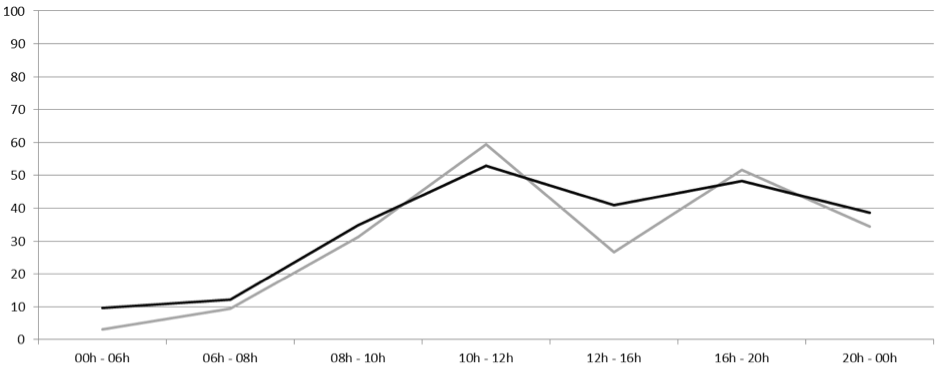
\includegraphics[width=0.9\linewidth]{img/survey_fig2}
     \caption{Motivation to learn during the day. Smartphone users (black line) vs non-smartphone users (grey line)}
     \label{survey_fig:2}
\end{figure}
A study by \cite{Eoff2011} based on one-week click data from Bitly (online link tracking platform) concluded that tablets (iPads) usage during the day is not flat and drastically different when compared to other types of devices, including smartphones and portable computers. Their results suggest that usage lowers after breakfast, remains low during traditional working hours and does not peak until much later in the evening (19 h�00 h). The results of the questionnaire for lifelong learners suggest that there is an association between tablet users and their motivation to learn. The percentage of tablet users motivated to learn was 10\% higher than with individuals that do not use tablets (see Figure \ref{survey_fig:3}). In relation to the peak observed late in the evening by \cite{Eoff2011}, our results show that the learning-motivation-curve in tablet users in the last hours of the day does not descend so much in comparison to non-tablet-users.
\begin{figure}
     \centering
     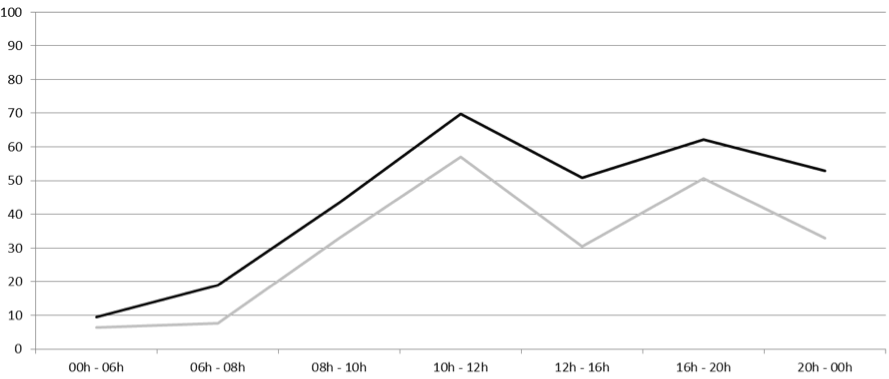
\includegraphics[width=0.9\linewidth]{img/survey_fig3}
     \caption{Motivation to learn during the day. Tablet users (black line) vs non-tablet users (grey line)}
     \label{survey_fig:3}
\end{figure}
\cite{Eoff2011} suggest that tablets are mainly used for entertainment purposes since they are less used than the rest during working times. Tablet usage is higher than the rest of the devices during leisure time. This effect can be also observed during the weekend when tablets usage between 8 h and 15 h is higher than during the week at those same hours. No other device sees a heavy increase of use during the weekend.

When asking lifelong learners on which days of the week do they spend more time with their mobile device(s), our results show (see Figure \ref{survey_fig4}) that the usage for smartphone users is flat with a slight peak on Friday as well as a higher percentage in contrast to non-smartphone users. There is an increase of 30\% in non-smartphone users from a working day (Thursday) to weekend day (Saturday).

There are different ways of consuming learning content on mobile devices: \textit{listening, reading, writing, watching}, and \textit{gaming}. When lifelong learners were asked how long on average they spend on each of these activities, 21\% of the individuals reported to listen more than one hour per day to their mobile devices. This preference for listening can also be inferred from the results in which 64.62\% of the respondents reported to use their media players at least once a week.

When lifelong learners were asked how much time they do spend on different topics per day, the outcome was that \textit{study}, \textit{music} and \textit{social networking} are the activities on which they spend most of their time. In contrast to these results, the study performed by \cite{Arbitron2011} with similar topics indicates that messaging, browsing, social networking and voice are the activities on which individuals spend more time.

Examining the way in which individuals check their mobile phone for a new SMS, missed call, email or any other notification, there are two different behaviours that can be highlighted from the results of the questionnaire. There is a first group of individuals (37.41\%) that only check incoming notifications when the device notifies them with an alert. The second behaviour is performed by the individuals (34.68\%) that check it continuously (at least once per hour). Comparing behaviours between genders, it is remarkable that the option \textit{I only check my mobile when it alerts me} was answered by 44\% of the men and 28\% of the women. Women's behaviour was more evenly distributed among the rest of the options (once a day and once every four hours).
\begin{figure}
     \centering
     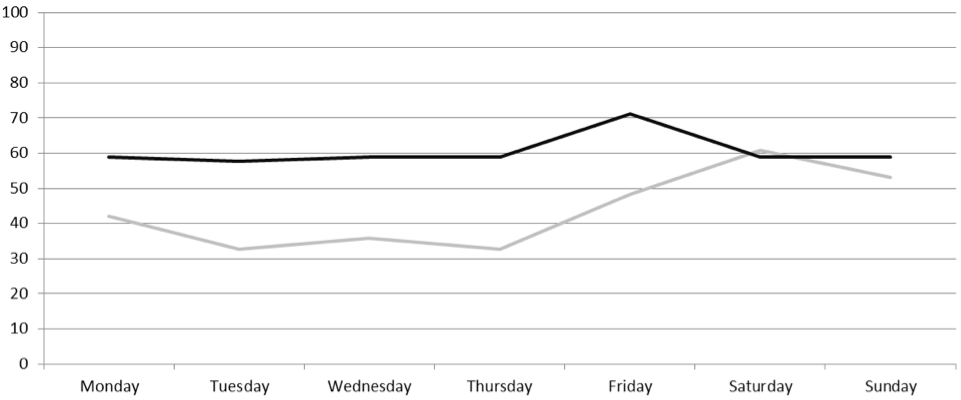
\includegraphics[width=0.9\linewidth]{img/survey_fig4}
     \caption{Mobile device(s) usage during the week. Smartphone users (black line) vs non-smartphone users (grey line)}
     \label{survey_fig4}
\end{figure}
\subsubsection{Linking locations, activities and ways of interaction with mobile devices}
A study performed by \cite{Google2011} on 5013 adults, concluded that there are two main situations where they use smartphone: 1) being at home (93\%); 2) on-the-go (87\%). Moreover, adults were asked for the most common context in which they use Internet on their smartphone. The highest rate was obtained (59\%) for the activity \textit{Waiting} (in the line at the market, doctor, office, bus, etc.). This questionnaire has focused on three learning contexts (at home, on the move, and waiting times) including six items to identify patterns linking locations (living room, kitchen, bathroom, working/sleeping room, on-the-move, and waiting for someone), actions normally performed in those locations (e.g. having breakfast, brushing your teeth, lying on bed, etc.), and ways of interaction with mobile devices (listen, watch videos, write and read), also defined as \textit{learning activities} by \cite{tough1979adult}. These results have raised some interesting differences regarding the way in which participants reported to behave depending on their gender.
\subsubsection{At home}
\textit{Sitting in the sofa} is the most popular place to interact with mobile devices, not only compared to any activity performed in the living room or anywhere at home, but also outdoors and on-the-move. Exactly 62.58\% of respondents reported that they normally \textit{read} contents, 50.34\% \textit{write} contents, 44.89\% \textit{watch} videos and 34.01\% \textit{listen} to audios while being in the sofa. The \textit{living room} was reported to be the most popular place to read contents, and specifying more, \textit{ being sat in the sofa} and \textit{watching TV during advertisement time} (47.61\%). There was also a high rate of respondents that reported to write contents while \textit{watching} TV during advertisement time (32.64\%).

One finding that can be gathered from responses regarding the context \textit{in the bathroom } is that this intimate place has a significant association with mobile device interaction when used for listening. Individuals reported to listen while having a shower (23.12\%), making-up/shaving (18.36\%) and brushing their teeth (18.36\%). Being on the toilet is the most compatible activity with the different ways of interaction, i.e. 33.33\% of the respondents used their mobile device to \textit{read}, 21.08\% to \textit{write} and 11.56\% to \textit{listen}. Similar, the poll performed by \cite{Google2011} stated that 39\% of the adults had used the Internet on their smartphone while \textit{using the bathroom}, and 8\% while taking a \textit{shower/bathing}.

The majority of the respondents (54.42\%) reported that they normally read contents on their mobile devices while \textit{being sat at the desk}, 51.69\% \textit{read}, 37.41\% \textit{listen} and 29.92\% \textit{watch videos}, this means that the \textit{desk} is the best place to interact with mobile devices while \textit{being in the room}. Furthermore, the \textit{bed} is suited to interact with mobile devices \textit{reading} (50.33), \textit{listening} (34.69), \textit{watching} (34.01\%) and \textit{writing} (33.32\%).

The \textit{kitchen} is a location associated with \textit{listening} on mobile devices. The results from this questionnaire suggest the same effects than the ones observed to the context in the bathroom where mobile devices are mainly used for \textit{listening}. The main contexts in which participants embed their listening-learning-activity are while \textit{cooking} (30.6\%) and \textit{heating the breakfast} (25.84\%). It is only remarkable that 16.32\% of the respondents interact with their mobile devices to read contents while \textit{cooking} (probably requesting cook-recipes or short messaging while boiling, frying or anything in the oven). Similar, the survey by \cite{Google2011} indicated that 27\% of the participants had used the Internet on their smartphone while \textit{cooking/and or other household chores}.
\subsubsection{Waiting times}
Rates varied from 15.64\% (being in the airport) to 4.76\% (waiting in a commercial centre). The \textit{bus} stop (43.52\%) and the \textit{train station} (41.49\%) seem to be the most suitable places to interact with mobile devices \textit{reading} contents. When \textit{writing} on mobile devices, the highest rates are evenly distributed (approximately 38\%) for the following contexts: \textit{waiting} at the \textit{bus stop}, at the \textit{train station} and \textit{anywhere in the street}. Results depict that waiting times are not normally used to consume video contents in contrast to the rest of the ways of interaction (listen, read, write). 
\subsubsection{On-the-move}
The results from the study performed by \cite{Kim2005} indicate that the most common context for using mobile Internet is described as follows: \textit{�participants have a hedonic goal, their emotional state is high, their legs are stopped, visual and auditory distractions were low�}, few people are around them, and their interaction is low. This is a different picture from the widely held belief that the mobile Internet would be used often while moving outdoors. However, mobile devices have improved their capabilities to access the Internet, e.g. bigger displays, touch screens and faster connections and mobile interaction with smartphones is different nowadays. Our results suggest that interactions with mobile devices on-the-go are frequently carried out \textit{listening}, being in the train 51.69\%, bus 50.33\%, and walking 48.3\%. \textit{Reading} contents is the second most popular way of interaction when moving, 50.33\% by train, 40.82\% by bus, and 36.73\% accompanying the car driver. The train is the most popular place to interact with mobile devices while listening,\textit{reading} and writing, whereas the plane is the most popular place to \textit{watch videos}. Similar, the poll performed by \cite{Google2011} stated that 43\% of the individuals had used the Internet on their smartphone while commuting to work/school and 20\% driving by vehicle.
\begin{figure}
     \centering
     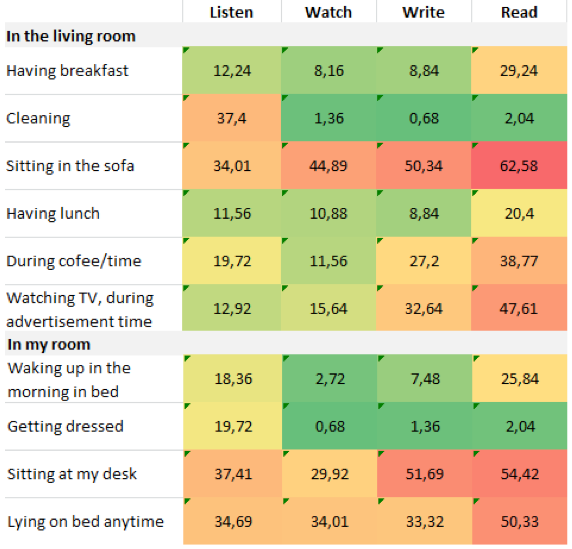
\includegraphics[width=0.8\linewidth]{img/survey_fig5}
     \caption{Learning activities in context with mobile devices. Percentage of individuals. The higher (red) the percentages the more popular the locations/activities are}
     \label{survey_fig:6}
\end{figure}
\subsubsection{Gender}
Regarding the gender effects, our results show some evidence on the fact that certain learning activities were more pronounced in men than women and vice versa (see figure \ref{survey_fig:6}). On the one hand, there are a 44.18\% of men that reported to use their mobile devices \textit{reading} contents while being sat on the toilet; however, only 18.02\% of the women do so. This difference was also notable for \textit{writing} contents (29.05\% men vs. 9.83\% women) and \textit{watching} videos (15.11\% men vs. 3.27\% women). However, gender did not moderate the effects of listening contents. On the other hand, differences were also found regarding \textit{listening} to contents in some particular places. Women reported to be more willing to use their mobile devices while cooking (42.60\% women vs. 22.08\% men), sorting groceries (26.21\% women vs. 5.81\% men) in the kitchen, and cleaning in the living room (49.16\% women vs. 29.05\% men). Moreover, it is remarkable that for the context \textit{waiting} in a commercial centre, 37.24\% of the men reported to read contents in their mobile devices while only 16.38\% of the women reported so.
\begin{figure}
     \centering
     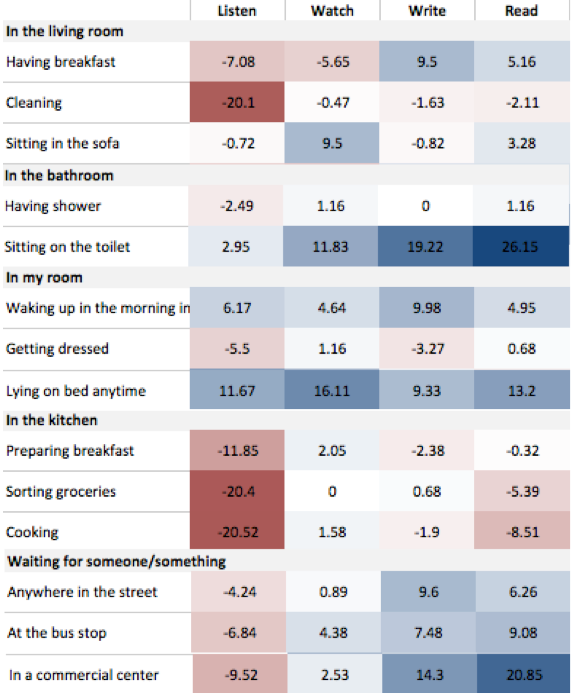
\includegraphics[width=0.8\linewidth]{img/survey_fig6}
     \caption{Learning activities in context with mobile devices. Difference in percentages between men and women. Positive (blue) numbers represent higher male percentage. Negative (red) numbers represent higher female percentage}
     \label{survey_fig:6}
\end{figure}
\subsubsection{More learning activities}
Participants were asked whether they had missed in the questionnaire any other activity where they usually get along some learning episode using their mobile devices. Some of them reported sport activities like running, cycling or at the gym, on-the-go activities like taking a walk or walking the dog, and some other miscellaneous ones like having lunch/dinner alone in a bar, feeding the infant, taking care of the infant, and while doing some do-it-yourself labour at home (carpentry, plumbing...). Similar, the poll performed by \cite{Google2011} concluded that 48\% of the adults had been eating while using the Internet on their smartphone, 17\% walking their dog and 13\% playing sports. Another respondent reminded us that there are no patterns for every situation reporting: \textit{�I just learn something when I find the time�}.

\subsubsection{Difficulties learning with mobile devices}
\cite{Wong2011d} identified ten seams by which learning experiences are disrupted today and for which Mobile-assisted Seamless Learning (MSL) technology has to find new solutions. The identified ten gaps (MSL1-10) in seamless learning support are of high relevance for lifelong learners. Participants were asked about seven of these ten gaps in two items of the survey. The remaining three gaps (MSL5, 9, 10) were too complex concepts to deal in this poll and will be treated in suitable future studies.

In previous sections we have provide evidences to confirm the existence of barriers to learn: across location (MSL4) and across time gaps (MSL3). Some cues are also exposed on how to cover these gaps supported with mobile technology. Participants were requested to report how often do they encounter these difficulties (MSL1-3 and MSL6-8) when learning and assisted with their mobile devices. The results from the questionnaire indicate that participants varying from 12\% to 17\% in the different MSLs usually find these difficulties. Nevertheless, approx. 34\% of the respondents reported not a difficulty in all these difficulties. The most reported difficulty was \textit{finding suitable slots of time during the day} with a 21.08\% of the respondents that reported to have it usually and a 4.76\% that find it always. Slightly higher rates to the three resting difficulties, and with similar rates between them were the \textit{combined use of multiple device types (laptop, mobile phone and/or tablet)} and the \textit{linking real world to what I learned digitally} with approximately 17\% of the respondents that usually found these difficulties.

\section{Conclusions}
The aim of the questionnaire for lifelong learners is to analyse daily learning activities in adults to recognise patterns in lifelong learners and shed light on ways to support them with technology. The analysis of the results arises the ten following findings:

\begin{figure}
     \centering
     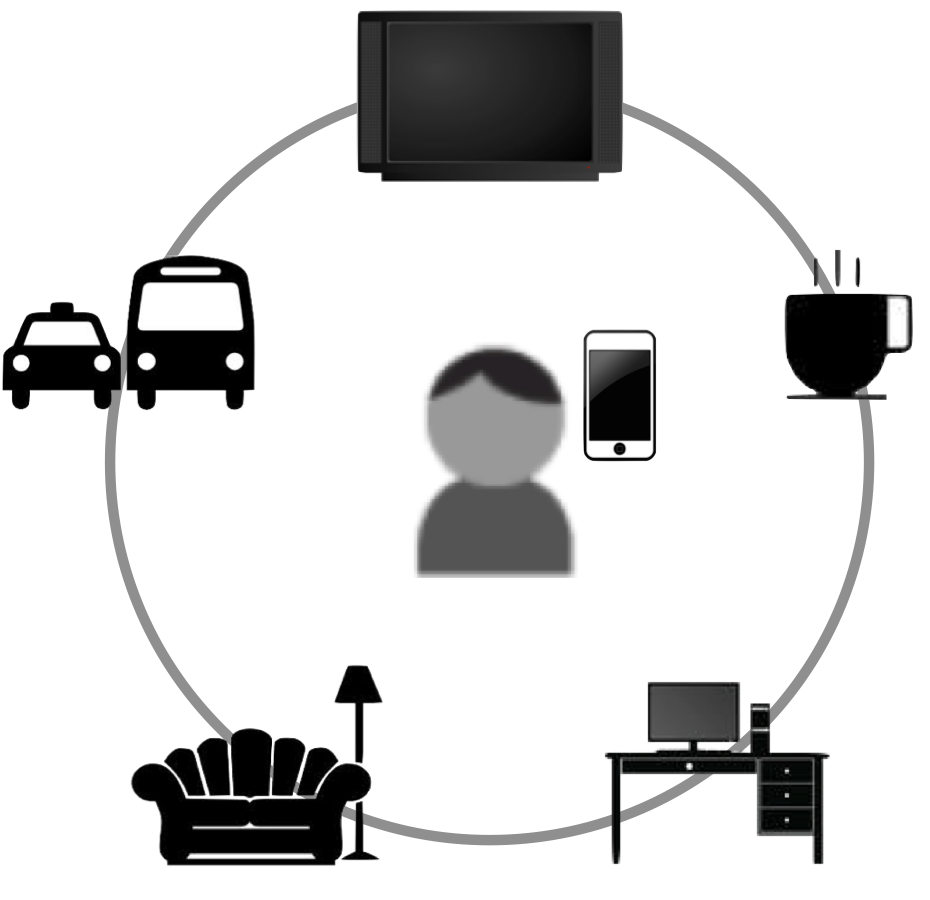
\includegraphics[width=0.5\linewidth]{img/survey_fig9}
     \caption{User's learning environments throughout the day}
     \label{survey_fig:6}
\end{figure}

\begin{enumerate}
\item Portable Computers are the most commonly used device for learning. Recent studies \citep{Wesel2011} have found similar results arguing ergonomic reasons. Students prefer bigger screen in contrast to smaller screens from smartphones or tablets.
\item Individuals that own a smartphone reported to be more constantly motivated to learn during the day than non-smartphone users.
\item Individuals that own a smartphone use it constantly during the whole week. The rest of the individuals reported lower usage during working days and an increase during the weekends.
\item \textit{Listening}  is the most compatible learning activity when performing other tasks at the same time. It is also the one in which adults spend more time and in longer time slots. These results envision that audio contents are well suited for distributing learning materials as they can be consumed from most devices.
\item There are two different behaviours when adults check their mobile phone for a new SMS, missed call, email or any other notification. There is a group that only checks incoming notifications when the device notifies them with an alert. There is another group that check it continuously. These results suggest that these two behaviours must be taken into account when designing mobile applications for learning. 
\item There is an association between the learning activity being performed (\textit{reading, listening, writing or watching}) and the concrete location where it takes place. Some patterns were found in the way to interact with mobile devices while being at home and depending on the room where the individuals were located. Participants were more willing to perform any kind of activity with their mobile device(s) while being in the living room or in the sleeping/working room. Nevertheless, participants reported that the kitchen and the bathroom were places where they use to perform the \textit{listening} learning activity.
\item Learning activities are mainly performed when adults are with their legs stopped. The \textit{reading} and \textit{writing} learning activities mostly take place being sat (sofa, desk, train, bus and toilet) or lying on bed. Sitting in the sofa is the place where adults reported the higher acceptance when carrying out any learning activity. However, the \textit{listening} learning activity takes part more evenly in the different locations and embedded within different activities.
\item Men and women behave different when making use of their mobile devices. These results suggest that men and women seem to behave differently in the way they perform learning activities as well as the way to dispatch incoming notification on their mobile phones. Furthermore, the study performed by \cite{Ofcom2010} stated that men spend nearly an hour more per day using media than women.
\item Lifelong learners reported that their learning experiences are disrupted. \textit{Finding a suitable time slot to learn during the day} is the most frequent difficulty reported by participants. These results are consistent with the ones by \cite{Eurostat2012} suggesting that there is a need to integrate learning activities in daily life.
\item There is a high rate of individuals that are not familiar with the meaning of lifelong learning.
\end{enumerate}

Based on the idea that the opportunity to learn and to grow is all around and should not be a chore for lifelong learners, we will extend this research creating a learner-centred model in which users will be able to interact with smart objects, ambient learning displays \citep{Borner2013} and tagged physical objects that could trigger different activities and lead to learning events. This model will define how channels and artefacts can be linked in order to adapt and serve the information according to adults preferences (location, embedded in learning activity, time of the day, duration of the task, gender, etc.).

		\chapter{OER in the mobile era: Content repositories' features for mobile devices and future trends}


\vfill
Open content will have an impact on education in the short term due to the current trend of offering educational resources for free on the web \citep{TheNewMediaConsortium2010}. Nowadays, a big proportion of the learning materials are accessed from mobile devices. Hence, OER repositories should adapt their capabilities to provide access from mobile devices. This chapter explores common practices in the creation, publication, discovery, acquisition, access, use and re-use of learning objects on mobile devices based on a literature review from 2007 to 2012. From the content providers side, we present the results from a survey performed on 23 educational repository owners prompting them to answer about their current and expected support on mobile devices. From the content user side, we identify features provided by the main OER repositories and relevant apps existing in commercial markets. Finally, we introduce future trends and cues for further research.
\vspace{3em}

This chapter is published as:  Tabuenca, B., Drachsler, H., Ternier, S., \& Specht, M. (2012, December). OER in the Mobile Era: Content Repositories� Features for Mobile Devices and Future Trends. \em Europe elearning papers, Special issue on Mobile learning \em

\clearpage

\section{Introduction}
In 2004 \textit{Learning Objects} (LOs) have been named in the Horizon report as one of the relevant technology trends \citep{Nmc2004}. Six years after, this technology appears again as \textit{Open Content} in \citep{TheNewMediaConsortium2010}, predicting to have an impact in the short term due to the current trend of offering open content for free on the Web. 

Open Educational Resources (OERs) not only comprise LOs, course materials, content modules, and collections, they also include tools for creating, delivering, using and improving educational contents. \cite{chitwood2002} defined LOs with five characteristics: 1) small units of learning, typically ranging from 2 minutes to 15 minutes; 2) self-contained, each learning object can be taken independently; 3) reusable, a single learning object may be used in multiple contexts for multiple purposes; 4) can be aggregated, learning objects can be grouped into larger collections of content, including traditional course structures; 5) are tagged with metadata, every learning object has descriptive information allowing it to be easily found by a search.
 
The advent of mobile technology and the boom in 2007 with the birth of the smartphone have boosted new ways of interaction. Mobile devices are equipped with capabilities (text editor, audio recorder, video recorder, sensors, Internet access, apps, etc.) that facilitate enormously the possibilities to create, publish, discover, acquire, access, use and re-use of educational resources. By mobile device we do not only refer to cell phones, but also to tablets, MP3s, MP4s, game consoles and portable computers. Mobile devices play an important role for lifelong learners enabling different educational scenarios and contexts in which learners can operate \citep{Tabuenca2013}. Hence, mobile devices facilitate ubiquitous access to OERs stored in content repositories.

In the last years, the usage of mobile devices has grown in many application fields of education. Likewise, a big proportion of the learning contents are now 'consumed' from mobile devices. OERs are normally stored in open repositories facilitating search, retrieval and re-use among educational communities. The work from \cite{Su2011} summarizes research on adapted mobile content delivery based on mobile capabilities, learners� preferences, and network conditions. 
So far no work was found synthesizing how OER repositories are adapting to mobile learning. Hereby, we extend the research exploring what features are being provided by OER repositories to facilitate access from mobile devices.

This chapter is organized as follows. Section two explores common practices in the creation, publication, discovery, acquisition, access, use and re-use of learning objects on mobile devices based on a literature review of scientific research from 2007 to 2012. The third section presents the results from a survey performed on 23 educational repository owners prompting them to answer about their current and expected support on mobile devices. Section four analyzes the features that the main OER repositories are providing for mobile support. Finally, section five presents discussion and conclusions.
\section{Literature review on learning objects for mobile devices}
\subsection{Method}
Five major digital libraries were selected to find relevant papers in the usage of mobile devices to access OERs repositories: ACM, IEEE, Science Direct, Springerlink and Wiley. We searched the listed libraries constructing search-strings that follow the pattern: all papers published after 2006 that contain (�Mobile� AND �learning� AND �object� AND �repository� AND �content� AND �education�) in their full-text AND (contain (�mobile�) in their keywords OR contain (�mobile�) in the title). 

This query reported the following number of items: 21 in ACM; 165 in IEEE; 26 in ScienceDirect; 36 in Springerlink; 12 in Wiley. For each of these libraries, results were ordered by relevance and the 20 first elements were extracted. The resulting list of 92 papers was manually reviewed. 
\subsection{Results}
\subsubsection{Creation of contents}
Nowadays, mobile devices are equipped with features that facilitate the creation of learning contents. Indeed, most mobile users are capable of recording audios, recording videos or composing a text note. The quality of the audio and video reproducers, and the increase of the size of the screens to display text, has augmented considerably the degree of excellence for consuming contents with respect to the pre-smartphone era. The exploratory study by \cite{Churchill2008} describes considerations to take into account when designing LOs for small-screen handheld devices. 
\subsubsection{Publication of contents}
Standards are being periodically reformulated to adapt the publication of LOs in content repositories. Tagging resources with meta-data is essential to guarantee their reusability. The need for analyzing the issues that raise the inclusion and use of metadata in the learning objects delivered to mobile devices was already pinpointed by \cite{DeMarcos2006} as a research line pending to develop. For example, the IEEE LOM specification does not directly support the description of educational resources in terms of their relevance to language learning and mobile-delivery related characteristics as claimed by \cite{Sampson2008}. 

Keeping the standards up-to-date is key for teachers and instructional designers to author, search, acquire, (re)-use and share educational resources effectively.
\subsubsection{Content allocation}
This review has resulted in the following ways to filter contents by context and access it from the mobile device: GPS, compass, Wi-Fi, RFID, infrared, barcode, Bluetooth, text recognition and image recognition. 

\cite{Han2007} used mobile indexed image-recognition to augment real images with an extended multimedia description that was stored in an OER repository. Augmented reality has been also implemented using textbooks  \citep{Santana-mancilla2012}. In this work, secondary school students accessed to additional educational contents related to their textbooks. This system recognizes the images printed in the book as part of regular taught topics and shows multimedia contents that complement the topics covered in the book. Similar, \cite{Chao2009} used markers (printed text identifiers) that can be easily read and tracked by a computer to augment text content with multimedia content.

Excursions of art and museum are good examples of content delivery based on the parameters supplied by mobile devices. Mobile guides delivering contextualized audio, video and text are reviewed in recent work from \cite{Emmanouilidis2013}. This work claims that the current trend is to gradually abandon some of the older localization technologies such as Wi-Fi, infrared and manual user position input. \cite{Oppermann1999c} performed the first relevant experiment using infrared for location identification and wireless local netowork for data transmission to and from the server in a museum in which audio contents were delivered from a repository. The near ubiquity of GPS receivers in mobile devices makes this technology extremely popular, nevertheless, they are high battery consumers and they do not work indoors. 

Other localization technologies, such as Radio Frequency IDentification (RFID) and 2D barcodes, have become more popular due to better device support. \cite{Chen2010} featured an augmented reality scenario enriching textbooks with multimedia content stored in a repository. These contents were addressed reading Quick Response (QR) codes printed next to the text to enrich. Similar, \cite{Chen2012,Choi2008,Huang2008} present implementations of contextualized content delivery indexed by RFIDs. 

Near Field Communication (NFC) is an extension of RFID technology. RFID is capable of accepting and transmitting beyond a few meters whereas NFC is restricted to four inches (approximately 10 centimetres). There is a trend  in mobile phones to be equipped with NFC. This type of communication has been evaluated accessing contents stored in OER repositories. A recent experiment implemented a scenario in which a user carrying her mobile phone in a fieldtrip excursion could tap (with her mobile phone) objects augmented with NFC tags. When these tags were decoded by the mobile device, the path to the learning content (i.e. image, video, audio) was decoded and reproduced. Every time a tag was tapped, the action and actor were registered and tracked by the system \citep{Perez-Sanagustin2012}.

\cite{Rahman2011a} implemented a 3D car gaming metaphor to manipulate LOs hosted in repositories, that could be controlled with the gestures identified by the accelerometer of the mobile device (See figure \ref{fig:oerrepos_fig2}). They additionally included a functionality to access, play, and store the learning objects for later browsing through the mobile interface.

\begin{figure}
     \centering
     
\includegraphics[width=0.6\linewidth]{img/oerrepos_fig2}
     \caption{3D car metaphor for navigation between LOs}
     \label{fig:oerrepos_fig2}
\end{figure}

Web browsers keep being the main ways to access LOs  stores in repositories. MERLOT is an example of a portal-based repository adapting the search functionality depending on the type of mobile platform aimed to use the content. \cite{Siadaty} propose the m-LOCO framework for contextualized mobile content delivery, making use of the following repositories: 1) the repository of learning objects includes information about the content format (i.e. audio, video, text) and the educational content types (i.e. exercise, example, overview or tutorial); 2)the delivery media repository contains data about specifications and features of different available delivery media (e.g., mobile devices and PDAs); 3)the context repository is used to perform further analysis or reasoning (e.g., every time a learner selects a learning object from the learning object repository, the related contextual data would be gathered and stored in the repository).

\subsubsection{Standards for content packaging, delivery and sequencing}
IMS Learning Design and the SCORM are the most important interoperability models for reusability in eLearning. This review has identified the following solutions making use of these standards in mobile devices:

\em Pocket-SCORM \em  is a SCORM reader on mobile devices with access to an Learning Management System (LMS) server and a SCORM repository. This tool was first released in June 2004 for Windows Mobile \citep{Chang2005}. To the best our knowledge, the \em Pocket-SCORM\em was not further developed. 

\em SMILE PDA \em  is an open source software implementation for executing IMS Learning Design activities via mobile devices. In contrast to existing IMS Learning Design Players such as Coppercore\footnote{CopperCore, The IMS Learning Design Engine. http://coppercore.sourceforge.net/} and Reload Player\footnote{Reload Project, Reload IMS LD Player. http://www.reload.ac.uk/}, the \em SMILE PDA\em does not need to be connected to the Internet during the entire execution time and has been specially designed for delivery through mobile user interfaces as the educational content can be automatically adjusted to the size of the display of the device used \citep{Sampson2008}.

The \em eXact-mobile \em \footnote{eXact mobile http://www.exact-learning.com/en/products/learn-exact-suite/exact-mobile-solution-for-mobile-learning}  is a commercial solution for standard management, delivery and tracking of multimedia for training. This tool features tracking, synching and content authoring according to recognized standards (i.e. SCORM). This tool supports content delivery for Android, iPhone and Blackberry.

The \em PLCAM \em delivers SCORM mobile LOs based on learners� preferences, hardware profile and �satisfaction degree� of these contents in previous usages \citep{Su2011}.
\subsubsection{Architectures framing mobile content delivery}
In the last years, different service-based architectures have been proposed with the aim to provide educational institutions the flexibility to add and re-use services inside the already existing platforms. This way, many basic services and resources do not need to be developed again, reducing considerably the complexity in the design of new educational environments. \cite{MartinProc2009} in their review of existent solutions propose an architecture (figure \ref{fig:oerrepos_fig4}) in which LMS services are transferred to mobile devices from Web-Services that outsource the resources via HTTP.
\begin{figure}
     \centering
     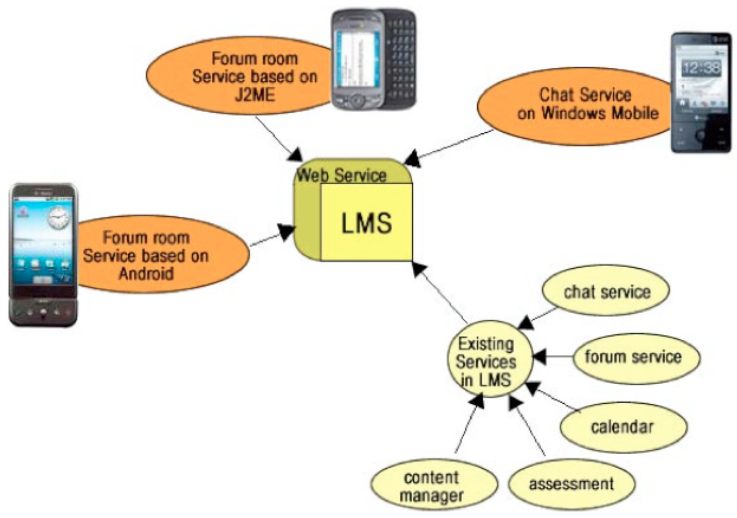
\includegraphics[width=0.6\linewidth]{img/oerrepos_fig4}
     \caption{Integration of LMS services for mobile devices \citep{MartinProc2009}}
     \label{fig:oerrepos_fig4}
\end{figure}
\subsubsection{Content repositories and ubiquitous computing}
Tagging physical objects (books, pictures, sculptures, etc.) with QR codes or RFID tags enriching them with multimedia content has resulted in different implementation in the last years. In most of the cases, the resource repository provides content-related materials that are not originally included in the original physical object. Physical objects can be augmented with texts \citep{Chen2010,Chao2009}, images \citep{Han2007,Santana-mancilla2012} or multimedia \citep{Perez-Sanagustin2012a}. 

This review highlights different examples of ubiquitous computing scenarios broadcasting contextualized learning contents to mobile devices. \cite{Barbosa2007} show how LOs can be delivered to students depending on their physical location and their progress completing a task. More recently, \cite{Rahman2012} designed a prototype that makes use of accelerometer and infrared sensors to select and launch LOs to different displays by pointing at them with the mobile device. 

\section{A survey to OER repositories on mobile access}
This section presents the results of a survey performed on 23 content repositories, partners of the Open Discovery Space  European project, hosting more than 1,583,000 resources (this is an approximation since some of the contents might be overlapped in more than one repository). The aim of this survey is to gain insight into the way content repositories provide access to mobile devices. Table \ref{tbl:oerrepos_tbl1} lists the repositories participating in the survey.

\begin{table}[h]
  \small
  \caption{Content repositories participating in the survey}
  \label{tbl:oerrepos_tbl1}
\begin{tabular}{lllll}
\thickhline
\textbf{Repository} & \textbf{Scope} & \textbf{\begin{tabular}[c]{@{}c@{}}Num of \\ resources\end{tabular}} & \textbf{} \\ \thickhline
ARIADNE federation           		& International teachers \& students          	& \multicolumn{1}{r}{1,000,000}           &           \\ 
Open Science Resources            	& European science teachers           			& \multicolumn{1}{r}{1,200}           &           \\ 
eduTubeplus library            		& European teachers \& students           		& \multicolumn{1}{r}{5,000}           &           \\ 
COSMOS            					& International science teachers           		& \multicolumn{1}{r}{100,000}           &           \\ 
I2G Intergeo           				& European math teachers \& students           	& \multicolumn{1}{r}{3,500}           &           \\ 
Key2Nature�s Dryades             	& European biology teachers \& students			& \multicolumn{1}{r}{86,000}           &           \\ 
OpenScout federation           		& International teachers \& students           	& \multicolumn{1}{r}{53,000}           &           \\ 
SIVECO�s ASPECT            			& Romanian teachers            					& \multicolumn{1}{r}{1,600}            &           \\ 
FUNecole           					& European teachers \& students            		& \multicolumn{1}{r}{1,500}            &           \\ 
LaProf            					& European language teachers \& students       	& \multicolumn{1}{r}{800}           &           \\ 
Miksike�s LeFo            			& Estonian, Lithuanian \& Latvian teachers     	& \multicolumn{1}{r}{50,000}           &           \\ 
Bulgarian repository           		& Bulgarian teachers \& students           		& \multicolumn{1}{r}{3,500}           &           \\ 
Virtual Bulgaria           			& Bulgarian teachers \& students  				& \multicolumn{1}{r}{7,000}           &           \\ 
Znam.bg            					& Bulgarian teachers \& students           		& \multicolumn{1}{r}{100,000}           &           \\ 
BMU            						& Serbian teachers \& students           		& \multicolumn{1}{r}{180}           &           \\ 
Croatian repository           		& Croatian teachers \& students           		& \multicolumn{1}{r}{2,700}           &           \\ 
Greek repository           			& Greek teachers \& students           			& \multicolumn{1}{r}{1,000}          &           \\ 
Bildung.at          			  	& Austrian teachers           					& \multicolumn{1}{r}{500}           &           \\ 
LMS.at 				           		& Austrian teachers           					& \multicolumn{1}{r}{100,000}           &           \\ 
Ambjorn�s Naeve math           		& Math teachers           						& \multicolumn{1}{r}{300}            &           \\ 
OERCommons.org           			& International teachers           				& \multicolumn{1}{r}{70,000}           &           \\ \hline
\end{tabular}
\end{table}

\subsection{Method}
This survey gathers information about repository�s accessibility via mobile devices, potential support with apps and functionalities from the repository�s point of view. Repository owners received an email in which they were prompted to answer six questions related to mobile usage. Guidelines and instructions to fill in the requested information were attached. The collected spreadsheet-files were analyzed obtaining the following results:
\subsection{Results}
Figure \ref{fig:oerrepos_fig7} illustrates the answers reported to the question: Q1.\em Did you prepare your repository to be accessed by different mobile devices?\em . The majority of the repositories (87\%) answered that their repository can be accessed by portable laptops. Tablets are in the second place with 74\% of the repositories. More than 65\% of the repositories are accessible via smartphones. Summarising, more than half of the repositories can be explored by all type mobile devices due to the fact that they were accounting access from a web browser.

\begin{figure}
     \centering
     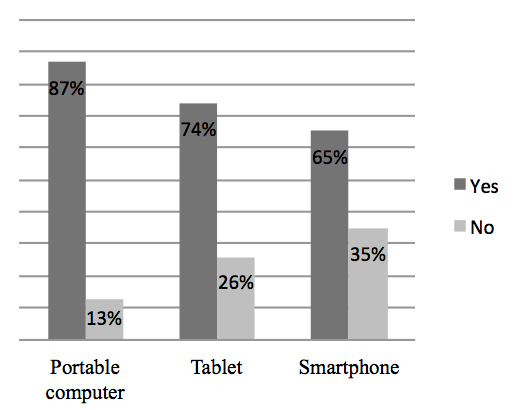
\includegraphics[width=0.5\linewidth]{img/oerrepos_fig7}
     \caption{Question 1: \em Did you prepare your repository to be accessed with different mobile devices?\em. Percentage for n=23 repositories.}
     \label{fig:oerrepos_fig7}
\end{figure}

Contrary to our expectations, the results presented in table \ref{tbl:oerrepos_tbl2} show that the majority of the OER repositories did not consider providing an app to facilitate access from mobile devices. The majority of the owners of the OER repositories reported not knowing a suitable app to facilitate open access from mobile devices. Nevertheless, a big proportion (65\%) of the respondents reported that an app would increase the access rates to their repositories. There is even more consensus in the answers reported to Q5 in which 75\% of the OER repositories indicated that an Application Programming Interface (API) would help them to provide access from different devices.

\begin{table}[h]
  \small
  \caption{Survey to OER repositories}
  \label{tbl:oerrepos_tbl2}
\begin{tabular}{rlrrr}
\thickhline
Q\# & Question                                                                                                                                                                  & Yes  & No   & NA   \\ \thickhline
Q2  & \begin{tabular}[c]{@{}l@{}}Did you consider providing an app to\\ access the content in you repositories?\end{tabular}                                                    & 39\% & 52\% & 9\%  \\
Q3  & \begin{tabular}[c]{@{}l@{}}Do you know any suitable app for accessing\\ content repositories and open content?\end{tabular}                                               & 17\% & 52\% & 30\% \\
Q4  & \begin{tabular}[c]{@{}l@{}}Do you think an app could increase the access\\ rates to your repository?\end{tabular}                                                         & 65\% & 22\% & 13\% \\
Q5  & \begin{tabular}[c]{@{}l@{}}Would you consider providing an application\\ interface (API) to provide access to your\\ repositories from other sites and apps?\end{tabular} & 74\% & 9\%  & 17\% \\ \hline
\end{tabular}
\end{table}

Figure \ref{fig:oerrepos_fig12} illustrates the answers reported to the question: Q6.\em What kind of functionality would be beneficial to feature towards supporting access from mobile devices? \em Average 60\% of the repositories found ranking of the content, social collaboration, and cloud storage as the most beneficial functionalities to provide mobile access. Furthermore, more than 30\% of the repositories agree that the following functionalities are beneficial to support mobile access: location-based services, augmented reality, reading voice services, help documentation, version control, schema representing tools to visually link docs and authors, voice-enabled search.

\begin{figure}
     \centering
     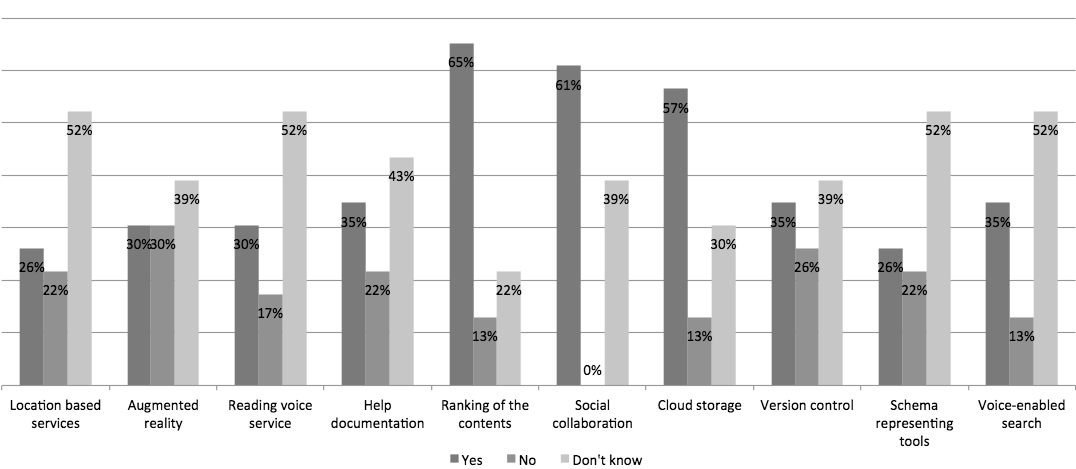
\includegraphics[width=1\linewidth]{img/oerrepos_fig12}
     \caption{Question 6: \em What kind of functionality would be beneficial to feature towards supporting access from mobile devices? \em. Percentage for n=23 repositories.}
     \label{fig:oerrepos_fig12}
\end{figure}

\section{OER repositories' features for mobile devices}
This section reviews specific features provided by OER repositories supporting mobile access. Some of the features described here were discovered in the scientific literature review presented in previous sections. Here, we have selected some of the previously cited OER repositories, to describe which initiatives they carried out for mobile support. Additionally, we review relevant referratories  and projects that were excluded in the previous section. By referratory we mean repositories that only handle metadata from LOs, while the LOs are stored somewhere in a different repository. The method to analyze them was browsing their sites and exploring the main app markets in Internet (i.e. Google Play, Apple Store).

\begin{figure}
     \centering
     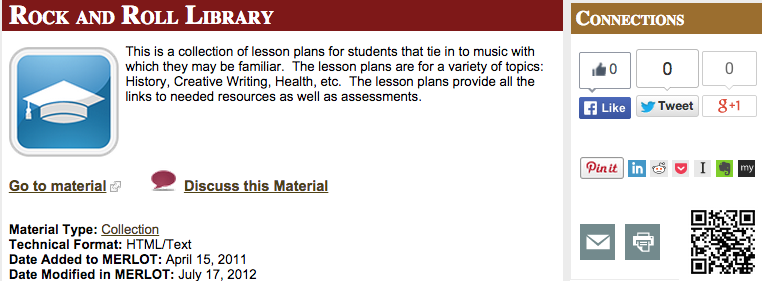
\includegraphics[width=0.9\linewidth]{img/oerrepos_fig15}
     \caption{MERLOT repository. LOs are listed with a QR codes for augmenting paper material.}
     \label{fig:oerrepos_fig15}
\end{figure}

The \em OpenScout \em  Project was launched in 2012 as a portal that provides free online management of OERs, i.e. search, visualize, use, share and publish. The OpenScout features an interface to start a keyword-based search, filter search results, include competence search criteria, or add social metadata like tags, comments or ratings. Regarding the features supporting mobile devices, The OpenScout app for iOS provides a keyword search in which search results are sorted by relevance. The app facilitates access to the details of the resources and bookmark them. Bookmarks are saved locally in the users� device facilitating the organization and collection of items that the user might find relevant.

\em Mobile2Learn \em  is a European Project that aims at improving language-learning instruction by expanding the resources for teaching and learning in vocational education training.  This portal intends to promote access to mobile-supported training services for the provision of on-demand lifelong language learning beyond time and place restrictions. Mobile2Learn provides a stand-alone application (MW-TELL) that can be installed in a PDA or smartphone device and facilitates the delivery of mobile training courses. The main functionalities of MW-TELL Courses PDA include: delivery of mobile training courses packages for English language learning; support of multiples roles, such as individual learners and tutors; rendering of HTML�based content and flash files conformant with the IMS Learning Design (v1.0 Level A specification) and IMS Content Packaging (v1.1.4 specification).  \cite{Sampson2012} present an implementation of the Mobile2Learn framework for English language-learning concluding the following indications: existing Mobile-Assisted Lifelong Language Learning (MALL) resources can be re-used within different MALL courses, while retaining their open access by different platforms and systems; existing MALL course templates can be re-used within different MALL courses addressing teaching of a specific language. The features from MW-TELL are further described in \citep{Romero}.
 	 	 
\em MERLOT \em  is a free and open online community of resources designed primarily for faculty, staff and students of higher education around the world to share their learning materials and pedagogy. MERLOT provides different capabilities for mobile support. The free MERLOT OER search app for iOS and Android-based mobile devices search the MERLOT database for open educational materials. MERLOT OER search app enables mobile users to retrieve detailed, discipline-based information on thousands of open courses, open texts, and open journal articles directly from MERLOT�s internationally renowned digital library.  Retrieved information includes all the comments, ratings, related learning exercises, and peer review information, with links directly to the learning materials in the hit list. It is possible to share findings with colleagues via mobile device. All the materials listed in MERLOT include a QR code with an URL redirecting to the learning materials so they can be easily shared or bound to paper materials (See figure \ref{fig:oerrepos_fig15}). Additionally, MERLOT provides an advanced search for materials designed for mobile devices including the criteria �Type of delivery platform� to the information (metadata on smartphones, tablets, LMS�s). 

\begin{figure}
     \centering
     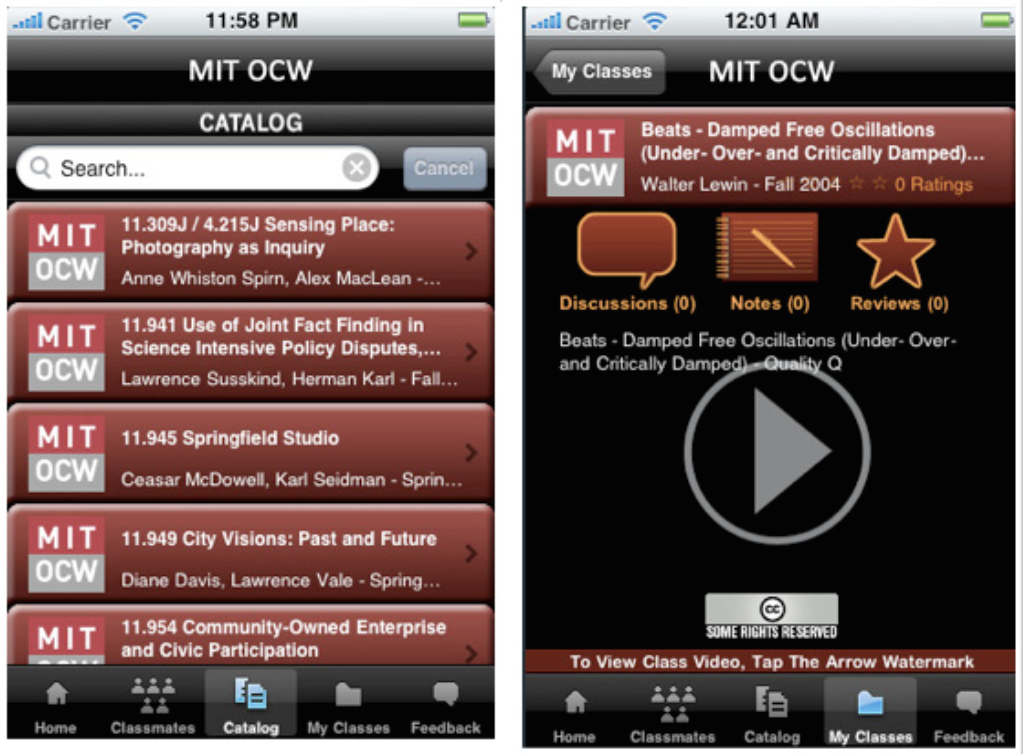
\includegraphics[width=0.6\linewidth]{img/oerrepos_fig16}
     \caption{iOS app for MIT OpenCourseWare}
     \label{fig:oerrepos_fig16}
\end{figure}

\em The OpenCourseWare (OCW) \em movement initially started in T�bingen (Germany), was finally launched at Massachusetts Institute of Technology (OCW-MIT), an open, free, web-based publication of all courses and contents taught at MIT. This initiative has been widely extended to multiple universities around the world. MIT-OCW released their iPhone app in February 2011 (figure \ref{fig:oerrepos_fig16}) allowing to access OCW videos stored in iTunes. Its social learning experience makes this app different from others. This app includes a virtual space called �classmates� where students can discuss with colleagues. 

\em Khan Academy�s \em website supplies a free online collection of more than 3,500 micro lectures via video tutorials stored on YouTube covering a broad range of educational topics. Khan Academy has a higher rate of videos viewed in comparison to MIT's OCW. The Khan Academy launched an official app both for Android and iPhone (figure \ref{fig:oerrepos_fig17}) and iPad app (March 2012). Its main functionality is providing access to videos. There are also unofficial viewer apps that let import the Facebook profile (figure \ref{fig:oerrepos_fig17} right).

\begin{figure}
     \centering
     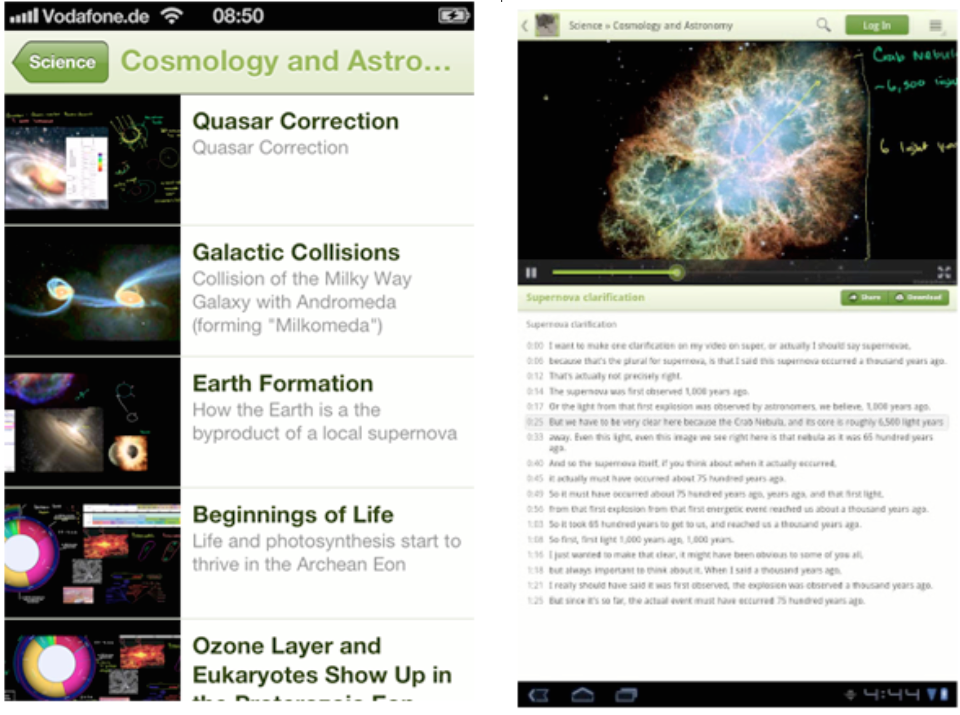
\includegraphics[width=0.6\linewidth]{img/oerrepos_fig17}
     \caption{Mobile apps for visualising videos from Khan Academy. iOS official app (left). Android unofficial app (right).}
     \label{fig:oerrepos_fig17}
\end{figure}

\section{Discussion and conclusions}
Mobile devices facilitate new ways to access content from OER repositories. This chapter has shed light on different prototypes and tools using GPS, compass, Wi-Fi, RFID, NFC, infrared, QR code, Bluetooth, text recognition, image recognition or the accelerometer to index contents stored in OER repositories. These prototypes have been evaluated in different learning contexts \citep{Chen2010,Chao2009,Han2007,Santana-mancilla2012,Perez-Sanagustin2012a,Barbosa2007,Rahman2012}. This study shows cues on how to augment physical objects (books, museums, etc.) with digital learning contents delivered to mobile devices and extracted from content repositories.

Easy to create and consume mobile contents are those whose unit of construction (granularity) is less complex, i.e. text, audio or video. Nowadays, smartphones and tablets are equipped from scratch with tools that facilitate easy creation and consumption of this type of materials, as no special app or feature needs to be installed. Most of the studies reviewed in this chapter pull materials with low granularity. The work from \cite{Yang2007} adapting already existing desktop-based learning materials to the mobile setting advise the use of technologies like HTML5 to make easier integration of audio, video, and texts in mobile platforms (see Khan Academy official app). Adapting more complex contents like LOs to mobile-LOs is hard to maintain in long terms since mobile technology is continuously evolving the features from new mobile devices. Previous LOs were designed and created for desktop platforms and some of their features are missed when moved to a mobile context (screen size, content sequencing, etc.). \cite{Bradley2009} describe this incompatibility as follows: � \em LOs were developed to tackle a series of pedagogical challenges, such as facilitating learner engagement, and aiding students in dealing with problems of abstraction and complexity. These learning objects use a number of constructivist principles provided by rich interactive visualizations or learner controlled pacing \em �. The review of the apps existing in commercial market concluded with no �killer app� adapting desktop-based LOs to for mobile devices. We have highlighted apps sequencing learning contents (e.g. eXact and MW-TELL mobile app), as well as best practices to scaffold architectures to facilitate across platform accessibility (iOS, Android, Windows) compatibility like web-services, APIs, or HTML5.

From the repository� point of view, the results of the survey indicate that the majority of the content repositories are accessible by different mobile devices (via web browser). These results provide an overall view of the extent to which repositories are in a significant need to adapt their architectures for mobile devices rather than adapting the content. Hence, repositories should provide content that can be delivered via HTTP (e.g. via web-services) to any device, as well as following formatting (e.g. HTML5) and sequencing (e.g. SCORM) standards to foster universal access to open communities.

		% To-Dos:

\chapter{Tap it again, Sam: harmonizing personal environments towards lifelong learning} % Write in your own chapter title

%\begin{quote}
%\textbf{Abstract:} With a focus on the situated support of informal and non-formal
%learning scenarios in ubiquitous learning environments, the presented paper outlines the authors� vision of ambient learning displays � enabling
%learners to view, access, and interact with contextualised digital content
%presented in an ambient way. The vision is based on a detailed exploration of
%the characteristics of ubiquitous learning and a deduction of informational,
%interactional, and instructional aspects to focus on. Towards the vision essential
%research questions and objectives as well as a conceptual framework that
%acquires, channels, and delivers the information framed in the learning process
%are presented. To deliver scientific insights into the authentic learning support
%in informal and non-formal learning situations and to provide suggestions for
%the future design of ambient systems for learning the presented paper concludes with a
%research agenda proposing a research project including a discussion of related
%issues and challenges.
%\end{quote}
\vfill
The increasing number of mobile vendors releasing NFC-enabled devices to the market and their prominent adoption has moved this technology from a niche product to a product with a large market-share. NFC facilitates natural interactions between digital world and physical learning environments. The scaffolding of learning ecologies is a key aspect for lifelong learners in their challenge to integrate learning activities into busy daily life. The contribution of this manuscript is twofold: first, a review of scientific literature in which NFC has been used with a direct or indirect purpose to learn is presented, and potential uses for learners are classified according to their type of interaction; based on these findings the NFC MediaPlayer is presented as an instantiation of an ecology of resources (EoR) in a lifelong learning context. Finally, shortcomings and best practices are highlighted in the conclusions, and future work is discussed.
\vspace{3em}

This chapter is published as: Tabuenca, B., Kalz, M., \& Specht, M. (in press). Tap it again, Sam: harmonizing personal environments towards lifelong learning. International Journal of Advanced Corporate Learning (iJAC)
\clearpage

\section{Introduction}
In a survey by the European Commission time, location and conflicts with other activities have been identified as the core barriers to lifelong learning \cite{EuropeanCommission2007}. Lifelong learners constantly re-design their environments to optimise opportunities interacting with social and other resources towards their learning goals. However, there is little technological support for lifelong learners that typically try to learn in different contexts, are busy with multiple parallel learning tracks, and must align or relate their learning activities to everyday leisure and working activities \cite{Kalz2014}.

On the other hand, visions of ambient intelligence emphasize on the importance in the natural interaction between user and services embedded in the environment or available through mobile devices. \em Natural User Interfaces \em and the \em Internet of Things \em have been predicted to have an impact on education in the short term \cite{Johnson2012}. Tagged objects are widely accepted and the number of connected devices could reach 50 billion by 2020 \cite{Ericsson2011}. Different tagging methods (e.g. visual codes, text recognition, image recognition) allow enriching physical objects with educational resources \cite{Specht2013}. In particular, the prominent adoption of Near Field Communication (NFC) readers in mobile devices has moved this technology from an innovator to an early adopter phase. The NFC Forum\footnote{NFC Forum. Since 2004, this organization develops specifications to ensure interoperability among devices and services. http://nfc-forum.org/} has recently (as of October 2014) estimated that more than 70\% of all smartphones will be equipped with NFC in 2018 \citep{Bialke2014}.

Lowering the barriers for access to relevant information and support services in frequently used living spaces represents an essential challenge for lifelong learning support. Hence, lifelong learners normally build personal ecologies with the resources available in the environment to support their learning needs. In this scenario, the smartphone plays the role of a hub connecting smart resources coexisting in personal learning environments.

This manuscript aims at gathering previous work in which NFC technology has a potential for learning. This collection aims at inspiring scaffolds to create ecologies of resources in personal learning environments. The document is distributed as follows. Section 2 reviews scientific literature in the field of NFC with a special focus on empirical research. Previous work is classified based on the type of NFC interaction implemented. Taking into account lessons learned in the literature review, section 3 presents a NFC ecology comprising different resources in a frequent learning scenario.
\section{Literature review in NFC technology for learning}
NFC is a radio technology that supports transactions at distances of a few centimetres. NFC standards cover communications protocols and data exchange formats based on existing Radio-Frequency IDentification (RFID) standards. In the current review, we have covered both terms since NFC is an extension to RFID technology. RFID is capable of accepting and transmitting beyond a few meters while NFC is restricted to within four inches.

The underlying search was conducted utilizing the online research repositories of the ScienceDirect, Springer, as well as the IEEE Computer Society. The focus on these repositories is reasonable as they cover a sufficiently large number of relevant publications. Within the Springer digital library an advanced search was performed in December 2014 querying all articles of type journal, proceeding, or transaction that had been published since 2007 (when the first NFC enabled mobile phone was released\footnote{Nokia 6131 NFC phone taps into mobile payment, ticketing and local sharing. Press. http://bit.ly/1stNFC}) and matching the keywords � \em (NFC learning mobile) OR (RFID learning mobile) \em � as part of the body. The first 100 occurrences ordered by relevance were selected. In a first round, these items were filtered by title and abstract. In a last round, the resulting manuscripts were filtered according to their educational potential. The rest of the repositories were analysed analogously. This review does not aim to be accurate and strict, but rather exploratory to identify suitable learning scenarios and the type of interaction among the resources that better fits the scaffolding of personal learning ecologies with NFC technology.

There are three devices that can be involved in NFC communication: 1) an NFC-enabled mobile device; 2) an NFC external-reader; 3) an NFC tag. NFC mobile phones and NFC external readers can read NFC tags but also other NFC mobile phones working in passive mode. NFC mobile can write NFC tags (Table \ref{tbl:table1}). As a result of this review, previous work is classified (Table \ref{tbl:table2}) according to the type of NFC interaction implemented and best practices are highlighted.

\begin{table}[h]
  \centering
  \small
  \caption{Type of interaction with NFC devices}
  \label{tbl:table1}
\begin{tabular}{lllll}
\thickhline
\textbf{Active device} & \textbf{Action} & \textbf{Passive device} & \textbf{} \\ \thickhline
NFC mobile phone           		& Reads          		& NFC mobile phone           &           \\ 
NFC mobile phone            	& Reads and or writes   & NFC tag           &           \\ 
NFC external reader            	& Reads           		& NFC mobile phone           &           \\ 
NFC external reader    			& Reads           		& NFC tag           &           \\ \hline
\end{tabular}
\end{table}




As a result of this review, scenarios and resources are classified in Table \ref{tbl:table1} according to the type of NFC interaction implemented.

\subsection{Formal Education}
Recent work \citep{Ebner2013}, envisions some of the potentials NFC technology brings for teaching and learning materials in formal education, with a special focus on connecting digital media and printed learning resources: 1) Distributing learning materials in face-to-face classrooms. Transferring the files from teachers (NFC tag) to students (NFC mobile) avoiding printing on paper and delivering them manually; 2) Enriching printed materials. NFC tags stuck on printed materials facilitate the association of multimedia content; 3) Sharing materials among students. Peer-to-peer communication between mobile devices; 4) Signing delivered practical work and handing it in. For instance, when a student delivers a practical work, the teacher scans the student�s tag with the NFC reader to confirm his/her identity and automatically submits back an email to the student as acknowledgment of reception; 5) Integration with social networks i.e. tap a tag to log in a social network the timestamp in which the arrives to school; 6) Control materials. Teachers can tag the tools in a lab in order to control which resources are assigned to each student; 7) Examinations. NFC tags can be stuck to identity cards from students so teachers can verify their identity in exams.

An introductory course in systems engineering \citep{Gomez2013} used hardware components enriched with tags, to provide multimedia resources such as hypertext, audios, videos and animations describing their functionality within the computer. Their experiment concluded with increased learning outcomes for the group of students using this self- paced mobile approach in contrast to the group using the traditional face-to-face lecture.

Similar, \cite{Riekki2013} implemented a pilot study to support children in their efforts in learning to read. Different words written on a poster and a NFC tag attached to them, provided the audio version of the word when the tags were tapped. The results of the pilot study suggested that NFC is a suitable technology for learning to read as a consequence of a positive effect on children�s emergent letter knowledge.
\subsection{Guided tours and fieldtrips}
Excursions of art and museums are typical scenarios where content is delivered based on the parameters supplied by the mobile device. Mobile-guides delivering contextualized audio, video and text, are reviewed in recent work \citep{Emmanouilidis2013}. This work claims that the current trend is to gradually abandon some of the older localization technologies such as Wi-Fi, infrared and manual user position input. Most of the times, a guide is not necessary because visits to museums are mostly in small groups, and visitors do not want to be overloaded with information. RFID interaction offers a non-intrusive and intuitive interaction in which the user can customize his own learning by approaching the smartphone to a tag attached to a physical object based on his interests on a concrete author, topic, age, etc.

Visitors with limited motivation prefer a broader presentation in contrast to visitors who express an additional interest. \cite{Kuflik2011} implemented different tours and multimedia presentations adapting the content delivered based on the motivation of the visitor. This work concludes the use of RFID as the simplest available technology for accurate customization and positioning inside a building. Previously, \cite{Miyashita2008} had combined RFID tags, and a mobile-PC to use already existing audio guides during a six-month exhibition on Islamic art. Similar, in the work from \cite{Garrido2011} students used NFC enabled phones in the context of a mobile game to know the university campus. Students tapped tags whenever they wanted to communicate to the central game manager their progress within the game and get follow-up assignments. The work from \cite{Sanchez2011a} presents the results of a prototype evaluation that aimed at persuade students to do physical exercise exploring points of interest in the surroundings and tapping them.

Posters can be augmented with different NFC tags to provide a specific feedback based on the tag that is tapped. In the context of a gym in a university campus, Andersen et al. \cite{Andersen2013} created a full size smart-poster with the different muscle groups. When exercising, the user can select a muscle group by tapping that part of the poster so that the information describing training tips for this muscle group is displayed as well as training videos demonstrating some possible exercises.

Interactive panels in public spaces can be used to support social activities. A novel solution \citep{Tesoriero2014} based on the concept of collaborative interactive panels facilitates users sharing their opinions and votes about environmental concerns tapping the panels with NFC-enabled mobile devices.

The work from \cite{Tabuenca2014d} on mobile authoring stresses the importance of knowledge and skill acquisition in the same context in which they need to be performed. Hence, the paper pinpoints to NFC tags as a suitable storage for mobile-authored Open Educational Resources (OER) in public spaces as they can be easily dropped, shared or remixed by different users and inspired by the authenticity of learning in context.
\subsection{User identification}
Badges are usually integrated in identification cards to track and locate persons in buildings, floors or rooms with different access policy. Sometimes students cannot access certain resources of a lab outside of a defined schedule or teachers can only access the facilities supplied by their department. Traditional keys are increasingly being supplanted by identification cards that give access to certain places depending on the profile of the user. 

\cite{Sandberg2005} provide a real time unauthorized access alert to clinical staff by integrating instant messaging technology and RFID. If teachers would use this technology, students would be able to locate in which classroom a teacher is giving a lecture. Occasional changes of classroom would be detected by the presence of the teacher in a different classroom, so that a SMS notification would be sent to the students, or displayed on digital boards. Analogously, this technology can be used by parents/teachers to have a real-time account on when do their children/students go to class.

NFC tags are increasingly embedded into wearables like key-rings, bands, clocks, collars, or bracelets. Theses tags can be read through material such as wallets and clothing. The GerAmi system \citep{Corchado2008} provides insights on how this technology can be successfully applied in wearables. The objectives of this system are to monitor patients and manage the work of the doctors and nurses. The system is configured with ID-readers above each door in rooms and elevators in the facility. Nurses and Alzheimer patients wear a bracelet containing an RFID chip. Additionally, nurses are equipped with PDAs in order to follow the information, set controllable alarms and locks. Additionally, these hospitals provide wireless access points.

In \cite{Andersen2013} key locations at the campus like caf�s, lecture halls and meeting points, are tagged with NFC tags to check-in when entering these locations. This action is registered in a social network (Foursquare. a social networking layer that enabled a user to share their location with friends, via the "check in" - a user would manually tell the application when they were at a particular location. \footnote{https://foursquare.com}) so friends are aware when a person arrives and to a location i.e. for coffee breaks.

A smart classroom system integrates NFC technology to automate attendance management, locate students, and provide real-time feedback via personal response systems \citep{Shen2014}.
\subsection{Activity recognition \& life logging}
The work from \cite{Yang2011a} uses RFID technology to identify which activity the user is doing. The operations in their activity theory consider three arguments: \em object, location, and time \em. \em Object \em refers to tangible things that humans can interact with (e.g. dishwasher, fridge, microwave). \em Location \em represents the environmental information where an operation occurs. \em Time \em is the duration over which an operation was conducted. This information can be later analysed to identify behavioural patterns.

The work from \cite{Castro2014} explores behavioural data gathering for assessing functional status and health of older adults using NFC enabled mobile phones.  Participants were provided with a deck of twenty NFC-cards depicting some of their most common activities such as going to the supermarket, cooking, watching TV, or going to the doctor. Finally, they were also given a booklet to jot down the time in which the activities were carried out. The mobile devices were carried around older adults� waists.

More recently, \cite{Curiel2013} propose a platform that activates the most used services on mobile devices, such as making a call, by interacting with NFC tags. Thus, depending on the combination of tags users read, the system will recognize the service to activate (read email, send email, telephone call, see photos, show weather forecast, see news and share information) and the parameters needed for its execution (news source, contact email, phone number).

The NFC LearnTracker \citep{TabuencaLT2014b} is a tool for self-regulated learning that facilitates the introspection of learning patterns via analytics. This tool is built assuming that commonly used learning materials are tagged with NFC tags. The student taps the tag every time he starts and stops learning, these timestamps are recorded, and the activities can be later analysed with chart visualizations upon their duration, time of the day or used resource.
\subsection{Smart home}
There is an increasing number of publications in the field of smart home. The work from \cite{Sadri2011} surveys ambient intelligence and its application in different contexts, in particular, embedding NFC tags in different.  The GENIO project \cite{Garate2005} presented a fridge that keeps track of the (RFID tagged) goods consumed by the user. Similar, \cite{Reitberger2014} uses visualizations to provide feedback on food consumption clustering the nutrients by categories.

The work from Tran \& Mynatt \citep{Tran2003,Tran2004} presents a pilot where a mirror enriched with RFID records repeated frequent tasks (e.g. \em �Has anyone fed the fish?�, �Did I take my medication an hour ago, or did I decide to wait a bit longer?� \em) for which memory-confusion could arise. This system is presented as a long-term memory system for activities that are repeated often and are not part of a strict routine.
\subsection{Support of disabled people}
This section gathers cases in which NFC technology facilitates learning for people with disabilities. The article from \cite{Ivanov2014} presents a mobile service that enables blind-environment interaction through voice-augmented objects by tagging objects with an associated voice-based description. Users can both drop their voice recording in a tag or listen already existing ones. Blind users can later use the service to scan surrounding augmented objects and verbalize their identity and characteristics. \cite{Jafri2014} proposes a solution for teaching Braille letter-recognition to young blind children manipulating NFC-tag embedded blocks with Braille letters embossed on their sides. Braille letter recognition is taught and reinforced through various exercises and games and auditory feedback is provided via a speech interface from a computer attached to the NFC readers.
\subsection{Payment systems and simulations}
The coffee card application is a combination of a prepaid service and loyalty card \cite{Andersen2013} implemented in a campus. Students can recharge 11 cups of coffee for the price of 8 so the prepaid coffee cups are stored on the NFC card. Each time a coffee is bought, the student taps the NFC reader connected to a tablet computer that records the payment. This system could be used to implement serious games to simulating money, transactions, badges or roles in schools.  Indeed, RFID technology has been previously experimented supporting the simulation of roles and scenarios on interactive tables \citep{Kubicki2011}. As result of this experience, the authors highlight RFID as an interesting approach as they allow the storage of information directly within the tangible objects.
\subsection{Logistics \& object identification}
The ten-year academic review conducted by \cite{Ngai2008} reveals the increasing importance of this technology in the field of logistics. As a consequence of this review, the authors highlight RFID technology as a hot topic in the field of retailing, library services, animal detection, food, and supply chain management. More specific, the work from \cite{Ting2011} reviews the use of RFID in medical organizations for the purpose of managing and tracking medical equipment, monitoring and identifying patients, ensuring that the right medication is given to the right patient, and preventing the use of counterfeit medicine. Additionally, the author presents an exploratory case study conducted in a medical organization offering valuable insight on the use of RFID in medical organizations. The work from \cite{Bacheldor2006} describes an implementation on how to locate medical assets by using an RFID-based real-time location system.
\subsection{Results of the review}
The results of the review envision a trend in which mobile devices are mostly used for reading tags in the last years in contrast to early years where fixed static external readers where used to decode tag. Table \ref{tbl:table2} shows that mobile-to-mobile NFC transfer does not seem to be a frequently implemented practice yet. On the other hand, the most common implementation is the enrichment of tangible objects with NFC tags to be later interpreted as a command by a mobile device. These command are normally associated with third party resources that trigger a subsequent action like inserting data on a database, providing feedback, a description of the object that is tapped or sharing the action in social networks. Additionally, we can observe that mobile devices are mostly used for reading other tags, but not yet commonly used for dropping (writing) information on them.
\begin{table}[h]
  \centering
  \small
  \caption{Classification of ecologies by type of NFC interaction}
\begin{tabular}{rllll}
\thickhline
\textbf{NFC Interaction}                                               & \multicolumn{1}{c}{\textbf{\begin{tabular}[c]{@{}c@{}}Mobile \\ to mob.\end{tabular}}} & \multicolumn{1}{c}{\textbf{\begin{tabular}[c]{@{}c@{}}Mobile\\ to tag\end{tabular}}} & \multicolumn{1}{c}{\textbf{\begin{tabular}[c]{@{}c@{}}Ext.read\\ to mob.\end{tabular}}} & \multicolumn{1}{c}{\textbf{\begin{tabular}[c]{@{}c@{}}Ext.read\\ to tag.\end{tabular}}} \\ \thickhline
\begin{tabular}[c]{@{}r@{}}Formal\\ education\end{tabular}             & 7                                                                                      & 7 8 9 20                                                                             &                                                                                         & 20                                                                                      \\ \hline
\begin{tabular}[c]{@{}r@{}}Guided Tours \\ \& Field Trips\end{tabular} &                                                                                        & 10 12 14 17                                                                          & 13                                                                                      & 11                                                                                      \\ \hline
\begin{tabular}[c]{@{}r@{}}User\\ identification\end{tabular}          &                                                                                        & 20                                                                                   &                                                                                         & 18 19                                                                                   \\ \hline
\begin{tabular}[c]{@{}r@{}}Activity\\ recognition\end{tabular}         &                                                                                        & 21 24                                                                                &                                                                                         &                                                                                         \\ \hline
Smart home                                                             &                                                                                        & 27                                                                                   &                                                                                         & 25 26 28 29                                                                             \\ \hline
\begin{tabular}[c]{@{}r@{}}Disable\\ support\end{tabular}              &                                                                                        & 30 31                                                                                &                                                                                         &                                                                                         \\ \hline
\begin{tabular}[c]{@{}r@{}}Payment and\\ simulations\end{tabular}      &                                                                                        & 15                                                                                   &                                                                                         & 32                                                                                      \\ \hline
Logistics                                                              &                                                                                        &                                                                                      &                                                                                         & 33 35                                                                                   \\ \hline
\end{tabular}
\end{table}
\section{A seamless learning ecology for video casting}
In the literature review we have presented different ways on how NFC technology can facilitate seamless interactions in different contexts. Harmonizing personal learning environments is key to enable smooth access to learning contents, in particular, with natural interactions and suitable visualizations.

Videos are nowadays a big proportion of the learning materials provided in online courses, i.e. in Learning Management Systems (LMS) or Massive Open Online Courses (MOOCs). Most of the times, these videos are released to be downloaded from a learning management system, or, publicly shared to be remotely visualized from repositories (i.e. YouTube, vimeo). Starting a learning activity in an online course normally requires the user to switch-on the device (or unlock), open a browser, login the platform, navigate to look for the desired resource, and finally display the video. This approach presents the following barriers for seamless access to video content:
\begin{enumerate}
\item Time. Sometimes reaching the learning content might require more time than watching the video itself (i.e. booting a computer). Access to learning content should be guaranteed in the least time possible in order to facilitate the embedment of learning activities in spontaneous scattered moments along the day (i.e. waiting times, commercial breaks).
\item Interaction. Reaching the learning content in LMSs or MOOCs requires multiple clicks. Access to learning content should be accomplished in the least number of clicks possible otherwise the student would not bother to start a learning activity.
\item Visualization. The screens from mobile devices, tablets, or even laptops are not big enough to display videos. Videos should be streamed with a quality that guarantees the user can smoothly accomplish objectives of the learning resource with the least visual overload.
\end{enumerate}
Herby, we present the NFC Media Player, an ecology of resources \citep{Luckin2008} that aims at lowering these barriers inspired on the work presented in the literature review.

\subsection{The NFC MediaPlayer}
This section describes the NFC MediaPlayer, an Ecology of Resources (EoR) \cite{Luckin2010} in which the learner is encouraged to explore forms of available assistance in the environment. The EoR is a learner-centric approach comprising three layers (see figure \ref{fig:1}a): 1) the \em Zone of Proximal Development (ZPD) \em ; 2) the \em Zone of Proximal Adjustment (ZPA) \em ; the \em Zone of Available Assistance (ZAA) \em . 
\begin{figure}
     \centering
     
\includegraphics[width=0.9\linewidth]{img/nfcreview_fig1}
     \caption{Ecology of resources}
     \label{fig:1}
\end{figure}
ZPD represents what the user can learn by himself with his potential ability and the interactions that can arise from previous experiences. Lifelong learners are intrinsically motivated to learn and to re-design their context with the aim to optimise opportunities for interactions with social and other resources capable of assisting learners perform towards their objectives (design of ZPA \citep{Vygotsky1978}). Here is where the figure of the \em More Able Partner (MAP) \em represented by the mobile device plays a key role as the main supporter for lifelong learners. Recognising the role of the MAP is fundamental to lifelong learners since they are able to identify potential types of assistance to the learner. Likewise, the relationship between User and MAP supports the progression from ZAA to ZPA. The ZAA is described as the variety of resources within the learner's world that could provide different qualities and quantities of assistance, and that might be available to the learner at a particular point of time. 

For the specific case implemented in this manuscript, NFC technology facilitates the scaffolding of learning activities bringing resources closer to the user supported by a mobile device. E.g. a user can use his/her mobile device to watch a multimedia video stored in a remote repository (ZAA) by taping with the mobile device (MAP) on a NFC tag that is bound to the content (ZPA). Figure \ref{fig:1}b illustrates the resources comprised in this model. Lifelong learners scaffold personal learning ecologies using them as follows:
\paragraph{Environment}
This resource refers to the locations where the lifelong learner is normally used to learn. A recent survey to lifelong learners on mobile usage habits for learning \citep{Tabuenca2013} reveals that there is an association between the type of learning activity being performed (read, write, listen, watch) and the concrete location where it takes place. More specifically, at the living room and sitting in the sofa was reported as the most suitable environment to watch videos using their mobile devices for learning purposes. The NFC MediaPlayer ecology has been implemented to provide seamless support for learning in this specific environment.
\paragraph{Knowledge}
This resource refers to the subject, skills or anything that the user wants to learn. In this case, the NFC MediaPlayer is illustrated with the case of a user interested to acquire knowledge on the topic �technology-enhanced learning�.
\paragraph{Tools}
This resource refers to the tools that the lifelong learner uses to learn. The NFC MediaPlayer comprises the following tools that are further described in the following section: HDMI display; digital media player; 5 NFC tags; NFC-enabled smartphone. 
\paragraph{Filters}
Luckin [39] defines filters as the constraints or restrictions that learner find to manage the \em environment \em, use \em tools \em, or acquire \em knowledge \em. In this manuscript, the filters for the NFC MediaPlayer are aligned with the three barriers enumerated above: 1) time; 2) interaction; 3) visualization.
\begin{figure}
     \centering
     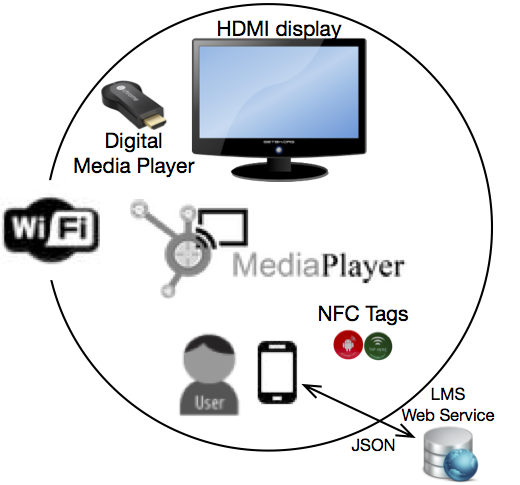
\includegraphics[width=0.9\linewidth]{img/nfcreview_fig2}
     \caption{NFC MediaPlayer�s ecology of resources}
     \label{fig:2}
\end{figure}
\subsubsection{Implementation}
The NFC MediaPlayer has been released in January 2015 as part of a larger research aiming to provide ubiquitous support for lifelong learning with mobile technology. The source code of this tool is available\footnote{NFC MediaPlayer open source code repository: https://code.google.com/p/lifelong-learning-hub/source/checkout?repo=mediaplayer} under an open license\footnote{Licensed under the Apache License, Version 2.0. http://www.apache.org/licenses/LICENSE-2.0} to facilitate customization and extension to further learning environments, communities, etc. 

This section describes the tools that conform the ecology (See figure \ref{fig:2}):
\paragraph{Digital media player}
In the very last months, WI-FI enabled digital media players have arrived to the market: Google Chromecast\footnote{Google Chromecast. http://www.google.com/intl/en/chrome/devices/chromecast/} (July 2013), Roku\footnote{Roku streaming stick. http://www.roku.com/products/streaming-stick} (March 2013); Apple TV\footnote{Apple TV streamcater http://www.apple.com/appletv/} (January 2013). These devices broadcast audio and video content on a High-Definition display by direct streaming via WI-FI from the Internet. These devices stream multimedia content based on the commands (Play, Pause \& Stop) triggered from another networked device (i.e. laptop, tablet, mobile). The basic operation is that using your personal device as a remote and selecting the desired multimedia, the content is automatically broadcasted in the HDMI display where the digital media player is plugged. The ecology presented in this manuscript has been developed for Google Chromecast\footnote{Google Cast SDK. https://developers.google.com/cast/docs/reference/}.
\begin{figure}
     \centering
     
\includegraphics[width=0.9\linewidth]{img/nfcreview_fig3}
     \caption{NFC MediaPlayer. JSON file playlist}
     \label{fig:3}
\end{figure}
\paragraph{HDMI displays}
HDMI displays facilitate the visualization of videos independently of the dimension for which they were designed. When streaming video from the digital media player, the audio volume is controlled from the remote of the HDMI display and not from the client device (mobile device, tablet or laptop). This feature makes the interaction much more natural and integrated within daily life environment.
\paragraph{NFC enabled smartphone}
The mobile phone plays the role of a remote communicating with all the previous elements in the ecology. A NFC-enabled smartphone is able to decode the command recorded in the tag (NDEF message), and trigger the action pre-mapped for that action. 
\paragraph{NFC MediaPlayer app}
The NFC MediaPlayer app has been developed and released\footnote{NFC MediaPlayer in Google Play. https://play.google.com/store/apps/details?id=org.ounl.lifelonglearninghub.mediaplayer} for Android mobile phones in January 2015 (Beta version). When the app starts, the JSON file (Figure \ref{fig:3}) containing the information describing the list of videos to be presented in the playlist, namely, title, subtitle, author, thumbnail images, and the URL where the video is stored, is requested to a remote webservice. 
\begin{figure}
     \centering
     
\includegraphics[width=0.9\linewidth]{img/nfcreview_fig4}
     \caption{NFC MediaPlayer�s playlist}
     \label{fig:4}
\end{figure}
The interface navigation within the app has two screens:
\begin{enumerate}
\item Playlist screen (See Figure \ref{fig:4}b). The home screen of the app. Lists the information describing the videos that can be streamcasted. When a video in the list is clicked, the cast screen with the selected video is displayed.
\item Cast screen (Figure \ref{fig:5}b). Displays the information of the video selected in the list. The video starts when the play button starts or stops when in the pause button is clicked. The video can be moved forward or backward using the slider. The video is streamcasted to the HDMI Display depending on whether the Chromecast icon on the top right corner is selected or not.
\end{enumerate}
\begin{figure}
     \centering
     
\includegraphics[width=0.9\linewidth]{img/nfcreview_fig5}
     \caption{NFC MediaPlayer�s casting}
     \label{fig:5}
\end{figure}
\paragraph{Programmable NFC Tags}
This ecology includes five tags configured to trigger the following actions:
\begin{itemize}
\item Positioning. The 1)\em positioning \em tag is configured to work in the playlist screen (Figure \ref{fig:4}b). When this tag is tapped (middle bottom tag in the whiteboard on figure \ref{fig:4}a/\ref{fig:5}a), the focus advances in the playlist marking in orange colour the active item.
\item Video casting. The 2)\em play \em and 3)\em pause \em tags are configured to work in the cast screen (Figure \ref{fig:5}b). When the play tag is tapped (left middle tag in the whiteboard on figure \ref{fig:4}a/\ref{fig:5}a), the active video is streamcasted to the HDMI display. The video is paused when the pause tag (right middle tag in the whiteboard) is tapped.
\item Navigation. The 4)\em playlist \em and 5)\em cast \em tags are configured to navigate between the playlist screen (figure \ref{fig:4}b) and the cast screen (Figure \ref{fig:5}b). When the playlist tag is tapped (left top tag in the whiteboard) the app presents the playlist screen. When the cast tag is tapped (right top tag in the whiteboard) the app presents the cast screen.
\end{itemize}
\section{Discussion and Conclusions}
This manuscript proposes the use of NFC technology towards the harmonization between digital and physical worlds for learning.

The literature review presents daily life scenarios (formal education settings, workplaces, museums, guided tours, fieldtrips, life-logging, smart home, simulations, logistics) where NFC technology has been previously used. Findings in the literature review reveal the increasing use of NFC-mobile devices for reading tags, in contrast to external reader. This fact is probably strengthen by the proliferation of NFC-enabled mobile devices and the increasing adoption of NFC technology in the last years \citep{Bialke2014}. The review shows that using mobile devices to drop (write content) on tags is not a developed practice yet in contrast to reading content that is the most popular use. 

On the other hand, this manuscript highlights the potential of NFC technology to facilitate the scaffolding of personal learning environments binding learning activities to daily physical spaces. The \em NFC MediaPlayer \em is presented as a real instantiation of ecology of resources in a frequent lifelong learning environment tackling three barriers:
\begin{enumerate}
\item Time. Reducing the time to start a learning activity.
\item Interaction. Reducing the number of clicks to access the learning content to zero clicks.
\item Visualization. Streamcasting video learning contents in a High-Definition quality in contrast to small-sized screens like mobiles, tablet or laptops.
\end{enumerate}
This ecology increases the chances of learning in scattered moments (i.e. waiting times, commercial break on TV) replacing this perceived "lost time� into perceived "productive time". 

In future research, we will scaffold ecologies to provide effective feedback services for learning (i.e. ambient displays, recommendations, analytics) and to foster meta-cognitive skills \cite{Tabuenca2014}. 







		%\clearpage{\pagestyle{empty}\cleardoublepage}	
		\addtocontents{toc}{\protect\newpage}
		
	\part{Formative studies and prototypes}
		\chapter{Where is my time? Identifying productive time of lifelong learners for effective feedback services}

\vfill
Lifelong learners are confronted with a broad range of activities they have to manage every day. Hence, learning activities from lifelong learners are disrupted. The difficulty to find a suitable time slot to learn during the day has been identified as the most frequent cause. In this scenario mobile technologies play an important role since they can track suitable moments to accomplish specific learning activities in context. Sampling of learning preferences on mobile devices are key benchmarks for lifelong learners to become aware on which learning task suits in which context, set realistic goals and set aside time to learn on a regular basis. The contribution of this chapter is twofold: first, a classification framework for modelling lifelong learners� preferences is presented; second, a mobile application for sampling of experiences is piloted aiming to identify which are the preferences from lifelong learners regarding \textit{when}, \textit{how} and \textit{where} learning activities can be integrated.
\vspace{3em}

This chapter is published as: 

Tabuenca, B., Kalz, M., B�rner, D., Ternier, S., \& Specht, M. (2014). Where is my time? Identifying productive time of lifelong learners for effective feedback services.In \textit{Communications in Computer and Information Science}. In Computer Assisted Assessment. Research into E-Assessment (pp. 149-161). Springer International Publishing.
\clearpage

\section{Introduction}
Choosing time and learning opportunities effectively is one of the major challenges for lifelong learners as confirmed by recent statistics \citep{Eurostat2012}. This survey shows that the participation in lifelong learning activities in Europe decreased between 2006 and 2011. Participants in this survey mention access, time, place, and lack of personalization as barriers to accomplish learning activities. Kalz stresses the importance of supporting self-direction and self-organization of lifelong learners with regard to using new technologies \citep{Kalz2014}. Lifelong learners face the challenge to combine their professional activities with learning activities and engage simultaneously with family times to ensure a balance of adults� responsibilities, overall wellbeing and their personal development. However, finding an appropriate balance between different life domains is neither easy nor instantaneous \citep{Metzger2004}. We have recently conducted a study in which lifelong learners reported that their learning experiences are disrupted, arguing the difficulty to find a suitable time slot to learn during the day as the most frequently reported reason by the participants \citep{Tabuenca2013}. Moreover, learners highlighted the importance of smartphones to support more constant learning experiences. Hence, there is a need to integrate learning activities in daily life. The \cite{EuropeanCommission2007} enumerates eight key competences that are fundamental for each individual in a lifelong learning society. One of them is \textit{learning to learn}, i.e. the ability to organize one�s own learning through effective management of time and information, and becoming aware of one�s learning. 

Providing in-context support and feedback for lifelong learners is key to identify the best learning moments, identify available resources in each context, self-organize their learning day, and set realistic goals. Lifelong learning not only implies setting aside regular time for learning during the day, but also combining learning activities with daily life activities. Mobile devices can facilitate users to track learning preferences in context \citep{Tabuenca2012d}. \cite{Hattie2007b} state that effective feedback answers three questions: \textit{where am I going?} , \textit{how am I going?} and \textit{where to next?}. To provide support for lifelong learners we are currently developing mobile tools and services to provide feed forward feedback (answering the question \textit{Where to next?}) targeting the process and self-regulation level. 

As a method for the development and data collection we have chosen the Experience Sampling Method (ESM \citep{Hektner2007}. Sampling of learning experiences in context provide an important benchmark for lifelong learners to identify productive times during the day and to scaffold their learning day on top of these moments. ESM is a psychological method that asks participants to stop at certain times and make notes of their experience in real time, gathering direct and contextual objective measures and situated subjective measures. A good portion of ESM research has been done exploring both the structure of classrooms as well as students� and teachers� subjective experience in them, by linking variations in attention, interest or challenge to specific instructional practices or conditions \citep{Leone1989,Crocker2003}. Likewise, contextual ESM has been used to understand daily information needs of people in longitudinal studies \citep{Church2014}. ESM responses measure what the person decides to communicate about his inner states whenever he is prompted a question. It is well known that we tend to be biased and edit out responses according to social desirability \citep{Hektner2007}. For instance, what does it mean if I score 4 in a 5-Likert scale on the question �\em how busy are you in this moment?\em  � where 1 corresponds to �very busy�? This measure can be quite different depending on the habits or culture of the person who answers. Nevertheless, these reports are significantly more powerful and accurate when they are self-reports (since I only take myself as a reference to measure how busy I am in this moment).  Hence, ESM facilitates an intimate and exhaustive account on how people go about their daily existence \citep{Hektner2007}. Mobile technologies provide an interesting opportunity for users to evaluate situations based on �stimulus variables in the natural or customary habitat of an individual� \citep{Hormuth1986} since they are reported in our own personal device. 

This chapter presents a classification framework that aims to support lifelong learners in their need to model the learning day by instantiating different variations of the ESM. Furthermore, results from a small-scale pilot study are presented to collect experiences and feedback about the chosen approach, the type of the preferred notifications received, and their preferred format when sampling the experiences on a mobile device.

\section{A classification framework for sampling of experiences using mobile devices}
In 2003, \cite{Consolvo2003d} explored the use of the ESM to evaluate regular phones, PDAs, paper booklets or audio recorders (�\em ubicomp applications\em �). This evaluation concludes that every instance of the ESM is dispatched in three sequential events (see figure \ref{fig:Esm_fig1}): 1) receive a notification; 2) dispatch the question (read, listen, watch); 3) provide an answer.

Nowadays, smartphones are equipped with several sensors that enrich the quality and quantity of the sample with contextual information. Mobile devices enable capturing different context variables and can identify the users� location (GPS), orientation (digital compass), among others. In a first analysis for distinguishing the role of context in mobile learning support, \cite{Jong2008d} have identified the main dimensions of context information used in learning applications and further extended to the context taxonomy to the Ambient Information CHannEls model (AICHE) meta-information \citep{Specht2009}. The AICHE model addresses context via sensors, artefacts and channels. This model approaches the context of a person or an object defined by five distinct dimensions (time, location, environment, relation and artefact identifier).

The classification framework presented in this section \ref{fig:Esm_fig1} merges ESM and AICHE models to provide specific cues on how can lifelong learners model their learning day. This framework instantiates the ESM to explore the dimensions of mobile context making use of the features provided by mobile devices in each of the sequential events in the instantiation of the ESM.

\begin{figure}[ht]
  \begin{adjustbox}{
  	addcode={
  		\begin{minipage}{\width}}{
	  		\caption{Classification framework for sampling experiences using mobile devices}\label{fig:Esm_fig1}
		\end{minipage}},rotate=90,center}
      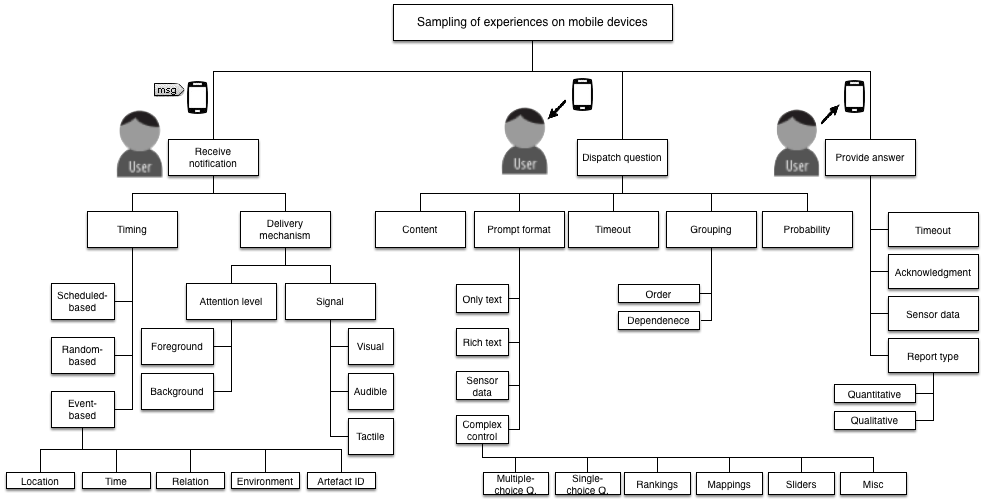
\includegraphics[scale=.6]{img/Esm_fig1}
  \end{adjustbox}
\end{figure}

\subsection{Receive notification}
Notifications can be classified according to two different criteria, i.e. time and delivery mechanism:

\textbf{Trigger time}, is the rule that identifies the moment in which the user receives the notifications. These notifications can be triggered on three different basis:

\begin{itemize}
\item Scheduled-based: Notifications are triggered following a time pattern, e.g.\em send me a notification every Sunday at 8pm asking me what was the best moment to read during the week\em .
\item Random-based: Notifications are triggered randomly in time, i.e. not following any time pattern, e.g.\em send me 5 notifications per day asking me how do I feel in that moment\em . This type of alerts can be used to identify best occasional learning moments. The fact of randomizing notifications is not only referred to the timing, but also randomizing the number of alerts sent, or randomizing the order in which a sequence is sent.
\item Event-based: Notifications are triggered on the accomplishment of an event that happened in the context of the user. Hereby, the dimensions of mobile context are explored with the aim to identify ways to support lifelong learners in their goal to organize their own learning towards effective context adaptation:

i) Location. Mobile devices are equipped with capabilities (e.g. GPS or Bluetooth) that make them aware of the current location of the user, e.g.\em send me a notification every time I arrive to the University in order to ask me what do I expect to learn today\em . Sampling this experience might foster lifelong learner�s capacity of reflection to set reasonable goals before starting the learning day \citep{Tabuenca2012d}. 

ii) Artefact identification. Mobile devices are equipped with capabilities (e.g. Near Field Communication readers or Quick Response code reader) that enable them to identify tagged artefacts in learner�s context. E.g.\em every time I approach with my mobile device the (NFC) tag attached to my German grammar book, send me a notification asking me how many pages did I read today\em . Sampling this experience might help the lifelong learner to track his pace of reading while learning the German language and set aside time to learn on a regular basis.

iii) Time. Mobile devices provide calendar functionalities that facilitate the configuration of notifications triggered on the accomplishment of time conditions. E.g.\em two weeks before I have an exam-appointment in my calendar, send me a notification asking me to rate from 0 to 10 how prepared I am for the exam\em . Sampling this experience might help the lifelong learner to monitor his perceived knowledge on a subject, and make a plan to prepare the exam with enough time.

iv) Relation. This dimension captures the relation an entity has established to other entities, and describes social, functional and compositional relationships. Mobile devices are equipped with capabilities (e.g. social network apps, messaging) that enable them to identify and/or cluster in groups other entities, and the type of connection they have with the lifelong learner. E.g.\em every time my colleagues are online in the campus social network, send me a notification to ask me whether I had any problem making my homework\em . Sampling this experience might help the lifelong learner to identify drawbacks accomplishing learning activities, and provide direct cues of support to existing drawbacks.

v) Environment. This dimension captures tasks and actions happening in the environment. Mobile devices are equipped with sensors (e.g. compass, GPS) and apps (e.g. forecasting weather or traffic jam) that make them aware of the context in the environment of the user. E.g.\em send me a notification when the weather forecast for the weekend is rainy so I can borrow a book from the library and stay at home\em . Sampling this experience might help the lifelong learner to model his week based on the conditions of the environment.
\end{itemize}

\textbf{Delivery mechanism}. Notifications can happen in the background, when the notification can be dispatched in a different context in which the notification is received. Nevertheless, ESM notifications must happen in the forefront so the sample can capture the specific lifelong learning context when/where they are received. Notifications in the forefront must call user�s attention. Mobile devices feature three main types of delivery mechanisms, namely, visual (e.g. icon, blinking light, adjust brightness, etc.), audible (e.g. beep, tone, etc.) or tactile (e.g. vibration). 

\subsection{Dispatch question}
There are different ways to prompt questions using mobile device. Hereby, we distinguish the following:
\textbf{Content}. The content of the messages can be designed with the purpose of alerting the student about the date of the exam, informing on the study-hours needed for the current week or reporting the grades. As cited before, \cite{Hattie2007b} state that effective feedback service must answer three questions: \textit{where am I going?}, \textit{how am I going?} and \textit{where to next?}. Probably the feedback will be more productive the more customised is to the receiver ( e.g. \textit{a suggestion from the teacher to improve my performance based on my grades}), rather than generic information ( e.g.\textit{Hei! today is a good day to learn!})

\textbf{Prompt format}. Questions can be formulated in different formats:
\begin{itemize}
\item Text. Text is the most compatible format across mobile device. They are not only implemented in regular mobile phones (e.g. SMS), but also in smartphones (e.g. chats, online questionnaires) or PDAs.
\item Rich text format. Rich text format is an extension of text prompts, but formatted with special font (type, size, colour etc.), images and/or multimedia (audio, video). These features need to be carefully combined so they do not impact the participant�s ability to read. 
\item Sensor data facilitates the enrichment of the questions with context data. E.g.\em  Today is a rainy day suitable to stay at home, do you feel like posting an entry in your sew blog?\em .
\item Complex control. Visual environments facilitate the implementation of prompts that aim to describe and collect complex concepts like relations, clusters, orders etc. Instances of complex controls are: 

i) Multiple/simple choice questions implemented with text and/or images. E.g.\em select which learning activity do you prefer to do while commuting to work by bus: (1)listen; (2)read; (3)write; (4)watch videos\em .

ii) Rankings facilitate ordering of items based on a specific criterion. E.g.\em based on your current priorities rank your learning goals for the coming month: learn German; iOS development; statistics; research methods\em ; 

iii) Mapping items facilitate matching of concepts from different groups. E.g.\em how much time did you set aside for learning this week? Match your time availability (commuting to work; after dinner) to your weekly learning goals (German grammar; C\# programming structures for iOS development)\em .

iv) Sliders facilitate collection of a specific value within a range of them. E.g.\em rate your overall progress of the week in statics towards your goal of being able to analyse data with ANOVA test (0 to 100\%)\em .

\end{itemize}

\textbf{Timeout} is the time that the question is available for the learner to be read. Most of the questions are only relevant when they are read within a specific range of time.

\textbf{Question design}. \cite{Consolvo2003d} described three variables when designing questions in ESM: order, i.e. whether the prompts� order should be fixed or random; dependency, i.e. whether a prompt is presented depending on what the user reported in a previous question (\em  e.g. every time I report low learning performance, trigger an instance asking me to report on my regular sport activity so I can see weather there is direct correlation\em ); probability, i.e. whether there is a need to assign probabilities that a question will be asked.

\subsection{Provide answer}
The answer refers to the externalization of learner�s experience in a mobile device. We distinguish the following components as relevant items for the classification framework.

\textbf{Timeout}. The time the user has to answer the question.

\textbf{Answer format}. Mobile devices today are equipped with text editors, audio and video recorders or photo camera. Likewise, the proliferation of apps to survey data (e.g. personal response systems, questionnaires) facilitate lifelong learners a wide range of input formats to record their experience. Lifelong learners not only learn by analysing the data answered in subsequent iterations of the ESM, it is also expectable that the single fact of externalizing an answer will trigger a different cognitive process depending on the format of the answer. For instance, reporting an answer with an audio-speech \citep{Nielsen2002} implies a different cognitive process than the one triggered by answering to a multiple-choice-question. Question and answer within an instance of the ESM do not necessarily need to have the same format. Answers reported in an ESM can be: 

\begin{itemize}
\item Quantitative. Refers to data that can be quantified in a specific number. Sliders, rankings, mappings and sensor data are instances of items to collect quantitative data. E.g.\em report how many hours did you invest this week on physical activities\em .
\item Qualitative. Refers to data aimed to collect descriptions, sensations, features or abstract characteristics. Open answers in text, audio or video recordings are instances of items to collect qualitative data. E.g.\em every time I pass an exam, record a power video to motivate you for the next one \em.
\end{itemize}

\textbf{Sensor data} facilitates the enrichment of the sample with context data so lifelong learner�s report can be correlated with variables that a mobile device can capture. E.g. \em every time I run and report a good performance, record the local temperature to find a correlation with weather conditions\em.

\textbf{Acknowledgment} checks can be used to indicate whether the question was read or an answer was given.

\section{Qualitative study}
\subsection{Introduction}
The qualitative study presented in this section instantiates the framework of the previous section with the aim to make participants aware of their learning preferences, and evaluate which type of questions and answers do they find more suitable in their context. This study took place in a workshop at the Joint European Summer School on Technology Enhanced Learning 2013 (JTELSS 2013) in Limassol (Cyprus). This event offers a learning environment where participants get opportunities to develop research skills, increase their knowledge base, engage in debate, have access to experts in the field, and discuss their own work.

A hands-on workshop presented the ESM as a method of research in the field of lifelong learners, showed existing tools and piloted an app for sampling of experiences. This pilot was guided by the following research question:

RQ1: What are lifelong learner�s preferences, requirements, and needs for ubiquitous support? Including the following sub-questions:

\begin{enumerate}[(a)]
\item When do lifelong learners prefer to be alerted to report about learning preferences, requirements and needs?
\item How do lifelong learners prefer to be alerted to report about learning preferences, requirements and needs?
\item Which formats do lifelong learners find more suitable to report about learning preferences, requirements and needs?
\end{enumerate}

\subsection{Method}
\subsubsection{Participants}
The experiment involved 12 voluntary and non-rewarded participants. They were all researchers in the field of technology-enhanced learning, five of them were women and the average age was 29.
\subsubsection{Materials}
The ESM pilot was developed adapting an existing open-source tool for educators, researchers and learners: ARLearn \citep{Ternier2012} (Figure \ref{fig:Esm_fig3}). Two participants used their own mobile devices. The rest borrowed smartphones for the experiment.
\begin{center}
\begin{figure}[ht]
\centering
	\subfloat[List of items]{
		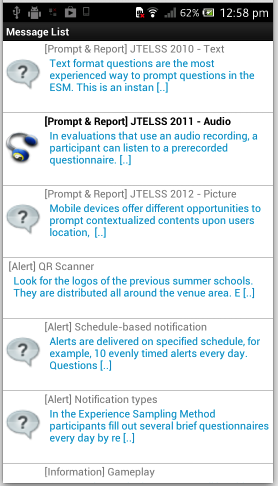
\includegraphics[width=0.3\linewidth]{img/Esm_fig3a}
		\label{fig:Esm_fig3a}
	}
	\subfloat[Question prompted in video and answer reported in video (qualitative report)]{
		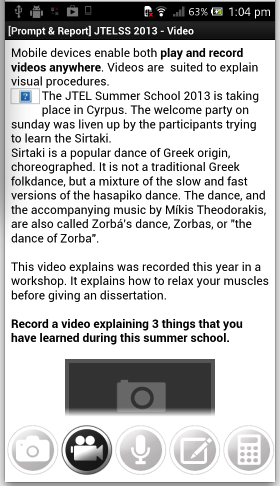
\includegraphics[width=0.3\linewidth]{img/Esm_fig3b}
		\label{fig:Esm_fig3b}
	}	
	\subfloat[Question prompted in text and reported in 5-Likert scale (quantitative report)]{
		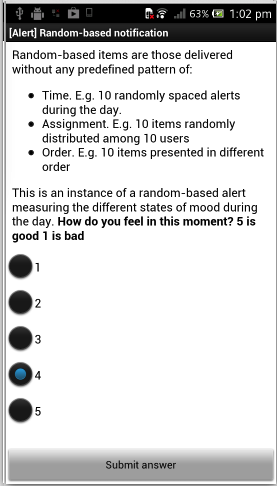
\includegraphics[width=0.3\linewidth]{img/Esm_fig3c}
		\label{fig:Esm_fig3c}
	}	
      \caption{ESM app}
     \label{fig:Esm_fig3}
\end{figure}
\end{center}
\subsubsection{Design}
All the participants in the experiment had the same treatment. This experiment took place during 90 minutes distributed in the following time slots:
\begin{itemize}
\item Lecture. 30 minutes introducing the ESM and showing theoretical framing of the workshop.
\item Field trip excursion sampling experiences. 40 minutes of practical experiment in which the participants followed the flow given in the mobile app as illustrated in figure \ref{fig:Esm_fig4}.
\item Questionnaire \& discussion. 20 minutes, brainstorming, feedback and data collection
\end{itemize}
A questionnaire gathered their learning preferences regarding mobile usage. Three questions were asking about their preferred sampling method and two about general appreciation of the app.

\subsubsection{Procedure}
The lecture presented the guidelines to perform sampling of experiences with mobile technologies.  The app whose flow is illustrated in figure \ref{fig:Esm_fig3} was designed so the participants could experience the different type of notifications that can be triggered when implementing the ESM, namely, scheduled-based notifications, event-based notification and random-based notifications. The flow comprised the following items presented to the participants in the form of notifications:
\begin{itemize}
\item App instruction items (See single-lined squares in figure \ref{fig:Esm_fig3}). These items teach them how to navigate within the app, how to record audio, etc.
\item ESM instruction items (See double-lined in figure \ref{fig:Esm_fig3}). These items were instances of the ESM in the form of notifications appearing in their incoming message box on the following bases: scheduled-based notification came two minutes after starting the app; event-based notifications came after scanning QR codes around the venue (Figure \ref{fig:Esm_fig3a}) and, after reading the scheduled-based notification (see dependencies in classification framework); random-based notification came in some moment after the first notification. For these items, participants should read the question given in text, rich-text (Figures \ref{fig:Esm_fig3b} and \ref{fig:Esm_fig3c}), audio, or video (Figure \ref{fig:Esm_fig3b}). After that, they should answer in a required format that could be text, audio, video (Figure \ref{fig:Esm_fig3b}), picture or likert scale (Figure \ref{fig:Esm_fig3c}).
\end{itemize}
\begin{figure}
     \centering
     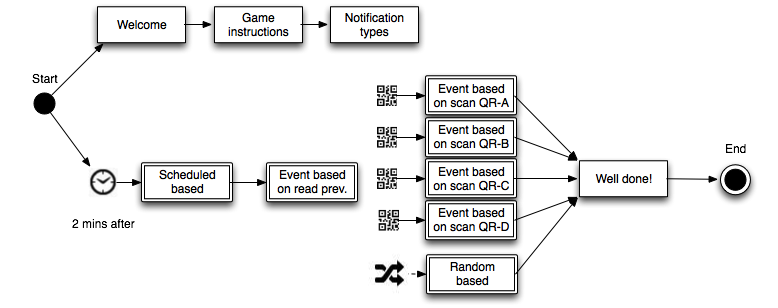
\includegraphics[width=0.9\linewidth]{img/Esm_fig4}
     \caption{Flow of the ESM app}
     \label{fig:Esm_fig4}
\end{figure}

\subsection{Results}
\begin{figure}
     \centering
     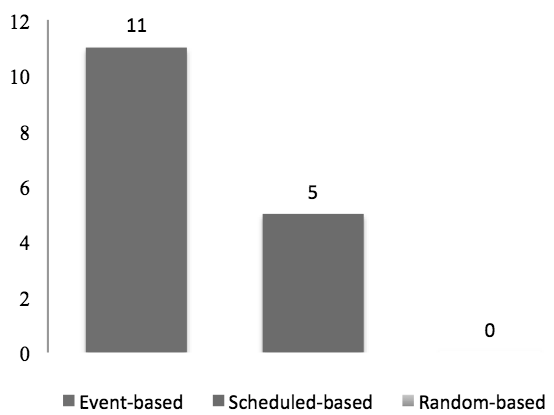
\includegraphics[width=0.5\linewidth]{img/Esm_fig5}
     \caption{Timing preference for notifications prompted on mobile devices}
     \label{fig:Esm_fig5}
\end{figure}
When participants were asked when they preferred to be notified to report about learning preferences, requirements and needs, event-based notifications were preferred by 92\%, scheduled-based by 42\% and random-based by 0\% of the participants (Figure \ref{fig:Esm_fig5}). Participant 1 (P1) preferred �event-based� and �scheduled-based� arguing that these types of notifications are �\em  Easier to organize as a learner\em �. Some of the participants raised compatibility working aspects in �scheduled-based� notifications. P4: �\em scheduled-based alerts would fit more my working preferences\em �. One participant highlighted the bias effect of expecting a question, happened especially in �event-based� notifications, but also in �scheduled-based� notifications. P3: �\em It was logical to expect a question after a particular event\em �. As event-based items were triggered by scanning QR codes attached to physical objects, some participants raised the proximity of attaching digital information to physical world objects. P5: �\em Information shown in event-based event seemed to be closer to me\em �. P6: �\em event-based notifications are more relevant since they are triggered as a consequence that something in my environment was happening\em �. 

When participants were asked how they preferred to be alerted to report about their learning preferences, requirements and needs, the majority of the participants preferred texts and picture formats (Figure \ref{fig:Esm_fig6}). Participants that selected �text� and �picture� argued focus on the information and accuracy on the explanation. P1: �\em You get more focused info and it is easier to understand the question\em �. Intrusiveness aspects were detected for participants that preferred text. P2: �\em It is the least intrusive way\em �. Some participants raised the usefulness of making knowledge understandable to someone and express their impressions with video and picture formats. P3: �\em Pictures and videos convey a lot of knowledge in relatively short time\em �. Context or environment, were raised as key elements to decide the suitability of the notification, to the extent that some participants did not report a concrete preference. P4: �\em They are all useful media formats depending on the context\em �. Suitability of the format text was preferred because of its facility to adapt to be read in different contexts. P5: �\em I can easily adapt my time to read in a suitable moment\em �. P6: �\em Text and pictures are better to describe an understanding\em �. P8 preferred text and argued �\em The rest of the formats are a kind of �invasive� mode of communication that might not adapt to the different times of the day, night\em�. Pictures and videos were reported as more �catchy� (P9). P10 reported text preference arguing that they are less distracting than the rest o the media. When this is about recording feelings and emotions, audios facilitate it. P12 preferred audios arguing �\em personal audio recordings facilitate it in a more personal way\em �.

When lifelong learners were asked which formats they find more suitable to report about learning preferences, requirements and needs, the majority of the participants reported pictures and text as preferred formats (Figure \ref{fig:Esm_fig6}). Rapidity on creating the answer was argued as key aspect by some participants. P1: �\em It is faster\em �. Likewise as happened in previous question, some participants raised the usefulness of making knowledge understandable to someone and express their impressions with video and picture formats. P3: �\em Pictures are easy to take and again convey a lot of data\em �. Participants seemed to be more used to text messaging. Some participants raised were more familiar reporting text samples. P3: �\em Text is the simplest way\em �. One participant highlighted that videos are well suited recording of procedures. P4: �\em Video answers facilitate explaining a flow of information\em �. Audio recordings were perceived as more natural interventions when reporting. P5: �\em Audio recording is a more natural interaction interface\em �. Pictures seem to be really popular and easy to report method. P5: �\em Taking pictures is a pretty common way to report with a mobile phone\em �. Some participants discarded the use of text of notifications because of the difficulty of writing long text messages on the small keyboards of smartphones. Even more remarkable when the smartphones are borrow and they are not the personal ones. P8: �\em Audios, pictures and videos are easier and faster to use\em �. P9: �\em I am more used to text and pictures\em �. P10 preferred picture reminding that �\em A picture is worth a thousand words\em �. Some consider pictures as easier to assimilate information. P11: �\em Text content is easier to process for me\em �. Videos are well suited to analyze the participant, gestures, or physical reactions when reporting. P12: �\em They are more indicative to see what you like to know from the participant\em �.

\begin{center}
\begin{figure}[ht]
\centering
	\subfloat[To read prompts on mobile devices]{
		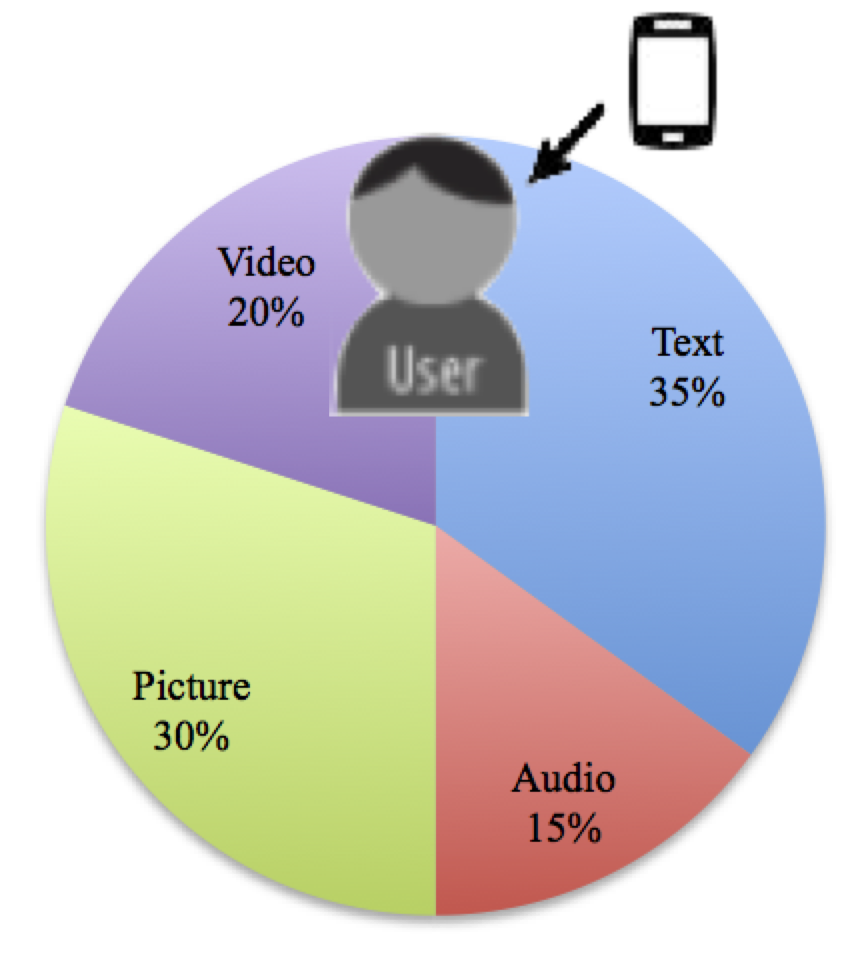
\includegraphics[width=0.4\linewidth]{img/Esm_fig6a}
		\label{fig:Esm_fig6a}
	}
	\subfloat[To report answers on mobile devices]{
		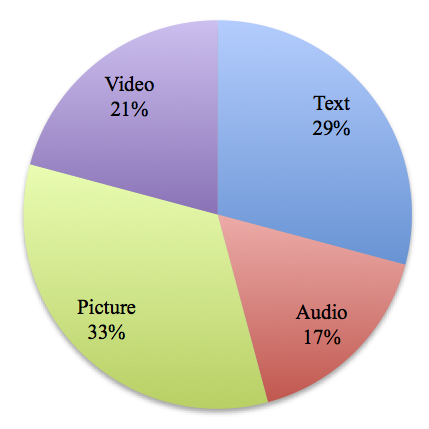
\includegraphics[width=0.4\linewidth]{img/Esm_fig6b}
		\label{fig:Esm_fig6b}
	}	
      \caption{Formatting preferences}
      \label{fig:Esm_fig6}
\end{figure}
\end{center}

\section{Discussion and conclusions}
\cite{EuropeanCommission2007} highlights the ability to organize one�s own learning through effective management of time and information, and becoming aware of one�s learning (�learning to learn�), as one of the eight key competences for each individual in a lifelong learning society. This chapter presents a suitable approach for introspection and modelling the learning day in lifelong learners. Instantiations of the ESM in personal mobile devices are proposed to foster awareness and to facilitate an intimate and exhaustive data collection on learning habits in context.

Recent work \citep{Gros2010} reviews time preferences and availability in e-learning classrooms across a 10-year period in scientific literature concluding that almost all the papers dealt with formal education and quantitatively oriented. The classification framework presented in the current chapter extends the walls of the classroom in lifelong learners to the mobile context, and proposes a suitable scaffold to identify productive moments exploring not only the quality and quantity of the time, but also the rest of the dimensions in the mobile context (location, relation, environment, artefact) \citep{Specht2009}. 

Moreover, this classification framework is instantiated in a study where a mobile app is piloted with the aim to make lifelong learners record and reflect on qualitative and quantitative learning preferences through the use of different features in smart phones. The experiment resulted in a successful experience in which participants were able to report their learning preferences in the specific context of a technology-enhanced learning summer school.

The work presented in this chapter represents an interesting technique for lifelong learners to get actively involved in knowing their own learning day. The ESM instantiated in personal mobile devices is very suited for lifelong learners to explore their own specific context, learning style, and available resources to model each learning moment.

This pilot has raised the following limitations: first, this pilot was tested at the venue of a summer school, which is an exceptional learning context. Real lifelong learning scenarios imply daily routines like workplaces, transitions, etc.; second, the duration of the experiment was too short. Modelling one�s lifelong learning day implies a long-term experiment in which moments of the day and moments of the week are explored. The analysis on work time and learning activities from \cite{Livingstone2007}, stresses the lack of longitudinal studies especially in job-related informal learning. Likewise, they highlight that initiatives to achieve better work-family balance are most likely to have a positive effect on either quality of work life or workers� learning opportunities, if the full extent of these long hours is recognized more clearly.

Mobile tools are increasingly used for sampling of experiences \citep{Church2014,Intille2003,Conner2013} in the last years in which different reports have reviewed existing tools for sampling of experiences \citep{Conner2013,Khan2009} classifying them by operating system (iOS, Android, etc.), the price of the app, the project where it was used, or the URL where it can be downloaded. Nevertheless, there is no scientific work reviewing existing apps featuring experience sampling on mobile devices. In future research, we will extend this work by providing a review of apps for ESM classifying the in accordance to the framework presented in this chapter and with a special focus on the use of ESM for self-regulated learning. Likewise, this research will be further extended developing mobile tools and services to provide effective feed forward feedback targeting the process and self-regulation level.




	
		
\chapter{Mobile authoring of OER for authentic learning scenarios}


\vfill
Learning resources are traditionally designed in desktop-based authoring systems where the context is mostly restricted to the learning objective, capturing relevant case characteristics, or virtual situation models. Mobile authoring tools enable learners and teachers to foster universal access to educational resources not only providing channels to share, remix or re-contextualize these, but also capturing the context in-situ and in-time. As a further matter, authoring educational resources in a mobile context is an authentic experience where authors can link learning with their own daily life activities and reflections. The contribution of this chapter is threefold: first, the main barriers for ubiquitous and mobile authoring of educational resources are identified; second, recent research on mobile authoring tools is reviewed, and 10 key shortcomings of current approaches are identified; third, the design of a mobile environment to author educational resources (\em MAT for ARLearn \em) is presented, and the results of an evaluation of usability and hedonic quality are presented.
\vspace{3em}

This chapter is published as: 
Tabuenca, B., Kalz, M., Ternier, S., \& Specht, M. (2014). Mobile authoring of open educational resources for authentic learning scenarios. \em Universal Access in the Information Society\em . Special Issue: The Use of Mobile Technology and Ubiquitous Computing for Universal Access in Online Education), 1�15. doi:10.1007/s10209-014-0391-y

\clearpage

\section{Introduction}
\label{sect:1}
Situated learning \citep{Brown1989} stress the importance of knowledge and skill acquisition in the same context in which they need to be performed; leading also to the concept of communities of practice \citep{Lave1991}. While some educational media simulate real world environments with 3D-visualizations or micro-worlds several authors have stressed the difference between a simulated environment and authentic experiences in the real world \citep{Hummel1993, Tripp1993}. \cite{Rule2006} clusters authentic learning into four themes: (1) real-world problems that engage learners in the work of professionals; (2) inquiry activities that practice thinking skills and metacognition; (3) discourse among a community of learners and (4) student empowerment through choice. The seminal article from  \cite{Herrington2000} identifies a number of design guidelines for situated learning activities like the need to provide authentic tasks and problems as also to support the change of perspectives. 

With the availability of mobile technologies new potentials for the design and creation of authentic and situated learning materials have emerged \citep{Duval2009}. Lombardi and Oblinger \cite{Lombardi2007} identify mobile devices as one of the key technologies to support authentic learning with information access and data collection during field-based investigations. On the one hand, learning support with mobile devices has increased access to advanced learning opportunities. On the other hand, the creation of learning materials in context, and the documentation of authentic learning experiences have been researched. Nevertheless there are still many restrictions for the authoring support of authentic learning resources on different aggregation levels. Several research projects have demonstrated the potential of using mobile and ubiquitous devices to capture contextual information \citep{Zimmermann2005d} and recording real-life experiences \citep{Barreau2007, Hodges2006} but this potential has remained underexploited for the process of mobile authoring of learning resources.

Within this chapter we refer to ''Mobile Authoring'' as the process of content creation on different levels of aggregation by using mobile technologies. \cite{Kinshuk2013} discuss the relevance of mobile authoring when capturing learning where and when it occurs. Additionally, they stress the lack of learner generated content in reusable learning objects authored for e-learning, especially with timely, relevant, and location aware examples. 
This chapter reports about an analysis of existing mobile authoring solutions and the development and evaluation of a new mobile authoring tool  for open educational resources. In the next section we report about related work and discuss shortcomings of current mobile authoring tools. In section 3 we introduce the Mobile Authoring Tool for ARLearn (\em MAT for ARLearn \em) that we have build aiming at authentic learning environments and the related authoring activities as also the shortcomings of analyzed tools. In section 4 we introduce an evaluation of usability and hedonic quality of the \em MAT for ARLearn \em. Section 5 discusses these results and limitations of the work. Last but not least we discuss future research.

\section{Motivation and related work}
\label{sect:2}
Authoring learning resources is currently still a process that is generally conducted in front of a desktop computer making it hard to capture real-life experiences related to the actual learning situation. Most of the current authoring environments are desktop solutions that enable the deployment of the authored learning materials to mobile devices \citep{Perez-Sanagustin2012a, Gruntjens2013, Sampson2012, Gicquel2011, Mathews2010, MartIn2009, Cabada2009, Kim2013}. In this scenario, the user authors an educational resource surrounded by blank walls and situated in front of a computer screen. Authoring educational resources in a mobile context is a more authentic activity that provides access to real-life experiences, which are otherwise not easy to capture. For instance, when creating a learning resource about the architectural design of a building in the physical environment and context in which the building is located, the created learning materials and documentation are expected to be very different from the materials designed on a desktop computer. The creation in-situ and perception of relevant affordances and details is expected to impact the design of instructional materials as also the learning resource selection. 

Remix and re-contexualization are key practices within the field of Open Educational Resources (OER). The combination of authentic learning scenarios and mobile authoring facilitates the connection between real-world locations and digital learning resources. Therefore the reuse and re-contextualization potential can be even larger than in traditional technology-enhanced learning scenarios. Nevertheless, different authors are skeptical on the assimilation and progress of remixing and re-contextualization practices from educators� side.\cite{Amiel2013} concludes that remixing learning resources is still not mainstream in education. \cite{Collis2003} report little success with bringing instructors close to an actual authoring process: ''instructors do not have the time, interest, or skills''. The proliferation of smartphones and the familiarization of new generations with mobile technology are bringing students and educators closer to an authentic and contextualized authoring process and to support reuse and remix of earlier developed resources. 

The work from \cite{Mugwanya2010} reviews mobile learning content authoring tools from 2002 to 2009. The authors categorize these tools according to technology used, pedagogy and usability dimensions. They summarize that the majority of the tools are developed with the goal of being integrated into Learning Management Systems (desktop computer) and stress the need to develop mobile authoring tools that empower users to author content for use in mobile environments. More recently, several authors \citep{Perez-Sanagustin2012a, Gruntjens2013, Sampson2012, Gicquel2011, Mathews2010, MartIn2009, Cabada2009, Kim2013} have proposed solutions for desktop-based authoring of mobile content. These studies report about functionalities like the preparation of routes in maps, the binding of content to QR codes, or language learning content created on mobile devices to be later deployed for mobile learning support. Nevertheless these learning contents are mostly authored in front of a computer screen outside of the real context in which the mobile learning intervention is conducted later.

In contrast to desktop-based authoring, we have conducted a review of existing tools that support the mobile authoring of learning resources. There are different models classifying learning resources according to their granularity \citep{Wagner2002, Duval2003a}. In the following, we will review mobile authoring tools aiming to shed light both on the granularity of mobile generated learning contents, and, what features do mobile authoring tools provide to foster universal access to existing learning resources. 

\subsection{Review in mobile authoring tools}
\label{sect:2_1}
The underlying search was conducted utilizing the online research repositories of the Association for Computing Machinery (ACM), the publisher Springer, Google Scholar, as well as the IEEE Computer Society. The focus on these repositories is reasonable as they cover a sufficiently large number of relevant publications. Within the ACM digital library an advanced search was performed in late January 2014 querying all articles of type journal, proceeding, or transaction that had been published since 2005 when mobile phones became more popular, and matching the keywords ''authoring AND mobile'' as part of the title. The query revealed 8 results whereof 4 were appropriate. As this query did not report enough results, a second search in the full-text matching the keywords ''authoring AND mobile AND learning'' was performed. The query revealed 1051 results where the first 30 occurrences ordered by relevance were selected. These 34 items were filtered by title and/or abstract. The rest of the repositories where analyzed analogously as illustrated in figure \ref{fig:mat_1} The 24 resulting articles were fully analyzed and desktop-based authoring tools were discarded. This review has resulted in eight authentic mobile authoring environments listed in the appendix B ''Authoring tools in mobile context''.
\begin{figure}
	\centering
     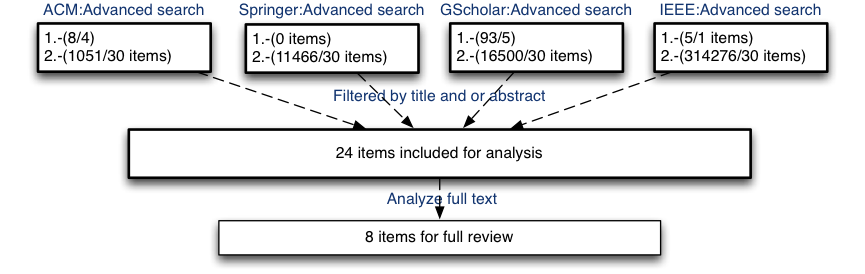
\includegraphics[width=0.9\linewidth]{img/mat_fig1}
	\caption{Mobile authoring tools review procedure}
	\label{fig:mat_1} 
\end{figure}
For a more in-depth analysis of the mobile authoring tools identified in the literature review we have compared the different granularity levels that they support in their authored educational resources. As a basis we have used modular content hierarchy from learning objects introduced by \cite{Duval2003a}. The result of this comparison is synthesized in table \ref{tbl:map1}.

\begin{sidewaystable}
  \centering
  \footnotesize
  \caption{Modular Content Hierarchy in mobile authored OER}
  \label{tbl:map1}

\begin{tabular}{lllllll}
\thickhline
\textbf{ } 	
	& \begin{tabular}[c]{@{}l@{}}Raw media \\ data elements \end{tabular}
	& \begin{tabular}[c]{@{}l@{}}Information \\ objects \end{tabular} 	
	& \begin{tabular}[c]{@{}l@{}}Application \\ objects \end{tabular} 
	& \begin{tabular}[c]{@{}l@{}}Aggregate \\ assemblies \end{tabular}  
	& \begin{tabular}[c]{@{}l@{}}Collection \end{tabular} \\ \thickhline
\textit{Mobile Author}	
	& Text 									
	& \begin{tabular}[c]{@{}l@{}}Multiple-choice question, \\ fill in the blanks \end{tabular} 												
	& \begin{tabular}[c]{@{}l@{}}List of questions \end{tabular} 							
	& - 									
	& -         \\ 
\textit{RAFT}			
	& \begin{tabular}[c]{@{}l@{}}Pictures, \\ annotations\end{tabular} 				
	& \begin{tabular}[c]{@{}l@{}}Learning objects \\ (aggregation of pictures, \\ annotations, \\ content metadata, \\ context metadata)	\end{tabular} 
	& - 										
	& - 									
	& -          \\ 
\textit{StoryKit}		
	& \begin{tabular}[c]{@{}l@{}}Pictures, \\ text, \\ drawings, \\ audio files \end{tabular} 
	& \begin{tabular}[c]{@{}l@{}}Page, i.e. text enriched \\ width multimedia \end{tabular} 													
	& \begin{tabular}[c]{@{}l@{}}Book/story, i.e. an \\ aggregation of pages \end{tabular} 		
	& \begin{tabular}[c]{@{}l@{}}Bookshelf, i.e. an \\ aggregation of books \end{tabular} 	
	& -          \\ 
\textit{MPAS}			
	& \begin{tabular}[c]{@{}l@{}}Image, \\ video, \\ text \end{tabular} 					
	& \begin{tabular}[c]{@{}l@{}}Multimedia \\ slides \end{tabular} 																					
	& \begin{tabular}[c]{@{}l@{}}Presentation, \\ aggregation of slides \end{tabular} 		
	& - 									
	& -          \\ 
\textit{MAAIMS}			
	& \begin{tabular}[c]{@{}l@{}}Audio, \\ video, \\ picture \end{tabular} 				
	& Learning object																					
	& - 										
	& - 									
	& -          \\ 
\textit{Quizzer}		
	& Text 									
	& \begin{tabular}[c]{@{}l@{}}Multiple-choice \\ question \end{tabular} 
	& Quiz 										
	& - 									
	& -          \\ 
\textit{mProducer}		
	& \begin{tabular}[c]{@{}l@{}}Video clips \end{tabular} 							
	& \begin{tabular}[c]{@{}l@{}}Learning objects, \\ i.e. aggregation of video \\ and context metadata	\end{tabular} 								
	& \begin{tabular}[c]{@{}l@{}}Stories \\(aggregation of \\ learning objects) \end{tabular}  
	& - 									
	& -          \\ 
\textit{MoVie}			
	& \begin{tabular}[c]{@{}l@{}}Video, \\ text \end{tabular} 							
	& \begin{tabular}[c]{@{}l@{}}Video clip \\objects	\end{tabular} 																			
	& \begin{tabular}[c]{@{}l@{}}Stories \\ (aggregation of videos) \end{tabular} 			
	& - 									
	& -          \\ \hline
\end{tabular}
   
\end{sidewaystable}


Resources that have a low granularity, such us \em raw media \em elements are highly reusable. \em Raw media \em elements include, pictures, text in the form of annotations, audios, video clips, metadata about content, metadata about standard (LOM, SCORM), or metadata about the context (GPS coordinates). \em Aggregate assemblies \em and \em collections \em have higher level of granularity but they are least reusable.

The content taxonomy presented in table \ref{tbl:map1} shows that all mobile authoring tools populate two to four levels of granularity. None of the mobile authoring tools populates the level of \em collection \em in the content taxonomy. This fact indicates that so far, content authored in mobile context is not created to be part of extensive collections, but rather to be integrated in units of lower granularity. An argument for this is the lack of available tools supporting remix of learning contents. 

The analysis of these articles has resulted in the identification of 10 limitations (L1-L10) of mobile authoring tools with regard to universal access of content authored in a mobile context:
\begin{enumerate}
\item Sharing functionality. Authoring tools must feature sharing of authored educational resources in order to foster reuse and facilitate the expansion. Only one of the presented tools allows the sharing of resources created via E-Mail (\em StoryKit\em).
\item Remix support: Remixing allows authors to reuse educational resources and their rearrangement within new application contexts. Only two of the analysed tools provide support to remix resources (\em Quizzer\em and \em Mobile Author\em). While the two tools only allow remix on the \em information object \em level, remix features should be provided on different granularity levels to exploit the full potential of sharing of learning resources.
\item Recontextualization: Recontextualization is the transfer of a learning resource from one context to the other. While related concepts like repurposing \citep{Rensing2005} focus on the change of educational context, for the mobile authoring of learning resources for authentic learning scenarios the re-contextualization from one location to the other is important. The tools \em MAAIMS\em, \em Quizzer\em, \em RAFT\em and Producer support this type of re-contextualization.
\item Editing: Editing of educational resources benefits the adaptation of contents, context, and the rearrangement of the learning objects. Mobile authoring tools should provide mechanisms to support edit of educational resources. Some tools feature edit of the content (\em StoryKit\em and \em Mobile Author\em). MMAIMS feature edit of content metadata, and others feature edit of context metadata (\em Quizzer\em and \em RAFT\em).
\item Search functionality: Mobile authoring tools should provide mechanisms to support allocation of educational resources from repositories \cite{Tabuenca2012c}. Search of educational resources should not only be indexed on the name, description or owner of the educational resource, but also, indexed on the dimensions of the mobile context \citep{Specht2009}, namely, location, time, environment, relation and artefact identification. Hence, mobile devices can facilitate context related search of OER based on the location, time of the day when the resource is useful, or depending on the people surrounding me in a specific moment.
\item Sharing license support: Licensing is an important feature when sharing and reusing mobile content. Recent case study \citep{Amiel2013} implementing remix of OER for language learning highlights the selection of suitable licences as key consideration: ''\em When remixing resources a series of considerations have to take place, which are not necessarily at the forefront in a traditional process of design. First off, one needs to be sure to select resources with more open licenses.\em '' Hence, the license model needs to support this remixing. Creative Commons has the right tools in place to flexibly support remixing of content. None of the presented tools (See appendix C) features any license assignment for authored content. 
\item Learning Object standard support: The implementation of Learning Object Metadata (LOM) standards facilitates content indexing and benefits the integration of OER across Learning Management Systems. Of the analysed tools three support the IMS LOM or SCORM standard: \em MAAIMS\em facilitates the creation of standardized learning objects (IMS Content Packages and standardized learning activities) whereas \em RAFT\em features SCORM.
\item Availability in open app markets: Mobile authoring tools should be available in open app markets as an approach to facilitate universal access to authoring tools. \em StoryKit\em is the only mobile authoring tool available in open markets.
\item Use of sensors: Some of the apps use different sensoring functionalities to support the contextualization and improve the quality of the learning resources. \em Quizzer\em uses the compass to serve content based on the orientation. In authoring mode, \em Quizzer\em records the orientation of the user to contextualize the resource. Moreover, \em Quizzer\em supports tagging of learning resources with the user�s identifier on creation time providing some control on the ownership of the resource. On the other hand, \em mProducer\em uses an accelerometer to measure the excessive amount of camera shaking recording a video, with the aim to filter blurry and unusable recordings. 
\item Interoperability. None of the tools reviewed facilitates the interoperability and exchange of educational resources among different mobile authoring tools.
\end{enumerate}

The above-presented summary shows that there is no ideal mobile authoring tool implementing all the necessary features to exploit universal access. While the availability in open app markets will be targeted at a later stage, we have taken the limitations revealed in the from the scientific literature review into the design of \em MAT for ARLearn \em.

\section{Design}
\label{sect:3}
\em MAT for ARLearn \em has been designed considering the limitations enumerated in the previous section. This tool aims to provide an open environment to facilitate any user (teacher or student) to author, share, edit, remix and recontextualize educational resources to foster universal access. Hereby we describe how \em MAT for ARLearn \em was designed and which of these shortcomings are covered.

\subsection{ARLearn: Cloud-based platform for mobile serious games}
\label{sect:3_1}
The Mobile Authoring Tool has been built upon ARLearn framework, an open source platform for authoring mobile serious games, available under the GNU Lesser GPL license \cite{Ternier2012}. ARLearn is accessible for the community as a cloud based solution where authors can, without cost, create content and deploy this content to mobile devices. Approx. 450 users have used the authoring environment to create games resulting in approx. 600 active games on the platform cloud. As illustrated in table \ref{tbl:map2}, learning resources in ARLearn are classified according to four different granularities in the model of content hierarchy \citep{Duval2003a}. We will further describe these objects providing some examples in the scientific literature where this platform has been used.
\begin{table}[h]
  \centering
  \footnotesize
  \caption{Granularity of learning resources in \em MAT for ARLearn \em}
  \label{tbl:map2}
  
\begin{tabular}{lllllll}
\thickhline
\textbf{ } 	
	& \begin{tabular}[c]{@{}l@{}}Raw media \\ data elements \end{tabular}
	& \begin{tabular}[c]{@{}l@{}}Information \\ objects \end{tabular} 	
	& \begin{tabular}[c]{@{}l@{}}Application \\ objects \end{tabular} 
	& \begin{tabular}[c]{@{}l@{}}Aggregate \\ assemblies \end{tabular}  
	& \begin{tabular}[c]{@{}l@{}}Collection \end{tabular} \\ \thickhline
\begin{tabular}[c]{@{}l@{}}MAT for \\ ARLearn \end{tabular}			
	& \begin{tabular}[c]{@{}l@{}}Pictures, \\ text, \\ drawings, \\ audio files \end{tabular}	
	& \begin{tabular}[c]{@{}l@{}}Audio item, \\ Video item, \\ Multiple-choice, \\ Text item \end{tabular}
	& \begin{tabular}[c]{@{}l@{}}Game\end{tabular}			
	& \begin{tabular}[c]{@{}l@{}}Set of games \end{tabular}	
	& -          \\ \hline
\end{tabular}
\end{table}

ARLearn was extended with an open repository where users can make games open, license it properly and share these with their peers. ARLearn has ben used in several authentic learning scenarios: 
\begin{itemize}
\item Recently, \cite{Schmitz2013} investigated role-playing on helping behavior with a mobile learning game to train basic life support and cardiopulmonary resuscitation. With this game they aimed at improving willingness to help in case of emergency (Figure \ref{fig:mat_2}).
\begin{center}
\begin{figure}[ht]
\centering
	\subfloat[Users had to allocate the defibrillator at the school and use it to save the victim.]{
		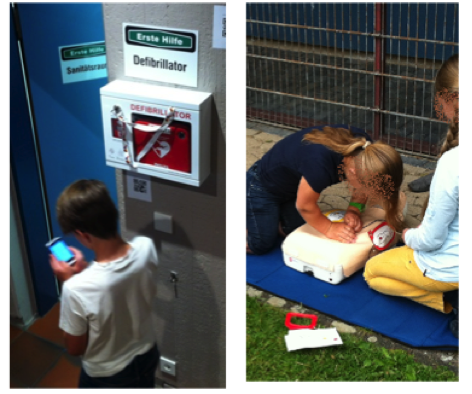
\includegraphics[width=0.5\linewidth]{img/mat_fig2a}
		\label{fig:mat_2a}
	}
	\subfloat[Users were instructed on the steps to follow in a cardiac arrest scenario. After the exercise, they were prompted to report the state of the victim.]{
		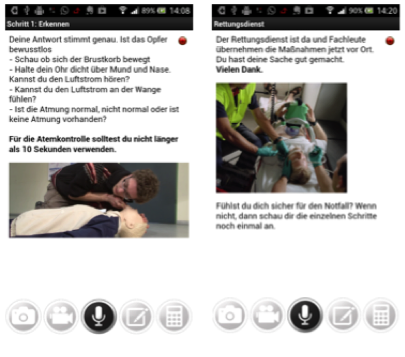
\includegraphics[width=0.5\linewidth]{img/mat_fig2b}
		\label{fig:mat_2b}
	}	
      \caption{Training cardiopulmonary resuscitation in schools with ARLearn \cite{Schmitz2013}.}
      \label{fig:mat_2}
	
\end{figure}
\end{center}
\item The Mindergie games have been designed and tested at a university campus in the context of an energy conservation pilot \citep{Borner2013a}. The goal of these games is to provide incentive mechanisms to decrease the energy consumption at the workplace. Every week players were given information, tasks and challenges, e.g. a video with hints on how to consume less electricity. 
\item In collaboration with the United Nations Refugee Agency \citep{Ternier2012z}, use cases for crisis situations were developed. These cases feature a social context through role-playing and typically zoom in on crisis situation like a hostage taking scenario. In this game employees are trained on how to react in such a situation. A game here is typically place in 5 phases: notification of the incident, assembling the team, planning, responding and negotiating. During the game players receive message according to their role. The head of office role will get a phone call from a journalist, while the staff welfare member needs to answer a call from a distressed family member.
\end{itemize}
The desktop-based\footnote{ARLearn desktop-based authoring environment. http://streetlearn.appspot.com/
} authoring environment for ARLearn (Figure \ref{fig:mat_3}) features the creation of games, teams, players, roles, items, and the dependencies among them. Moreover, it implements the Creative Commons (CC) licensing policy at the level of games (\em application objects \em) facilitating share and reuse across users. The games presented above are licensed under the CC attribution license. In the next section we describe the design and development of the \em MAT for ARLearn \em.
\begin{figure}
	\centering
     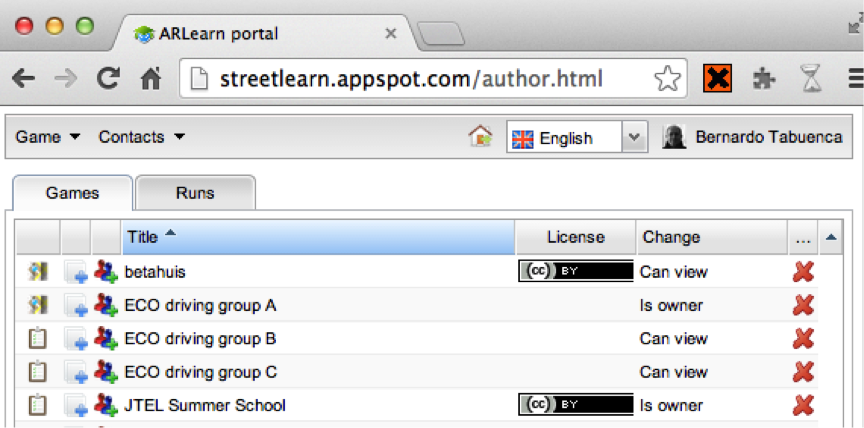
\includegraphics[width=0.9\linewidth]{img/mat_fig3}
	\caption{Desktop authoring environment in ARLearn}
	\label{fig:mat_3} 
\end{figure}

\subsection{\em Mobile Authoring Tool for ARLearn \em}
\label{sect:3_2}
The Mobile Authoring Tool complements the ARLearn desktop-based environment. Hence, a mobile game author can wander around creating items and synchronizing real world artefacts with game content. \em MAT for ARLearn \em has been designed starting a ''Mobile Authoring'' branch \footnote{\em MAT for ARLearn \em source code. https://code.google.com/p/arlearn/source/browse/?name=MobileAuthoring}  from the last release of the open source code available for the ARLearn mobile\footnote{ARLearn in Google Play. https://play.google.com/store/apps/details?id=org.celstec.arlearn2.android} client \citep{Ternier2012}. This procedure has facilitated the reuse of the already existent interfaces to access the backend via RESTful web services and the objects persisted in Google Appengine tables. The design of the tool has been performed adding functionality to the existing client following the next steps: first, we implemented the functionality to create a new game. Until now, it was only possible to create games from the desktop-authoring tool. These games are the containers of items; second, we implemented the functionality to create items so that users can create text items, video item, audio item and multiple-choice item in context recording or taking pictures with the mobile device; third, we perform the scientific literature review and identified the ten limitations for universal access; finally, these shortcomings were analysed and covered as illustrated in appendix C.

The \em MAT for ARLearn \em features three main approaches to foster ubiquitous and universal access to educational resources: 
\begin{enumerate}
\item an author can create and contextualize new content; 
\item an existing game (or an item) can be recontextualized to a new environment; 
\item licensing selection is supported to promote the reuse, revision, remixing, and, redistribution of educational materials as open educational resources (OER).
\end{enumerate}
 
The \em MAT for ARLearn \em features the ''My Games'' view as the starting point. Figure \ref{fig:mat_4a} shows the three games that the user authored for each of the architectural objects he is interested in; Figure \ref{fig:mat_4b} illustrates the ''Game View'' where the user can edit the resource and assign a licensing policy to share it. Clicking on the ''item tab'' (middle one) the user accesses the items that form this game. The author has the option to contextualize the content by binding it to the current coordinates, or by binding it to an existing QR code. Figure \ref{fig:mat_4c} illustrates the case of a user that has created a narrator item (text item) about the Church of St. Peter as an aggregation to the porticos \em Game\em (\em application object \em). As he is located in an authentic environment, for example in front of the church and staring at the portico, the description inspired on the real situation is completely different from the one he would create sited on his desk and watching a picture on the screen. As the user is in a mobile context, he can also contextualize the educational resource to the current location. In this case, the user can contextualize the item with the dimension \em location\em by registering the current coordinates and radius (See top of figure \ref{fig:mat_4c}) clicking on the ''Bind to location button''. The user can also contextualize the item with the dimension \em artifact identifier\em whenever there would be a QR code next to the church. By clicking on the ''Bind to tag'' button, he would scan the code and the educational resource would be attached to that physical object. Next, he can edit the resource to indicate the CC license that should be assigned to the item.
\begin{center}
\begin{figure}[ht]
\centering
	\subfloat["My games" screen lists games created by the author]{
		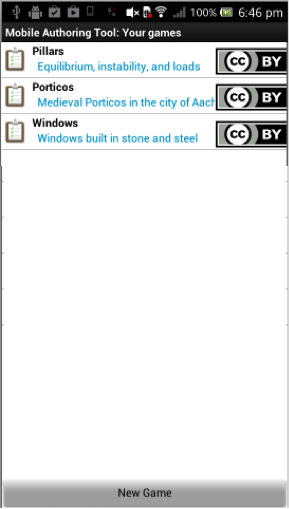
\includegraphics[width=0.3\linewidth]{img/mat_fig4a}
		\label{fig:mat_4a}
	}
	\subfloat[Authoring games screen]{
		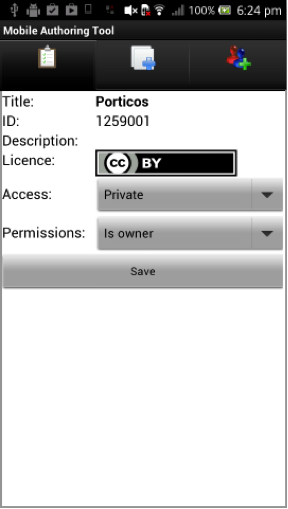
\includegraphics[width=0.3\linewidth]{img/mat_fig4b}
		\label{fig:mat_4b}
	}	
	\subfloat[Contextualization of educational resources]{
		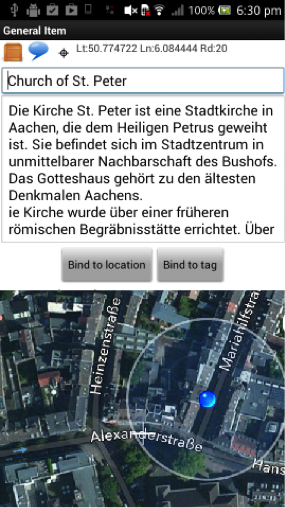
\includegraphics[width=0.3\linewidth]{img/mat_fig4c}
		\label{fig:mat_4c}
	}	
      \caption{Mobile Authoring Tool for ARLearn interface}
      \label{fig:mat_4}
	
\end{figure}
\end{center}
\subsection{OER remix in mobile context}
\label{sect:3_3}
Instead of creating a new resource from scratch the user can search already existing OERs to clone one and aggregate it without making any modification (remix), or, adapting it to the new context by updating any of the dimensions of the mobile context \citep{Specht2009} (recontextualizing). 

The \em MAT for ARLearn \em enables the user to issue a mobile OER search, to assess and to reuse an item in a new context. Users can also extend their game script by reusing a single item rather than reusing a game as a whole. Recontextualizing and remixing needs an infrastructure in place that supports flexible access to content. A search infrastructure must enable searching for content corresponding to different granularities. ARLearn supports searches from two granularities in the modular content hierarchy, namely, \em information objects \em (games), and \em application objects \em (items). Users can author games and items, and make them open access to the community. Figure \ref{fig:mat_5a} illustrates how licences are presented in descendent level of openness according to \citep{Vollmer2013}. Via this infrastructure, the \em MAT for ARLearn \em provides access to search functionality for items as well as for games as a whole when being in a specific context. 
\begin{center}
\begin{figure}[ht]
\centering
	\subfloat[Select level of openness for a new game]{
		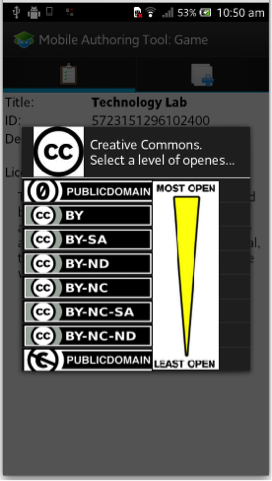
\includegraphics[width=0.3\linewidth]{img/mat_fig5a}
		\label{fig:mat_5a}
	}
	\subfloat[Search in already existing items for remix]{
		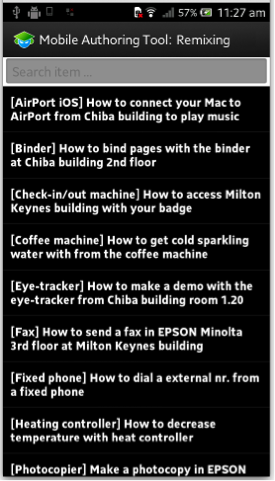
\includegraphics[width=0.3\linewidth]{img/mat_fig5b}
		\label{fig:mat_5b}
	}	
	\subfloat[Remix and recontextualization of a "text item" with location coordinates or artefact identifier ]{
		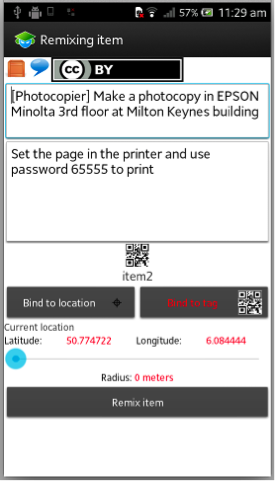
\includegraphics[width=0.3\linewidth]{img/mat_fig5c}
		\label{fig:mat_5c}
	}	
      \caption{Remixing and recontextualizing items with the \em MAT for ARLearn \em}
      \label{fig:mat_5}
	
\end{figure}
\end{center}
Figures \ref{fig:mat_5b} and \ref{fig:mat_5c} illustrate a case remixing and recontextualizing educational resources in a mobile context:
\begin{itemize}
\item Remixing. The user is interested in including a video on the architecture of the Cathedral in Aachen. Instead of creating it, he uses the search tool (Figure \ref{fig:mat_5b}) to look for already existent educational resources. He finds an educational resource from a guided tour that somebody had previously shared. He clones the item and aggregates it as a whole into the game, without modifying it (Figure \ref{fig:mat_5c}).
\item Recontextualization. In this case, the user is interested in including a multiple-choice-question to assess knowledge on medieval porticos. Instead of creating it he uses the search tool (Figure \ref{fig:mat_5b}) to look for already existent assessments on porticos. He finds one that was previously bound to the porticos at the Cathedral of Cologne. He clones the item, modifies the context by binding it to current coordinates and radius (Figure \ref{fig:mat_4c}), or a QR tag (Figure \ref{fig:mat_5c}), and aggregates it into the game. 
\end{itemize}
The \em MAT for ARLearn \em features a new quality for recontextualization. This tool provides mechanisms to recontextualize educational resources in different dimensions like ''location'' and ''artifact identifier'' via sensors. Making content appear when the user enters a zone, is an example of binding the content to location using the GPS of the device. QR codes enable the identification of real world artifacts using the camera and the QR reader of the device. Binding content to a QR code is thus a means to synchronize them with the artifact. Image recognition, or, text recognition tags are similar approaches to recontextualize OER with the artifact identifier dimension. ARLearn allows for tagging artifacts with Radio Frequency Identification (RFID) tags or bar codes (QR, EAN-13) as an easy and open procedure to enrich physical spaces with machine-readable tags.

\subsection{OER licensing policy definition}
\label{sect:3_4}
Creative Commons fosters share and reuse of OER. An easy to use and legally interoperable license is a critical component for the OER movement \citep{Atkins2007}. Table \ref{tbl:map3} illustrates how OER can be legally remixed with other OER. It is important to highlight that when implementing cross-license remixing, only one third of CC�s own licenses are compatible.

\begin{table}[h]
  \centering
  \small
  \caption{Remix compatibility according to spectrum of freedom in Creative Commons licenses}
  \label{tbl:map3}

\begin{tabular}{rccccccc
>{\columncolor[HTML]{EFEFEF}}l }
\multicolumn{1}{l}{\cellcolor[HTML]{EFEFEF}\textbf{Most Open}}                          & \multicolumn{1}{l}{\begin{turn}{90}PD\end{turn}}                       & \multicolumn{1}{l}{\begin{turn}{90}BY\end{turn}}                       & \multicolumn{1}{l}{\begin{turn}{90}BY-SA\end{turn}}                    & \multicolumn{1}{l}{\begin{turn}{90}BY-ND\end{turn}}                    & \multicolumn{1}{l}{\begin{turn}{90}BY-NC\end{turn}}                    & \multicolumn{1}{l}{\begin{turn}{90}BY-NC-SA\end{turn}}                 & \multicolumn{1}{l}{\begin{turn}{90}BY-NC-ND\end{turn}}                 & \multicolumn{1}{c}{\cellcolor[HTML]{EFEFEF}\textbf{\begin{turn}{90}Least Open\end{turn}}} \\
PD                                                              & $\surd$                                      & $\surd$                                      & $\surd$                                      & $\surd$                                      & $\surd$                                      & $\surd$                                      & $\surd$                                      &                                                                 \\
BY                                                              &                                              & $\surd$                                      & $\surd$                                      & $\surd$                                      & $\surd$                                      & $\surd$                                      & $\surd$                                      &                                                                 \\
BY-SA                                                           &                                              &                                              & $\surd$                                      &                                              &                                              &                                              &                                              &                                                                 \\
BY-ND                                                           &                                              &                                              &                                              & $\surd$                                      &                                              &                                              & $\surd$                                      &                                                                 \\
BY-NC                                                           &                                              &                                              &                                              &                                              & $\surd$                                      & $\surd$                                      & $\surd$                                      &                                                                 \\
BY-NC-SA                                                        &                                              &                                              &                                              &                                              &                                              & $\surd$                                      &                                              &                                                                 \\
BY-NC-ND                                                        &                                              &                                              &                                              &                                              &                                              &                                              & $\surd$                                      &                                                                 \\
\multicolumn{1}{l}{\cellcolor[HTML]{EFEFEF}\textbf{Least open}} & \multicolumn{1}{l}{\cellcolor[HTML]{EFEFEF}} & \multicolumn{1}{l}{\cellcolor[HTML]{EFEFEF}} & \multicolumn{1}{l}{\cellcolor[HTML]{EFEFEF}} & \multicolumn{1}{l}{\cellcolor[HTML]{EFEFEF}} & \multicolumn{1}{l}{\cellcolor[HTML]{EFEFEF}} & \multicolumn{1}{l}{\cellcolor[HTML]{EFEFEF}} & \multicolumn{1}{l}{\cellcolor[HTML]{EFEFEF}} &                                                                
\end{tabular}

\end{table}

When a game is created with open licence (different than CC-BY-NPD), all items will inherit this license by default. Nevertheless, licences from items can be consistently updated whenever both game and item licences are compatible. If a game specifies a No Derivatives (ND) licensing attribute, its items will not be searchable or reusable. In such case only the game as a whole can be reused. When a user reuses an existing game, the original author will be appropriately credited. A user that reuses a ShareAlike (SA) licensed game will not be able to restrict the access rights. Furthermore, an interesting situation occurs when a user reuses an item: if a user reuses a video that should be SA, the entire game becomes SA. 

\section{Evaluation}
\label{sect:4}
Authoring contents with mobile technologies must be accomplished in an efficient and intuitive way that facilitates the user to create new resources in any specific context. Quantifying the usability of the Mobile Authoring Tool is key to determine how suited is the system to be used across contexts. We have conducted an evaluation of usability and hedonic quality of the \em MAT for ARLearn \em tool. In this section we present the methods, instruments and results of the evaluation.

\subsection{Method and participants}
\label{sect:4_1}
This study was conducted in February 2014 at the Open University of The Netherlands. An invitation was distributed via E-Mail with the aim to recruit participants for an experiment within the Technology Enhanced Learning Lab. Seven employees (AVG age = 34, male, all smartphone owers) voluntarily reacted to the invitation. The experiment was performed during one day with a time limitation of 30 minutes per participant and the participation was not rewarded.

In the instruction phase the participants were introduced the concept of ''mobile authoring'' as the process of producing content by building up materials in the authentic context where these artifacts or persons are normally interacting, in order to build learning ecologies. They were prompted to create a welcome game for new employees at the lab that should describe relevant resources at the workplace like technological equipment (scanner, heating control, fax, photocopier, WI-FI, coffee machine, etc.), people (room-mates, project colleague, etc.), and descriptions on how to get acquainted with the work at the institute. We suggested producing resources with a specific purpose so they can be further reused by forthcoming participants (e.g. a guide for new employees, guide of labour risks at your workplace, measures for energy saving at workplace, etc.). 

As illustrated in figure \ref{fig:mat_7}, the mobile authoring phase comprised the creation of one text item, one video item, one audio item, and one multiple-choice question that people could use to collect the assessments for these artifacts (e.g. quality of the printer, strength of the WI-FI signal in specific meeting rooms), and remix one item by choosing it from the list of shared items and edit it for reuse. Participants are asked to contextualize items by binding them to tagged artifacts (QR codes) or coordinates (GPS location). Likewise, participants were able to recontextualize items by remixing already tagged artifacts and editing the information of the context. In the last phase, participants were prompted to fill in a usability questionnaire and provide qualitative input about the hedonic quality of the tool.
\begin{figure}
	\centering
     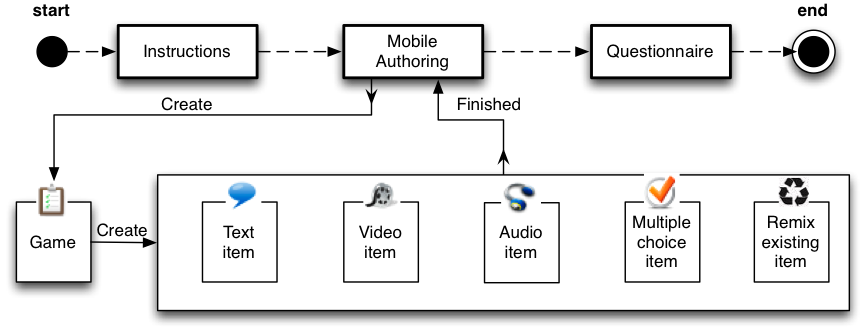
\includegraphics[width=0.9\linewidth]{img/mat_fig7}
	\caption{Flow of the experiment. UML-State diagram}
	\label{fig:mat_7} 
\end{figure}

\subsection{Instruments}
\label{sect:4_2}
The material for the study consisted in a first introduction of the experiment with a set of instructions to be read on paper, an Android smartphone (Sony XPeria S) with the \em MAT for ARLearn \em installed in it, and a desktop computer for accessing the post-questionnaire.

The System Usability Scale (SUS) was used for the evaluation of the usability \cite{Brooke1996}. The SUS scale consists of 10 questions with a five-point Likert scale, where item directions are changed in each question. The results of the survey were recorded in an online questionnaire. Based on the current literature, a SUS score above 68 (SD:12,5) is rated as usability score above average. This analysis have followed the recommendations from \cite{Sauro2011} so that the results can be mapped and benchmarked against 446 previous studies and 5000 individual responses.

\cite{Hassenzahl2001} has discussed the limitations of taking only into account usability and proposed in addition to take into account the ''hedonic quality'' of an interface. Hedonic quality is defined as the non-task related quality dimensions like ''accessibility'' or ''originality''. We employed the Reactiondeck toolkit developed by \cite{Benedek2002} to assess these aspects. These product reaction cards have been transferred to a digital version and published as Reactiondeck toolkit \citep{Storm2012}. Thus, participants were asked to select 6 product reaction cards that describe the emotional appeal of the mobile applications best and provide arguments on the selection (See Figure \ref{fig:mat_8}). After choosing the cards, users were invited to argue in an open text box why did they selected that card.
\begin{figure}
	\centering
     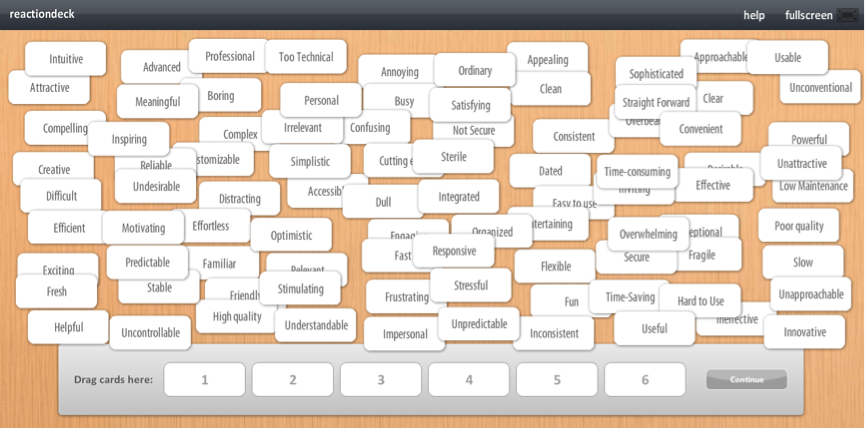
\includegraphics[width=0.9\linewidth]{img/mat_fig8}
	\caption{Evaluation of hedonic quality with the Reactiondeck \cite{Storm2012}.}
	\label{fig:mat_8} 
\end{figure}

\section{Results}
\label{sect:5}
Participants created (audio, text, video) resources to explain how to extend notebook�s screen to a bigger display, how to setup the fax, how to get cold sparkling water from the coffee machine, how to use the badge to access different buildings or how to play a demo in the eye-tracker of the lab (Figure \ref{fig:mat_5b}). Participants created multiple-choice questions to rate the quality of the printer, how clean is the lab, or the quality of the coffee machine. Participants remixed items like the photocopier instructions that only differed in the password depending on the building within the campus, or scanner instructions that differed in some steps depending on the brand of the device.

\subsection{Usability}
\label{sect:5_1}
The evaluation of the usability shows that \em MAT for ARLearn \em has a mean score of 80 (SD = 7.2), which is remarkably above average (SUS more than 68). Items 4 and 10 from the questionnaire were taken as subscale for learnability. Average learnability score was 17,81 where two participants (user 2 and 8) rated slightly below average. Items 1, 2, 3, 5, 6, 7, 8, 9 contribute to the construct usability where average score was 62,81 and only one participant rated below average (user 3).
\begin{figure}
	\centering
     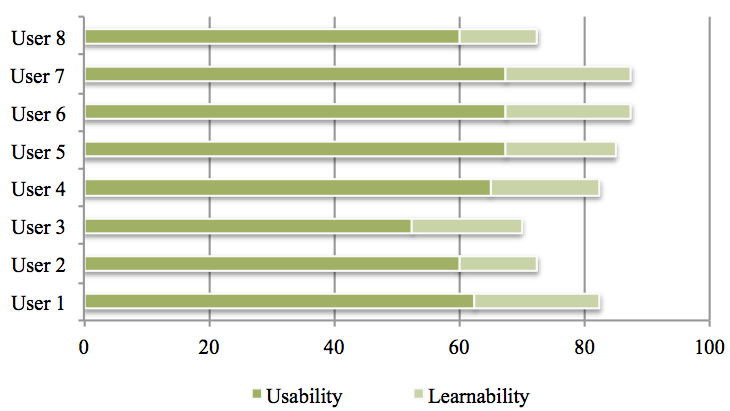
\includegraphics[width=0.9\linewidth]{img/mat_fig9}
	\caption{Evaluation of Usability and Learnability with the System Usability Scale (SUS) \cite{Brooke1996}.}
	\label{fig:mat_9} 
\end{figure}

\subsection{Hedonic quality}
\label{sect:5_2}
The Hedonic quality evaluation harvests adjectives that define the interface and usability of the tool considered in terms of pleasant (or unpleasant) sensations. Figure \ref{fig:mat_10} illustrates which were the most selected adjectives to determine the hedonic quality of the \em MAT for ARLearn\em . ''Organized'' and ''Usable'' were the most voted adjectives by the participants (n=4). E.g. regarding the organization users argued: ''\em The distribution of items, icons and buttons within the screen is consistent\em '', ''\em The interface is clear, and there are not useless elements on the screen. All of them are self-explanatory\em ''. These adjectives highlight a suitable distribution not only of the functionality across screens, but also of the elements (buttons, images, text boxes, etc.) used within the screens. Regarding the ''usability'' participants argued: ''\em The tool is intuitive and I feel confortable using it\em '', ''\em All choices for authoring are self-explained thus the tool is easy to use\em ''. Three participants selected ''Easy-to-use'' and two participants selected ''accessibility'' arguing ''\em It is easy to get access to configuration procedures of artefacts through mobile devices\em ''. These adjectives reveal an appropriate usability of the tool since participants could intuitively navigate without instruction and based on what they felt to be necessary. 

One participant highlighted the importance of providing open access to authored resources ''\em It is nice to share knowledge with others\em ''. This comment recognises the benefits of openly sharing knowledge as a way of actively promoting innovation, developing educational capacity and speeding up the processes by which researchers and academics review and build on each other�s work. On the other hand, the willingness of users to share their identify tagging authored educational resources with a suitable licence keeps being a controversy. In fact, two-participants reported their reluctance selecting the card for ''not-secure'' and arguing that ''\em The identity of the user might be in danger when sharing resources\em '', ''\em I am not happy sharing my identity when sharing content\em ''. 
\begin{figure}
	\centering
     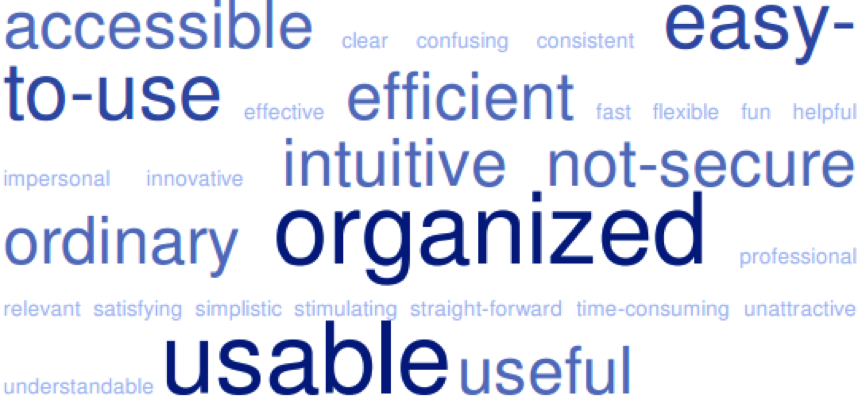
\includegraphics[width=0.9\linewidth]{img/mat_fig10}
	\caption{Tag cloud visualization for the measure of hedonic quality.}
	\label{fig:mat_10} 
\end{figure}

\section{Discussion and conclusions}
\label{sect:6}
The chapter has introduced the lack of authenticity in situated learning scenarios of desktop-based authoring systems in contrast to mobile-based authoring systems where resources can be enriched with users� context \citep{Specht2009}, \em namely \em , \em  location\em, \em time\em, \em environment\em, \em relation\em and \em artefact identification\em. This chapter proposes the use of mobile authoring tools not only as a solution to cover this gap, but also to foster universal access to educational resources. The review of scientific literature has revealed eight mobile tools for authoring of educational resources in a mobile context. These resources have been classified according to the Modular Content Hierarchy model \citep{Duval2003a}  (table \ref{tbl:map1}) with the aim to identify the grain of their authored resources towards the definition and the levels they can aggregate. Based on an analysis of these tools we have recognized ten shortcomings (L1 to L10) mobile authoring tools should cope to foster universal access to educational resources authored in a mobile context (see appendix C). 

These features have influenced the design and development of the \em MAT for ARLearn \em tool. In contrast to the existing standalone tools reviewed in this chapter, \em MAT for ARLearn \em has a scripting environment for mobile serious games for learning in the background. \em MAT for ARLearn \em has extended the state-of-art of authoring tools featuring 7 of the 10 limitations concluded in the literature review, namely,  (L1) share, (L2) remix, (L3) recontext, (L4) edit, (L5) search, (L6) licence support, (L9) use of sensors. This tool features searching, editing and sharing of learning OERs via Creative Commons licences facilitating the remix of contents. Moreover, \em MAT for ARLearn \em features the creation and contextualization of educational resources on two of the dimensions of the mobile context \citep{Specht2009}:
\begin{itemize}
\item Location. Users can bind authored resources to locations. E.g. an audio recording on a specific architecture linked to the geographical coordinates (longitude, latitude, radius) of a church (Figure \ref{fig:mat_4c}). Location coordinates can be obtained via GPS sensors in mobile phones.
\item Artefact identity. Users can bind authored resources to tags attached to physical objects. E.g. text instructions on how to use a photocopier linked to a QR code (Figure \ref{fig:mat_5c}). Barcodes or NFC tags are instances of artefact identifiers accessible via sensors in mobile devices.
\end{itemize}
Results of a usability evaluation have confirmed that the tool has usability above average and that users understand the functionalities of the tool. These findings are reinforced by the hedonic quality evaluation conducted. We believe that mobile authoring tools that allow for content sharing under open content licensed will be a key enabler for building an ecology of digital learning resources which are freely available in the direct environment of learners and which can be re-used, adapted and recontextualized. Moreover, both the measure of �usability� and �hedonic quality� presented in this chapter, can be taken as a reference for forthcoming developments of authoring tools serving as a base for future quantified and qualified comparisons. 

The review of authoring tools presented in this chapter is limited to systems found in scientific literature. This research should be extended to the ones existing in open app markets (Android, iOS, Windows, Blackberry, etc.). 
\em MAT for ARLearn \em is currently in BETA version and will be released in the Google Play market as one more feature within the framework (L8). 

In future research, we will develop and evaluate further features to (re)contextualize learning contents with the pending dimensions of the mobile context \citep{Specht2009}: time (e.g. a video recording on an specific historic which is only made available to appear on anniversary dates); relation (e.g. an educational resource that is only made available to appear when all the members of a group are together); environment (e.g. ''\em whenever the temperature is higher than 40 degrees, play an audio item on measures to prevent dehydration\em '').




		
\chapter{NFC LearnTracker: Binding personal learning goals to daily physical environments with mobile and sensor technology}



\vfill
This chapter presents the NFC LearnTracker, a mobile tool proposing the user to introspect his autobiography as a learner to identify successful physical learning environments, bind sensor tags to self-defined learning goals, keep track of the time invested on each goal with a natural interface, and monitor the learning analytics. This work implies a suitable tool for lifelong learners to bind scattered activities keeping them in a continuing learning flow. The NFC LearnTracker is released under open access licence with the aim to foster adaptation to further communities as well as to facilitate the extension to the increasing number of sensor and NFC tags existent in the market.
\vspace{3em}

This chapter is published as: 
Tabuenca, B., Kalz, M., \& Specht, M. (In Press). Binding daily physical environments to learning activities with mobile and sensor technology. In \em Communications in Computer and Information Science \em . 4th European Immersive Education Summit. Springer International Publishing, 

\clearpage

\section{Introduction}
Self-organized learning is one of the critical competences for individuals to cope with societal challenges and resulting changing demands on job markets. \cite{Eurostat2012} identified time, location and conflicts with other activities as the core barriers to lifelong learning. Nowadays, lifelong learners are confronted with a broad range of activities they have to manage everyday. In most cases they have to combine learning activities, professional and private life linking formal and non-formal learning activities. In the setting of an adult lifelong learner this is especially difficult as in most cases, interests might be highly distributed over different domains and keeping up learning needs an extra effort. One of the main challenges here is the bridging of learning activities between different contexts.

Mobile seamless learning technology can offer solutions to address this problem. Seamless learning was first defined as a learning style in which a learner can learn in a variety of scenarios and switching from one scenario or context to another using a personal device as a mediator \citep{Chan2006}. Succeeding, \cite{Wong2011d} identified ten gaps in seamless learning support: 1) Encompassing formal and informal learning; 2) Encompassing personalized and social learning; 3) Across time; 4) Across locations; 5) Ubiquitous knowledge access; 6) Encompassing physical and digital worlds; 7) Combined use of multiple device types; 8) Seamless switching between multiple learning tasks; 9) Knowledge synthesis; 10) Encompassing multiple pedagogical or learning activity models. Lately, a learner-centric view of mobile seamless learning \citep{Wong2012} suggests that \em a seamless learner should be able to explore, identify and seize boundless latent opportunities that his daily living spaces may offer to him (mediated by technology), rather than always being inhibited by externally-defined learning goals and resources \em. In the context of lifelong learners, three key problems need to be tackled:
\begin{itemize}
\item No support for learning activities across locations, devices, and environments. There is little research on how to link the different everyday contexts of lifelong learners and their learning activities in these different settings. (Seam 3, 4)
\item Linking learning activities with everyday life activities and the physical world objects. Everyday life events trigger different activities that lead to learning events. The linking between the self-directed learning of lifelong learners and their everyday environment is not foreseen in todays learning technology (Seam 1, 2, 7, 8)
\item Supporting reflection on learning activities and personal project in heterogeneous environments making use of different technologies (Seams 6, 9, 10).
\end{itemize}
In summary there is little support for lifelong learners that typically try to learn in different contexts, are busy with multiple parallel learning tracks, and must align or relate their learning activities to everyday leisure and working activities. \cite{Candy1991}  summarized four components of self-directed lifelong learning. These are \em self-monitoring, self-awareness, self-management \em (planning of learning) and\em meta-learning \em. To date, there is little technological support to enable learners in conducting these different activities across contexts and locations. A recent survey to lifelong learners on mobile usage habits reveals that there is an association between the type of learning activity being performed (read, write, listen, watch) and the specific space where it normally takes place \citep{Tabuenca2013}. Hence, there is a need to provide suitable tools for lifelong learners to facilitate bridging learning experiences in a seamless flow. In this chapter Near Field Communication (NFC) is proposed as an instantiation for natural interaction with mobile devices and for seamless integration of technology in lifelong learning.

The following section reviews previous research of scientific work where NFC has been used with learning purposes. Section 2 identifies the four pillars sustaining the design of a mobile tool for self-regulated support: NFC LearnTracker. In section 3 the core features are described and the results of a prototype formative evaluation are presented. 
\subsection{Using NFC tags for bridging seams and natural interaction}
\em Natural User Interfaces \em and the \em Internet of Things \em have been predicted to have an impact on education in the short term \citep{Johnson2012}]. Tagged objects are widely accepted and the number of connected devices could reach 50 billion by 2020 \citep{Ericsson2011}. Different tagging methods (e.g. visual codes, text recognition, image recognition) allow enriching physical objects of the world with educational resources. Moreover, the prominent adoption of NFC readers in mobile devices has moved this technology from an innovator to an early adopter phase. This frictionless technology will enrich our environment facilitating natural interactions with daily physical objects. NFC simplifies and reduces several actions to a single action of narrow contact (zero click overhead). These small exchanges of information between devices that occur almost instantaneously have been coined as \em micro-interactions \em \citep{Dodson2012}.

Recent work reviews scientific literature in which NFC technology has been used with learning purposes \citep{Tabuenca2014b}. More specifically, \cite{Ebner2013} present some of the potentials NFC technology brings for teaching and learning materials in formal education: distributing learning/teaching materials in face-to-face classrooms; enriching printed materials; sharing materials among students; delivery of practical work; bind physical actions to social networks; access to control materials; identification of students in examinations. Likewise, there is an increasing number of empirical studies using NFC technology in field trips \citep{Kuflik2011,Perez-Sanagustin2012}, connecting digital and physical worlds \citep{Kubicki2011,Ailisto2006,Munoz-Organerooo2010} or combining this technology within Learning Management Systems \citep{RamirezGonzalez2012}. Nevertheless, NFC has not been used to tackle the problems of lifelong learners. In the following we will frame and integrate these approaches according to the model of \cite{Candy1991} introduced in the introduction of this chapter.

The work from \cite{Ebner2013} highlights the incompatibility between existing NFC-tags and NFC-readers as one of the main barriers blocking further expansion of the NFC technology. For example, chips produced by one specific manufacturer perfectly work with their own tags but, other tags are not readable by chips produced by other manufacturers although their data format is based on the standard. It is one of the goals of this research to implement a generic open source architecture to facilitate its extension across NFC readers and tags.
\section{Design of the NFC LearnTracker}
The NFC LearnTracker is a standalone application developed for NFC-enabled Android (4.03 or above) devices released in March 2014 in Google Play\footnote{NFC LearnTracker in Google Play. https://play.google.com/store/apps/details?id=org.ounl.lifelonglearninghub}. The NFC LearnTracker uses an embedded database for local storage in the same application software to avoid privacy issues of sharing data. The NFC LearnTracker is part of a larger research (Lifelong Learning Hub Project) aiming to provide ubiquitous support for lifelong learners. It has been released trusting open source code license, made available in a repository\footnote{Lifelong Learning Hub�s code repository. https://code.google.com/p/lifelong-learning-hub/} to be downloaded, customized and further extended to different learning environments, LMSs, or communities. This section presents the NFC LearnTracker as mobile seamless tool for self-regulated learning that aims to cover the following gaps in lifelong learners� learning process:
\begin{enumerate}
\item No support for learning activities across locations, devices and environments.
\item No linking between learning activities and everyday life.
\item No feedback on lifelong learning activities.
\item Incompatibility between NFC-tags and NFC-readers.
\end{enumerate}
\subsection{Self-regulation across contexts with mobile learning analytics}
The NFC LearnTracker has been designed based on the seamless notion that lifelong learners can learn in a variety of scenarios switching from one scenario or context to another easily and quickly, using the personal device as a mediator. Figure \ref{fig:nfclt_1} illustrates how daily life activities and learning activities are combined in a continuing process. The tool presented in this section has been conceptualized on the idea that mobile technology can be smoothly integrated in daily life activities whenever interacting with it requires the least number of clicks possible (zero) and the duration of any interaction with the tool lasts not longer than 20 seconds. 

\cite{Butler1995} describe the Self-Regulated Learning Model as an iterative process comprising four sequential stages: 1) interpretation of own learning paths and task queuing; 2) cognitive process of defining goals and monitoring the progress; 3) perform the learning activity; 4) interpretation of external feedback. Similar and focusing on lifelong learners, \cite{Candy1991} proposes a learner-centric model with four stages (See section 1). Hereby we describe in a narrative scenario \citep{Carroll1999} how these stages have been covered with the NFC LearnTracker bringing a character to life: Miguel Angel, a PhD student aiming to combine his daily life activity (family, work, leisure) with learning activities towards the accomplishment of his doctoral degree.
\begin{figure}
     \centering
     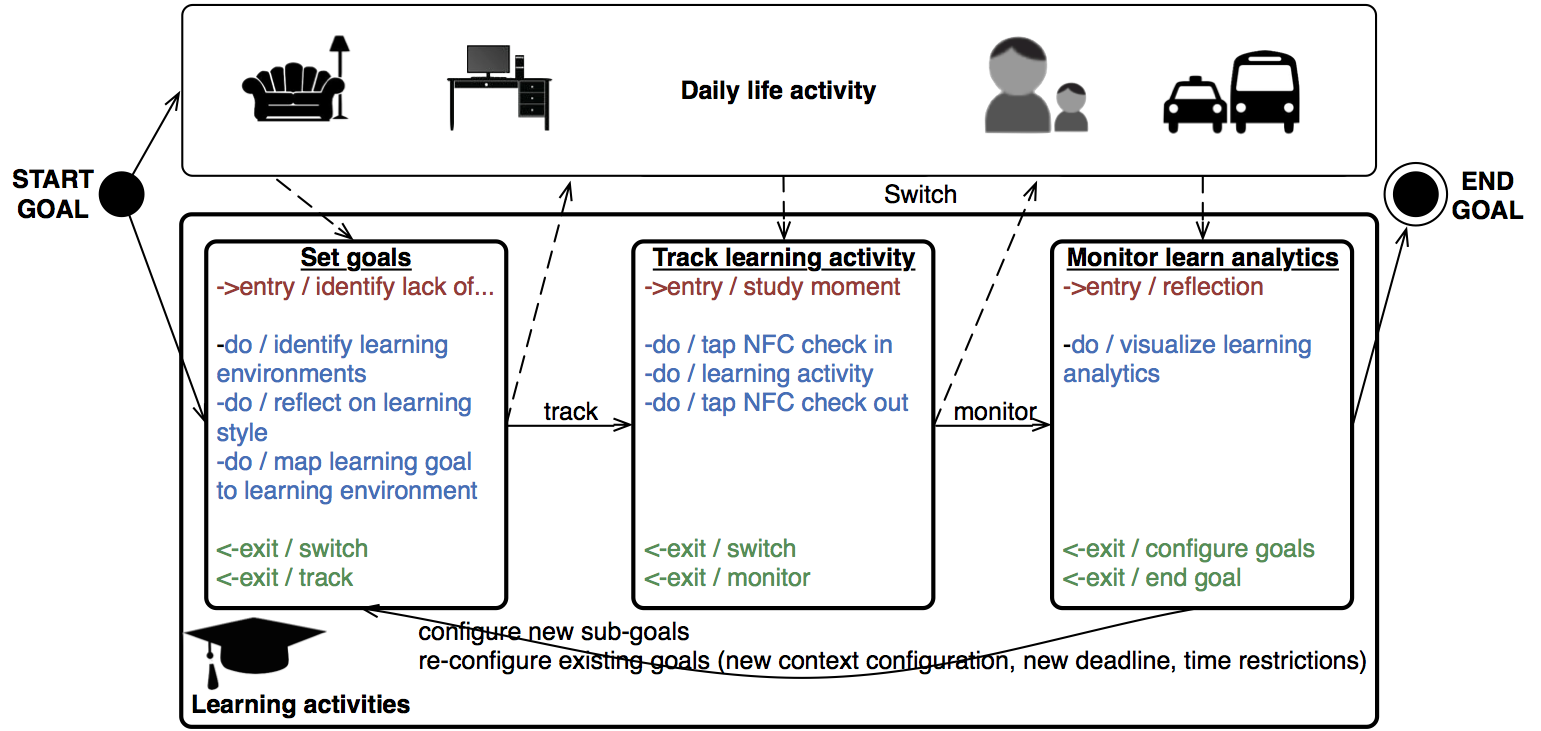
\includegraphics[width=1\linewidth]{img/nfclt_fig1}
     \caption{Lifelong learner's goal life cycle. UML state diagram}
     \label{fig:nfclt_1}
\end{figure}
\subsubsection{Set learning goals}
Miguel wants to improve on academic writing, developing his skills to make effective presentations in public, broadening English vocabulary, and setting aside time to read scientific literature. As he engages in these learning tasks, he draws on knowledge and beliefs constructing an interpretation of each task�s properties and requirements \citep{Butler1995}. In fact, Miguel frequently introspects his autobiography as a learner to identify which learning environment fits better to which learning task upon his learning style or time availability. This stage covers the � \em Planning for learning \em � and � \em self awareness \em � stages in the self-regulation model for lifelong learners \citep{Candy1991}. Analogously, \cite{Butler1995} situate the stage of � \em setting goals \em � within the cognitive system stressing its key importance in shaping the process of self-regulated learning.  

In this stage (first box in figure \ref{fig:nfclt_1}), Miguel reflects on his learning style mapping learning goals to frequently used learning environments and tagging them with NFC tags (See figure \ref{fig:nfclt_3}). Whenever Miguel configures his goals in the NFC LearnTracker, he takes a NFC tag, taps it with his NFC enabled mobile device so the interface in figure \ref{fig:nfclt_2a} is displayed. He characterizes the goal with a name e.g. \em Academic Writing \em, specifies the expected outcome e.g. \em Publish on a highly ranked SSCI journal \em  when he accomplishes the goal, foresees how much time (in minutes) will he devote to this goal on daily basis e.g. \em 60 mins \em , and finally indicates his expected date to finish the goal e.g. \em 3rd June 2015 \em . Sticking a NFC tag on a physical learning object enables the connection of a variety of tracking data with the learning activity as Miguel can identify how much time does he use a specific device for reading (e.g. tablet, book, laptop), the location where he devotes more time to learn or the least productive days of the week. The learning goals dashboard (figure \ref{fig:nfclt_2b}) lists all the goals configured by the user.
\begin{center}
\begin{figure}[ht]
\centering
	\subfloat[Linking a purple NFC tag to Academic Writing learning goal]{
		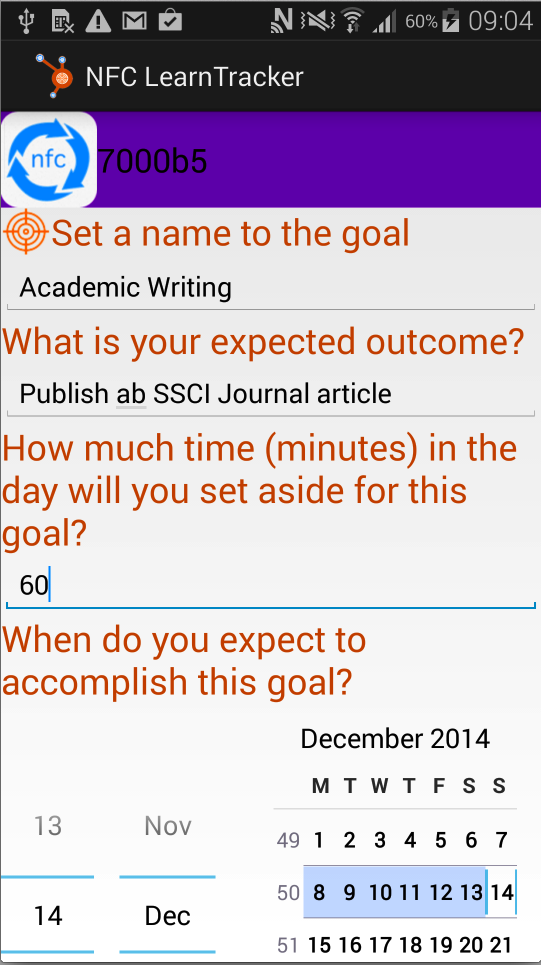
\includegraphics[width=0.3\linewidth]{img/nfclt_fig2a}
		\label{fig:nfclt_2a}
	}
	\subfloat[Learning goals configured by the user]{
		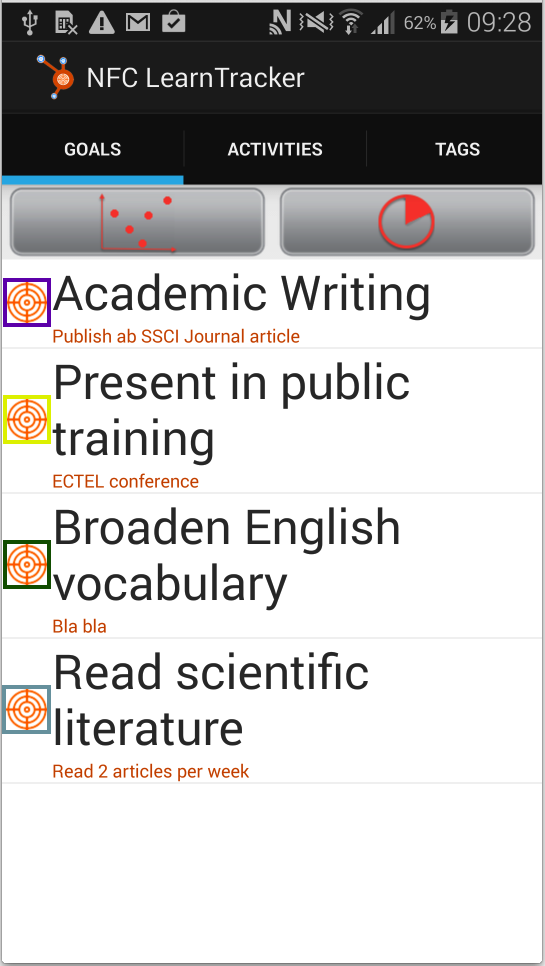
\includegraphics[width=0.3\linewidth]{img/nfclt_fig2b}
		\label{fig:nfclt_2b}
	}	
	\subfloat[�Check-in� registered for Academic Writing and event history]{
		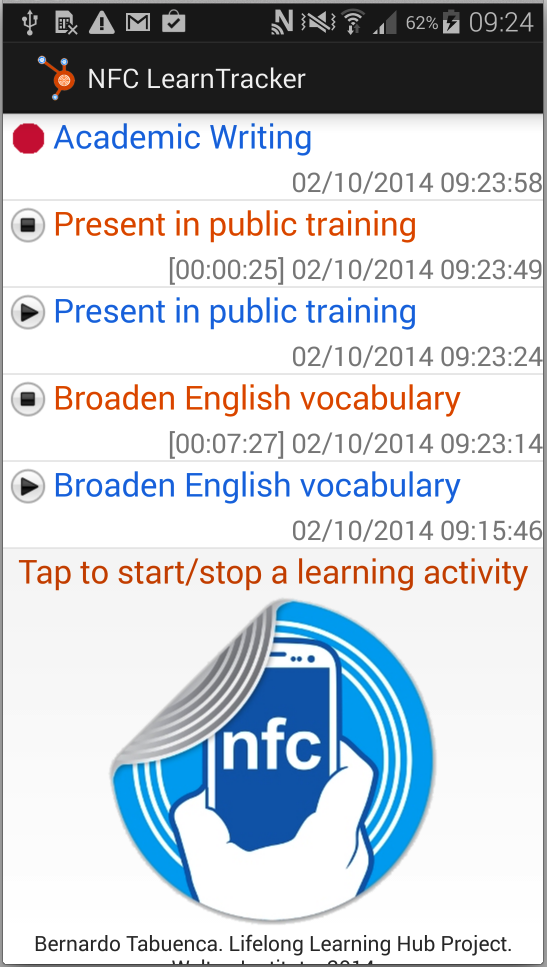
\includegraphics[width=0.3\linewidth]{img/nfclt_fig2c}
		\label{fig:nfclt_2c}
	}	
      \caption{Binding goals to tagged learning environments via NFC-LearnTracker}
      \label{fig:nfclt_2}
\end{figure}
\end{center}
\subsubsection{Perform learning activities}
Miguel, as most of the lifelong learners, recurs to specific locations (e.g. desktop, coach) and moments (e.g. waiting times, transitions) to accomplish his learning activities \citep{Tabuenca2013}. In addition, Miguel is interested to know how much time he devotes to learning during the day and along the week so he can also reserve time to enjoy the family. Hence, Miguel needs a tool with natural interaction, otherwise he will not bother to track short learning moments (e.g. fifteen minutes writing, figure \ref{fig:nfclt_3a}; twenty minutes reading, figure \ref{fig:nfclt_3b}; ten minutes listening podcasts, figure \ref{fig:nfclt_3c}; three minutes watching videos, figure \ref{fig:nfclt_3d}), and as result these moments will never be accounted as learning time. The NFC LearnTracker harvests all learning moments accounting them as real learning time with frictionless interactions. Both self-regulation models cited above \citep{Candy1991,Butler1995} situate this stage out of the scope of the cognitive system.

In this stage (second box in figure \ref{fig:nfclt_1}) Miguel taps the associated NFC-tag every time he wants to start \em check-in \em / stop \em check-out \em a learning activity. Figure \ref{fig:nfclt_2c} illustrates with a red dot the moment in which time devoted to the goal � \em Academic Writing \em � is being recorded as an effect of tapping the tag once. The history of the subsequent events is registered as a log.
\begin{center}
\begin{figure}[ht]
\centering
	\subfloat[Write an article taking the first coffee in the morning at work]{
		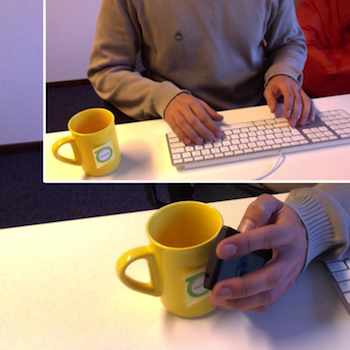
\includegraphics[width=0.22\linewidth]{img/nfclt_fig3a}
		\label{fig:nfclt_3a}
	}
	\subfloat[Reading scientific literature during waiting times]{
		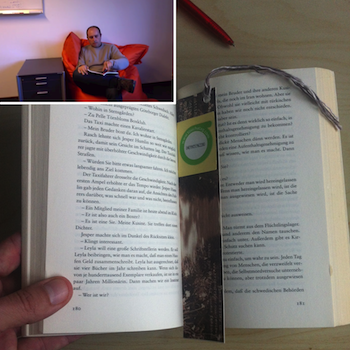
\includegraphics[width=0.22\linewidth]{img/nfclt_fig3b}
		\label{fig:nfclt_3b}
	}	
	\subfloat[Listening English podcasts commuting to work, college, gym...]{
		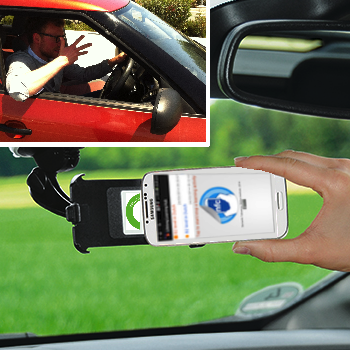
\includegraphics[width=0.22\linewidth]{img/nfclt_fig3c}
		\label{fig:nfclt_3c}
	}	
	\subfloat[Watch top presenters� videos during commercial breaks]{
		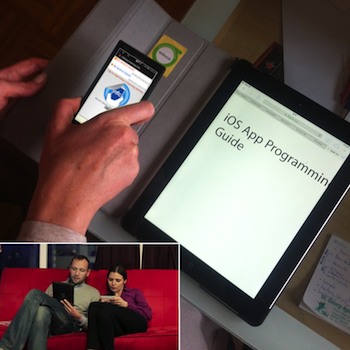
\includegraphics[width=0.22\linewidth]{img/nfclt_fig3d}
		\label{fig:nfclt_3d}
	}		
      \caption{Learning activities (write, read, listen, watch) bound to daily learning environments}
      \label{fig:nfclt_3}
\end{figure}
\end{center}
\subsubsection{Monitor learning activities}
The NFC LearnTracker features learning analytics when defined as �\em the measurement, collection, analysis and reporting of data about learners and their contexts, for purposes of understanding and optimising learning and the environments in which it occurs \em �\footnote{1st International Conference on Learning Analytics and Knowledge. International Conference on Learning Analytics and Knowledge. p. 2011, Alberta (2011)}. Monitoring the state in learning activity can motivate the user towards the accomplishment of a learning goal. By comparing evolving states of a task to goals creates conditional knowledge that is the basis for further action. This cognitive process has been defined as � \em internal feedback \em � \citep{Butler1995}, � \em self monitoring \em �, and � \em understanding how to learn \em � \citep{Candy1991} in the previously cited self-regulation models. The cues identified by the user in this process facilitate the recognition of his learning patterns and as a result, the constant update of his autobiography as a learner.
\begin{center}
\begin{figure}[ht]
\centering
	\subfloat[Quantity of time invested in learning goals (Percentage or overall time and number of minutes)]{
		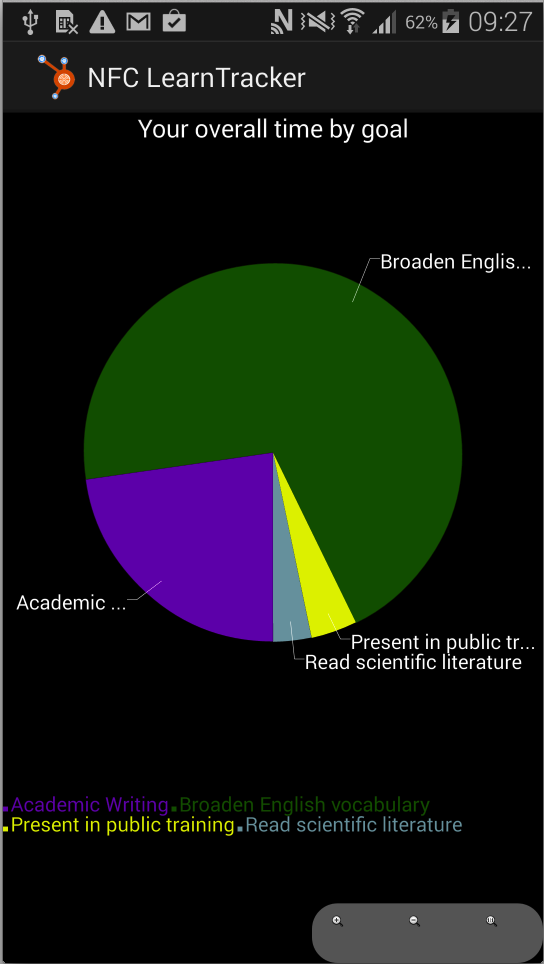
\includegraphics[width=0.3\linewidth]{img/nfclt_fig4a}
		\label{fig:nfclt_4a}
	}
	\subfloat[Distribution of learning moments along the day in the last 7 days]{
		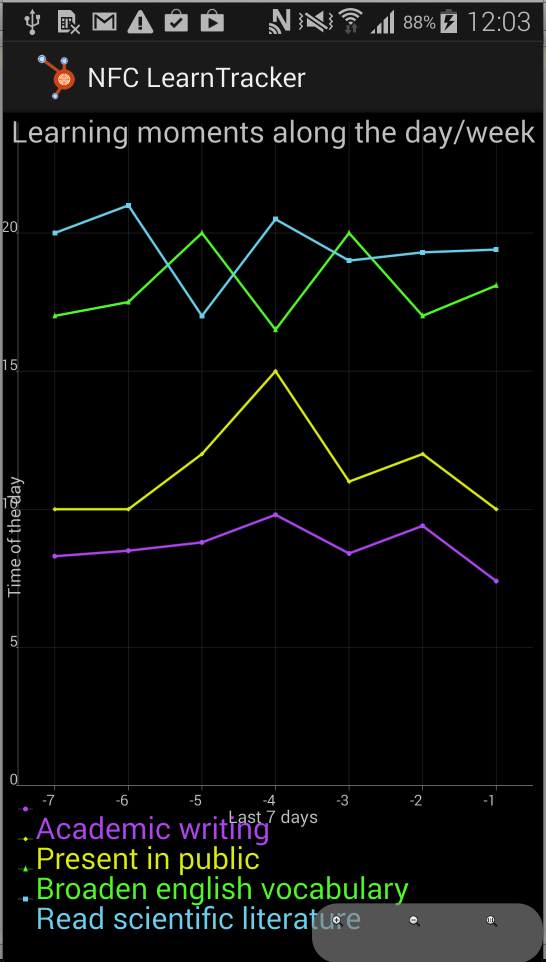
\includegraphics[width=0.3\linewidth]{img/nfclt_fig4b}
		\label{fig:nfclt_4b}
	}	
	\subfloat[Foreseen learning time (orange) versus effective time invested (in purple) on Academic Writing in the week]{
		\includegraphics[width=0.3\linewidth]{img/nfclt_fig4c}
		\label{fig:nfclt_4c}
	}	
      \caption{Learning analytics in NFC LearnTracker}
      \label{fig:nfclt_4}
\end{figure}
\end{center}

In this stage (see third box in figure \ref{fig:nfclt_1}), Miguel can monitor his learning analytics on a specific goal, or as overall performance. \cite{Siemens2011} stressed that the focus of learning analytics is exclusively on the learning process. Hence, the NFC LearnTracker tracks and visualizes data about the learning process within the specific personal learning context for which they were configured by the lifelong learner, and independently from the content (subject, topic, etc.) that is learned in the process. The NFC LearnTracker features a charting library\footnote{AChartEngine Library: https://code.google.com/p/achartengine/} that facilitates the implementation of several visualizations. As of date December 2014, the NFC LearnTracker provides the following visualizations with the aim to foster understanding on learning habits, optimise learning, and, bind successful learning environments:
\begin{enumerate}
\item\em Percentage of time invested on each learning goal \em (fig. \ref{fig:nfclt_4a}). Learning activities are scattered along the day in different locations or transitions. This feature provides lifelong learners an overall summary on how much time is devoted to learning goals. Figure \ref{fig:nfclt_4a} illustrates how percentage of total time and number of minutes are presented in a pie chart. This visualization can be used by lifelong learners to compare time invested on his learning goals, identify priorities to accomplish goals, and, patterns regarding preferences for specific learning environments, devices or learning activities (read, watch, write, listen).
\item\em Distribution of learning moments along the day \em  (fig. \ref{fig:nfclt_4b}). Every lifelong learners performs differently in the sense that some of us prefer to do learning activities that require a higher cognitive load or concentration in early morning (scientific reading or writing), or do the ones that require least cognitive load while sat on the couch at night during every commercial pause on TV (watch videos or dispatch emails). Lifelong learners are intrinsically interested to identify patterns in their learning experiences and scaffold their autobiography as a learner to better distribute learning activities in forthcoming goals. Figure \ref{fig:nfclt_4b} illustrates the distribution of the learning moments during the day (X axis 0..24) for a whole week (Y axis 1..7). Each spot (square, triangle, circle) identifies when the learning activity started. 
\item\em Monitoring accomplished goals \em (fig. \ref{fig:nfclt_4c}). Monitoring is of crucial importance in relation to the development as a self-regulated learner. Monitoring is the cognitive process that assesses states of progress to goals and generates feedback that can guide further action \cite{Butler1995}. Figure \ref{fig:nfclt_4c} illustrates a representation of accomplished learning time versus expected time towards a learning goal NFC LearnTracker.
\end{enumerate}
\subsection{An open source NFC implementation}
There is a huge number of NFC tags available in the market. An NFC tag is a small passive (no battery) device that contains a microchip attached to a small loop antenna. When an NFC reader such as a mobile phone scans the tag, it powers up and wirelessly transfers information such as a web address, text or a command for an app. NFC tags are typically printed stickers, but they can be also enclosed in NFC products such as wristbands, hang tags and other artefacts. 

There is no way to create an app capable to interpret the information encoded in every NFC tag available on the market. Nevertheless, it is possible to provide suitable guidance on how to extend the software to be compatible with further tags and readers. All NFC enabled phones currently on the market can read a web address (URI) or text. The NFC LearnTracker features NFC standards\footnote{NXP: NFC Forum Type Tags White Paper. (2009)} (Figure \ref{fig:nfclt_5}) implementing the following interfaces:
\begin{itemize}
\item \em UriRecord \em tag is used to launch an URL in the mobile�s browser
\item \em TexRecord \em tag is used to complete a text field within an app in the mobile
\item  \em SmartPosters \em tags is used in public static commercials to launch multimedia on user�s device
\end{itemize}
Moreover, the LearnTracker has been developed following an architecture that facilitates its extension to more complex NFC tasks like command execution, and to enable the compatibility across NFC-tags and NFC-readers. When extending the use of tool to a new tag standart type, a new class must be created implementing the interface \em IParseNdefRecord \em so the methods \em getId() \em to indicate a unique identifier for the tag (e.g. http://www.ou.nl/293903843),\em getType() \em to indicate the name of the standard type (e.g. UriRecord), and \em getColor() \em to indicate the colour in RGB hex that will be used in the charts to identify the mapped goal (e.g. "ACDCED" for a light blue tag).
\begin{figure}
     \centering
     \includegraphics[width=0.9\linewidth]{img/nfclt_fig5}
     \caption{Tag extension in NFC LearnTracker}
     \label{fig:nfclt_5}
\end{figure}
\section{Formative evaluation}
This tool was presented to 14 PhD students attending to a workshop in March 2014. The concept of lifelong learning and the scope of the research were introduced and the problems described in the introduction section of the current chapter were enumerated. With this focus in mind, the tool was presented for 30 minutes as a potential solution to those problems providing practical examples, making a demo with physical learning environments where the tool can be used, and highlighting the natural interaction of the NFC micro-interactions. After that, participants completed a questionnaire containing eight 5-likert-scale questions prompting the participants to reflect and rate the potential of the tool to: manage learning goals; foster awareness on preferred learning environments; integrate learning with daily life activities; learning activities across contexts; set aside time to learn on regular basis; adjust goals; set mini-goals along the way; overall rating of the mobile tool to define goals, set-aside time, bind goals to daily activities, keep track of time invested on each goal, and monitor these analytics.

In the last part of the session, an open discussion was proposed around the following two questions: (1) �\em What kind of feedback do you find suitable to be provided with this tool? \em �. Tips for productive listening, writing or reading were highlighted as a potential feedback supplied in the form of pushed notifications. E.g. Participant\#4 suggested that it might be interesting if she would receive a notification prompting to identify her learning goals before starting the lecture, or suggesting tips for productive listening like (e.g. taking notes or asserting). Participant\#7 stressed that notifications prompting to reflect on what has been learned after accomplishing the learning activity could help to make knowledge more persistent. Participant\#8 suggested that it would be interesting to rate my perceived productivity after a learning activity and correlate it with the time of the day, day of the week, duration of the task, type of device used or location where I accomplished the learning activity. Participant\#3 suggested providing a notification when to consider making a break every 2 hours.

A second question 2 proposed a discussion about (2) �\em In which learning scenarios do you consider this tool can be applied? \em �. Participant\#1 suggested extending the scope of the mobile tool from self-regulation to a scenario in formal education. �\em Books in secondary school could be NFC-tagged so that the teachers could use this tool to get a grasp on which subjects do students invest more/less time in their homework \em �. Participant\#9 stressed the importance of the tool for self-awareness �\em this tool could help me to establish some limits to the time I invest in non-academic tasks versus the time I invest in academic tasks \em �. Participant\#3 stated, �\em Sometimes you are so tied up with concrete projects that you really need to stop, reflect and organize your learning goals. This tool can be not only used to organize your learning time but also any other daily life activity \em �. Upon all these statements, several participants pinpointed to the learning analytics illustrated in figure \ref{fig:nfclt_4} as a very interesting feature to quantify your learning style and become aware of the time devoted to learning activities in long term.
\begin{table}[h]
  \centering
  \footnotesize
  \caption{Evaluation of the NFC-LearnTracker. 5-likert scale (5:�strongly agree�, 1:�strongly disagree�)}
  \label{tbl:nfclt_table1}
\begin{tabular}{lllll}
\thickhline
\textbf{Potentials of the tool} 											& \multicolumn{1}{c}{\textbf{SD}}						& \multicolumn{1}{r}{\textbf{AVG}}              & \textbf{} & \textbf{} \\ \thickhline
Manage learning goals                             							& \multicolumn{1}{r}{0.84}                            	& \multicolumn{1}{r}{3.36}                       &           &           \\ 
Foster awareness on preferred learning environments     					& \multicolumn{1}{r}{0.70}                           & \multicolumn{1}{r}{3.79}                       &           &           \\ 
Integrate learning with daily life activities           					& \multicolumn{1}{r}{0.61}                             & \multicolumn{1}{r}{3.29}                       &           &           \\ 
Learn across contexts                             							& \multicolumn{1}{r}{0.78}                             & \multicolumn{1}{r}{3}                       &           &           \\ 
Set aside time to learn on regular basis                             		& \multicolumn{1}{r}{1}                             & \multicolumn{1}{r}{3.07}                       &           &           \\ 
Adjust goals high enough to challenge but not so high to frustrate you      & \multicolumn{1}{r}{1.12}                             & \multicolumn{1}{r}{3.21}                       &           &           \\ 
Set mini-goal along the way                             					& \multicolumn{1}{r}{0.73}                             & \multicolumn{1}{r}{3.93}                       &           &           \\ 
Overall rating                             									& \multicolumn{1}{r}{0.75}                             & \multicolumn{1}{r}{3.43}                       &           &           \\ \thickhline
\end{tabular}
\end{table}
\section{Conclusions and future work}
The observations on the lifelong learning process indicate that typical learning activities of continuing and further education are poorly connected to the daily activities of the learners. There is no support for learning activities across locations, devices and environments and there is a need to provide customized feedback to lifelong learning activities. The tool presented in this chapter represents an approach to these problems. Tracking when, where and how learning occurs along the day provides rich information to infer lifelong learner�s owns habits. This paper reviews previous work on educational scenarios using NFC and four pillars for seamless support of lifelong learners are identified. The NFC LearnTracker has been presented and evaluated as a tool to lead lifelong learners towards a self-regulated process: fostering awareness on learning goals and learning moments; facilitating the user to keep track of learning time with a natural interface; fostering engagement and motivation on the task providing feedback with useful statistics. The Lifelong Learning Hub Project\footnote{Lifelong Learning Hub Project site. https://sites.google.com/site/lifelonglearninghubproject/} has been released under open licences with the aim to foster its adaptation to further educational communities as well as to facilitate the extension to the increasing number of NFC tags existent in the market.

As limitations, the evaluation of this tool has been performed in an artificial context (Technology Enhanced Learning workshop). The NFC LearnTracker should be tested in longitudinal studies with personal mobile devices and in lifelong learning settings. A realistic scenario must contemplate that the single decision to start using the tool should be triggered by an intrinsic motivation from the user to explore his learning patterns rather than an externally proposed task. The effects in self-regulation and intrusiveness of logging learning time and monitoring learning patterns should be explored in further research. This tool might be an interesting approach to determine whether students with more scattered and shorter learning moments are correlated with better or worst performance.

In further research, we will investigate the effects in self-regulation of self-defined internal feedback loops \citep{Narciss2007} via ambient learning displays \citep{Borner2013} based on the patterns identified with the NFC LearnTracker. This feedback will be mapped to the check-in and check-out events so users can customize and receive stop-and-think signals to reflect when starting a learning activity, doing it or finishing it \citep{Tabuenca2014}. 

The contribution of this chapter is presenting a tool for lifelong learners to bridge scattered personal learning environments in which learners can define personal ecologies and experience the interaction with such a system in long term typical lifelong learner settings. This research aims at giving an open, flexible and low-cost prototyping framework for defining and linking everyday learning activities to contexts, physical artefacts, everyday home media solutions, and supporting to link sustainable learner tracks to these components.		
		% To-Dos:

\chapter{Would you please warn me?: Self-configuration of feedback at workplace towards validity of time management . IN PROGRESS} % Write in your own chapter title

%\begin{quote}
%\textbf{Abstract:} With a focus on the situated support of informal and non-formal
%learning scenarios in ubiquitous learning environments, the presented paper outlines the authors� vision of ambient learning displays � enabling
%learners to view, access, and interact with contextualised digital content
%presented in an ambient way. The vision is based on a detailed exploration of
%the characteristics of ubiquitous learning and a deduction of informational,
%interactional, and instructional aspects to focus on. Towards the vision essential
%research questions and objectives as well as a conceptual framework that
%acquires, channels, and delivers the information framed in the learning process
%are presented. To deliver scientific insights into the authentic learning support
%in informal and non-formal learning situations and to provide suggestions for
%the future design of ambient systems for learning the presented paper concludes with a
%research agenda proposing a research project including a discussion of related
%issues and challenges.
%\end{quote}
\vfill
Nowadays, smartphone users bla bla
\vspace{3em}

This chapter is published as: 
Tabuenca, B., Kalz, M., \& Specht, M. (2015). (Submitted) Time will tell: Self-regulation of time with mobile learning analytics. \em IEEE Transactions on Learning Technologies (TLT) \em, (Special Issue on Seamless, Ubiquitous, and Contextual Learning), 1�12. doi:10.1109/TLT.2014.2383611

\clearpage

\section{Introduction}


\section{Study}
\subsection{Method}
\subsubsection{Participants}


\subsubsection{Materials}

\subsubsection{Design}

\subsubsection{Procedure}
\subsection{Results}
   
\section{Discussion and conclusions}
		
		%\clearpage{\pagestyle{empty}\cleardoublepage}	
		\addtocontents{toc}{\protect\newpage}
	
	\part{Empirical findings}
		\chapter{Stop and think: Exploring mobile notifications to foster reflective practice on meta-Learning} 

\vfill
This chapter explores the effectiveness of mobile notifications to foster reflection on meta-learning by presenting the results of two studies: 1) a formative study with 37 secondary school students offering a daily reflection and reporting exercise about their learning experience during the day; 2) an experiment involving 60 adults to read an eBook on energy-efficient driving for one hour. During that time, the participants received mobile notifications inviting them to reflect in-action. On the one hand, the results from the first study show that students do not have a habit of seeing themselves as learners and developing a \em ''professional'' \em awareness about their daily activity at work/school. On the other hand, the second study explores the effects of different notification types on knowledge gain and motivation. Results envision a higher knowledge gain and motivation for the group assigned with the least complex interactions with mobile devices during the reflection exercise.
\vspace{3em}

This chapter is published as: 
Tabuenca, B., Kalz, M., Ternier, S., \& Specht, M. (2014). Stop and think: Exploring mobile notifications to foster reflective practice on meta-learning. \em IEEE Transactions on Learning Technologies\em . Special Issue on Seamless, Ubiquitous, and Contextual Learning. 1�12. doi:10.1109/TLT.2014.2383611

\clearpage

\section{Introduction}

Based on current trends \citep{Publishing2011}, it is estimated that 84 percent of today�s young people in OECD countries will complete upper secondary education over their lifetimes. This period consolidates students� basic skills and knowledge towards a successful transition to either an academic or a vocational pathway. While graduation rates give an indication of the extent to which education systems are succeeding in preparing students to meet the labour market�s minimum requirements, they do not capture how the students have developed an identity as learners. The acquisition of such an identity, and the associated reflective transversal skills, grow in importance in a \em ''lifelong learning society'' \em  \citep{EuropeanComission2005}. In the formal education system it is a challenge to find ways to provide students with opportunities to mentally evoke what they have learned throughout the day, so that this experience can be turned into a deliberate object of attention and reflection.

\em Learning to learn  \em and \em Digital competence  \em are highlighted as two of the eight key competences for lifelong learning in the European Reference Framework \cite{EuropeanCommission2007}. The proliferation of wirelessly-networked technologies facilitates the scaffolding of \em seamless learning spaces \em \citep{Chan2006} as an approach for continuing learning experiences across different scenarios, and emerging from the availability of one device or more per person. \cite{Biggs1985} defines meta-learning as an awareness and understanding of the phenomenon of learning itself as opposed to subject knowledge. Hereby we conceive meta-learning activities as the increase of knowledge and motivation on learning when triggered by introspective episodes of reflection on user�s own learning. Hence the present chapter explores different instantiations of notifications received on mobile devices with the aim to foster reflective practice for meta-learning measuring the variations in dependent variables of knowledge and intrinsic motivation.

Reflection is the practice to become aware of an implicit knowledge base and to learn from experience \citep{Schon1983}. Sch\"on coined the terms \em reflection in-action \em as the reflective practice performed while doing an activity to optimize the immediately following action, and, \em reflection on-action \em as the reflective practice performed when the activity has finished in order to review, analyse, and evaluate the situation and gain insight for improved practice in the future.

Previous work on reflection amplifiers in-action suggests that regular changes between meta-cognitive and content focus lead to more awareness and self-regulative competences in the learning process \citep{Bannert2009,Verpoorten2012}. Reflection amplifiers are compact and well-considered prompting approaches that offer learners structured opportunities to examine and evaluate their own learning \citep{Verpoorten2009}. They are present as structured and repeated introspective episodes, offered in the course of action and meant to make learning visible. The effectiveness of mobile notifications to foster reflective practice on learning (reflection on-action) has not been explored yet. Recent research suggests that mobile notifications by students produce distracting effects \citep{Fried2008,Kraushaar2010}. Nonetheless, notifications received on mobile devices have also resulted in a positive impact, suggesting that the intervention is able to improve students� self-regulated learning effort. The study from \cite{Goh2012a} used persuasive SMS interventions on undergraduate students for 12 weeks, showing that students who received SMS intervention performed better than students who did not receive SMS intervention. \cite{Cavus2009} investigated the effects in knowledge and enjoyment of sending SMSs with English vocabulary to 45 first-year undergraduate students concluding that students enjoyed and learned new words with the help of their mobile phones. Similar, \cite{Thornton2005} used more elaborated notifications in the form of emails to teach English vocabulary lessons to university students concluding that students that received the mobile email learned more than those that received web-based email. \cite{Uzunboylu2009} implemented multimedia messages to increase awareness on environmental concerns. Measures of enjoyment, knowledge or awareness have been the focus of previous research.

This chapter presents two studies evaluating approaches to stimulate learners� capacity of reflection by making \em what they learn \em  a deliberate object of attention \citep{Watkins2001}. The research is embedded into a larger project focusing on mobile support for lifelong learning \citep{Tabuenca2013,TabuencaCAA2014,Tabuenca2014d}. More specifically, in this work we have focused on the use of notifications instantiated in mobile devices for lifelong learning support. Research on notification and prompting for reflection suggest different strategies for reflection on-action and in-action. This work advances the research on mobile notifications and reflective practice presenting two studies:
\begin{itemize}
\item A formative study aimed to reflect on-action. This study was carried out during two school days and two days off, where 37 college pupils were prompted via mobile SMS notification for a daily reflection and reporting exercise about how they have learned during the day (intensity and channels).
\item An experimental study aimed to reflect in-action. In this study, 60 university employees were invited to read an eBook on energy-efficient driving. During that time, they were prompted via mobile notifications to reflect and report on what they had learned.
\end{itemize}
The following sections introduce both experiments by mapping the goal of the research to existing gaps that need to be covered. The results are discussed and important research questions are raised.

\subsection{How to design mobile notifications for student reflection support}
The first study presented in this chapter transposes \em reflection amplifiers \em \citep{Verpoorten2009} to mobile (meta-)learning, after-school setting and analytical scrutiny onto one�s learning day.  In this study, students have been assigned to reflect about the learning affordances offered to them throughout the day. Three main research questions have guided this formative study:
\begin{enumerate}
\item How will students respond to invitations to reflect on personal learning sent on their own device and outside the school hours (participation)?
\item What insight does this sampling of experience bring regarding how learning takes place in students� today common life (channels of learning and perceived intensity)?
\item What effects of these structured episodes of introspective reflection can be pinpointed on dimensions of learning (familiarity, appreciation, perceived learning, account of the learning experience)?
\end{enumerate}
In a second experiment, variations of mobile notifications prompting users to reflect in-action have been explored, and the effects on knowledge gain and motivation have been quantified.
On the one hand, thinking aloud \citep{Nielsen2002} and sampling of experiences \citep{Hektner2007} have been pinpointed as effective approaches to foster reflective practice on learning. The majority of the studies sampling experiences with educational implications have involved children and adolescents \citep{Hektner2007}. Hence, this experiment has been performed with adults. On the other hand, \cite{Wong2011d} identify ten seams by which learning experiences are disrupted and for which mobile seamless learning technology has to find new solutions. One of them is \em''the combined use of multiple device types'' \em. In many cases it is presumed that learners interact only through a single channel or device. However, the technological framing can vary from single device interaction to the presence of multiple devices with different characteristics and capabilities that are used simultaneously. Likewise, the proliferation of tagged objects and the incorporation of tag readers (QR codes, NFC tags) to mobile devices are facilitating the exchange of educational content across devices.
This experiment explores variations of mobile notifications for adults sent with the aim to foster reflective practice in-action while accomplishing a learning activity. This setup contemplates the combined use of multiple devices for learning and has been guided on three main research questions:
\begin{enumerate}
\setcounter{enumi}{3}
\item How do students perceive asynchronous notifications in contrast to user-triggered notifications prompting reflection in-action, and, what effects on knowledge and motivation can be highlighted?
\item What insights can be gained when using mobile notifications prompting the student to actively externalize an exercise of reflection in-action, and, what effects on knowledge and motivation can be highlighted?
\item Which reflection cues are provoked by the spontaneous collection of learning objects with mobile devices, and, what effects on knowledge and motivation can be highlighted?
\end{enumerate}

\section{Study 1: Embedding reflection in everyday activity via SMS notifications}
\subsection{Method}
\subsubsection{Participants}
This study enrolled 37 college students (mean age = 17 years old, 37\% female, 63\% male). An iTunes voucher of 15 EUR rewarded their participation in the experiment. The voucher was delivered to students that completed both the pre-questionnaire and the post-questionnaire.

\subsubsection{Materials}
The formative study aimed to attract every student to perform the reflection exercise, no matter which mobile device they were using. It was decided to use SMSs notifications to make them all aware when the personal response system was ready to accomplish the reflection exercise. Participants that reported to own a phone with Internet connection (67\%) could follow the link in the SMS (See figure \ref{fig:notif_1}a) to directly navigate within the personal response system. Participants without mobile Internet connection (33\%) used alternative devices (personal computers or tablets) to log in via browser navigation of the same URL. The students' personal response system\footnote{Socrative. Multiplatform audience response system. http://www.socrative.com/}  selected for this formative study features multiple-choice questions (figure \ref{fig:notif_1}bc), short text answers, and long text answers. This platform can be accessed from smartphones, tablets, laptops and personal computers. Materials, experimental design and partial results of this study were reported earlier  \citep{Tabuenca2012d}. The current chapter provides additional data (Table \ref{tbl:notif_table2} and dropouts examination) extending the analysis of these results and its implications.
\begin{center}
\begin{figure}[ht]
\centering
	\subfloat[Daily SMS received by students]{
		\includegraphics[width=0.3\linewidth]{img/notif_fig1a}
		\label{fig:notif_1a}
	}
	\subfloat[Personal response system: \em What was your manin learning channel today? \em]{
		\includegraphics[width=0.3\linewidth]{img/notif_fig1b}
		\label{fig:notif_1b}
	}	
	\subfloat[Personal response system: \em How intense was your learning day? \em]{
		\includegraphics[width=0.3\linewidth]{img/notif_fig1c}
		\label{fig:notif_1c}
	}	
      \caption{Formative study. Notifications fostering reflective practice on-action}
      \label{fig:notif_1}
\end{figure}
\end{center}
\subsubsection{Design}
The design of this study considered the same treatment for all the participants. Regarding the independent variables, this formative study considered three measures:
\begin{itemize}
\item A pre-questionnaire gathered perception of students about the intensity of their learning week and the main channel they use for learning. 
\item A daily mobile questionnaire was the reflection amplifier of the study. It comprised one question about the perceived intensity of the learning day (figure \ref{fig:notif_1c}) and one question about the main channel of learning used during the day (figure \ref{fig:notif_1b}).
\item A post-questionnaire left active during one week served to explore the effects of introspective episodes of reflection on meta-learning defined as awareness and understanding of the phenomenon of learning itself \citep{Biggs1985}. Hence, participants were prompted to reflect and report on \em''What is learning?'' \em, their familiarity with reflective practice, their appreciation of the reflective practice, and their description of the learning experience. Additionally, they were asked to provide an account on their learning channels, and the intensity of their learning during the days of the experiment. The high rate of dropouts motivated the adaptation of a post-questionnaire with the intention to explore the reasons why some students did not take part in the daily reflective exercise.
\end{itemize}

\subsubsection{Procedure}
The study took place during an ''experiment day'' which offered students to discover the work of the Learning Innovation Lab (the authors� workplace) through the participation in empirical experiments. At the end of the day, a presentation provided an overview of mobile technologies for learning. Afterwards, the corresponding author introduced the participants to the exercise to be done in the next 4 days. The formative study was introduced to students as a reflection exercise in which they were supported to improve their awareness of their daily activity as learners. The famous speech of Steve Jobs at the end of the year session at Stanford University\footnote{Jobs, S. (2005). Commencement address delivered at Stanford University, June 12, 2005. Stanford Report. Available in http://www.youtube.com/watch?v=xoUfvIb-9U4}  was used as a stance on the importance to step back and consciously attend to one�s own life and personal identity, here as a learner. The experiment required using both a SMS broadcasting system that would alert them about the reflection moment of the day, and a student response system where they should answer the questions they would be asked. The students completed the pre-questionnaire and a demo from both the SMS functionality and the student response system was performed.

The daily reflection exercise was performed during 4 consecutive days after the presentation of the experiment. This setup was designed to evenly distribute the reflection exercises across two days at school (Thursday to Friday) and two days out of school (Saturday to Sunday). It allowed to encompass the awareness and reflection on both formal and informal learning and to provide contrast to the descriptions of the learning experience. An SMS was sent to students every day at 8 pm alerting them that the student response system was ready to receive answers with their reflections. Students that had smartphone with Internet connection could click the link and perform the reflection exercise within the platform directly on their smartphone device. The virtual classroom enabled the teacher monitor how many students were performing the activity in real time. Finally, the students received an email inviting them to complete the post-questionnaire.

\begin{figure}
     \centering
     \includegraphics[width=0.7\linewidth]{img/notif_fig2}
     \caption{Evaluation of the participation in the formative study}
     \label{fig:notif_2}
\end{figure}

\subsection{Results}
\subsubsection{Participation}
The first research question aimed to explore student�s willingness to participate in a reflection exercise and to what extent students would react actively to regular invitations to reflect on personal learning experiences sent on their own device and outside the school hours. The decrease in participation (figure \ref{fig:notif_2}) was quite visible in each of the four iterations of the daily questionnaire (mean 2\%), but was not as severe as the dropout rate from the pre-questionnaire to the mere entrance in the daily exercise (48\%). The 29 recorded post-questionnaires comprised both the participative (56\% [n=16]) and the dropouts (44\% [n=13]). In this study, we refer to dropouts as the students that voluntarily decided not to take part in the daily reflection exercise (Day 1 to 4). Dropout students had the chance to get the reward (iTunes voucher) whenever they completed the post-questionnaire for dropouts.

Main invoked reasons for dropouts (n=13) were for 46\% \em''I did not receive any SMS'' \em and 38\% \em''I had no internet connection at that moment'' \em. No respondent selected lack of interest, boredom of the intrusive character of the experiment as justifications for not participation. The SMS monitor tool confirmed the failures delivering the messages: an average of 15\% of the SMS were not delivered, a large majority thereof caused by a wrong phone number given by the students right from the start of the experiment. Additionally, the monitoring tool for teachers of the student response system displayed how many students were connected to the platform filling-out the questionnaire in every moment. From these observations, it can be concluded that the majority of the students reported their answers in the same moment they received the SMS.

\subsubsection{Intensity of the learning day and channels used}
The second research question aimed to gain insights on what this sampling of experience brings regarding how learning takes place in students� life focusing on their channels of learning (figure \ref{fig:notif_1b}). Table \ref{tbl:notif_table1} summarizes the answers given by students both in the pre/post-questionnaires and in the daily reflection exercises. School and Internet were reported as the most important sources of learning.

The post-questionnaire shows that the majority of the participants in the daily reflective exercise reported the school as the main channel of learning during those days. Nevertheless, the majority of the dropouts identified Internet as the main leaning channel.
\begin{table}[h]
  \centering
  \footnotesize
  \caption{Main channels of learning}
  \label{tbl:notif_table1}
  
\begin{tabular}{llllllll}
\thickhline
\textbf{ }								
	& \multicolumn{1}{c}{\textbf{School}}	
	& \multicolumn{1}{c}{\textbf{Internet}}
	& \multicolumn{1}{c}{\textbf{Conversations}}
	& \multicolumn{1}{c}{\textbf{Leisure}}
	& \multicolumn{1}{r}{\textbf{Other}}              
	& \textbf{} 
	& \textbf{} \\ \thickhline
\textbf{Pre-Quest (n=37)}				
	& \multicolumn{1}{r}{65\%}				
	& \multicolumn{1}{r}{27\%} 	
	& \multicolumn{1}{r}{3\%} 	
	& \multicolumn{1}{r}{0\%} 	
	& \multicolumn{1}{r}{5\%}                       
	&           
	&           \\ \hline
\textbf{Day 1 (n=19)}					
	& \multicolumn{1}{r}{26\%}				
	& \multicolumn{1}{r}{53\%} 	
	& \multicolumn{1}{r}{11\%} 	
	& \multicolumn{1}{r}{5\%} 	
	& \multicolumn{1}{r}{5\%}                       
	&           
	&           \\ 
\textbf{Day 1 (n=17)}					
	& \multicolumn{1}{r}{73\%}				
	& \multicolumn{1}{r}{9\%} 	
	& \multicolumn{1}{r}{9\%} 	
	& \multicolumn{1}{r}{9\%} 	
	& \multicolumn{1}{r}{0\%}                       
	&           
	&           \\ 
\textbf{Day 1 (n=13)}					
	& \multicolumn{1}{r}{0\%}				
	& \multicolumn{1}{r}{31\%} 	
	& \multicolumn{1}{r}{7\%} 	
	& \multicolumn{1}{r}{31\%} 	
	& \multicolumn{1}{r}{31\%}                       
	&           
	&           \\ 
\textbf{Day 1 (n=11)}					
	& \multicolumn{1}{r}{0\%}				
	& \multicolumn{1}{r}{46\%} 	
	& \multicolumn{1}{r}{9\%} 	
	& \multicolumn{1}{r}{9\%} 	
	& \multicolumn{1}{r}{36\%}                       
	&           
	&           \\ \hline
\textbf{Post-Quest (n=19)}				
	& \multicolumn{1}{r}{53\%}				
	& \multicolumn{1}{r}{29\%} 	
	& \multicolumn{1}{r}{6\%} 	
	& \multicolumn{1}{r}{0\%} 	
	& \multicolumn{1}{r}{12\%}                       
	&           
	&           \\ \hline 
\multicolumn{1}{l}{\textbf{\begin{tabular}[c]{@{}l@{}}Post-Quest \\ dropouts (n=10)\end{tabular}}}
	& \multicolumn{1}{r}{30\%}				
	& \multicolumn{1}{r}{60\%} 	
	& \multicolumn{1}{r}{0\%} 	
	& \multicolumn{1}{r}{0\%} 	
	& \multicolumn{1}{r}{10\%}                       
	&           
	&           \\ \hline
\end{tabular}


\end{table}
\subsubsection{Episodes of introspective reflection}
The third research question aimed to identify effects from these structured episodes of introspective reflection. The analysis of the reported answers supports pinpointing to the following four key aspects:

\textbf{Familiarity with reflective practice}. Looking backward on one�s life as a learner is not a deep-rooted habit of students if the answer to the question \em''before the start of this experiment, can you remember the last time you thought about your learning day?'' \em is taken as an indicator. An 81\% of the participants (n=16) answered \em''No'' \em.

\textbf{Appreciation of reflective practice}. Participants were asked whether they liked the reflection activity implemented through their smartphone. A 69\% (n=16) answer positively. Four categories of answers emerged from the justifications of students valuing the experience:
\begin{itemize}
\item Gains in self-assessment (29\%). E.g. participant \#5: \em''You look critically at what you have learned and how you might improve. Evaluating yourself adds to the learning experience itself'' \em.
\item Gains in consciousness without further details (24\%). E.g. participant \#7: \em''My interest steadily grew because it made me more conscious'' \em.
\item Gains in meaning (18\%). E.g. participant \#18: \em''It helps you realize that your day has much value. It is eventually about my life'' \em.
\item Other answer (29\%). E.g. participant \#9: \em''Very interesting and well done'' \em.
\end{itemize}
Only a few students gave reason for their dislike of the experiment: \em''no learning comes from the reflection'' \em (participant \#6), \em''the reflection is quickly forgotten'' \em (participant \#20), \em''my reflection on learning takes place in the moment of learning and not afterwards'' \em (participant \#21), \em''I reflect on other things'' \em (participant \#10), \em''I�ve often asked myself before what I learned at school and often came to this conclusion: nothing'' \em (participant \#2).

\textbf{Perceived learning}. The answers to the question \em''How intense was your learning day?'' \em were taken as indicator. This variable was measured with a 5-likert scale (figure \ref{fig:notif_1c}) where one indicated \em''I have learned nothing'' \em and five indicated \em''I have learned a lot'' \em. The pre-questionnaire prompted them to report how much they did learn during the on-going week, the daily questionnaire prompted them to report how much they did learn during that day, and the post-questionnaire prompted them to report how much they did learn during the days of the experiment. The post-questionnaire shows that perceived learning is higher when asked referring to the overall four days (3,6), than when asked individually in each of the days (ranged from 2 to 3). Dropouts reported 0,84 points less in perceived learning than the daily participants.

\textbf{Description of the learning experience}. When students were asked to describe their learning experience during the week in the post-questionnaire, participants in the daily reflective exercise produced longer accounts in contrast to the ones that did not participated in the daily reflection exercise: 112 characters on average versus 88 for the non-participants. However, from a t-test, it turned out that these differences were not significant (t(26)= 1.12, p= .26, d = 0.29). The same conclusion was drawn from a chi-square test bearing upon the level of complexity of the accounts, assessed with a three-level coding rubric. Positive reports were normally longer than negative reports. These are some positive reports: \em''It was an interesting experiment to become aware of what I learned. I found it a very useful experience to evaluate your own'' \em. \em''I think it's a good experience because you look back at what you did, you discover things you could have done, or, things you need to do differently the next time'' \em. \em''It was nice to think about what you learned, because you feel that you have at least learned something that you've done something. You become aware of the fact that you learn things at school'' \em. \em''Critically you look what you have done during the day and detect areas where you can improve'' \em. These are some negative reports: \em''I found it nonsense'' \em.; \em''Not very useful'' \em.
\begin{table}[h]
  \centering
  \footnotesize
  \caption{Perceived learning. \em How much did you learn today? (* How much did you learn during the course of the experiment?) \em. 5 point-likert scale where 1 is nothing}
  \label{tbl:notif_table2}
\begin{tabular}{llll}
\thickhline
\textbf{ }								& \multicolumn{1}{c}{\textbf{Perceived learning}}	              & \textbf{} & \textbf{} \\ \thickhline
\textbf{Pre-Quest (n=37)}				& \multicolumn{1}{r}{2.88\%}				                       &           &           \\ \hline
\textbf{Day 1 (n=19)}					& \multicolumn{1}{r}{2.79\%}				                       &           &           \\ 
\textbf{Day 1 (n=17)}					& \multicolumn{1}{r}{3\%}				                       &           &           \\ 
\textbf{Day 1 (n=13)}					& \multicolumn{1}{r}{2\%}				                       &           &           \\ 
\textbf{Day 1 (n=11)}					& \multicolumn{1}{r}{2.90\%}				                       &           &           \\ \hline
\textbf{*Post-Quest (n=19)}				& \multicolumn{1}{r}{3.6\%}				                       &           &           \\  \hline
\textbf{*Post-Quest dropouts (n=10)}		& \multicolumn{1}{r}{2.76\%}				                       &           &           \\ \hline
\end{tabular}
\end{table}
\section{Study 2: Experimental study on reflection in-action with mobile notifications}
While the first study provides some insights into how students appreciate the exercise of introspective episodes of reflection on learning instantiated on their own mobile devices, we have conducted a second study to explore whether these episodes of reflection can produce gains in knowledge and motivation. Hence, the purpose of the second experiment was to determine the relationship between the reaction produced by mobile notifications prompting the student to perform an exercise of reflection and a multidimensional measure of intrinsic motivation for adult lifelong learners. Likewise, a measure of knowledge is presented upon the variations in the type of mobile notification and, the type of reflection performed. Moreover, differences in the effect of harvesting multimedia learning-objects via mobile devices are explored.

Our assumption was that notifications aimed to reflect in-action result in a better knowledge and motivation if they are triggered when the user determines the best moment to do it (in contrast to automatic regular/random basis). Likewise, the authors assumed that the reflection accomplished both when collecting learning objects, and externalizing the reflection in an audio speech will result in a better outcome.

\begin{figure}
     \centering
     \includegraphics[width=0.5\linewidth]{img/notif_fig3}
     \caption{Combined used of multiple devices (tablet and smartphone) to foster reflective practice in-action}
     \label{fig:notif_3}
\end{figure}

\subsection{Method}
\subsubsection{Participants}
This experiment enrolled 60 employees (mean age 45) from the Open University of The Netherlands invited to voluntarily participate in an experiment on energy-efficient driving (35\% (n=21) female; 65\% (n=39) male). Participants were randomly assigned to A, B and C treatments. A percentage of 83\% of the participants (n=50) reported to own a smartphone. The remaining 17\% (n=10) reported to own a regular mobile phone. 60\% (n=36) of the participants reported to be familiar with eBooks while the remaining 40\% (n=24) reported not to be familiar with eBooks. A 5 euros book-voucher rewarded their participation in the experiment.

\subsubsection{Materials}
Participants completed a survey-form on demographics, technology expertise, and, previous knowledge on energy-efficient driving. Afterwards they should simultaneously use a smartphone and an eBook to go through the contents (See figure \ref{fig:notif_3}). The eBook was specifically created for this experiment and consisted in the following 3 chapters:
\begin{enumerate}
\item Welcome and introduction (2 pages). Included the instructions to accomplish the exercise and use of the tools.
\item Fifteen hints on energy-efficient driving (15 pages). These pages contained short texts (mean 70 words per page) enriched with five videos (mean duration 1 min), one audio, nine pictures and one chart.
\item Post-questionnaire (1 page). Included a link to the online form.
\end{enumerate}
There were two variations of the same eBook, one for group A, and another common for groups B and C. The only difference between these two was that the book from group A included of QR code for each of the fifteen hints on energy-efficient driving (See figure \ref{fig:notif_4}).

Additionally, every participant was given a smartphone with ARLearn installed in it \citep{Ternier2013}. This tool provides a main screen where all the incoming notifications are received (figure \ref{fig:notif_5a}). When a message is opened the content of the message prompting the user to reflect and report is displayed. Figure \ref{fig:notif_5b} illustrates the message prompted to participants from group A. Figure \ref{fig:notif_5c} illustrates the message prompted to participants from group B. Notifications to group C where analogous to group B (Figure \ref{fig:notif_5c}), but with the microphone recording disabled.

\begin{figure}
     \centering
     \includegraphics[width=0.7\linewidth]{img/notif_fig4}
     \caption{Multimedia eco-driving eBook for Group A}
     \label{fig:notif_4}
\end{figure}

\subsubsection{Design}
The design of the notifications is varied on two dimensions: Timing and Response. 

First, notifications received on mobile devices are expected to have different effects depending on when the notification is received. Notifications can be received randomly at any moment during the experiment, on regular time basis (e.g. every day after lunch-time, receive a notification prompting to reflect how healthy was the food), or triggered by the accomplishment of an event (e.g. every time I watch TV more than one hour, receive a notification asking how much I read during the week). The authors expected that the reflection exercise would unleash a different cognitive process depending on when the notification happens. 

Second, notifications prompting users to reflect are expected to have different effects depending on how the reporting exercise has to be performed. This work examines the effects on knowledge and motivation when the reporting of the reflective practice is accomplished in two different forms: 1) the user externalizes his/her reflection with an audio recording on a mobile device; 2) the user reflects but does not externalize the knowledge recording it. We expect a different effect based on the variation on how students formulate what they learned in the creation of their own synthesis.

\begin{table}[h]
  \centering
  \footnotesize
  \caption{Group treatments in the energy-efficient driving experiment}
  \label{tbl:notif_table3}
  
\begin{tabular}{llllll}
\thickhline
\textbf{ }								
	& \multicolumn{1}{c}{\textbf{Group A}}	
	& \multicolumn{1}{c}{\textbf{Group B}}
	& \multicolumn{1}{c}{\textbf{Group C}}              
	& \textbf{} 
	& \textbf{} \\ \thickhline
\multicolumn{1}{l}{\textbf{\begin{tabular}[c]{@{}l@{}}Notification \\ type \end{tabular}}}
	& \multicolumn{1}{l}{\begin{tabular}[c]{@{}l@{}}Event-based \\ notification. \\ Triggered \\ just after \\ scanning maximum \\ 6 QR codes.\end{tabular}}	
	& \multicolumn{1}{l}{\begin{tabular}[c]{@{}l@{}}Scheduled based \\ notification. \\ Triggered \\ periodically every \\ 3 minutes. \\ Maximum 6 notifications. \end{tabular}}
	& \multicolumn{1}{l}{\begin{tabular}[c]{@{}l@{}}Scheduled based \\ notification. \\ Triggered \\ periodically every \\ 3 minutes. \end{tabular}}
	&           
	&           \\ \hline
\multicolumn{1}{l}{\textbf{\begin{tabular}[c]{@{}l@{}}Reflection \\ exercise \end{tabular}}}
	& \multicolumn{1}{l}{\begin{tabular}[c]{@{}l@{}}Externalize reflection \\ recording audio \\ speech with \\ mobile device\end{tabular}}	
	& \multicolumn{1}{l}{\begin{tabular}[c]{@{}l@{}}Externalize reflection \\ recording audio \\ speech with \\ mobile device\end{tabular}}
	& \multicolumn{1}{l}{\begin{tabular}[c]{@{}l@{}}Do self-reflection \\ but do NOT report \\ via speech \\ recording\end{tabular}}	
	&           
	&           \\ \hline
\multicolumn{1}{l}{\textbf{\begin{tabular}[c]{@{}l@{}}Collection of \\ items in \\ mobile device \end{tabular}}}	
	& \multicolumn{1}{l}{\begin{tabular}[c]{@{}l@{}}Collect hint. \\ Maximum 6 \\ items\end{tabular}}	
	& Not collecting 	
	& Not collecting 	                       
	&           
	&           \\  \hline
\end{tabular}


\end{table}
\subsubsection{Procedure}
This experiment took place during July 2013 in individual sessions of maximum one hour. Firstly, participants had five minutes to complete a short questionnaire about demographics, experience on energy-efficient driving and familiarity with mobile technologies. Secondly, participants had 50 minutes to read the eBook supported and complete the post-questionnaire. Finally in a less than 5 minutes interview, participants were asked for impressions on "how was the learning experience?".

The experiment on energy-efficient driving comprised the three treatments illustrated in Table \ref{tbl:notif_table3} and described as follows:
\begin{itemize}
\item Group A. Twenty participants were invited to read the eBook in these terms: "On the following pages you find so called QR codes. You can scan these codes and by scanning you collect this information into your personal storage. Please collect at least the 6 most important tips with your mobile device. You will be able to later on receive the collected information in a summary email". Whenever the participants chose to scan one of them, a new item appeared in the message inbox (figure \ref{fig:notif_5a}). By opening it, the user not only collected the multimedia item from the eBook to the mobile device, but also received a request to reflect on "What are the most important things you have learned so far?. Why did you collect/scan this specific hint, and How would you explain this to a friend?" and externalize this reflection with an audio annotation (figure \ref{fig:notif_1b}).
\item Group B. Twenty participants were invited to read the eBook in these terms: "In the following experiment you will read an eBook about energy-efficient driving and we want to research how well this eBook is suited to learn about this topic. When you start the game you will receive questions for reflection on a regular schedule, please follow the instructions on the mobile device". Users received a new item in their message inbox every three minutes (figure \ref{fig:notif_5a}). By opening it the user was encouraged to reflect and record it in an audio speech recording in these terms "It�s time to reflect! Think about: What are the most important things you have learned so far?; How would you explain these to a friend? Record the explanation in an audio annotation" (figure \ref{fig:notif_5c})
\item Group C. Twenty participants were invited to read the eBook in the same terms as participants from group B. Users received a new item in their message inbox every three minutes (figure \ref{fig:notif_5a}). By opening it the user was encouraged to reflect in the same terms as the participants in group B. Nevertheless, this treatment did not consider recording an audio annotation on the reflection exercise.
\end{itemize}

\subsubsection{Measure instruments}
The experiment on energy-efficient driving comprised three measures. (1) A pre-questionnaire gathered demographics, technology expertise, and, previous knowledge on energy-efficient driving. (2) A post-questionnaire measuring two variables:
\begin{itemize}
\item Knowledge. This survey included one multiple-choice question for each of the hints described in the book. They were concrete questions on what has been learned reading the eBook. 
\item Motivation. Four variables from the Intrinsic Motivation Inventory (IMI) \citep{Ryan1982} were used to measure differences in motivation among the groups. Seven-valued likert scales were used to rate the following variables: Interest/enjoyment was measured with seven items. Perceived competence was measured with six items. Pressure/tension with five items. Value/usefulness with six items. The Cronbach's alpha coefficient was calculated to measure the internal consistency in the four variables of motivation.
\end{itemize}
(3) Short face-to-face interviews gathered open impressions from users on: \em''how was the learning experience?'' \em.
\begin{center}
\begin{figure}[ht]
\centering
	\subfloat[Incoming notifications screen]{
		\includegraphics[width=0.3\linewidth]{img/notif_fig5a}
		\label{fig:notif_5a}
	}
	\subfloat[Tip \#11 collected by a participant from group A prompted to reflect and externalize knowledge in audio speech recording]{
		\includegraphics[width=0.3\linewidth]{img/notif_fig5b}
		\label{fig:notif_5b}
	}	
	\subfloat[Notification prompting users to reflect. Users from group B had to externalize knowledge. Users from group C did not]{
		\includegraphics[width=0.3\linewidth]{img/notif_fig5c}
		\label{fig:notif_5c}
	}	
      \caption{Formative study. Notifications fostering reflective practice on-action}
      \label{fig:notif_5}
\end{figure}
\end{center}
\subsection{Results}
\subsubsection{Reflecting in-action with mobile notifications}

\begin{table}[h]
  \centering
  \small
  \caption{Overall Means (M), Standard Deviations (SD) and reliability coefficient ($\alpha$ = Cronbach�s Alpha) for ''intrinsic motivation'' subclass. 7-point likert. (*) Interest is considered self-report message of intrinsic motivation}
  \label{tbl:notif_table4}

\begin{tabular}{lllll}
\thickhline
\textbf{Subscale} 	
	& \textbf{M(SD)} 
	& \multicolumn{1}{l}{\textbf{\begin{tabular}[c]{@{}l@{}}$\alpha$\end{tabular}}}	
	& \textbf{Sample item} \\ \thickhline
\multicolumn{1}{l}{\textbf{\begin{tabular}[c]{@{}l@{}}Interest*\end{tabular}}}		
	& 4.70(1.49)	
	& .86			
	& \multicolumn{1}{l}{\begin{tabular}[c]{@{}l@{}}I enjoyed doing this activity very much\end{tabular}} \\	
\multicolumn{1}{l}{\textbf{\begin{tabular}[c]{@{}l@{}}Competence \end{tabular}}}		
	& 4.12(1.37)	
	& .85			
	& \multicolumn{1}{l}{\begin{tabular}[c]{@{}l@{}}I think I am pretty good at this activity\end{tabular}} \\
\multicolumn{1}{l}{\textbf{\begin{tabular}[c]{@{}l@{}}Pressure \end{tabular}}}		
	& 2.29(1.47)      
	& .83			
	& \multicolumn{1}{l}{\begin{tabular}[c]{@{}l@{}}I felt very tense while doing this activity\end{tabular}} \\
\multicolumn{1}{l}{\textbf{\begin{tabular}[c]{@{}l@{}}Usefulness\end{tabular}}}		
	& 4.88(1.50)      
	& .87			
	& \multicolumn{1}{l}{\begin{tabular}[c]{@{}l@{}}I believe this activity could be of some value to me\end{tabular}}	\\ \hline
\end{tabular}

\end{table}

The Cronbach's alpha coefficient concluded in reliable values for all the IMI variables ranging from .83 to .87 (See Table \ref{tbl:notif_table4}). Calculating the overall mean in the variables of intrinsic motivation resulted in higher values for group C in contrast to the lower values for group A. Table \ref{tbl:notif_table5} illustrates the answers clustered into its four variables. On the one hand, group C resulted in higher values for \em interest \em and \em competence \em, group B resulted in higher values for \em pressure \em, and group A resulted in higher values of \em usefulness \em. On the other hand, group A resulted in the lower values for \em interest \em, \em competence \em and \em pressure \em. Group C resulted in the lower values for usefulness.
\begin{table}[h]
  \centering
  \small
  \caption{Group-clustered measures for intrinsic motivation variables}
  \label{tbl:notif_table5}
\begin{tabular}{lllll}
\thickhline
\textbf{ } 		& \textbf{Group A} 	& \textbf{Group B} 	& \textbf{Group C} \\ 
\textbf{ } 		& \textbf{M(SD)} 	& \textbf{M(SD)} 	& \textbf{M(SD)} \\ \thickhline
\textbf{Interest}	& 4.56(1.54)		& 4.66(1.44)				& 4.87(1.51)          \\ 
\textbf{Competence} & 3.99(1.37) 		& 4.08(1.33)				& 4.30(1.41)         \\ 
\textbf{Pressure}	& 2.26(1.54)        & 2.35(1.34)				& 2.28(1.55)          \\ 
\textbf{Usefulness}	& 4.95(1.56)        & 4.88(1.57)				& 4.85(1.37)          \\ \hline
\textbf{Overall}	& 3.94(1.79)        & 3.99(1.70)				& 4.08(1.77)          \\ \hline

\end{tabular}
\end{table}
Knowledge was measured upon the number of correct answers in the 15-items questionnaire. Table \ref{tbl:notif_table6} illustrates mean and standard deviations values for the three different treatments. The experiment resulted in higher mean values for group C in contrast to group B that resulted in lower mean values.
\begin{table}[h]
  \centering
  \small
  \caption{Group-clustered measures for  \em knowledge \em variable. 15 (right/wrong) questions}
  \label{tbl:notif_table6}
\begin{tabular}{lllll}
\thickhline
\textbf{ } 		& \textbf{Group A} 	& \textbf{Group B} 	& \textbf{Group C} \\ 
\textbf{ } 		& \textbf{M(SD)} 	& \textbf{M(SD)} 	& \textbf{M(SD)} \\ \thickhline
\textbf{Knowledge}	& 11.25(1.71)		& 10.65(1.59)				& 11.55(1.46)          \\ \hline
\end{tabular}
\end{table}
An analysis of variance (ANOVA) was performed with the aim to identify differences between means and their variation among the groups. As illustrated in figure \ref{fig:notif_6}, the ANOVA test resulted in non-significant values (Pr(>F) > 0.05) for IMI variables. Nevertheless, the ANOVA test resulted in a remarkable variation in \em knowledge  \em for group C with respect to the other groups.

The results obtained in the ANOVA test for the variable of \em knowledge  \em show differences that cannot be assured to be determinant.

When the participants had finished the activity, they were offered the possibility to provide open feedback by answering to the question \em''how was the learning experience?'' \em. This interview raised the following insights to be taken into account:
\begin{enumerate}
\item Combining multiple devices is not always well accepted. A participant from group C (\#42) reported that \em''the only effect from the mobile device was to disturb and disrupt my learning experience'' \em. Similar, \#44 from group C reported that \em''when I am focused on reading, receiving messages is more disruptive than helpful'' \em. Participant \#29 reported that \em''asynchronous notifications were annoying since they came in the middle of the reading and I had to stop reading the eBook, to open the incoming notification in the mobile device'' \em.
\item Participants self-organized their reading approaching the sections of the book depending on the type of multimedia formats. This eBook contained texts, pictures, videos and audios distributed among the fifteen hints. E.g. participant \#33 reported that she had first read the text from the eBook and after that watched the sequence of videos. Participants from group A adopted different behaviours when reading the eBook. As the participants of this group were assigned to scan, collect and reflect on their six preferred hints, some participants decided to scan (on the go) as they were advancing on the book. Others decided to read the whole book first, and then sequentially scan, collect and reflect on their preferred set of items.
\item Iterating notifications with the same content produces a drastic polarization of user�s interest on the notification. Some users from groups B and C reported that after the second notification they gave up reading when they noticed every notification contained the same instruction (\#12, \#42). 
\item Participants that were aimed to self-reflect and not actively externalize the audio speech on the mobile device (group C) sometimes skipped to perform the self-reflection exercise. The fact that participants from group C were not prompted to record the exercise of reflection resulted in less disrupted readings for this group. Participant \#30 \em''after the second notification, as I was not asked to actively do something I did not reflect and kept on reading'' \em.
\end{enumerate}
\begin{figure}
     \centering
     \includegraphics[width=1\linewidth]{img/notif_fig6}
     \caption{Results from the ANOVA test}
     \label{fig:notif_6}
\end{figure}
   
\section{Discussion and conclusions}
This chapter has explored the use of mobile notifications to foster reflection on learning by presenting the results of two studies that involved 97 participants in total. Mobile notifications have been used to support users in the competence of \em learning to learn \em  \citep{EuropeanCommission2007} raising reflection and awareness as trigger to foster understanding (meta-learning) \citep{Biggs1985} and motivation on learning.

The formative study provides an instantiation in which smartphones are used to stimulate meta-learning about the common life as a learner. A proportion of pupils accepted and was able to use their personal smartphone for \em''serious'' \em messages coming from the researcher outside the school hours. Whilst it can seem obvious, this precondition does not speak for itself. \cite{Hardy2008} show that even when undergraduates do have a good level of IT competence and confidence, they tend to be conservative in their approaches maintaining a clear separation between technologies for learning and for social networking. On the other hand, \cite{Jones2008} report that, despite being unaccustomed to using their mobile phones for academic study, students willingly accepted SMS reminders focused on time management and not on learning consolidation from their tutor via a bulk texting service. Nevertheless, subsequent identical notifications prompting the student to reflect are not well accepted. This observation can be concluded not only from the results of the decreasing rate of participation in the first study, but also in the second experiment were participants reported not paying attention to succeeding notifications when they noticed that the first two were identical. Hence the effects of subsequent non-identical notifications should be explored in further investigation.

This study suggests that learners willing to stop and think about \em''how'' \em and \em''what'' \em they learn, still perceive the school as the major channel of learning. These reports contrast with the ones from users that voluntarily decided not to take part in the daily reflective exercise in which the majority of them perceived Internet as the main channel of learning. Indeed, schools� monopoly over learning processes seems to be challenged by the emergence of a rich ecosystem outside school walls as heralded by the Internet (Table \ref{tbl:notif_table1}). Of particular concern for future research is to ascertain how school and other channels of education contribute to youth�s intellectual growth \citep{Facer2011}. In such an investigation, student�s voice is obviously critical. And to express it, young people will have to learn to think as learners in order to provide valuable accounts of what they are living as learners in multiple contexts. This need to be able to reflect on the common life as learners takes us back to the what motivated this study: defining methods and designing tools to make learning an object of attention and reflection. 

Three findings emerge from the formative study regarding reflective practice in students� common life: 

\begin{enumerate}
\item There is no anchored habit of the students to see themselves as learners and to develop a \em''professional'' \em awareness (see section \em Familiarity with reflective practice \em) about their daily activity/job at school \citep{Ertmer1996,Sternberg1998} and the learning opportunities after school. This study demonstrates that notifications instantiated in personal mobile devices can be used by secondary school students to make them focus and reflect on their autobiography as a learner. These signals and the subsequent reflection moments are expected to trigger actions from student's side towards the development of an identity as a learner. From the authors� perspective, there are two main factors in the design of mobile notifications that positively contribute to foster reflection: first, the personal mobile device is perceived by students as an intimate channel in which they have the privacy to deal with meta-learning aspects beyond the content being learned; second, in contrast to traditional orientation-talks from teachers or parents, the fact that students know that notifications are coming from an external non-usual source (researchers) makes them focus more intensively on the offer to reflect;
\item Providing time to perform reflective activities on this topic is appreciated by about half of the participants (see section \em Appreciation of reflective practice \em) for reasons relating to sense-making and professional development as a student. Notifications prompting to reflect seem to be effective when they are received at the end of the day (8pm) so that students can make one step back and think how their learning day was;
\item The stop-and-think beacons offered here are considered as useless or superfluous by a good deal of students, even when they have been designed not to last a long time (for similar attitudes of rejection of reflection see \cite{Watkins2001,Johnson2009}). The fact that the content of the notifications delivered for every iteration was always the same, as well as the fact that the notifications were received always at the same time of the day (8pm) could increase the perception of superfluousness. Further research must be done on how these notifications are perceived when both the content and the delivery time are not (so) predictable.
\end{enumerate}
Overall these findings contribute to understanding the basic notions of learning, self-reflection and the use of triggers from mobile devices in the context of a formal educational institution. The convergence of information, communication and broadcasting technologies is one of the major determinants of the need for lifelong learning \citep{Longworth2013}. Both studies presented in this chapter provide relevant insights on the use of technology to foster key competences for lifelong learning  \citep{EuropeanCommission2007}: \em digital competence  \em by combining the use of mobile devices and tablets for meta-learning; \em learning to learn  \em by providing users new channels to reflect on their learning.

The formative study shows that simplistic instantiations of notifications via SMS are useful to promote reflective practice on the learning activities scattered throughout the day (reflection on-action \citep{Schon1983}). 

The second experiment implements one step forward in the complexity of the notifications by combining the use of different devices and interactions to reflect in-action. Our assumption was that the group with the highest number of interactions (group A), using user-triggered notifications combined with the externalization of knowledge and the collection of learning objects, would result in increased values for knowledge and motivation. 

The results obtained in the experimental study suggest that asynchronous notifications prompting users to reflect are not well accepted while multitasking with another learning activity. Automatic notifications resulted in disruptive learning experiences where few participants found an added value to this treatment. In contrast, participants were able to customize their learning experience by adapting the order to read, reflect and externalize when the notifications should be delivered (scanning the QR code).  In fact, none of the participants reported that user-launched notifications were a cause of disruptive learning experiences. This finding reinforces the outcome from our previous study where participants preferred to receive user-triggered (event-based) notifications to \em''stop and think'' \em, in contrast to asynchronous notifications \citep{TabuencaCAA2014}. Measures of knowledge and intrinsic motivation resulted in non-significant differences between the group that approached user-launched notifications (group A) and the groups that approached automatic notifications (groups B and C).

The fifth research question of this chapter aimed to gain insight on whether the externalization of knowledge using audio speech recordings on a mobile device (groups A and B) would result in increased values for knowledge and motivation compared to the participants that did not do it.  This was not the case since differences between the groups were not significant. Contrary, the results presented above only put forward for consideration that within the group of participants that received the same type of notifications (groups A and C with scheduled-based notifications), the participants that did not externalize knowledge (group C) could score better in this variable. This finding confirms some previous insights on the limitations of \em''thinking aloud'' \em to understand learning \citep{Young2009} pinpointing to issues of participant's reactivity, participant's verbal abilities, and whether the information provided by think-aloud accurately reflects thinking. In our specific case, we can add \em digital competence  \em as one more limitation in the fact that participants had to deal with both a non-familiar app and smartphone to externalize their reflections. The interviews after the experiment confirmed this disruption where some of the participants reported not to be used to this smartphone model (Sony Xperia), the operating system (Android 4.01), or the mobile app (ARLearn \citep{Ternier2013}). \cite{Wilson1994} states that \em''while it is not claimed that think aloud provides a complete insight into the human mind, it certainly is a useful tool available to the researcher'' \em. The results obtained in this experiment are inconclusive and do not confirm that externalizing the knowledge on mobile devices might be beneficial towards better motivation and knowledge. Nevertheless, we strongly believe that this negative effect was caused by the fact that participants had to deal with a non-familiar environment to record their audio (See fig. \ref{fig:notif_5b} and \ref{fig:notif_5c}). Hence, participants lost the focus on what they were reading while handling the mobile tool to externalize the reflection exercise. In the future we suggest further research on the benefits and limitations of thinking aloud providing tools that are familiar to the participants so they can naturally record an audio without losing the thread on what the user had learnt.

The last research question is built upon the assumption that the reflection preceding the collection of a learning object awakes a motivation on the learning topic. Some participants highlighted the usefulness of collecting the hints on energy-efficient driving to be further read and studied in more detail when they had time. Nevertheless, this is not the focus of this study. Measures of knowledge and intrinsic motivation resulted in non-significant differences between the group that collected learning objects and the groups that did not. There is a need to quantify whether the reflection that precedes the collection of learning objects has an impact on learning in further research.

The sample in the formative study decreased for technical reasons but also for reasons probably tied to the importance granted to reflection. These reasons should be investigated for themselves and a subsequent study should be carried out with bigger samples. This study also prompted students only four times. More investigation is needed into the tension of intruding into the pupils' out-of-school time. It has already been shown that many university students do not like their academic studies to intrude into personal time or their social networking activities. 

The answers reported in the interview of the experimental study point to differences between users with regard to familiarity with mobile technologies (\em digital competence  \em \citep{EuropeanCommission2007}). In this scenario, users who were not so agile interacting with devices, were more focused on the mobile interaction than on the reflection exercise itself. Likewise, the time devoted by the participants to accomplish the activity in the experimental study was quite unbalanced (even of participants with the same treatment). Some participants were faster reading the eBook so they were still receiving notifications prompting to reflect when they had completed the task. Participants with least digital competence received all the notifications when they were reading the first two pages of the book. Hence, this experiment uncovers familiarity with the tools as one of the main limitations to accomplish seamless learning experiences. We also highlight the short duration (one hour per user) of the learning experience, and the high frequency of the notifications received during the experiment as limitations of this study. We suggest further research on the effects of notifications in longitudinal studies when they are received in personal mobile devices.

These results relight the need for support in Mobile Seamless Learning (MSL) experiences \citep{Wong2011d}, in particular, the combined use of multiple device types (MSL7), seamless switching between multiple learning tasks (MSL8) (such as data collection, analysis and communication), encompassing formal and informal learning (MSL1) and knowledge synthesis (MSL9). 





		\chapter{Time Will Tell: The role of mobile learning analytics in self-regulated learning} 

\vfill
This longitudinal study explores the effects of tracking and monitoring time devoted to learning with a mobile tool on self-regulated learning. Graduate students (N=36) from three different online courses used their own mobile devices to track how much time they devoted to learning over a period of two to four months. Repeated measures of the Online Self-Regulated Learning Questionnaire (OSLQ) and Validity and Reliability of Time Management Questionnaire (VRTMQ) were taken along the courses. Our findings reveal positive effects of tracking time on skills/knowledge in time management. Variations in the channel, content and timing of the mobile notifications for self-reflection are investigated and time-logging patterns are described with regard to the impact of the notifications offered to students. These results not only provide evidence of the benefits of recording learning time, but also suggest relevant cues on how mobile notifications should be designed and prompted towards self-regulation of students in online courses.
\vspace{3em}

This chapter has been submitted as: 
Tabuenca, B., Kalz, M., Drachsler, H., \& Specht, M. (Submitted as full paper). Time Will Tell: The role of mobile learning analytics in self-regulated learning. \em Computers \& Education \em

\clearpage

\section{Introduction}
One of the main challenges in the field of Technology Enhanced Learning is the recognition of the activities and contexts of learners \citep{Kalz2014}. Lifelong learners constantly change their learning context, location, goals, environments, and also learning technologies. Lifelong learners have to combine their professional activities with learning activities and must engage simultaneously with family times to ensure a balance of adults� responsibilities, overall wellbeing and their personal development. In this scenario a student taking part in an online course might start the day during travel with the reading of the course textbook, continue at work joining an online discussion of a specific problem during the coffee break, and finish in the evening watching video contents of the course while laid on the sofa during the commercial breaks. These short learning episodes during one day are a representative picture of lifelong learning as a whole. Learners are active in scattered moments, in different learning contexts, in different learning formats, and with different learning technologies. 
Despite a growing body of research predicting \citep{Hachey2015}, describing \citep{Wresch2005,Yang2015,Hung2008}, or providing suitable guidance on patterns of behaviour to support the learning process in online learning environments (i.e. learning management systems \citep{Brusilovsky2007} or MOOCs \citep{Gillani2014}), little is known on how students devote their time to learn across contexts beyond the boundaries of the virtual platform. 
\cite{Longworth2013} stresses the importance of lifelong learning for the twenty-first century enumerating six barriers (B1-B6) to lifelong learning as important action points to be addressed by research and developmental activities: B1) lack of personalisation; B2) time and place; B3) lack of facilities to study at home; B4) fragmentation in learning experiences; B5) health and age; B6) lack of finance. More recently, \cite{Kalz2014} mapped these barriers to technologies suggesting the adoption of \em mobile and contextualized learning\em as key solution towards dismantling barriers B1, B2, B3 and B4.
Indeed, the mobile device is probably the only artifact coexisting with the learner in all scattered learning moments and learning contexts throughout the day. Hereby, we propose using personal mobile devices to log the time devoted to learn as a suitable approach to obtain accurate measures on how do students enrolled in online courses learn independently of the material they are using (i.e. paper notes, tablet, course book, computer), independently of the location (i.e. waiting times, commuting, workplace, home) and independently of the duration of the learning session (i.e. 1 to n minutes). 

\subsection{Mobile support for self-regulated learning}
\em Learning to learn\em  is one of the eight key competences for lifelong learning \citep{EuropeanCommission2007}. It is described as the ability to pursue and persist in learning, to organise one�s own learning, including through effective management of time and information. This competence is closely bound to the concept of self-regulated learning when defined as students' proactive actions aimed at acquiring and applying information or skills that involve setting goals, self-monitoring, managing time and regulating one�s effort towards learning goal fulfilment \citep{Winne2001,Zimmerman1990}. In this manuscript personal mobile devices are instantiated as instruments to log and keep track of the time devoted to learn as a measure to foster self-regulation in online courses.
This study introduces the following features with the aim to investigate variations and best practices in mobile and contextualized learning as an approach to dismantle the barriers (B1-B4) for lifelong learning \citep{Kalz2014}:

\subsubsection{Psychology of notifications}
Recent work shows that simple notifications via SMS are useful to promote self-regulated learning \citep{Goh2012a} and reflective practice on meta-learning \citep{Tabuenca2014}. \cite{TabuencaCAA2014} propose sampling of experiences in personal mobile devices to foster awareness on personal learning preferences towards building an autobiography as a learner. The authors classify notifications based on the �timing� when the notifications can be triggered: 1) scheduled-based notifications (or interval-contingent \citep{Hektner2007}) when the notifications are triggered following a time pattern. E.g. everyday at 10 am; 2) random-based notifications (or signal-contingent), when the notifications are triggered at any moment not following a time pattern; 3) event-based notifications, when the notifications are triggered on the accomplishment of an event happened in the context of the student. I.e. the student reaches a specific location, there is a new instruction from the teacher posted at the LMS, or changing whether conditions. Likewise, the authors classified notifications according to the format of the content (i.e. text, multimedia) providing cues on which prompt fits to a specific context. More recently, two studies \citep{Tabuenca2014} analyse the effects from the variation of these variables (timing and content) on learning, envisioning a higher knowledge gain and motivation in the group of students assigned with the least complex interactions, and raising important research questions for future research on mobile notifications. Based on these conclusions, our assumption is that notifications might trigger better results in self-regulation when they are triggered in the morning (scheduled-based \citep{TabuencaCAA2014}) so students can better plan ahead their learning day in contrast to messages received in the evening or in unexpected moments throughout the day (random-based \citep{TabuencaCAA2014}). The current study therefore, postulates positive effects of sampling time-logs in self-regulation as well as a direct correlation with the timing of the notifications.
\begin{itemize}
\item H1: There is a positive relationship between logging and monitoring study-time, and self-regulation.
\item H2: Notifications delivered in the scheduled time-basis produce higher scores in self-regulation than notifications delivered on randomized time schedules.
\end{itemize}

\subsubsection{Learning analytics}
Learning analytics are driven by the collection and analysis of traces that learners leave behind \citep{Greller2012}. It can help to understand and optimise the learning process and the environments in which it occurs \citep{Siemens2011}. Until now, learning analytics are mostly feedback to the users in web-based learning dashboards \citep{Verbert2014}. Those dashboards can support raising awareness and reflection of individual and peer performance, suggest additional learning activities or content and therefore can have an impact on the learning behavior. For instance, monitoring the state in learning activity can motivate the learner towards the accomplishment of a learning goal. This cognitive process has been defined as �self monitoring�, and �understanding how to learn� \citep{Candy1991}. Personal mobile devices can be used as instruments to collect and monitor learning analytics towards self-regulation. There are little studies about mobile and ubiquitous learning analytics tools so far \citep{Fulantelli2013,Aljohani2012}. But in fact mobile devices are especially suited for self-monitoring and reflection, as the learners have them with them and can therefore reflect about their learning progress on demand and in different environments than their actual study location. 

Indeed, learning analytics can be served in every feature phone via SMS notifications, or in powerful smartphones via richer visualizations or statistics. Herby we propose the use of both channels with the aim to provide learning context to every student beyond the online learning platform. The conclusions from Tabuenca et al. \citep{Tabuenca2014} suggest that notifications fostering reflective practice should contain messages that spark the attention of the student rather than repeated messages with the same content. Indeed, the more customized the learning analytics are, the more relevant will be for student�s self-regulation. The current study therefore hypothesizes better scores in self-regulation when notifications contain feedback with learning analytics for self-regulation in contrast to notifications containing generic tips for self-regulation.
\begin{itemize}
\item H3. Notifications containing learning analytics produce higher scores in self-regulation than notifications containing generic tips for self-regulation.
\end{itemize}

\subsubsection{Seamless learning}
This study aims at facilitating a mobile tool that can be smoothly integrated by any student in his daily learning routine. The concept of seamless learning is to make the transitions between the different learning situations and context as smooth as possible \citep{Looi2010}. The proliferation of wireless-network technologies facilitates the scaffolding of seamless learning spaces as an approach for continuing learning experiences across different scenarios. The work from \cite{Tabuenca2014} stresses the significance of students� digital competence and familiarity with mobile technology, as key aspects to take into account when sampling learning experiences on mobile devices. The diversity in competence is more notable when students have to deal with non-personal mobile devices for which the time to accomplish the learning task oscillates more remarkably. As a consequence of their results \cite{Tabuenca2014}, the authors suggest providing tools with simple interactions, using personal devices and in long-term studies. In the current research, two different mobile tools are used to investigate which patterns (or lack thereof) can be found in the way students learn and log their study-time. This study hypothesizes the following statements.
\begin{itemize}
\item H4: There are specific patterns in how students learn and log their study-time.
a) What patterns can be highlighted in the way students study and report their time?

b) Do notifications motivate students to study and report their time in the same moment they receive them? 

c) Is there any correlation between the number of time-logs, the duration of the time-logs and the final grades obtained at the final evaluation
\item H5: There is a negative correlation between the complexity of a tool for mobile learning support and the ability to integrate it in daily routines.
\end{itemize}

\section{Method}
\subsection{Participants}
A total of 89 students enrolled in online courses from two different universities in the Netherlands were invited to participate in the study. Data were collected using online forms from three different courses, namely, Psychology (C1) and two courses of Geographical Information Systems (C2 and C3 respectively). Participants in the study finally involved 36 students (17; 10; 9) that voluntarily signed the consent form, completed the pre-questionnaire and logged learning time during the course. The students recorded 1456 time-logs in the three courses: 1030 time-logs (70.74\%) in C1; 356 time-logs (24.45\%) in C2; 70 time-logs (4.80\%) in C3. The duration of the courses was 14 weeks, 9 weeks and 6 weeks respectively. 

\subsection{Materials}
The experiment has used the following tools and materials:
\subsubsection{LearnTracker Backend}
The LearnTracker Backend is accessible for the community as a cloud based solution in which teachers and instructional designers can create courses and deploy them to mobile devices. The LearnTracker Backend was released in September 2014 hosting three active courses. This system hosts and manages the master database. Additionally, the LearnTracker Backend encompasses a set of JAVA restful webservices that implement an open API with the aim to provide support across mobile clients (i.e. iOS, Android, Windows, Blackberry ...) and browsers (Chrome, Safari�). Both database and webservices are deployed and running in Google App-Engine  (GAE). The LearnTracker Backend\footnote{LearnTracker Backend. Available at http://lifelong-learning-hub.appspot.com/} is able to request and response messages in standard JSON format via HTTP (see figure \ref{fig:sload_1}).
\begin{figure}
     \centering
     \includegraphics[width=0.4\linewidth]{img/studyload_fig1}
     \caption{LearnTracker's Backend outline}
     \label{fig:sload_1}
\end{figure}

\textbf{Database model}. The LeanTracker Backend features the following tables (figure \ref{fig:sload_2}):
\begin{itemize}
\item Subject. This table includes the information that defines the yardstick (figure \ref{fig:sload_3a}) in a course. The field \em subject\_desc \em is the course identifier (e.g. �NS2322�). \em subject\_task\_desc \em  is a short description of the assignment within the course (e.g. �2.2 Geometry�),  \em subject\_task\_alternative\_desc \em  is an extended description of the assignment (e.g. �Getting to know ArcGIS and Georeferencing�),  \em subject\_task\_date\_start \em is the date in which the assignment is scheduled to start in milliseconds (e.g. �1418014800000� would be the 8th December of 2014),  \em subject\_task\_time\_duration  \em is the duration of the assignment as foreseen by the teacher in milliseconds (e.g. �7200000� would be 3 hours), \em subject\_task\_level \em is a numeric field aimed to build hierarchies within the assignments (e.g. �0� would be the most generic level in the hierarchy. �1� would be one level nested within the generic level),  \em subject\_task\_order \em is the order in which the assignments are presented in the yardstick (e.g. the item �2.2 Geometry� in figure \ref{fig:sload_3a} has order �3� in the sequence list). The records in this table are inserted when a new course is created or updated. From the course kick-off on, this table is used only for reading from the LearnTracker clients.
\item User. This table includes the information that identifies the students enrolled in a course. The field  \em subject\_desc \em  is the course identifier in which the student is enrolled  (e.g. �NS2322�), \em user\_name \em is the name of the student (e.g. �Natalia Garcia�). \em user\_type \em  is a numeric field aimed to cluster students in groups (e.g. �0� might be the control group, �1� might be the treatment group). The records in this table are only inserted when a new course is created and new students are registered for the course. From the course kick-off on, this table is used only for reading when students log in from their LearnTracker clients for the first time.
\item User. This table includes the information that identifies the students enrolled in a course. The field \em subject\_desc \em is the course identifier in which the student is enrolled  (e.g. �NS2322�),  \em user\_name \em  is the name of the student (e.g. �Natalia Garcia�).  \em user\_type \em  is a numeric field aimed to cluster students in groups (e.g. �0� might be the control group, �1� might be the treatment group). The records in this table are only inserted when a new course is created and new students are registered for the course. From the course kick-off on, this table is used only for reading when students log in from their LearnTracker clients for the first time.
\item Activity. This table hosts the timestamp and duration of the learning activity for which the students record their time. The field id\_user is the name of the student, id\_subject is the assignment identifier for which the student registers time,  \em activity\_date\_checkin \em  is the timestamp in which the student recorded the learning activity in milliseconds (e.g. �1431164340000� is the �17/09/2014 at 5:39 AM)�,  \em activity\_date\_checkout \em  is the timestamp in which the student finished the learning activity in milliseconds,  \em activity\_date\_latitude \em  and \em activity\_date\_longitude \em are the coordinates in decimal degrees where the student registered the activity (e.g. somewhere studying by train in the City of Calatayud would be �41.3535300� and �-1.6431800� respectively,  \em activity\_record\_mode \em indicates whether the student is recording the activity using the synchronous option from LearnTracker client, i.e. value �0� means that the student clicked on the start button when started the activity (see play in figure \ref{fig:sload_3b}) and afterwards clicked the end button when he finished the learning activity (see stop in figure \ref{fig:sload_3c}). The asynchronous option represented by the value �1�, means that after finishing the learning activity, the student records the duration of the activity (figure \ref{fig:sload_3b}, selecting the time in the slider and using fast forward button). This table is used for reading when the LeanTracker client loads the data from the backend as well as for writing for each activity recorded.
\end{itemize}
\begin{figure}
     \centering
     \includegraphics[width=0.7\linewidth]{img/studyload_fig2}
     \caption{LearnTracker's Backend database model}
     \label{fig:sload_2}
\end{figure}

\textbf{Webservices}. The LearnTracker Backend features a set of RESTful web services with the aim to provide access to the database from any device connected via HTTP to the Internet. An API has been implemented and released to facilitate the development of further new clients (i.e. iOS, Windows, Blackberry, browser version). The API\footnote{LearnTrackers Backend RESTful API: https://apis-explorer.appspot.com/apis-explorer/?base=https://lifelong-learning-hub.appspot.com/\_ah/api\#p/}  and its commands are described in Appendix D.

\subsubsection{Mobile clients}
\textbf{LearnTracker for Android}. The LearnTracker client is an adaptation from the NFC-LearnTracker\footnote{NFC LearnTracker. Video description: https://www.youtube.com/watch?v=Rl-jAII4IN8}  \citep{Tabuenca2014f,TabuencaLT2014b}, a standalone application developed for NFC-enabled devices released\footnote{NFC LearnTracker. APP in Google Play: https://play.google.com/store/apps/details?id=org.ounl.lifelonglearninghub} in March 2014 . The LearnTracker has been designed on the seamless notion that lifelong learners can study in a variety of scenarios switching from one scenario or context to another easily and quickly, using the personal device as a mediator. Students can use their personal mobile device to record their study-time across context. Based on these time logs, suitable visualizations with learning analytics can be served with to provide feedback on the time devoted to each learning activity. The LearnTracker contrasts the NFC-LearnTracker in the following features:
\begin{itemize}
\item Learning goal definition. Teacher created goals vs. learner created goals. Learn-Tracker provides mobile support for students enrolled in online courses in which the learning goals are predefined by teachers or instructional designers. Most of the times, courses are planned clustering the content in activities, estimating when the activity should be started and the quantity of time that should be devoted to accomplish the learning goal. Teachers define learning goals in LearnTracker (figure \ref{fig:sload_3a}) based on the yardstick of the subject, in contrast to NFC-LearnTracker in which the learner defines his personal learning goals based on own motivations and circumstances.
\item Data storage. Remotely stored data vs. locally stored data. Courses deployed in LearnTracker are retrieved from the remote database at LearnTracker Backend. Likewise, time-logs are also recorded in the backend. Nonetheless, NFC-LearnTacker is a standalone app displaying learning goals that are previously created by the student in a client database. Time-logs are recorded in local client data-base in the mobile devices. This feature implies remarkable differences in two aspects: 1) Connectivity. LearnTracker requires Internet connection to store the data whereas NFC-LearnTracker does not. 2) Privacy. Time-logs in LearnTracker are recorded in a public remote database in contrast to NFC-LearnTracker in which the data is stored in private mobile device.
\item  Interaction. Friction vs. frictionless interactions. At the present time, tagged objects are widely accepted and the prominent adoption of Near Field Communication from the main mobile vendors in the last months (i.e. Apple from iOS 8 or Samsung from Android Kit Kat) has boosted this technology from an innovator to an early adopter phase. Mobile NFC technology has been increasing implemented in different learning contexts in the last years \citep{Tabuenca2014b}. Nevertheless, (as to date March 2015) the majority of the students do not own an NFC-enabled mobile phone. Students using NFC-LearnTracker tap on NFC-tags (i.e. attached to books, etc.) to record when they start and stop studying on a specific activity. Students using LearnTracker click play every time they start studying an activity (figure \ref{fig:sload_3b}), and tap stop when they finish working on the activity (figure \ref{fig:sload_3c}).
\item  Learning analytics type. Personal vs. social. Learning analytics are measures reporting on data about the students and their context for purposes of understanding learning and the environments in which it occurs. NFC-LearnTracker features learning analytics monitoring patterns and the behaviour of the student (i.e. figure \ref{fig:sload_4a}). LearnTracker additionally provides social learning analytics contrasting the time devoted by the student with the time devoted by his colleagues at the classroom (figure \ref{fig:sload_4b}, \ref{fig:sload_4c}), as well as the time initially estimated by the teacher (figure \ref{fig:sload_4c}).
\end{itemize}

\begin{center}
\begin{figure}[ht]
\centering
	\subfloat[Yardstick comprising activities scheduled in the GIS course]{
		\includegraphics[width=0.3\linewidth]{img/studyload_fig3a}
		\label{fig:sload_3a}
	}
	\subfloat[Check-in: Tap to start learning activity ''2.1 Abstraction and perception'']{
		\includegraphics[width=0.3\linewidth]{img/studyload_fig3b}
		\label{fig:sload_3b}
	}	
	\subfloat[Check-out: Tap to stop learning activity  ''2.1 Abstraction and perception'']{
		\includegraphics[width=0.3\linewidth]{img/studyload_fig3c}
		\label{fig:sload_3c}
	}	
      \caption{LearnTracker client for Android}
      \label{fig:sload_3}
\end{figure}
\end{center}

\begin{center}
\begin{figure}[ht]
\centering
	\subfloat[PieChart. Time devoted by a student on the activities in a course]{
		\includegraphics[width=0.3\linewidth]{img/studyload_fig4a}
		\label{fig:sload_4a}
	}
	\subfloat[Linechart. X-axis illustrates activities in a course. Y-axis represents the number of hours devoted to study. My time (violet line) vs. My colleagues� time (black line)]{
		\includegraphics[width=0.3\linewidth]{img/studyload_fig4b}
		\label{fig:sload_4b}
	}	
	\subfloat[Linechart. X-axis illustrates activities in a course. Y-axis represents number of hours devoted to study. My time (violet line) vs. My colleagues� time (red line) vs. My teacher� estimation (blue line)]{
		\includegraphics[width=0.3\linewidth]{img/studyload_fig4c}
		\label{fig:sload_4c}
	}	
      \caption{Learning analytics in LearnTracker}
      \label{fig:sload_4}
\end{figure}
\end{center}

\textbf{Multiplatform web interface}. The multiplatform web interface was designed with the aim to enrol those students that did not own an android device in the experiment. A mobile adapted online form was created based on the yardstick of the course so students can log their time via mobile web browser (figure \ref{fig:sload_5a}). The results spreadsheet was extended to present visualizations summarizing the recordings every time they recorded time: a pie chart showed the overall percentage of distribution of time by assignment (figure \ref{fig:sload_5b}); a barchart showed the time the had devoted to each assignment in contrast to the time initially estimated by the teacher (figure \ref{fig:sload_5c}). 
\begin{center}
\begin{figure}[ht]
\centering
	\subfloat[Yardstick]{
		\includegraphics[width=0.3\linewidth]{img/studyload_fig5a}
		\label{fig:sload_5a}
	}
	\subfloat[Piechart. Time devoted to each learning activity]{
		\includegraphics[width=0.3\linewidth]{img/studyload_fig5b}
		\label{fig:sload_5b}
	}	
	\subfloat[Barchart. My time VS time initially scheduled by the teacher]{
		\includegraphics[width=0.3\linewidth]{img/studyload_fig5c}
		\label{fig:sload_5c}
	}	
      \caption{Multiplatform web interface}
      \label{fig:sload_5}
\end{figure}
\end{center}
\subsubsection{Notifications and SMS broadcasting tool}
The notifications broadcasted to students were designed based on lessons learned and conclusions taken from previous research \citep{Tabuenca2014,TabuencaCAA2014}. Hence, the list of notifications offered to the students in this experiment (see list in Appendix E) aimed at covering the following four key requirements:
\begin{itemize}
\item Notifications should be customized and non-repetitive. \cite{Tabuenca2014} offered SMSs with repeated and structured introspective episodes meant to make learning visible. The authors propose further research prompting customized and non-repetitive notifications rather than regular notifications with similar content to keep attracting the attention of the user during the course. Herby, the notifications designed in this experiment included their name to capture their attention as well as useful non-repetitive content (tips \& analytics), and finally the link to their personal logging tool.
\item Notifications should trigger something and clearly prompt the action to do. The notifications designed in this experiment offered explicit signals to students on what to do next towards better time management and self-regulation (see Appendix E. i.e. plan ahead; focus; record your time.).
\item Notifications should stimulate curiosity. The notifications designed in this experiment aimed at attracting users to learn more on time management offering riddles to students so they could stop and reflect what they might find if they would do so (i.e. �Sunday is the day of the week in which your colleagues reported more study-time�; �Your colleagues are reporting an average of 4 hours 20 minutes of study-time per week�). 
\item Notifications should be well timed to produce an instantaneous emotional effect on what to do next. Nowadays, smartphone users are constantly receiving notifications from applications that provide feedback, reminders, recommendations or announcements, hence it is important to offer suitable notifications (in time, in number of instances and the frequency) so the emotional effect keeps active along the course. Previous studies offering notifications in-action (during the course) and on-action (after the study session) highlight the importance of offering notifications in a suitable moment so students are not overwhelmed and loose the interest on the signals \citep{Tabuenca2014}. In this study two notifications per week were broadcasted aiming the following three purposes: a) plan ahead your learning day, thus a set of notifications were scheduled early in the morning; b) summarize and reflect how was your learning day, thus a set of notifications were scheduled late in the evening; c) sampling of experiences in context, thus a set of notifications were scheduled randomly during day-time.
\end{itemize}
Based on these four requirements, an online SMS-broadcasting platform\footnote{SMS online broadcasting tool. Textmagic. https://www.textmagic.com} was selected. Notifications were customized uploading the data from the students (name, phone number, mobile tool). Afterwards, a template was created for every notification so the customized data was inserted within the tags (See Appendix E: \{First name\}\{URL mobile tool\}). Finally, the notifications were scheduled and launched based on the previously defined time patterns (figure \ref{fig:sload_6}).

\begin{center}
\begin{figure}[ht]
\centering
	\subfloat[SMS management tool]{
		\includegraphics[height=0.4\linewidth]{img/studyload_fig6a}
		\label{fig:sload_6a}
	}
	\subfloat[SMSs generated out of the templates]{
		\includegraphics[height=0.4\linewidth]{img/studyload_fig6b}
		\label{fig:sload_6b}
	}		
      \caption{SMS broadcasting tool}
      \label{fig:sload_6}
\end{figure}
\end{center}
\subsection{Design of the experiment}
As illustrated in figure \ref{fig:sload_7}, the design of this experiment consisted in four repeated measures of the dependent variables �validity and reliability of time management� and �self-regulation� in which all the students had the same treatment. The treatment was varied after every measure based on the independent variables of �timing� (scheduled and randomized) and �content� (generic tips, learning analytics) of the notifications. Additionally, measures of usability and perceived usefulness of the implementation were taken during the course.

\begin{figure}
     \centering
     \includegraphics[width=0.9\linewidth]{img/studyload_fig7}
     \caption{Experimental design}
     \label{fig:sload_7}
\end{figure}
\subsection{Measure instruments}
\subsubsection{Self-regulation}
Previous research has indicated that self-reported measures of self-regulation have been unreliable as over-estimates of self-regulated learning \citep{Jamieson-Noel2002}. The Online Self-Regulated Learning Questionnaire (OSLQ) has been evaluated with an acceptable measure of self-regulation in the online and blended learning environments \citep{Barnard2009}. The OSLQ consists of six subscale constructs including �environment structuring�, �goal setting�, �time management�, �help seeking�, �task strategies�, and �self-evaluation�. The OSLQ is an adaptation of the Motivated Strategies for Learning Questionnaire \citep{Pintrich2000,Cheng2013} to evaluate self-regulation in online learning environments. The OSLQ is a 24-item scale with a 5-point Likert-type response format having values ranging from strongly agree (5) to strongly disagree (1). 

\subsubsection{Validity and reliability of time management}
The aim of this research is investigating on the whether the intervention proposed would produce positive effects in self-regulation with a special focus on how learners manage their time. Hence, the Validity and Reliability of Time Management Questionnaire (VRTMQ) \citep{Alay2002} was included in the measures. The VRTMQ consists of 3 subscale constructs, including �time planning�. �time attitudes� and �time wasters�. The VRTMQ is 27-item scale with a 5-point Likert-type response format having values: 1) always; 2) frequently; 3) sometimes; 4) infrequently; 5) never.

\subsubsection{Time patterns}
The time-logs recorded with the mobile clients described before are used to analyse and understand patterns on how students learn along the day, along the week and during the whole course.

\subsubsection{Complexity of the mobile tool}
Three indicators are taken to contrast the complexity of the tool:

Usability and learnability. The System Usability Scale (SUS) \citep{Brooke1996} was used to evaluate both mobile tools. The SUS scale consists of ten questions with a five-point Likert scale clustered in learnability and usability subscales. Based on the current literature, a SUS score above 68 (SD: 12.5) is rated as above average usability score. The analysis of the results has followed the recommendations from Sauro \citep{Sauro2011} so they can be mapped and benchmarked against 446 previous studies and 5000 individual responses. 

Interaction. Recent work suggests a set of interaction guidelines in designing mobile learning tools to achieve efficiency, effectiveness and satisfaction of learning \citep{Seong2006}. The authors stress the importance in the number of click, scrolls or swipes to navigate within the app, as well as the quantity of information contained per page � \em Extensive scrolling and the number of clicks should be well thought. The height and width of the display area should not exceed the screen size. Long pages should be segmented into smaller chunk and provide effective mechanism to view and jump to the desired page whenever users initiate an action or click on it \em �. Hence, the researchers have explored both mobile tools with the aim to identify shortcomings and report lessons learned regarding the interaction with the mobile tools. 

\subsection{Procedure}
The authors contacted online instructors via email asking for participation in an experiment that aimed at fostering self-regulation of students with technology. Three instructors accepted the invitation and granted permission for the researchers to advertise the experiment and provide instruction in the online platform. Afterwards, the researchers collected the information about the yardsticks of the courses from the teachers (activities, start dates and estimated durations). This data was deployed in the database hosted in the backend making it available to the mobile clients.

The day of the kick-off, the experiment was presented to the students to estimate how accurate estimations by instructional designers are with regard to the time needed to accomplish each learning activity scheduled in a course. Hence, the researchers warn students of the importance of making truthful time-logs stressing the correlation between the accuracy of their time-logs and the quality of the feedback the students would retrieve in the learning analytics. The teachers clarified that the number of time-logs recorded would not affect their grades and participants were assured that their responses would remain anonymous and confidential. Both mobile tools were demoed and students were invited to voluntarily select the one they might find handier based on their preferences and their mobile features. 

Concurring with the course kick-off, the mobile tools used in this experiment were presented in a technology enhanced learning workshop  that gathered teachers and researchers with the aim find suitable combinations between theory and practice. The feedback collected in this meeting was useful to identify potential uses of the information collected with these tools and which chart visualizations matches better to each scenario. These conclusions are further analysed in the discussion section of this manuscript.

Questionnaires data were imported from the Web into MS Excel format and then imported into R Studio (v 0.98.1102). Time-logs data were exported from the backend to JSON format, converted to comma-separated-files and imported into MySQL tables. Based on the proposed research questions, some SQL queries were created and the results exported to be finally imported and analysed into MS Excel or R Studio (v 0.98.1102).

\subsection{Data analysis}
\section{Results}
\subsection{Impact of logging/monitoring time in self-regulation}
The data obtained in the course C1 is used to evaluate the first hypothesis (H1). The scores obtained from OSLQ demonstrated adequate internal consistency of scores with $\alpha$ = .80. \cite{Nunnally1994} has suggested that score reliability of .70 or better is acceptable. When examining the internal consistency of scores by subscale (Table 1), values for Cronbach alpha ranged from .76 to .83 revealing sufficient score reliability for �goal setting�, �environment structuring� and �time management�. Nevertheless, values for Cronbach alpha ranged from .41 to .50 revealing insufficient score reliability for �self-evaluation� and �task strategies�. �Help seeking� was accounted as reliable due to its close approximation to the acceptance value.
The scores obtained from the VRTMQ demonstrated adequate internal consistency of scores with ? = .89. When examining the internal consistency of scores by subscale, values for Cronbach alpha were .92 revealing sufficient score reliability for �time planning�. Nevertheless, values for Cronbach alpha ranged from .30 to .56 revealing insufficient score reliability for �Time attitudes� and �Time wasters�.

\begin{table}[h]
  \centering
  \small
  \caption{Internal consistency of OSLQ and VRTMQ (n=52). * Cronbach's alpha >=70}
  \label{tbl:studyload_table1}

\begin{tabular}{llcr}
\hline
\textbf{Scale} & \textbf{Subscale}                        & \textbf{Num. items} & \textbf{$\alpha$}                 \\
\hline
OSLQ           & Goal setting                             & 5                   & .83*                              \\
               & Environment structuring                  & 4                   & .78*                              \\
               & Time management                          & 3                   & .76*                              \\
               & Help seeking                             & 4                   & .69*                              \\
               & Self-evaluation                          & 4                   & .50                               \\
               & Task strategies                          & 4                   & .41                               \\
\textbf{}      & \multicolumn{1}{r}{\textbf{Total scale}} & \textbf{24}         & \textbf{.80*}                     \\
\hline
VTMQ           & Time planning                            & 16                  & .92*                              \\
               & Time attitudes                           & 7                   & .56                               \\
               & Time wasters                             & 4                   & .30                               \\
\textbf{}      & \multicolumn{1}{r}{\textbf{Total scale}} & \textbf{27}         & \multicolumn{1}{l}{\textbf{.89*}}\\ \hline
\end{tabular}
\end{table}

A Shapiro�Wilk test was conducted with the aim to confirm the normal distribution assumption towards performing an analysis of variance (ANOVA). The p-values lower than 0.05 and the observations of the Q-Q plots conclude that the samples (goal setting, environment structuring, time management and time planning) deviate from normality. Alternatively to ANOVA, a Friedman�s ANOVA test was performed. This test is used for testing differences between conditions when there are more than two conditions, the same participants have been used in all conditions, and the samples are non-normally distributed. 

\begin{table}[h]
  \centering
  \small
  \caption{Means for the course C1. 5) Strongly disagree; 4) Disagree; 3) Neutral; 2) Agree; 1) Strongly agree; (*Friedman�s ANOVA significance: p < .05)}
  \label{tbl:studyload_table2}
\begin{tabular}{llllllc}
\hline
\textbf{}      & \textbf{}               & \multicolumn{4}{c}{\textbf{Measures}}                                                                                                         &\multicolumn{1}{c}{\textbf{ANOVA}}  \\
\textbf{Scale} & \textbf{Subscale}        & \multicolumn{1}{c}{\textbf{M0}} & \multicolumn{1}{c}{\textbf{M1}} & \multicolumn{1}{c}{\textbf{M3}} & \multicolumn{1}{c}{\textbf{M3}} & \textbf{p-value}          \\
\hline
OSLQ           &                         & 2.67                            & 2.56                            & 2.44                            & 2.55                            & .46                       \\
               & Goal setting            & 2.46                            & 2.00                            & 2.03                            & 2.00                            & .20                       \\
               & Environment structuring & 1.87                            & 1.88                            & 1.62                            & 1.85                            & .36                       \\
               & Time management         & 2.92                            & 2.23                            & 2.15                            & 2.21                            & .06                       \\
               & Help seeking            & 2.92                            & 3.05                            & 2.92                            & 3.07                            & .67                       \\
\hline               
VRTMQ          &                         & 2.82                            & 2.68                            & 2.69                            & 2.55                            & .07                       \\
               & Time planning           & 2.72                            & 2.41                            & 2.38                            & 2.25                            & .12                       \\
\hline            
\end{tabular}
\end{table}

The results concluded in non-significant variances in the means justified by the low rate of participation in all the four measures (n=13). Hence, subscales with significance value lower or close to 0.1 were further examined. Based on this assumption, these results determine that the experimental manipulation has had some effect in �time management� and �time planning� subscales. This implies that one or more of the differences between mean is statistically significant. It is, therefore, necessary to carry out further analysis to find out which measure differ. As our specific hypothesis is that there will increasing rates of �time management� (TM) and �time planning� (TP) as the experiment progresses, a set of planned contrast analysis were performed to determine whether our assumptions are true for the following sub-hypothesis:
\begin{itemize}
\item Hypothesis 1a: The first measure (M0) of the dependent variables �time management� and �time planning� is significantly lower than the subsequent measures.
\item Hypothesis 1b: The first intermediate measure (M1) of the dependent variables is significantly lower than the subsequent measures.
\item Hypothesis 1c: The second intermediate measure (M2) of the dependent variables is significantly lower than the last measure.
\end{itemize}

\begin{table}[h]
  \centering
  \small
  \caption{Planned contrast for time management and time planning subscales. * Significance: p < .05}
  \label{tbl:studyload_table3}
  
\begin{tabular}{rcccccc}
\thickhline
\multicolumn{1}{c}{\textbf{\begin{tabular}[c]{@{}c@{}}Planned\\ contrast\end{tabular}}} & \multicolumn{2}{c}{\textbf{\begin{tabular}[c]{@{}c@{}}Contrast 1\\ Hypothesis 1a\end{tabular}}}                          & \multicolumn{2}{c}{\textbf{\begin{tabular}[c]{@{}c@{}}Contrast 2\\ Hypothesis 1b\end{tabular}}}                       & \multicolumn{2}{c}{\textbf{\begin{tabular}[c]{@{}c@{}}Contrast 3\\ Hypothesis 1c\end{tabular}}}                       \\ \hline
\thickhline
Measure                                                                                & TM                                                          & TP                                                         & TM                                                        & TP                                                        & TM                                                       & TP                                                         \\ \hline
M0                                                                                      & X                                                           & X                                                          & -                                                         & -                                                         & -                                                        & -                                                          \\ \hline
M1                                                                                      & \begin{tabular}[c]{@{}c@{}}(t=-2.14,\\ p=.03)*\end{tabular} & \begin{tabular}[c]{@{}c@{}}(t=-1.23,\\ p=.22)\end{tabular} & X                                                         & X                                                         & -                                                        & -                                                          \\ \hline
M2                                                                                      & \begin{tabular}[c]{@{}c@{}}(t=-2.37,\\ p=.02)*\end{tabular} & \begin{tabular}[c]{@{}c@{}}(t=-1.34,\\ p=.18)\end{tabular} & \begin{tabular}[c]{@{}c@{}}(t=-.20,\\ p=.81)\end{tabular} & \begin{tabular}[c]{@{}c@{}}(t=-.10,\\ p=.91)\end{tabular} & X                                                        & X                                                          \\ \hline
M3                                                                                      & \begin{tabular}[c]{@{}c@{}}(t=-2.22,\\ p=.03)*\end{tabular} & \begin{tabular}[c]{@{}c@{}}(t=-1.83,\\ p=.07)\end{tabular} & \begin{tabular}[c]{@{}c@{}}(t=-.08,\\ p=.93)\end{tabular} & \begin{tabular}[c]{@{}c@{}}(t=-.50,\\ p=.56)\end{tabular} & \begin{tabular}[c]{@{}c@{}}(t=.15,\\ p=.88)\end{tabular} & \begin{tabular}[c]{@{}c@{}}(t=-.50,\\ p=.61)\end{tabular} \\ \thickhline
\end{tabular}
\end{table}

The results of the first contrast determine that all measures taken during the course concluded in significant improvements in TM with respect to the initial measure at the kick-off of the course. Regarding the measure of TP, there was no significant variances and there might be only an improvement from the initial measure to the last one (p=.07). The results of the second and third contrast do not conclude significant variance between the intermediate measures of TM nor TP during the course. Overall these results substantiate the trends illustrated by the means in figure \ref{fig:sload_8a}. TM means in figure 8a) depict an increase in this skill from the first measure (M0) to the second one (M1). This positive effect is again notable from the third measure (M2) to the next one (M1). The last measure concluded with similar values to its preceding. Means in figure \ref{fig:sload_8b} depict an increase in TP from the second measure (M2) to the first one (M0). Later on, this measure reports similar values peaking slightly down in the second intermediate measure (M2).

\begin{center}
\begin{figure}[ht]
\centering
	\subfloat[Time management]{
		\includegraphics[width=0.4\linewidth]{img/studyload_fig8a}
		\label{fig:sload_8a}
	}
	\subfloat[Time planning]{
		\includegraphics[width=0.4\linewidth]{img/studyload_fig8b}
		\label{fig:sload_8b}
	}	

      \caption{Boxplot with mean scores for significant subscales. 5) Strongly disagree; 4) Disagree; 3) Neutral; 2) Agree; 1) Strongly agree;}
      \label{fig:sload_8}
\end{figure}
\end{center}

\subsection{Impact of timing the notifications in self-regulated learning}
The data obtained in the course C1 is used to evaluate this research question. Measures M0, M2 and M3 (n=39) are taken to contrast differences in TP and TM when varying the independent variable �timing� with scheduled-based notifications and random-based notifications. As our specific hypothesis is that students will improve �time management� (TM) and �time planning� (TP) skills when they receive notifications in schedule basis rather than when they receive notifications in random basis, a set of planned contrast is performed to determine whether our assumptions are true for the following hypothesis:
\begin{itemize}
\item Hypothesis 2: The intermediate measure M2 is significantly higher than the final measure M3, in contrast to the initial measure in M0.
\end{itemize}

\begin{table}[h]
  \centering
  \small
  \caption{Planned contrast for time management and time planning subscales. * Significance: p < .05}
  \label{tbl:studyload_table4}
  
\begin{tabular}{rcccc}
\thickhline
\multicolumn{1}{c}{\textbf{\begin{tabular}[c]{@{}c@{}}Planned\\ contrast\end{tabular}}} & \multicolumn{2}{c}{\textbf{Contrast 1}} & \multicolumn{2}{c}{\textbf{Contrast 2}} \\ \thickhline
Measure                                                                                & TM                  & TP                & TM                  & TP                \\ \hline
M0                                                                                      & X                   & X                 & -                   & -                 \\ \hline
M2                                                                                      & (t=-2.52, p=.01)*   & (t=-1.47, p=.15)  & X                   & X                 \\ \hline
M3                                                                                      & -                   & -                 & (t=-2.52, p=.07)    & (t=-.10, p=.91)   \\ \thickhline

\end{tabular}
\end{table}

The differences in the contrasts confirm significant differences in the variances from the initial measure M0 to M2 in TM (p=.01). Nevertheless, the variances in TM and TP are not significant in M3 in contrast to M0 (p=.07 in both TM and TP). Figure \ref{fig:sload_9} show that the differences in the mean contrasts to the initial measure M0 are slightly higher in M2 (.77) than in M3 (.72), and consequently confirming our hypothesis.

\begin{center}
\begin{figure}[ht]
\centering
	\subfloat[Contrast 1. Notifications pushed at fixed time of the day]{
		\includegraphics[width=0.4\linewidth]{img/studyload_fig9a}
		\label{fig:sload_9a}
	}
	\subfloat[Contrast 2. Notifications pushed on random basis in the time of the day]{
		\includegraphics[width=0.4\linewidth]{img/studyload_fig9b}
		\label{fig:sload_9b}
	}	
      \caption{Boxplots with measure of means in �time management� subscale. 5) Strongly disagree; 4) Disagree; 3) Neutral; 2) Agree; 1) Strongly agree;}
      \label{fig:sload_9}
\end{figure}
\end{center}

\subsubsection{Patterns sampling study time}
\textbf{Distribution of time-logs along the day}. Time-logs registered during the courses C1, C2 and C3 are analysed to evaluate this research question. Students were able to log their study-time at any moment of the day along the week. As our specific hypothesis (H4) is the existence of patterns describing the way in which students study and log their time, our assumptions are true whenever we are able to find and understand these patterns.

Based on the results illustrated in figure \ref{fig:sload_10}, there are three levels of intensity in the activity with regard to the number of time-logs performed:
\begin{itemize}
\item High Intensity (HI >80): Time ranges between 9h to 15h and 18h to 22h.
\item Medium Intensity (20 < MI > 80): Time ranges between 8h to 9h, 15h to 18h and 22h to 0h.
\item Low Intensity (LI < 20): Time ranges between 0h and 8h.
\end{itemize}
Regarding the average duration in the time-logs, students reported to study in longer time slots at 20h (100 minutes), 12h and 22h (80 minutes).

\begin{figure}
     \centering
     \includegraphics[width=0.9\linewidth]{img/studyload_fig10}
     \caption{Distribution of time logs along the day (n=1217). Y-axis represents the number of time-logs during the day. X-axis represents the time of the day. The width of the plot represents the mean duration of the time-logs for an hour.}
     \label{fig:sload_10}
\end{figure}

Herby we explore how variations in timing of the notification moderate the number and the duration of the time-logs. Time-logs registered during the courses C1 are analyzed to evaluate this research question (time-logs C2 and C3 are not included in this analysis for not being comparable to C1). As our specific hypothesis is that notifications will foster participants towards studying and consequently recording their time in the moment they receive the notification, our assumptions are true whenever there is a correlation between the timestamp when the notifications are triggered and the number (and duration) of time-logs recorded immediately after the notification. Figure \ref{fig:sload_11} illustrates the time-logs recorded for the weeks in which the notifications were broadcasted at 20h. Figure \ref{fig:sload_12} illustrates the time-logs recorded for the weeks in which the notifications were broadcasted at 10h. Figure \ref{fig:sload_13} illustrates the time-logs recorded for the weeks in which the notifications were broadcasted at scattered moments in the day.

\begin{figure}
     \centering
     \includegraphics[width=0.8\linewidth]{img/studyload_fig11}
     \caption{Y-axis is the number of logs. X-axis is the time of the day. Relationship between the SMS notifications and students� time-log reactions. Submitting message in the evening at 20h (vertical red dashed line). The thickness of the plot indicates the duration of the time-logs recorded}
     \label{fig:sload_11}
\end{figure}

\begin{figure}
     \centering
     \includegraphics[width=0.8\linewidth]{img/studyload_fig12}
     \caption{Y-axis is the number of logs. X-axis is the time of the day. Relationship between the SMS notifications and students� time-logs reaction. Submitting message in the morning at 10h (vertical red dashed line). The thickness of the plot indicates the duration of the time-logs recorded.}
     \label{fig:sload_12}
\end{figure}

\begin{figure}
     \centering
     \includegraphics[width=0.8\linewidth]{img/studyload_fig13}
     \caption{Y-axis is the number of logs. X-axis is the time of the day. Relationship between the SMS notifications and students� time-logs reaction. Submitting message on random basis (vertical red dashed line). The thickness of the plot indicates the duration of the time-logs recorded.}
     \label{fig:sload_13}
\end{figure}

\textbf{Preferred timing}. The last measure (M3) of the course C1 (n=13) included a question so students could rate from 1 to 5 their preference with regard to the timing when the notifications were delivered. Table \ref{tbl:studyload_table6} presents the results reported to the question: � \em You are receiving SMSs in three different time patterns. Rate your preference to receive these notifications. \em �
\begin{table}[h]
  \centering
  \small
  \caption{Preferred timing. 5-Likert scale: 5.Most preferred; 3.Neutral; 1.Least preferred}
  \label{tbl:studyload_table6}
\begin{tabular}{ccc}
\hline
\textbf{10h M(SD)} & \textbf{20h M(SD)} & \textbf{Random M(SD)} \\ \hline
3.77(.83)          & 2.92(1.04)         & 2.85(.52)             \\ \hline
\end{tabular}
\end{table}

\textbf{Distribution of time-logs along the week}. As illustrated in table \ref{tbl:studyload_table5}, average time-logs per day fluctuate between 58 minutes to 83 minutes along the week. Students reported more minutes and more time-logs on Thursdays and Sunday. Longer time-logs were reported on Tuesdays and Wednesdays whereas the shorter ones are reported Mondays and Fridays. 
\begin{table}[h]
  \centering
  \small
  \caption{Distribution of time-logs along the week}
  \label{tbl:studyload_table5}
  
\begin{tabular}{rrrc}
\hline
\textbf{Week day} & \textbf{Time-logs(n)} & \textbf{Minutes-logged(n)} & \textbf{\begin{tabular}[c]{@{}c@{}}Mean duration of\\ time-logs in minutes\end{tabular}} \\
\hline
Monday            & 12.00\% (n=146)       & 10.56\% (n=8499)           & 58.21                                                                                    \\
Tuesday           & 12.16\% (n=148)       & 15.39\% (n=12387)          & 83.69                                                                                    \\
Wednesday         & 12.90\% (n=157)       & 14.80\% (n=11913)          & 75.87                                                                                    \\
Thursday          & 20.95\% (n=255)       & 18.56\% (n=14937)          & 58.57                                                                                    \\
Friday            & 11.34\% (n=138)       & 10.69\% (n=8603)           & 62.34                                                                                    \\
Saturday          & 12.08\% (n=147)       & 11.75\% (n=9457)           & 64.33                                                                                    \\
Sunday            & 18.57\% (n=226)       & 18.25\% (n=14692)          & 65.00                                                                                   \\
\hline
\end{tabular}
\end{table}

\subsubsection{How do students log their time}
Students using the LearnTracker app were able to decide between recording their time in-action (figures \ref{fig:sload_3b} \ref{fig:sload_3c}: clicking play when they start studying and clicking stop when they finish) or on-action (figure \ref{fig:sload_3b}: clicking fast-forward when finished studying). Students using the Multiplatform web-interface could only record time their on-action. The records from the LearnTracker app are taken as indicator to identify preferences in the way to record time. 58.43\% (n=534) of the recordings were performed synchronously in-action whereas the 41.57\% (n=380) record their time asynchronously on-action.

\subsubsection{Correlation between time-logs and performance}
The data obtained in the course C1 is used to evaluate this research question. Time-logs recorded during the course (n=1030) and the grades obtained in the final evaluation are taken as indicator. A Pearson�s correlation analysis was performed with the aim to measure the strength in the relation between the grades obtained by the students and their time-logs along the course. The correlation of analysis between the grades and the number of time logs concluded in .37 (p=.20), whereas the correlation analysis between the grades and the total time recorded concluded in .09 (p=.76). 

\subsection{Impact from the content of the notifications in self-regulation}
Herby we explore how variations in the content of the notification moderate the number and the duration of the time-logs. The data obtained in the course C1 is used to evaluate this research question. Measures M0, M1 and M2 (n=39) are taken to contrast differences in TP and TM when varying the independent variable �content� with generic tips for self regulation and learning analytics. As our specific hypothesis is that students will improve �time management� (TM) and �time planning� (TP) skills when they receive learning analytics rather than tips, a set of planned contrast is performed to determine whether our assumptions are true for the following hypothesis:
\begin{itemize}
\item Hypothesis 3: The intermediate measure M2 has higher significance in contrast to the initial measure M0, than the intermediate measure M1 in contrast to the initial measure in M0.
\end{itemize}

\begin{table}[h]
  \centering
  \small
  \caption{Planned contrast for time management and time planning subscales. * Significance: p < .05}
  \label{tbl:studyload_table7}
  
\begin{tabular}{rcccc}
\thickhline
\multicolumn{1}{c}{\textbf{\begin{tabular}[c]{@{}c@{}}Planned\\ contrast\end{tabular}}} & \multicolumn{2}{c}{\textbf{Contrast 1}} & \multicolumn{2}{c}{\textbf{Contrast 2}} \\ \thickhline
Measure                                                                                & TM                  & TP                & TM                  & TP                \\ \hline
M0                                                                                      & X                   & X                 & -                   & -                 \\ \hline
M1                                                                                      & (t=-2.14, p=.04)*   & (t=-1.19, p=.24)  & X                   & X                 \\ \hline
M2                                                                                      & -                   & -                 & (t=-2.52, p=.01)*   & (t=-.47, p=.15)   \\ \thickhline
\end{tabular}
\end{table}

The differences in the contrasts for TM confirm significant variances in M2 (p=.01) and M1 (p=.04). The differences in the contrasts do not confirm significant variances for TP. Figure \ref{fig:sload_14} shows that the differences in the mean contrasts to the initial measure M0 are slightly higher in M2 (.77) than in M1 (.70), and consequently confirming our hypothesis.

\begin{center}
\begin{figure}[ht]
\centering
	\subfloat[Contrast 1. Notifications containing generic tips]{
		\includegraphics[width=0.4\linewidth]{img/studyload_fig14a}
		\label{fig:sload_14a}
	}
	\subfloat[Contrast 2. Notifications containing learning analytics]{
		\includegraphics[width=0.4\linewidth]{img/studyload_fig14b}
		\label{fig:sload_14b}
	}		
      \caption{Boxplots with measure of means in �time management� subscale. 5) Strongly disagree; 4) Disagree; 3) Neutral; 2) Agree; 1) Strongly agree;}
      \label{fig:sload_14}
\end{figure}
\end{center}

\subsubsection{Preference in content and channels}
The second intermediate measure (M2) of the course C1 included a question so students could rate their preference with regard to the content of the notifications. Table \ref{tbl:studyload_table8} presents the results reported to the question: � \em You are receiving SMSs in three different time patterns. Rate your preference to receive these notifications. \em �. As our specific hypothesis is that students will prefer notifications containing learning analytics rather than notifications containing tips for self-regulation, our assumptions are true whenever the rate higher LA than tips. The results presented in Table \ref{tbl:studyload_table8} confirm our hypothesis.

\begin{table}[h]
  \centering
  \small
  \caption{Preferred content. 5-Likert scale: 5.Most preferred; 3.Neutral; 1.Least preferred}
  \label{tbl:studyload_table8}
  
\begin{tabular}{cc}
\hline
\textbf{Learning analytics M(SD)} & \textbf{Tips M(SD)} \\ \hline
2.85(.69)                         & 2.92(1.04)          \\ \hline
\end{tabular}
\end{table}

The last measure (M3) of the course C1 included a question so students could rate their preference with regard to their preferred input channel to receive analytics at their mobile devices. Table \ref{tbl:studyload_table9} presents the results reported to the question: � \em You are consuming learning analytics from two different channels. Rate your preference with regard to the channel to receive and explore learning analytics. \em � As our specific hypothesis is that students will prefer pushed SMSs with key interpretations of the analytics rather than pulled visualizations served on demand, our assumptions are true whenever students rate higher preference in SMSs notifications. Contrary to our hypothesis, the results presented in Table \ref{tbl:studyload_table9} show that students preferred learning analytics served in chart visualizations.

\begin{table}[h]
  \centering
  \small
  \caption{Preferred channel. 5-Likert scale: 5.Most preferred; 3.Neutral; 1.Least preferred}
  \label{tbl:studyload_table9}


\begin{tabular}{cc}
\hline
\textbf{SMS notifications M(SD)} & \textbf{Chart visualizations M(SD)} \\ \hline
3.31(.95)                        & 3.46(1.13)                          \\ \hline
\end{tabular}
\end{table}

Additionally, the last measure (M3) of the course C1 included a question so students could rate their preference with regard to the specific content of the learning analytics. Table \ref{tbl:studyload_table10} presents the results reported to the question: � \em Learning analytics can inform on the time estimated by the teacher, the time you devoted of the time devoted by your colleagues. Rate how useful do you find them. \em �. As our specific hypothesis is that students will appreciate teacher�s expertise and consequently find their estimations more useful than social or personal learning analytics. Contrary to our hypothesis, the results presented in Table \ref{tbl:studyload_table10} show that students preferred personal learning analytics rather than social or teacher analytics.

\begin{table}[h]
  \centering
  \small
  \caption{Perceived usefulness in Learning Analytics. 5-Likert scale. 5.Most useful; 3.Neutral; 1. Least useful}
  \label{tbl:studyload_table10}
  
\begin{tabular}{ccc}
\hline
\textbf{Personal M(SD)} & \textbf{Social M(SD)} & \textbf{Teacher M(SD)} \\ \hline
3.69(.85)               & 3.46(.88)             & 3.38(.96)              \\ \hline
\end{tabular}
\end{table}

\subsection{Usability of the tool}
The data obtained in the course C1 is used to evaluate this hypothesis 5. Both the LearnTracker and the multiplatform web interface were presented and demoed at the kick-off as mobile tools to record their study-time. Participants were invited to voluntarily use the tool that better fit their preferences and the features of their mobile devices. Table \ref{tbl:studyload_table11} enumerates the list of actions (clicks, swipes or scrolls) needed to log study-time in both tools contrasting the best-case scenario (minimizing the number of interactions selecting first activity in the yardstick, minimizing scrolling selecting HH:MM, etc) with the worst-case scenario (scrolling to select bottom activity in the yardstick, maximum number of HH:MM in the scroll lists). The results show that the LearnTracker for Android requires 4 to 8 eight clicks to log time whereas the Multiplatform web interface requires 8 to 12 clicks.

\begin{table}[h]
  \centering
  \footnotesize
  \caption{Summary of interactions to accomplish a time-log. (* Number of actions / Number of clicks)}
  \label{tbl:studyload_table11}
  
\begin{tabular}{|c|c|c|c|}
\hline
\multicolumn{2}{|c|}{\textbf{LearnTracker for Android}}                                                                                                            & \multicolumn{2}{c|}{\textbf{Multiplatform web interface}}                                                                                                                           \\
\hline
\textbf{Minimum}                                                      & \textbf{Maximum}                                                                           & \textbf{Minimum}                                                                        & \textbf{Maximum}                                                                           \\
                                                                      & \begin{tabular}[c]{@{}c@{}}1 click to \\ start app\end{tabular}                            & \begin{tabular}[c]{@{}c@{}}1 click URL\\ on SMS\end{tabular}                            & \begin{tabular}[c]{@{}c@{}}1 click URL\\ on SMS\end{tabular}                               \\
\begin{tabular}[c]{@{}c@{}}1 click select\\ 1st activity\end{tabular} & \begin{tabular}[c]{@{}c@{}}2 clicks to scroll \\ and select\\ bottom activity\end{tabular} & \begin{tabular}[c]{@{}c@{}}1 click to display \\ HH scroll\\ 1st activity\end{tabular}  & \begin{tabular}[c]{@{}c@{}}2 clicks to scroll \\ and select\\ bottom activity\end{tabular} \\
\begin{tabular}[c]{@{}c@{}}1 click to \\ check-in\end{tabular}        & \begin{tabular}[c]{@{}c@{}}2 scroll bottom \\ HH\end{tabular}                              & \begin{tabular}[c]{@{}c@{}}1 clicks to \\ select HH\end{tabular}                        & \begin{tabular}[c]{@{}c@{}}1 click to \\ display HH scroll\end{tabular}                    \\
\begin{tabular}[c]{@{}c@{}}1 click to \\ check-out\end{tabular}       & \begin{tabular}[c]{@{}c@{}}2 scroll bottom\\ MM\end{tabular}                               & \begin{tabular}[c]{@{}c@{}}1 click on\\ done\end{tabular}                             & \begin{tabular}[c]{@{}c@{}}2 clicks to \\ scroll and select\\ bottom HH\end{tabular}       \\
                                                                      & \begin{tabular}[c]{@{}c@{}}1 click fast-fwd \\ asynch. log\end{tabular}                    & \begin{tabular}[c]{@{}c@{}}1 click to display \\ MM scroll \\ 1st activity\end{tabular} & 1 click on done                                                                          \\
                                                                      &                                                                                            & \begin{tabular}[c]{@{}c@{}}1 clicks to\\ select MM\end{tabular}                         & \begin{tabular}[c]{@{}c@{}}1 click to display \\ MM scroll\end{tabular}                    \\
                                                                      &                                                                                            & 1 click on done                                                                       & \begin{tabular}[c]{@{}c@{}}2 clicks to scroll \\ and select\\ bottom MM\end{tabular}       \\
                                                                      &                                                                                            & 1 click on send                                                                       & 1 click on done                                                                          \\
                                                                      &                                                                                            &                                                                                         & 1 click on send                                                                          \\
\hline                                                                      
\textbf{4/4}                                                          & \textbf{5/8}                                                                               & \textbf{8/8}                                                                            & \textbf{9/12}                                                                             \\
\hline
\end{tabular}
 
\end{table}

After demoing the tools at the kick-off, students become aware of the differences in the complexity of the interactions in number of clicks, as well as of the differences between fast swiping screens within the app, web browser navigation from one page to another. Another relevant difference is that the multiplatform web interface only presents the learning analytics (figures \ref{fig:sload_5b}, \ref{fig:sload_5c}) just after logging time whereas the Learn-Tracker facilitates monitoring of the visualizations at any moment accessing from the yardstick screen (figure \ref{fig:sload_3a}). Hence, some of the non-Android students (i.e. iOS, Windows, Blackberry) expressed to be dissatisfied with the difference in the tooling and did not accept take part in the experiment. These differences were also obvious during the course, when the majority of the Android students completed the whole course logging their study-time in contrast to the multiplatform web interface.

Finally, 11 students decided to use LearnTracker while 6 students selected the mo-bile web interface. The System Usability Scale (SUS) was used for the evaluation of the usability \citep{Brooke1996}. The SUS scale consists of 10 questions with a five-point Likert scale, where item directions are changed in each question. The results of the survey were recorded in an online questionnaire. Based on the current literature, a SUS score above 68 (SD: 12.5) is rated as usability score above average. This analysis have followed the recommendations from \cite{Sauro2011} so that the results can be mapped and benchmarked against 446 previous studies and 5000 individual responses. The evaluation of the usability shows that LearnTracker for Android has a mean score of 76.8 (SD = 8.4), which is remarkably above average. Items 4 and 10 from the questionnaire were taken as subscale for learnability. Average learnability score was 72.7. Items 1, 2, 3, 5, 6, 7, 8, 9 contribute to the construct usability where average score was 93.2. On the other hand, the evaluation of the usability shows that multiplatform web interface has a mean score of 55.0 (SD = 12.6), which is below average. Values for learnability and usability were 95.8 and 44.8 respectively.
\section{Discussion}
\subsection{Interpretation of the results}
This manuscript has explored the use of mobile time-logs to foster self-regulation in online learning environments. Learning analytics delivered to students via mobile chart-visualizations and notifications have been used to support them in the competence development of learning to learn \citep{EuropeanCommission2007} by raising awareness on \em time management \em as trigger to foster understanding on meta-learning \citep{Tabuenca2014,Biggs1985}. The analysis of the results concludes in the following findings:
\begin{itemize}
\item H1. Benefits of logging study-time. Findings in this study suggest that using mobile devices to log and track the time devoted to study across contexts has a positive impact on the \em time management \em skills. This subscale of self-regulation \citep{Barnard2009} comprises items assessing whether students allocate extra study-time for online courses, whether students observe the schedule setting aside the same time everyday or every week to study on online courses, and last but not least, whether students even without having the obligation to attend daily classes, still try to distribute study time evenly across days. The results presented in table \ref{tbl:studyload_table3} and illustrated in figure \ref{fig:sload_8a} show increased values in the skill of time management from the first measure to the third one (around 2,5 months treatment), remaining stable in the subsequent measure. Additionally, the results show that there might be a significant positive effect in the measure of time planning (figure \ref{fig:sload_8b}). This subscale \citep{Alay2002} comprises more generic items (beyond online courses) that asses whether students set learning goals, write goals, set priorities, plan ahead the week, etc. These results show that logging and monitoring time can foster time management skills in online courses with increased values from the initial start to the 10th week when the values remain stable. In further research, studies in longer course (than 4 months) should explore whether this measure remains stable or fluctuates after that time.
\item H2. Timing of mobile notifications. Findings in the experiment suggest that notifications pushed at random time of the day do not produce significant improvements in time management. Nevertheless, notifications pushed at fixed times of the day moderate positively the measure of time management. These results are consistent with the answers reported by the students (Table \ref{tbl:studyload_table6}) regarding their timing preference, in which, notifications at 10h were preferred over notifications at 20h as well as over notifications randomized in time. More investigation is needed into the tension of intruding students' out-of-school time with notifications. Another reason to argue on these results might be that students prefer notifications that persuade them to (pre-)plan ahead their learning day, rather than (post-)look backward their learning day or (in-action) plan at any moment of the day.
\item H3. Findings in the experiment suggest that notifications containing learning analytics and generic tips on self-regulation influence positively the skill of time management. More specifically, notifications containing learning analytics resulted in slightly higher scores in time management, in comparison to generic tips on self-regulation. These results are also consistent with the answers reported by the students regarding their content preference, in which (see Table \ref{tbl:studyload_table8}), students preferred learning analytics over tips. More specifically, the results presented in Table \ref{tbl:studyload_table10} indicate that students perceive learning analytics informing about their personal time-performance and behaviour more useful, in comparison to learning analytics informing about the progress from peer learners or time per task estimated from the teacher. Table \ref{tbl:studyload_table9} shows that students preferred chart visualizations over text messages to receive learning analytics. Nevertheless, the preference for this channel does not imply that visualizations are more effective. SMS notifications get the primary attention of the students suggesting learning cues in the moment they are pushed to their mobile devices (foreground), whereas chart visualizations are always running in the mobile device and might stay in the background unless there is an intrinsic interest from the students to visualize them and obtain conclusions out of them. 
\end{itemize}
The authors of this research want to further research the effects of SMS to foster self-regulation. Indeed, occasional stop and think beacons containing adequately contextualized messages can support students in the competence of learning to learn in online courses, specially when they are combined with suitable visualizations. Taking actions to dismantle barriers (B1.-lack of personalisation; B2.-time and place; B3.- lack of facilities to study at home; B4.-fragmentation in learning experiences;) providing mobile and contextualized learning \citep{Kalz2014} requires finding the suitable balance between prompting mobile learning analytics via chart visualizations and via notifications so none of the channels falls into a disregard background in which the signals are definitely ignored. Tabuenca et al. \citep{Tabuenca2014} stressed the importance in the timing and content of the notifications to foster reflective practice on meta-learning suggesting sporadic notifications with specific instructions. In this experiment, we have extended their research prompting two notifications per week with messages like LA-09  \em Hi Natalia, your colleagues report 53\% of their study-time between 19h and 22h \em  or LA-08  \em Hi Natalia, your colleagues report 33\% of their time on Sundays  \em  (See Appendix E). Nevertheless, the LA-09 notification was not prompted in the time range between 19h and 22h, nor LA-08 was prompted on a Sunday. Further research is needed to explore whether these notifications trigger reflection episodes leading to better learning performances when the content is directly bound to the personal context of the student (e.g. time, location) in the same moment that the notifications are dispatched.
\begin{itemize}
\item H4. Patterns logging study-time on mobile devices. Findings in this experiment confirm the existence of specific patterns in the way students use personal mobile devices to sample their study-time. 

Daily patterns. The number and the duration of the time-logs presented in figure \ref{fig:sload_10} show that there are two specific time-ranges of the day (09h-15h and 18h-22h) when students are more active. 

Weekly patterns. Thursdays (18.56\%) and Sundays (18.25\%) were the days with more activity in contrast to Mondays (10.56\%) and Fridays (10.69\%) balancing the over-performance from the previous day in a rebound effect. 

Timing correlation between signals and samples. Regarding the correlation between the time when the notifications were delivered and the timing of the time-logs, figure \ref{fig:sload_11} shows that the relation cause-effect is clear when notifications were delivered at 20h. Not less remarkable is the effect when the notifications were delivered at 10h (figure \ref{fig:sload_12}) peaking up again just after the delivery time. Additionally, figure \ref{fig:sload_12} shows that the activity just after 20h has remained peaking up probably caused by the continued effect from the previous treatment (See figure \ref{fig:sload_7}). The relation cause-effect between notifications and time-logs is again shown in figure \ref{fig:sload_13}. In this case, the notifications were broadcasted along the day (see red dashed lines) producing more constant number of time-logs (less fluctuations) along the day in contrast to figure \ref{fig:sload_11} and figure \ref{fig:sload_12}. Hence, we conclude that this effect was persistent during the whole time study.

Recording mode patterns. There were more students that preferred to log their time using the synchronous mode of the app (58.43\% of the time-logs. n=534) rather than post-logging with the asynchronous mode (41.57\% of the time-logs. n=380). This preference is probably cause by the fact that synchronous mode ensures more accurate time-logs.

Performance correlation between grades and samples. The results from this experiment show that there seems to be no correlation between the number of time-logs (nor the duration) and the grades obtained in the evaluation at the end of the course. This confirms that time-logging is not an activity for a limited group of students (for example high-achievers) but seems to be useful for all students.

\item H5. Usability of the tools. Based on the measures from the students that participated using the tools to record their study-time for a minimum of 2 months, we have described the importance of providing simple and usable interfaces to integrate mobile support activities in daily routines. The measures of complexity presented in table \ref{tbl:studyload_table11}, the results from the usability test, and the observations of participation and dropouts during the course, confirm that LearnTracker for Android is a suitable interface to log study-time in online environments.
\end{itemize}
\subsection{Limitations}
Most of the conclusions presented in this manuscript are based on the recordings form 13 students taking part in an online university course (C1) during 4 months. The data from courses C2 and C3 was mostly discarded for not being comparable in the duration of the treatments.

Regarding H1, some might argue that the improvements in time-management skills were caused by the simple fact of starting the course. More research is needed contrasting the measures with a control group that would not record time.

Regarding H2 and H3, some of the effects identified in the intermediate measures might be moderated as a consequence of sequencing effects, and not only caused by the treatment delivered during that concrete treatment. More research is needed providing these treatments to separated groups.
\subsection{Significance of the study}
The contribution of this study is fourfold: first, providing empirical results on the effects of sampling study-time using personal mobile devices and providing real time learning analytics from two different channels, namely, notifications and visualizations; second, releasing an open source working platform to facilitate further research on the effects of providing feedback on time devoted to learning in online courses; third, describing specifications and know how instructional designers and teacher could implement similar approaches; forth, highlight intriguing research questions for further research in the use of mobile notifications to foster self-regulation.

In future work, we will keep on investigating on these research questions to well as to evaluate how accurate are the time estimations from teachers, how much fluctuates the number and duration of time-logs among students, and whether these time-logs can be used to identify dropouts in a course. We will also extend the framework providing open source and free tools for iOS and web interfaces to facilitate access to all students.
		%\clearpage{\pagestyle{empty}\cleardoublepage}	
		\addtocontents{toc}{\protect\newpage}


	\chapter*{General Discussion\footnote{This Chapter incorporates discussions and conclusions from several publications.}\markboth{General Discussion}{}}
\addcontentsline{toc}{part}{General Discussion}
The research reported in this thesis aimed at identifying daily practices of adult lifelong learners and how they can be supported with technology in and across contexts. Therefore in a first step everyday patterns of lifelong learners were identified and mapped on a context model. From the perspective of the content, best practices to access educational resources from mobile devices were pinpointed as well as potential approaches to bind digital educational resources to physical spaces. Based on these findings, in a second step a set of prototypes to support lifelong learners were designed constituting a substantial base of tools and knowledge towards its evaluation in experimental settings. In a third step, these tools are evolved with the aim to facilitate lifelong learners to manage everyday life and learning activities in a more enjoyable and efficient way.
\section*{Main findings}
This research has concluded in the following achievements that are formulated together with future research challenges for ubiquitous support of lifelong learners with technology:

\subsection*{Understanding how lifelong learners learn using technology}
The results from the survey in \textbf{Chapter 1} shed light on different patterns describing how lifelong learners use their mobile devices to learn. Portable computers are perceived as the most commonly used device to learn. Participants owning a smartphone reported to be more constantly motivated to learn throughout the day (in contrast to feature-phone users. See figure \ref{survey_fig:2}), probably due to their perception of replacing "lost time� into perceived "productive time" when changing the context, commuting or in waiting times. Likewise, participants reported that they usually multitask while accomplishing learning activities with their mobile devices, especially  \em listening \em to content in which they reported to devote more time and in longer time slots. Regarding their preferred physical space to learn using mobile devices, there is an association between the learning activity being performed (i.e.  \em reading, listening, writing, watching \em ) and the concrete location where it takes place (i.e. living room, kitchen, bathroom. See figure \ref{survey_fig:5}). Additionally, the reports from the participants in the survey indicate that learning experiences are disrupted, whereas �finding a suitable time slot to learn during the day� is perceived as the most frequently found barrier.  

The findings concluded in this chapter are based on the reports from 147 participants from very specific contexts (three Dutch and Spanish universities, two high schools from Belgium and The Netherlands, two companies, one academy for skills-training). The questionnaire has ben released\footnote{Tabuenca, B. (2012) A Questionnaire for Lifelong Learners on Mobile Usage Habits, DSpace, Open Universiteit in the Netherlands, NELLL. Heerlen. Available online at  http:// hdl.handle.net/1820/4296} under open access so these results con be contrasted with further communities, contexts and countries. In coming research, we suggest to survey larger populations in subsequent iterations so these results can be documented and mapped to the ongoing evolution of the technology.

The results from the longitudinal study reported in \textbf{Chapter 9} conclude in the following time-patterns describing how lifelong learners learn throughout the day and the week. On the one hand side, students were able to log their study-time on personal mobile devices along the day with three different levels of intensity with regard to the number of time-logs performed (see figure \ref{fig:sload_10}): 1)  High Intensity. Time ranges between 9h to 15h and 18h to 22h. 2) Medium Intensity. Time ranges between 8h to 9h, 15h to 18h and 22h to 0h. 3) Low Intensity. Time ranges between 0h and 8h. On the other hand, findings show average time-logs per day fluctuate between 58 minutes to 83 minutes along the week (See table \ref{tbl:studyload_table5}). Students reported more minutes and more time-logs on Thursdays and Sunday. Longer time-logs were reported on Tuesdays and Wednesdays whereas the shorter ones are reported Mondays and Fridays.

Hereby lifelong learners explored how do they learn logging, tracking and monitoring one of the dimensions of context \citep{Specht2009}:  \em time \em . In further research, this tool represents a suitable approach for lifelong learners to track their learning habits while observing at the rest of the dimensions in their context (figure \ref{Esm_fig2}), namely, \em location \em (i.e. where do I learn?), \em relation \em (i.e. who with do I learn?), \em environment \em (i.e. which environmental circumstances affect me while learning?) and \em artefact identifier \em (i.e. which artefacts do I use to learn?).

\begin{figure}
     \centering
     \includegraphics[width=0.4\linewidth]{img/Esm_fig2}
     \caption{Dimensions of mobile context \citep{Specht2009}}
     \label{Esm_fig2}
\end{figure}

\subsection*{Facilitate ubiquitous access to digital learning resources}
\textbf{Chapter 2} reviews the state-of-art of learning repositories featuring mobile access to digital resources. This review has concluded identifying different implementations to access content indexed by GPS coordinates, compass orientation, gesture recognition via accelerometer, radio frequency identification, infrared, visual code scanning, Bluetooth approximation, text-marker recognition or image recognition. Looking at the granularity of the resources, we found that easy to create and to consume contents on mobile devices, are those whose unit of construction is text, audio or video (minimum granularity). Going in depth to technical implementations, the conclusions of the review pinpoint to server architectures based on RESTful web-services featuring an Application Programming Interface (API), as well as HTML5 client, as suitable software implementations to facilitate content accessibility and scalability.  

Videos represent a big proportion of the learning materials provided in online courses. Most of the times, these videos are released in a LMS or shared in public repositories (i.e. YouTube, Vimeo). Watching a video requires the user to switch-on the device (x minutes), open a browser, login the platform, navigate to look for the desired resource (y clicks), and finally display the video on the mobile device (low resolution). This approach presents time, interaction and visualization barriers. In \textbf{Chapter 3}, we pilot the NFC-MediaPlayer, an ecology of resources comprising NFC tags, a multimedia casting tool and a learning content referratory, to cast videos from a mobile device to an HDMI display interpreting the commands (i.e. play, pause, forward, cast) of the NFC tag that is tapped with the mobile device. This novel ecology facilitates seamless access to video contents reducing the time to start the learning activity, reducing the number of clicks to access the learning content (to zero clicks), and casting in High-Definition quality, learning contents that are normally casted in small-sized screens on mobiles, tablets or laptops. Additionally, we share the �know how� releasing the source code under open license to foster its scalability to other applications and communities.

Findings reported in chapter 2 show different channels to enable ubiquitous access to digital learning resources stored in content repositories using mobile devices. The scalability of new mobile clients providing access to content stored in repositories is highly dependant on the existence of an API, as well as the granularity of the content which is served. Hence, we conclude that learning contents offered with a low granularity (i.e. text, video, audio) and repositories implementing RESTFul web-services facilitate access to digital resources to mobile app developers, smartphone users and consequently to a broader range of lifelong learners.

\subsection*{Linking learning activities with everyday life activities and the physical world objects}
\textbf{Chapter 2} identified NFC technology as a prominent trend in the field of mobile technology in the last years. This technology is particularly relevant for lifelong learners due to its reduced complexity to accomplish predefined actions (zero-clicks) and facilitating a smooth integration of learning activities into physical spaces. \textbf{Chapter 3} reviewed scientific literature in which NFC has been used with learning purposes and potential uses for learners are classified. As a consequence of this review,  \em activity recognition \em and  \em life logging \em are highlighted as relevant fields to link learning activities with everyday life activities. Indeed, lifelong learners' activities are scattered along the day and in different locations making difficult to manage learning goals and to have an account of how much time is devoted to each one of them. Nevertheless, the results reported in \textbf{Chapter 1} show that lifelong learners frequently recur to preferred learning environments throughout their learning journey (physical spaces, devices, or moments). Sometimes the physical environment itself may relate to learning activities in other cases only temporal patterns might be of relevance while the physical location is not crucial. Therefore, this research has provided cues for lifelong learners to introspect their autobiography as learners, to identify successful learning environments, to bind them to self-defined learning goals, to keep track of the time devoted to each goal, to monitor their progress, and consequently to understand how does he/she learn. The NFC-LearnTracker presented in \textbf{Chapter 6} supports lifelong learners in those functions, providing a suitable tool to foster awareness on preferred learning environments, to manage learning goals, to have an accurate account on time devoted to learn, and to analyze personal learning patterns.

The NFC-LearnTracker (released under open source), and the empirical studies identified in Chapter 3 imply an important base of knowledge to scaffold potential scenarios linking learning activities with everyday life objects using NFC technology.  \cite{Livingstone2007} analysis on work-time and learning activities stresses the lack of longitudinal studies in job-related informal learning. In further research, the NFC-LearnTracker and its support to learning processes should be evaluated in real scenarios in which learners use their own NFC-enabled smartphones in longitudinal studies. This tool might be useful to determine whether there is a positive or negative correlation between the duration of the learning moments and the performance learning.

\subsection*{Awareness of available resources in everyday life}
This thesis has shown different cues to foster awareness on available resources, locations and moments to learn in everyday life using technology. In \textbf{Chapter 4} we proposed sampling of learning experiences on mobile devices as key benchmarks for lifelong learners to become aware on which learning task suits in which context, to set realistic goals and to set aside time to learn on a regular basis. A classification framework for sampling of experiences on mobile devices has been presented as an approach to explore variations to deliver, dispatch and answer notifications in context. These framework is not only useful when prompting notifications to second persons (e.g. from teacher to student), they are significantly more powerful and accurate when they are self-reports due to the fact that the lifelong learner has an intrinsic motivation to know himself as a learner and consequently to provide truthful reports having only himself as a reference. This classifications framework is instantiated along the thesis for the prototypes presented in \textbf{chapters 4, 6, 8 and 9}.

This self-reporting technique represents an interesting approach for lifelong learners to get actively involved in knowing their own learning day. The ESM instantiated in personal mobile devices is very suited for lifelong learners to explore their own specific context, learning style, and available resources to model each learning moment.

\subsection*{Develop artefacts to support lifelong learners}
This thesis has resulted in the development of different artefacts and software prototypes that facilitate the implementation of educational designs as well as support the connection of informal learning experiences with formal learning activities in and across contexts. This research comprises the development of six different software tools shared in open source, namely, NFC-MediaPlayer ( \textbf{Chapter 3} ), ESM app ( \textbf{Chapter 4} ), Mobile Authoring Tool for ARLearn ( \textbf{Chapter 5} ), NFC-LearnTracker ( \textbf{Chapter 6} ), smart ecology of resources for effective time management ( \textbf{Chapter 7} ), and the LearnTracker framework ( \textbf{Chapter 9} ). 

The set of tools presented in this research facilitate connecting informal and formal learning experiences featuring author of learning resources in authentic scenarios, tracking and monitoring time devoted to learn across contexts, and providing seamless access to learning resources in frequently used lifelong learning scenarios. All these tools are released under open source\footnote{Source code repository of tools piloted in this thesis: https://code.google.com/p/lifelong-learning-hub/source/clones} and might be adapted or extended in further research.

\subsection*{Identify barriers for digital competence in lifelong learners}
This thesis has demonstrated that the combined use of multiple devices might lead to important differences in digital competence from one learner to another. Findings from \textbf{Chapter 8} pinpoint to differences with regard to \em familiarity with the mobile device \em , \em familiarity with the operating system of the device \em and \em the complexity of the user interface \em  as key aspects to take into account when designing technology to support lifelong learners. Likewise, the results obtained in \textbf{Chapter 9} show that the \em usability of the tool \em , the \em number of clicks \em to accomplish an action, and the \em response time \em , are key aspects to take into account in the design of tools to support lifelong leaners in long term.

\subsection*{Foster reflective practice on meta-learning}
All along this thesis we have explored the effectiveness of mobile notifications to foster reflection on meta-learning. In a first step ( \textbf{Chapter 4} ) we explored the variables affecting the user when sampling experiences on mobile devices and the ESM apps was developed to identify user preferences with regard to the way to receive, dispatch and answer notifications on mobile devices. The results of the pilot evaluation show that learners preferred to receive notifications \em on-demand \em rather than \em time-scheduled \em or \em random basis \em.  Additionally, they preferred prompt notifications as well as answer notifications in \em text \em format, in contrast to \em audio \em , \em picture \em or \em audio \em formats.

In the two studies presented in \textbf{Chapter 8}, we used reflection amplifiers \citep{Verpoorten2012} instantiated with mobile notifications to make what users learn, a deliberate object of attention. Findings in the first experiment show that (secondary school) students do not have a habit to see themselves as learners and to develop a professional awareness about their daily activity at work/school. In the second experiment we researched variations in the �timing�, �frequency�, and �complexity� of notifications fostering reflective practice on learning, and its impact on "knowledge" and "motivation". Findings in this experiment show better "knowledge" scores for the group of learners that were assigned with the least complex interactions on mobile devices during the reflection exercise. 

Based on the lessons learned from these experiences, the longitudinal study described in \textbf{Chapter 9} evolved the NFC-LearnTracker presented in \textbf{Chapter 6}, to observe variations in the �timing� and �content� of the notifications. Findings reveal positive effects of tracking learning time in �time-management� skills. These results not only provide evidence of the benefits of recording learning time, but also suggest relevant cues on how mobile notifications should be designed and prompted towards self-regulated learning.

\subsection*{Self-defined internal feedback}
The differentiation among external and internal feedback is crucial if one investigates the effects of feedback as a self-regulated learning process \citep{Narciss2007}. Hence, the last phase of the research shifts the perspective from externally designed notifications (designed by the teacher, instructional designer or researcher) to self-designed notifications (designed by the learner) evolving the NFC-LearnTracker to an ecology of resources in which lifelong learners can design notifications served via an ambient learning display \citep{Borner2013}, and map them to events happening along the learning process. This ecology lets the user configure which signal fits better each one of the given events (see Table \ref{tbl:nfceco_table1}).

In further research this tool might support to investigate the impact in self-regulated learning of externally designed notifications (external feedback) in contrast to self-defined notifications (internal feedback).

\section*{Limitations of this research}
By identifying daily practices from lifelong learners this thesis has contributed towards a common understanding of how lifelong learners learn to support them with ubiquitous technology. However, several factors limited the conducted research:

Regarding \em understanding how lifelong learners learn using technology\em , the results reported in chapter 1 are based on personal perceptions. Concepts like \em motivation to learn \em or \em learning intensity \em might be understood differently depending on the user that is answering the questionnaire. Additionally, the time patterns found in chapter 9 might be influenced by the assignments scheduled by the teachers for this specific course. There is a need to extend this research to larger groups from several disciplines to obtain a more accurate vision on how lifelong learners learn (throughout the day and along the week) independently on the courses they are enrolled.

Regarding \em facilitating ubiquitous access to digital learning resources\em , the results presented in chapter 2 and 3 show different shortcuts facilitating access to content stored in repositories. Nevertheless, most of the technologies presented in these reviews were piloted in special settings (i.e. lab experiments, restricted scenarios, augmented reality) that might be not extrapolated to real case scenarios. 

Regarding \em linking learning activities with everyday life activities and the physical world objects\em , the evaluation of the NFC-LearnTracker has been performed in an artificial context (technology enhanced learning workshop). This tool should be tested in longitudinal studies with personal mobile devices and in lifelong learning settings. A realistic scenario must contemplate that the single decision to start using the tool should be triggered by an intrinsic motivation from the user to explore own learning patterns rather than an externally imposed tool. The effects in self-regulated learning should be explored in further research.

Regarding \em awareness of available resources in everyday life\em , the pilot presented in chapter 4 has raised the following limitations: first, this pilot was tested in an exceptional learning context. Real lifelong learning scenarios imply daily routines like workplaces, transitions, etc.; second, the duration of the experiment was too short. Modelling one�s lifelong learning day implies a long-term experiment in which moments of the day and moments of the week are explored. 

Regarding the \em development of artefacts to support lifelong learners\em , we have released several prototypes that might need adaptations depending on the contingencies of the context in which they are evaluated, and the version of the operating system in which they are deployed. Most of the artefacts presented in this thesis were developed for Android devices. These tools might need to be extended to other operating systems in further research.

Regarding \em foster reflective practice on meta-learning\em , the experiment presented in chapter 4 involved 12 voluntary researchers in the field of Technology Enhanced Learning (TEL). The small-scale of the participation, the short duration of the experiment, and the fact the participants had an expertise in TEL might have biased the reported results. These results should be contrasted with further larger studies.

Most of the conclusions reported in Chapter 9 are based on the recordings from 13 students taking part in an online university course during 4 months. Findings reported in this thesis might need to be contrasted with larger groups. Some of the effects identified in the intermediate measures of Chapter 9 might be moderated as a consequence of sequencing effects, and not only caused by the treatment delivered during that specific treatment. More research is needed providing these treatments to independent groups.

Hence, Lifelong learners model daily learning routines based on intrinsic motivations and personal decisions taken in real circumstances. The tools used in these studies were not discovered by the learners themselves, but rather offered to them from external researchers. Thus, initiatives to mentally evoke what they have learned throughout the day to turn the learning experience into a deliberate object of attention and reflection are more powerful when they come from personal inquietudes rather than from external invitations.

Most of the work reviewed in this thesis is limited to scientific literature. Nevertheless, a big proportion of the developments from lifelong learners are not documented because they are based on personal understandings and consequently do not have a relevant scientific value.

		%\clearpage{\pagestyle{empty}\cleardoublepage}

\backmatter

	\bibliographystyle{apalike}
	%\bibliographystyle{apacite}
	\renewcommand{\bibname}{References}
	\addcontentsline{toc}{chapter}{References}
	\bibliography{bibtex/References.bib} 
	
	\addtocontents{toc}{\bigskip}
	%\clearpage{\pagestyle{empty}\cleardoublepage}

\appendix
	\chapter*{Appendices\markboth{Appendices}{}}
\addcontentsline{toc}{chapter}{Appendices}

\clearpage


%-------------------------------------------------------------------- START
\begin{Large}
\textbf{Appendix A} 
\end{Large}
\vspace{3em}

\textbf{Questionnaire for lifelong learners on mobile usage habits}

\begin{small}

\textbf{Aim to achieve}

The primary aim of the questionnaire is to analyse learning and everyday activities of lifelong learners and how they are related. It is also to identify daily practices of adult lifelong learners and the context in which they learn best, and recognize patterns in lifelong learning embedded into real world everyday activities. 

\textbf{Relevant concepts}

Mobile device: Laptop, mobile, smartphone, tablet, MP3.

Study: Taking the initiative of learning something actively. It can be related to work, current studies or self-fulfilment.

\textbf{Target}
\hfill \break Lifelong Learners in the following environments:
\hfill \break - Adult students from multidisciplinary studies.
\hfill \break - Unemployed, employees and self-employed worker from different professions.

\hfill \break \textbf{Questionnaire}
\hfill \break \underline{Profile data}

\hfill \break 1. How many of the following type of devices do you use?
\begin{adjustwidth}{1cm}{}
\hfill \break Options: A. I do not have; B. I have but I do not use it; C. I rarely use it; D. I often use it; E. I use it everyday;
\hfill \break \ding{111}  Functional devices (mp3 player, portable DVD, GPS navigator ...)				
\hfill \break \ding{111}  E-Reader (Sony e-reader, Amazon kindle, etc.)					
\hfill \break \ding{111}  Tablets (iPad, iTab, etc)					
\hfill \break \ding{111}  Portable gaming device (PSP etc.)						
\hfill \break \ding{111}  Games console (X-Box, WII, PS2, etc)					
\hfill \break \ding{111}  Mobile phone (Not smartphone)					
\hfill \break \ding{111}  Smartphone (iPhone, Blackberry, Android phone etc.)					
\hfill \break \ding{111}  Portable computer (laptop, notebook, Macbook, etc)					
\hfill \break \ding{111}  Set top TV box						
\end{adjustwidth}

2. What is your main professional study domain?
\begin{adjustwidth}{1cm}{}
\hfill \break \ding{111}  Arts
\hfill \break \ding{111}  Humanities
\hfill \break \ding{111}  Business
\hfill \break \ding{111}  Computer Sciences
\hfill \break \ding{111}  Engineering
\hfill \break \ding{111}  Social Sciences
\hfill \break \ding{111}  Natural Sciences
\hfill \break \ding{111}  Medicine
\hfill \break \ding{111}  Law
\hfill \break \ding{111}  Sports
\hfill \break \ding{111}  Other. (Please specify) ..........
\end{adjustwidth}

3. You are currently... (Select more than one when applicable)
\begin{adjustwidth}{1cm}{}
\hfill \break \ding{111}  Employed for wages
\hfill \break \ding{111}  Self-employed
\hfill \break \ding{111}  Out of work and looking for work
\hfill \break \ding{111}  Out of work but not currently looking for work
\hfill \break \ding{111}  A homemaker
\hfill \break \ding{111}  A student
\hfill \break \ding{111}  Retired
\hfill \break \ding{111}  Unable to work
\end{adjustwidth}

4. My gender:
\begin{adjustwidth}{1cm}{}
\hfill \break \ding{109}  Female
\hfill \break \ding{109}  Male
\end{adjustwidth}

5. Which age group do you belong to?
\begin{adjustwidth}{1cm}{}
\hfill \break \ding{109}  Under 25
\hfill \break \ding{109}  25-34
\hfill \break \ding{109}  35-44
\hfill \break \ding{109}  45-54
\hfill \break \ding{109}  55-65
\hfill \break \ding{109}  Older than 65
\end{adjustwidth}

6. Do you have a natural motivation to study?
\begin{adjustwidth}{1cm}{}
\hfill \break \ding{109}  Yes, I always try to learn new things.
\hfill \break \ding{109}  Yes, sometimes I try to learn new things.
\hfill \break \ding{109}  No, I just learn new things when I need it.
\end{adjustwidth}

7.  Lifelong Learning refers to �All learning activity undertaken throughout life, with the aim of improving knowledge, skills and competencies within a personal, civic, social and/or employment-related perspective�\citep{EuropeanCommission2000}. Do you consider yourself a lifelong learner?
\begin{adjustwidth}{1cm}{}
\hfill \break \ding{109}  Yes
\hfill \break \ding{109}  No
\end{adjustwidth}

\underline{Mobile usage habits}

8. In which interests do you use your mobile devices. 
\begin{adjustwidth}{1cm}{}
Rate it in minutes a day. Options: 0 Less than 30 mins; 30-60 mins; 1-3 hours; 3-8 hours
\hfill \break \ding{111}  Health \& Fitness
\hfill \break \ding{111}  Business					
\hfill \break \ding{111}  Travel					
\hfill \break \ding{111}  Photography					
\hfill \break \ding{111}  Home automation					
\hfill \break \ding{111}  Education					
\hfill \break \ding{111}  Sports					
\hfill \break \ding{111}  News					
\hfill \break \ding{111}  Shopping					
\hfill \break \ding{111}  Social networking					
\hfill \break \ding{111}  Finance					
\hfill \break \ding{111}  Games					
\hfill \break \ding{111}  Navigation					
\hfill \break \ding{111}  Music					
\hfill \break \ding{111}  Weather					
\hfill \break \ding{111}  Medical					
\hfill \break \ding{111}  Read book		
\end{adjustwidth}			

9. How often do you use your mobile phone?
\begin{adjustwidth}{1cm}{}
\hfill \break \ding{111}  Every moment
\hfill \break \ding{111}  Every hour
\hfill \break \ding{111}  Every two hours
\hfill \break \ding{111}  Every four
\hfill \break \ding{111}  Once a day
\hfill \break \ding{111}  Never
\end{adjustwidth}

10. How long does it last your average mobile phone usage?
\begin{adjustwidth}{1cm}{}
\hfill \break \ding{111}  5 seconds
\hfill \break \ding{111}  1 minute
\hfill \break \ding{111}  5 minutes
\hfill \break \ding{111}  30 minutes
\hfill \break \ding{111}  1 hour
\hfill \break \ding{111}  More than 1 hour
\end{adjustwidth}

\underline{Daily activities}

11. Rank how suitable do you find these contexts to study with your mobile devices. 
\begin{adjustwidth}{1cm}{}
Options: Not suitable; Seldom suitable;	Sometimes suitable; Usually suitable; The most suitable
In the living room.
\hfill \break \ding{109}  Having breakfast and listening, watching my device.					
\hfill \break \ding{109}  Cleaning and listening, watching my device.					
\hfill \break \ding{109}  Just on the sofa.					
\hfill \break \ding{109}  Having lunch and listening, watching my device.					
\hfill \break \ding{109}  During coffee/tea time and listening, watching my device.					
\hfill \break \ding{109}  Watching TV during advertisement time					
\hfill \break \ding{109}  Other (please specify) .............

In the bathroom.
\hfill \break \ding{109}  Having shower listening to my device.					
\hfill \break \ding{109}  Sitting on the toilet.					
\hfill \break \ding{109}  Making up / shaving.					
\hfill \break \ding{109}  Brushing your teeth.					
\hfill \break \ding{109}  Other (please specify) ..........

In my room.
\hfill \break \ding{109}  Waking up in the morning and using my device in bed.					
\hfill \break \ding{109}  Getting dressed and listening, watching my device.					
\hfill \break \ding{109}  Sitting in my desk					
\hfill \break \ding{109}  Lied on bed anytime.					
\hfill \break \ding{109}  Going to sleep at night and using my device on the bed					
\hfill \break \ding{109}  Other (please specify)..........					

In the kitchen.
\hfill \break \ding{109}  Preparing breakfast and listening, watching my device.					
\hfill \break \ding{109}  Putting shopping in order.					
\hfill \break \ding{109}  Cooking lunch					
\hfill \break \ding{109}  Cooking dinner					
\hfill \break \ding{109}  Other (please specify)..........					

On the way to somewhere.
\hfill \break \ding{109}  Driving by car.					
\hfill \break \ding{109}  By car but not driving.					
\hfill \break \ding{109}  Walking somewhere.					
\hfill \break \ding{109}  Going somewhere by bus.					
\hfill \break \ding{109}  Going somewhere by train.					
\hfill \break \ding{109}  Going somewhere by plane.					
\hfill \break \ding{109}  Other (please specify)..........					

Waiting for someone/ something.
\hfill \break \ding{109}  Anywhere in the street waiting for somebody					
\hfill \break \ding{109}  At the bus stop.					
\hfill \break \ding{109}  At the train station.					
\hfill \break \ding{109}  In the airport.					
\hfill \break \ding{109}  In a commercial centre.					
\hfill \break \ding{109}  Traffic jam.					
\hfill \break \ding{109}  Medical appointment.					
\hfill \break \ding{109}  Other (please specify)..........					
\end{adjustwidth}

12. In which level do these contexts encourage you to pick your mobile device and learn some stuff in your daily life? 
\begin{adjustwidth}{1cm}{}
Options: It does not affect me; It rarely affects me; Sometimes it encourages me; It usually encourages me; It naturally encourages me
\hfill \break \ding{111}  Weather conditions					
\hfill \break \ding{111}  Still and comfortable place					
\hfill \break \ding{111}  The stuff to learn fits my preferences					
\hfill \break \ding{111}  Reaching Internet connectivity point					
\hfill \break \ding{111}  Somebody in my environment suggests learning opportunity					
\hfill \break \ding{111}  My mobile device detects a learning opportunity					
\hfill \break \ding{111}  Other (please specify)..........					
\end{adjustwidth}

13. At what time of the day do you feel more motivated to learn in your daily life? Rank your 3 preferred time periods.
\begin{adjustwidth}{1cm}{}
\hfill \break \ding{111}  06-08
\hfill \break \ding{111}  08-10
\hfill \break \ding{111}  10-12
\hfill \break \ding{111}  12-16
\hfill \break \ding{111}  16-20
\hfill \break \ding{111}  20-00
\hfill \break \ding{111}  00-06
\end{adjustwidth}

14. What days of the week do you spend more time using your mobile devices?
\begin{adjustwidth}{1cm}{}
\hfill \break \ding{111}  Monday
\hfill \break \ding{111}  Tuesday
\hfill \break \ding{111}  Wednesday
\hfill \break \ding{111}  Thursday
\hfill \break \ding{111}  Friday
\hfill \break \ding{111}  Saturday
\hfill \break \ding{111}  Sunday
\end{adjustwidth}

15. When trying to reach learning opportunities. Do you have these difficulties in terms of facilities? 
\begin{adjustwidth}{1cm}{}
Options: I do not have; I rarely have; I sometimes have; I usually have; I always have
\hfill \break \ding{111}  Internet accesses everywhere and every time.					
\hfill \break \ding{111}  Bandwidth. The connection is too slow.					
\hfill \break \ding{111}  Anywhere, anytime access to knowledge (E.g. synchronize documents, schedules, colleagues, teacher)					
\hfill \break \ding{111}  Suitable device to manage contents everywhere and every time.				\end{adjustwidth}	


16. What activities help you to consolidate the knowledge you acquired studying? 
\begin{adjustwidth}{1cm}{}
Options: Does not help; Rarely help; Could help; Usually help; Always helps
\hfill \break \ding{111}  �Hands-on� putting into practice what I learned.					
\hfill \break \ding{111}  Watching a practical video about how to do it.					
\hfill \break \ding{111}  Relax and thinking what I learned.					
\hfill \break \ding{111}  See tangible outcome of acquiring the knowledge.					
\hfill \break \ding{111}  Having some debate on it with colleagues.					
\hfill \break \ding{111}  Making some theoretical exercise.					
\hfill \break \ding{111}  Having some remuneration.					
\end{adjustwidth}

17. What difficulties do you find to learn with your mobile devices? Rate level of difficulty. 
\begin{adjustwidth}{1cm}{}
Options: It is absolutely a difficulty; It is usually a difficulty; It is sometimes a difficulty; It is NOT a difficulty; Non applicable scenario
\hfill \break \ding{111}  Combined use of multiple device types (laptop, mobile phone, tablet).			
\hfill \break \ding{111}  Linking real world to what I learned digitally.					
\hfill \break \ding{111}  Find suitable slots of time during the day.					
\hfill \break \ding{111}  Switch between multiple learning tasks.					
\hfill \break \ding{111}  Linking individual and social learning (E.g. individual and group tasks).		
\hfill \break \ding{111}  Linking formal and non-formal learning (E.g. what I learned in class to what I learn by myself  out of the class).					
\hfill \break \ding{111}  Knowledge synthesis.					
\end{adjustwidth}

18. If you would be given more time, which would be your priorities?
\begin{adjustwidth}{1cm}{} 
\hfill \break \ding{111}  Practice sport
\hfill \break \ding{111}  Watch TV
\hfill \break \ding{111}  Play an instrument
\hfill \break \ding{111}  Dedicate more time to my family
\hfill \break \ding{111}  Read
\hfill \break \ding{111}  Study languages
\hfill \break \ding{111}  Promote my current career
\hfill \break \ding{111}  Promote new career
\hfill \break \ding{111}  Some other self-fulfilment studies. 
\hfill \break \ding{111}  Other (please specify)..........					
\end{adjustwidth}

\underline{Work habits}

19. �Most people change careers three or four times in their lives, even though what they learned in school was designed to prepare them for their first career� [Fischer]. In terms of career, what is your main motivation to study? 
\begin{adjustwidth}{1cm}{}
Rank them, �1� highest priority, �5� lowest priority
\hfill \break \ding{111}  Improve my performance at work
\hfill \break \ding{111}  Find a better job
\hfill \break \ding{111}  Find a job
\hfill \break \ding{111}  Self fulfilment
\end{adjustwidth}

20. What kind of tools is more usual in your daily work? 
\begin{adjustwidth}{1cm}{}
Options: NOT necessary; I rarely need it; Sometimes I need it; I usually need it; Absolutely necessary
\hfill \break \ding{111}  Time Tracking					
\hfill \break \ding{111}  Expense Reporting					
\hfill \break \ding{111}  Office Applications					
\hfill \break \ding{111}  Business					
\hfill \break \ding{111}  Productivity					
\hfill \break \ding{111}  Social networking					
\hfill \break \ding{111}  Collaboration					
\hfill \break \ding{111}  Data Collection \& Forms					
\hfill \break \ding{111}  Industry					
\end{adjustwidth}

\end{small}



\clearpage{\pagestyle{empty}\cleardoublepage}
%-------------------------------------------------------------------- END

%-------------------------------------------------------------------- START
\begin{Large}
\textbf{Appendix B} 
\end{Large}
\vspace{3em}

\textbf{Authoring tools in mobile context}

\begin{small}

\textit{Mobile Author}  \citep{Virvou2005} is a one of the very first mobile authoring tools. This tool contemplates the implementation of only text resources. Moreover, \textit{Mobile Author} includes tutoring features to track students progress and provides advice adapted to the needs of individual students. This tool was designed assuming that there are two roles, namely, the instructor and the student. In this case, the instructor is the one who authors the lessons and broadcast them to the students in the form of multiple-choice questions, fill-in the blanks and texts, so they can carry out the tasks.

The Remotely Accessible Field Trips (\textit{RAFT}) project \citep{Duval2009} is a framework for mobile authoring of learning content in context. The authors discuss the relevancy of contextual metadata for flexible access to learning objects, and describe approaches for extending current metadata schemas with context metadata. \textit{RAFT} makes use of context data to find appropriate use for adaptive learning on demand and personalized learning experiences.

\textit{StoryKit} \citep{Bonsignore2013} is a framework for mobile authoring with which children can create original stories, or modify sample stories with their own photos, drawings, and audio. Stories are presented in the form of books. Books can be shared with teachers or colleagues by sending an email (through the mobile app) with the URL of the book in the server, so that the book can be later visualized in a web browser.

Multimedia Presentation Authoring System (\textit{MPAS}) \citep{Kim2012} produces multimedia e-learning contents for mobile environment. \textit{MPAS} makes possible to create multimedia presentations that integrate diverse media types including images, video, sound, and texts for mobile devices. This proposed system provides an integrated authoring environment that enables authors to produce e-learning contents from media objects and edit or reconstruct existing presentations.

Mobile Authentic Authoring in IMS (\textit{MAAIMS}), \citep{Jesse2012} captures authentic learning examples with the mobile device sensors (photo camera, video camera, microphone) which can be supplemented with location aware GPS coordinates and other descriptive metadata following IMS Metadata specifications. \textit{MAAIMS} encapsulates these authentic learning examples and employs them as standardized learning objects (IMS Content Packages), and optionally as, standardized learning activities (IMS Learning Designs).

\textit{Quizzer} \citep{Giemza2012} enables users to author quizzes in context. Quizzes can be created from scratch or based on existing quizzes. Users can extend or modify quizzes created by others, which will result in separate new quizzes. Optionally, the user can set the location and orientation context for the question. This can either be done manually by pointing on a map and adjusting the orientation value. It can also be done automatically by letting the GPS sensor determine the current location and using the compass for capturing the orientation. In \textit{Quizzer} user collaboration is based on exchanging quizzes, scores, ratings and comments.

\textit{mProducer} \citep{Wu2006} enables everyday users to perform archiving and editing digital personal experiences from their camera-equipped mobile devices. It also includes sharing features. Nevertheless they do not contemplate remix and recontext.

\textit{MoVie} \citep{Multisilta2010} is a social media service that enables users to create video stories using their mobile phones. The staff of a Jazz festival used it for documenting arrangements. The aim was to use the videos for learning how to do things better next year. Supports video sharing and remixing. Moreover, it supports tagging videos by collecting contextual information based on the location of the device.

\end{small}



\clearpage{\pagestyle{empty}\cleardoublepage}
%-------------------------------------------------------------------- END

%-------------------------------------------------------------------- START
\begin{Large}
\textbf{Appendix C} 
\end{Large}
\vspace{3em}

\textbf{Mobile authoring tools classification according to the 10 limitations for universal access to educational resources}

\begin{small}

\begin{table}[h]
  \centering
  \small

\begin{tabular}{lllllllllll}
\thickhline
\textbf{ } & \textbf{L1} & \textbf{L2} & \textbf{L3} & \textbf{L4} & \textbf{L5} & \textbf{L6} & \textbf{L7} & \textbf{L8} & \textbf{L9} & \textbf{L10} \\ \hline
\textit{MAT for ARLearn} 	& X	& X	& X & X & X & X & - & - & X & -          \\ 
\textit{Mobile Author} 		& -	& X	& - & X & - & - & - & - & - & -          \\ 
\textit{RAFT} 				& -	& -	& X & X & - & - & X & - & - & -          \\ 
\textit{StoryKit} 			& X	& -	& - & X & - & - & X & X & - & -          \\ 
\textit{MPAS} 				& -	& -	& - & - & - & - & - & - & - & -          \\ 
\textit{MAAIMS} 			& -	& -	& X & X & - & - & X & - & - & -          \\ 
\textit{Quizzer} 			& -	& X	& X & X & - & - & - & - & X & -          \\ 
\textit{mProducer} 			& -	& -	& X & X & X & - & - & - & X & -          \\ 
\textit{MoVie} 				& -	& -	& - & X & - & - & - & - & - & -          \\ \thickhline
\end{tabular}
\end{table}

\end{small}



\clearpage{\pagestyle{empty}\cleardoublepage}
%-------------------------------------------------------------------- END


%-------------------------------------------------------------------- START
\begin{Large}
\textbf{Appendix D} 
\end{Large}
\vspace{3em}

\textbf{List of available commands in LearnTracker�s Backend API}

\begin{sidewaystable}
  \centering
  \footnotesize
  \caption{List of available commands in LearnTracker�s Backend API}
  \label{tbl:map1}
  
  
\begin{tabular}{rlcl}
\textbf{Table} & \textbf{Command}          & \textbf{\begin{tabular}[c]{@{}c@{}}HTTP\\ Method\end{tabular}} & \textbf{Description}                                                                                               \\
\hline
Subject        & getSubject                & GET                                                            & \begin{tabular}[c]{@{}l@{}}Returns subject for a given identifier\end{tabular}                                                                        \\
               & insertSubject             & POST                                                           & \begin{tabular}[c]{@{}l@{}}Inserts subject entered as parameter into database\end{tabular}                       \\
               & listSubject               & GET                                                            & \begin{tabular}[c]{@{}l@{}}Lists all existing subjects.\end{tabular}                                                                                  \\
               & listSubjectCourse         & GET                                                            & \begin{tabular}[c]{@{}l@{}}Lists subjects configured for a given course {[}See example*1{]}\end{tabular}         \\
               & removeSubject             & DELETE                                                         & \begin{tabular}[c]{@{}l@{}}Removes subject with  given identifier\end{tabular}                                                                           \\
               & updateSubject             & PUT                                                            & \begin{tabular}[c]{@{}l@{}}Updates subject with given identifier with the values given as parameter\end{tabular} \\
\hline               
User           & getUser                   & GET                                                            & \begin{tabular}[c]{@{}l@{}}Returns user for a given identifier\end{tabular}                                                                           \\
               & insertUser                & POST                                                           & \begin{tabular}[c]{@{}l@{}}Inserts user entered as parameter into database\end{tabular}                          \\
               & listUser                  & GET                                                            & \begin{tabular}[c]{@{}l@{}}List all users\end{tabular}                                                                                                 \\
               & listUserCourse            & GET                                                            & \begin{tabular}[c]{@{}l@{}}List users enrolled in a course (subject) {[}See example *2{]}\end{tabular}           \\
               & removeUser                & DELETE                                                         & \begin{tabular}[c]{@{}l@{}}Removes user with a given identifier\end{tabular}                                                                         \\
               & updateUser                & PUT                                                            & \begin{tabular}[c]{@{}l@{}}Updates user with given identifier with the values given as a parameter\end{tabular}  \\
\hline            
Activity       & getActivity               & GET                                                            & \begin{tabular}[c]{@{}l@{}}Returns activity for a given identifier\end{tabular}                                                                         \\
               & insertActivity            & POST                                                           & \begin{tabular}[c]{@{}l@{}}Inserts activity entered as parameter into database\end{tabular}                      \\
               & listActivity              & GET                                                            & \begin{tabular}[c]{@{}l@{}}Lists all existing activities\end{tabular}                                                                                  \\
               & listActivityCourse        & GET                                                            & \begin{tabular}[c]{@{}l@{}}List all activities for a specified course (subject)\end{tabular}                 \\
               & listActivityCourseUser    & GET                                                            & \begin{tabular}[c]{@{}l@{}}List activity for a given user enrolled in a course {[}See example *3{]}\end{tabular} \\
               & removeActivity            & DELETE                                                         & \begin{tabular}[c]{@{}l@{}}Removes activity for a given identifier\end{tabular}                                                                   \\
               & removeActivityCheckInUser & DELETE                                                         & \begin{tabular}[c]{@{}l@{}}Removes check-in activity for a given users\end{tabular}                              \\
               & updateActivity            & PUT                                                            & \begin{tabular}[c]{@{}l@{}}Updates activity with given identifier with the values give as parameter\end{tabular}
\end{tabular}
\end{sidewaystable}

\begin{footnotesize}
Examples:

[*1] List assignments defined in the yardstick of the Geographical Information Systems course with id �N35231�:\\
https://lifelong-learning-hub.appspot.com\\/\_ah/api/subjectendpoint/v1/subject/course/N35231

[*2] List students enrolled in the Geographical Information Systems course with id �N35231�:\\
https://lifelong-learning-hub.appspot.com\\/\_ah/api/userendpoint/v1/user/course/N35231

[*3] List activity (time-logs) recorded by the student with name �Mark� during the course with id �S23222�: \\
https://lifelong-learning-hub.appspot.com\\/\_ah/api/activityendpoint/v1/activity/course/S23222/user/Mark
\end{footnotesize}


\clearpage{\pagestyle{empty}\cleardoublepage}
%-------------------------------------------------------------------- END


%-------------------------------------------------------------------- START
\begin{Large}
\textbf{Appendix E} 
\end{Large}
\vspace{3em}

\textbf{List of mobile notifications broadcasted to students during the course}

\underline{Tip: Messages with tips for self-regulated learning and time management.}
\begin{small}
\begin{itemize}[]
\item Tip 01: Hi \{First name\}, plan ahead! Schedule it and it will happen! Determine how long your tasks will take before starting. Record your time via \{URL mobile tool\}
\item Tip 02: Hi \{First name\}, use �to do� lists for both long-term and for each day/week. Record your time via \{URL mobile tool\}
\item Tip 03: Hi \{First name\}, plan to spend at least 50 per cent of your time engaged in the activities that produce most of your results. Record your time via \{URL mobile tool\}
\item Tip 04: Hi \{First name\}, practice not answering e-mails just because they show up. Disconnect instant messaging while studying. Record your time via \{URL mobile tool\}
\item Tip 05: Hi \{First name\}, know your deadlines! Mark the deadlines out clearly in your calendar so you know when you need to finish them. Record your time via \{URL mobile tool\}
\item Tip 06: Hi \{First name\}, focus! Are you multi-tasking so much that you�re just not getting anything done? If so, focus on just one key task at one time. Record your time via \{URL mobile tool\}
\item Tip 07: Hi \{First name\}, end your working day at a fixed time. Don�t let work creep to fill your entire evening. Record your time via \{URL mobile tool\}
\item Tip 08: Hi \{First name\}, do a time audit for one week and look at exactly where your time is going. Notice where you spend your time on a regular weekday. Record your time via \{URL mobile tool\}
\item Tip 09: Hi \{First name\}, be proud of your learning time. Account all the time you need to study. Record your time via \{URL mobile tool\}
\item Tip 10: Hi \{First name\}, Study at a pace where you can attend to each matter and task effec- tively. Keep recording your time via \{URL mobile tool\}
\item Tip 11: Hi \{First name\}, Plan ahead and don't forget to schedule in time to relax and breathe. Record your time via \{URL mobile tool\}
\item Tip 12: Hi \{First name\}, plan for the unexpected. Expect the unexpected so you don't have to spend more unplanned time trying to fix your mistakes. Record your time via \{URL mobile tool\}
\item Tip 13: Hi \{First name\}, schedule rewards!. Schedule a fun afternoon, your brain will need it. Record your time via \{URL mobile tool\}
\item Tip 14: Hi \{First name\}, find your productive time!. Are you a morning person or a night per- son? You'll be more efficient if you work when you're at your best.]. Record your time via \{URL mobile tool\}
\item Tip 15: Hi \{First name\}, organize your study area before starting to study. Make sure you have all of the supplies you need. Record your time via \{URL mobile tool\}
\item Tip 16: Hi \{First name\}, keep your work with you. That way, if you find yourself with extra time while on the train or bus or waiting for an appointment you can get something done. Record your time via \{URL mobile tool\}
\end{itemize}

\underline{LA: Learning Analytics with relevant data on the overall distribution of the time by the}\\
\underline{students taking part in the online course.}
\begin{itemize}[]
\item LA 01: Hi \{First name\}, you and your colleagues record an average of 1 hour 21 minutes every time they study Klinische I. Please record your learning time via \{URL mobile tool\}
\item LA 02: Hi \{First name\}, you and your colleagues record an average of 7 hours 9 minutes study- ing Klinische I by week. Please record your learning time via \{URL mobile tool\}
\item LA 03: Hi \{First name\}, you and your colleagues devote 4 hours 51 mins less than foreseen by the OUNL on average to study Klinische I by week. Please record your learning time via \{URL mobile tool\}.
\item LA 04: Hi \{First name\}, so far �Biologische benaderingen van psychopathologie� is the chapter were students reported to invest more time. Please record your learning time via \{URL mobile tool\}.
\item LA 05: Hi \{First name\}, Time devoted to study �Algemene inleiding en het terrein van de klinische psychologie� has fluctuated from 4 hours to 13 hours. Please record your learning time via \{URL mobile tool\}.
\item LA 06: Hi \{First name\}, �Hfdst 7 en hfdst 8� are the chapters in which you and your colleagues reported to invest less time so far. Please record your learning time via \{URL mobile tool\}.
\item LA 07: Hi \{First name\}, �Hfdst 2� is the chapter in which you and your colleagues reported to invest less time so far. Please record your learning time via \{URL mobile tool\}.
\item LA 08: Hi \{First name\}, Mondays \& Wednesdays are the preferred days to learn Klinische. 9am and 1pm are the preferred times of the day. Please record your learning time via \{URL mobile tool\}
\item LA 09: Hi \{First name\}, between 9am and 11am is the most preferred moment to study Klinische I. Record your time via \{URL mobile tool\}
\item LA 10: Hi \{First name\}, between 5pm and 7pm is the least preferred moment to study Klinische I. Record your time via \{URL mobile tool\}
\item LA 11: Hi \{First name\}, Sunday and Thursday are the preferred days to learn Klinische I with 30\% of the recordings. Record your time via \{URL mobile tool\}
\item LA 12: Hi \{First name\}, Friday is the least preferred day to learn Klinische I with only 7\% of the recordings. Record your time via \{URL mobile tool\}
\end{itemize}

\end{small}



\clearpage{\pagestyle{empty}\cleardoublepage}
%-------------------------------------------------------------------- END


	\chapter*{Summary\footnote{This chapter incorporates abstracts, discussions, and conclusions from several publications.}\markboth{Summary}{}}
\addcontentsline{toc}{chapter}{Summary}

Lifelong learners learn in scattered moments throughout the day and the week, and they have to balance learning activities with work, family and leisure activities. In this thesis, we have explored how, when, what and where lifelong learners are learning by using their mobile devices as a key channel to support them across contexts. 
The research conducted for this thesis has been guided by the following objectives:

\begin{enumerate}
\item Understanding personal learning ecologies of lifelong learners.
\item Facilitate ubiquitous access to digital learning resources.
\item Link learning activities with everyday life activities and the physical world objects.
\item Develop artifacts and software prototypes that allow the implementation of educational designs in which the learners connect informal learning experiences with formal learning activities in and across contexts.
\item Identify barriers for digital competence in lifelong learners. 
\item Foster reflective practice on meta-learning. 
\end{enumerate}

In this thesis, smartphones support lifelong learners across contexts (e.g. at home, at work, commuting, having a break) since they are always carried around with the learner. \textbf{Chapter 1} identifies learning patterns in daily life environments as a starting point to understand how lifelong learners learn using their mobile devices, and in which contexts they might need support. 

Offering educational resources openly is one of the key policies to facilitate universal access for lifelong learners. In \textbf{chapter 2} we have observed the current support from content repositories to mobile devices, identifying best practices and suitable architectures for the implementation of software that might facilitate universal access to content stored in repositories. Additionally, smartphones enable learners to author educational resources not only providing channels to share, remix or re-contextualize these, but also capturing the context in-situ and in-time. As a further matter, authoring educational resources in a mobile context is an authentic experience where authors can create learning resources inspired on their own daily life activities and reflections. 

A strength of lifelong learners is their motivation to learn and their continuous career development. Hence, they continuously try to understand and improve the way they learn identifying best contexts (i.e. time, location, technology) and embedding learning activities into daily life activity. In this thesis, we offered lifelong learners to introspect their learning habits, and annotate their reflections on personal mobile devices as key benchmarks to become aware of successful learning environments and to identify their learning preferences in context (i.e. preferred time, location, resources). A classification framework for sampling of experiences on mobile devices is presented (See figure \ref{fig:Esm_fig1}) and instantiated in \textbf{chapter 4}. Later on, this framework is again evaluated in experimental settings (\textbf{chapters 6, 8, 9}). 

In \textbf{chapter 6} we identify the lack of support for learning activities across locations, devices, and environments, as well as, the necessity to link learning activities with everyday life activities as key challenges for lifelong learners. There is very little research on how to link the different everyday contexts of lifelong learners and their learning activities in these different settings. As reported in \textbf{chapter 1}, lifelong learners recur to certain physical spaces (e.g. sofa, desktop) or moments (e.g. commercial breaks on TV, waiting times, commuting) to accomplish their learning activities. The NFC-LearnTracker presented in this thesis was recognized as a relevant tool with the potential identify those successful learning environments, to manage self-defined learning goals, to keep track of the time devoted to each learning goal, and to monitor their progress with learning analytics visualizations.

In this thesis we aimed at supporting learners to understand the way they can better learn using technology.  We focused on two specific key competences for lifelong learning \citep{EuropeanCommission2007}, namely, �learning to learn� and �digital competence�.

On the one hand side, �learning to learn� implies the learner to understand how to make the best use of own skills and available resources towards the accomplishment of self-defined learning goals. Therefore, in \textbf{chapter 8} we instantiate again the classification framework for sampling experiences (figure \ref{fig:Esm_fig1}) by prompting learners compact and structured notifications suggesting to examine and evaluate their own learning. These notifications were prompted as structured and repeated introspective episodes, offered during the course of the learning action as well as after the learning action, to make learning visible. The results show that students do not have a habit to see themselves as learners and to develop a "professional" awareness about their daily activity at work/school. The effectiveness of mobile notifications to foster reflective practice on meta-learning is further researched in the longitudinal study reported in \textbf{chapter 9}. In this study we analysed the timing and the content of the notifications. The findings conclude that notifications pushed at fixed times of the day moderate positively the measure of time management. These results are consistent with the answers reported by the learners regarding their timing preference in which, notifications at 10h were preferred over notifications at 20h as well as over notifications randomized in time. Another reason to argue on these results might be that students prefer notifications that persuade them to (pre-)�plan ahead� their learning day, rather than (post-)�look backward� their learning day or (in-action) �plan� at any moment of the day. Observing at the content of the notifications, the findings in the experiment suggest that notifications containing learning analytics and tips for self-regulation influence positively the skill of time management. More specifically, notifications containing learning analytics resulted in slightly higher scores. Likewise, \textbf{chapter 9} provides an interesting perspective on how learners devote their time to learn throughout the day, along the week and in long term.

On the other hand, �digital competence� involves the confident and critical use of technology to learn, work, and communicate in personal and social life. Nowadays, technology is constantly shaping the way we learn, thus designing interfaces that are easy to use and to integrate into daily life activity becomes increasingly relevant for lifelong learners. This assumption is reinforced by the results reported in the second study from \textbf{chapter 8}, in which the group assigned with the least complex interactions on mobile devices achieved higher knowledge and motivation scores.

The results from the survey in \textbf{chapter 1} show that lifelong learners reported their living room (and sitting in the sofa) as the most suitable environment to watch videos using their mobile devices for learning purposes. In \textbf{chapter 3}, we orchestrate an ecology of digital resources in the context of this specific environment to facilitate casting of video content stored in the cloud by lowering the complexity of interactions with devices (i.e. reducing the time to start the learning activity, reducing the number of clicks to access the learning content), as well as improving the resolution casting HD quality as an alternative to small-sized definition on mobiles, tablet or laptops. 

In this research, we investigated different ways to foster the competence of �learning to learn�, using SMSs and mobile chart visualizations as channels to provide guidance (external feedback). The differentiation among external and internal feedback is crucial if one investigates the effects of feedback viewing the process of knowledge acquisition as a self-regulated learning process \citep{Narciss2007}. Hence, in the last stage of the research (\textbf{chapter 7}) we extended the NFC-LearnTracker implementing a ecology of resources for lifelong learners to customize their internal feedback based on own occasional learning priorities and contingencies.


		%% To-Dos:
%

\chapter*{Samenvatting\footnote{Dit hoofdstuk bevat samenvattingen van, discussies over en conclusies uit verschillende publicaties.}\markboth{Samenvatting}{}}
\addcontentsline{toc}{chapter}{Samenvatting}

%\vfill
%\clearpage

In dit proefschrift worden de resultaten gepresenteerd van het uitgevoerde onderzoek en de ontwikkeling van ambient learning displays. De resultaten worden in drie delen gerapporteerd: theoretische grondslagen, formatieve studies en empirische bevindingen. Een uitgewerkt conceptueel kader en een uitgebreid literatuuronderzoek werden gebruikt om het veldonderzoek te verkennen en deze vormden de basis voor verder onderzoek. \textbf{Hoofdstuk 1} schetst de visie op ambient learning displays - het voor leerlingen mogelijk maken om gecontextualiseerd digitale content die op een ambiente manier aangeboden wordt, te bekijken, zich toegang ertoe te verschaffen en ermee te interageren. Deze visie is gebaseerd op een gedetailleerde verkenning van de kenmerken van ubiquitous learning en een gevolgtrekking van informatieve, interactionele en educatieve aspecten waar we ons op richten. Om te zorgen voor een theoretische grondslag voor het volgende onderzoek, werden relevante onderzoeksresultaten, modellen, ontwerpdimensies en taxonomie�n onderzocht. Het resultaat was een conceptueel kader dat ambient learning displays omschrijft. Het kader bestaat uit delen die zich toelegden op de gebruiker en op context data-acquisitie, op het kanaliseren van informatie en op het doorgeven van gecontextualiseerde informatie, ingekaderd in een leerproces. 

Het eerste deel van de uitgevoerde literatuurstudie, gepresenteerd in \textbf{Hoofdstuk 2}, toont kenmerken en geclassificeerde prototypische ontwerpen en belicht het daadwerkelijke gebruik van de beschreven ambient displays, de context waarin ze toepasbaar zijn en de aangesproken domeinen alsook het type van uitgevoerde studies, met inbegrip van de gebruikte methoden en evaluatiebenaderingen om hun doeltreffendheid en het effect te meten. De resultaten toonden aan dat het verkrijgen en het doorgeven van informatie via ambient displays in lijn was met het gepresenteerde conceptuele kader. De middelen om de informatie en het inkaderen in een leerproces te kanaliseren behoeven verder onderzoek. Het literatuuronderzoek werd voortgezet in \textbf{Hoofdstuk 3}. Dit tweede deel was gericht op het werkelijke gebruik van ambient displays in een leeromgeving. Het doel was om ambient displays te beoordelen met een expliciet of impliciet leerdoel en het indelen van de respectievelijke prototypes op grond van een uitgebreid classificatiekader met informatieve en interactionele vormgeving van de prototypes, onderzoeksdoelstellingen en resultaten van de gerapporteerde empirische studies, evenals afleidbare educatieve eigenschappen. Uit de resultaten bleek dat het expliciete gebruik van ambient displays voor leeractiviteiten geen prominent onderzoeksonderwerp was, terwijl ambient displays impliciet al werden gebruikt ter ondersteuning van leeractiviteiten ter stimulering van situationeel bewustzijn door het benutten van feedback. Het vergelijken van de overeenkomende prototypes met het ingevoerde classificatiekader heeft geleid tot de eerste algemene gevolgtrekking met betrekking tot het ontwerp, rekening houdend met educatieve kenmerken.

Verschillende formatieve studies vormden input voor het theoretische werk, alsmede voor het ontwerp en de ontwikkeling vanuit verschillende perspectieven. \textbf{Hoofdstuk 4} beschrijft een exploratieve studie die werd uitgevoerd om input te geven aan het onderzoek van ambient learning displays. Door domeinexperts te vragen naar de gebruikte aanpak voor concept mapping werden de voornaamste educatieve problemen ge�dentificeerd, welke door mobile learning opgelost kunnen worden en daarna werden deze problemen gebundeld in domeinconcepten die bijdragen aan een definitie van mobile learning. De belangrijkste domeinconcepten die werden ge�dentificeerd, waren "access to learning" en "contextual learning". Deze reflecteerden de potentie om het mogelijk te maken om contextoverstijgend te leren met behulp van mobile learning en het vergemakkelijken en het benutten van de mobiliteit van lerenden. Hoewel de studie was gericht op het domein van mobile learning, werden de resultaten in een breder perspectief ook waardevol geacht voor een ubiquitous learning omgeving en daarmee voor het verrichte onderzoek. 

De resultaten van twee projecten, die input gaven aan het ontwerp en de ontwikkeling van ambient learning displays, werden gepresenteerd. Het eerste project, gepresenteerd in \textbf{Hoofdstuk 5}, onderzocht en ontwikkelde een infrastructuur die energiebesparing ondersteunt op de werkplek. Het doel was gegevens over het energieverbruik zichtbaar en toegankelijk te maken voor de medewerkers door middel van het verschaffen van dynamische feedback in situ over het verbruik. De gepresenteerde resultaten toonden de algemene interesse in het onderwerp en gaven de effectiviteit aan van de ge�ntroduceerde middelen met betrekking tot energiebesparing. In het tweede project, gepresenteerd in \textbf{Hoofdstuk 6}, werd een pervasive game ge�mplementeerd om het milieubewustzijn en het pro-milieugedrag op de werkplek te vergroten. Ten opzichte van het vorige project was het doel verder te gaan dan het verhogen van het bewustzijn en het verstrekken van persoonlijke informatie en in plaats daarvan zich te richten op de mogelijkheden van een pervasive game om kennis en pro-milieubewustzijn te vergroten en niet in de laatste plaats om het consumptiegedrag te veranderen. De resultaten toonden dat stimulerende mechanismen minder belangrijk zijn dan uitdagende spelonderdelen waarbij medewerkers betrokken zijn bij het voordragen van oplossingen voor energiebesparing op de werkplek.

\textbf{Hoofdstuk 7} beschrijft een lezingenreeks die de theoretische grondslagen samenvat. Verder wordt in het hoofdstuk gerapporteerd over een participatieve ontwerpstudie, uitgevoerd tijdens de lezingen, met als doel om input te geven aan het ontwerpproces voor ambient learning displays en het te vergemakkelijken. De gepresenteerde resultaten toonden verschillende bruikbare typen van ambient display, mogelijke leerscenario's en specifieke ontwerpvoorstellen richting ambient learning displays.

Volgend op het theoretische werk en de formatieve studies werden vervolgens de desbetreffende ambient learning displays ge�valueerd in empirische studies. De eerste empirische studie naar het onderzoek en de ontwikkeling van ambient learning displays werd gepresenteerd in \textbf{Hoofdstuk 8}. Het eerste deel van de studie rapporteerde een interventie om milieuleer te initi�ren en pro-milieugedrag te vergemakkelijken. Het doel was om de invloed van ambient learning displays te onderzoeken op energieverbruik en besparing op de werkplek, meer bepaald de evaluatie van leerresultaat en gedragsverandering. De resultaten hebben geen duidelijk bewijs geleverd dat het ontwerp van de displays het leerresultaat be�nvloedt of dat de displays leiden tot pro-milieu gedragsverandering. Toch maakte enkel de inzet van de display prototypes het begrip van de verstrekte informatie gemakkelijker en verminderde de behoefte aan aanvullende informatie. Bovendien verschaften de resultaten inzichten voor verder onderzoek en boden een aantal uitdagingen. Het tweede deel van de studie, beschreven in \mbox{\textbf{Hoofdstuk 9}}, richtte zich vervolgens op de interactie tussen ambient displays en gebruikers. Het belangrijkste doel was om de algemene aandacht van de gebruiker voor ambient displays te onderzoeken, alsook de invloed van verschillende displayontwerpen. De studie combineerde niet-intrusieve evaluatietechnieken als een kwantitatieve benadering om de aandacht van de gebruiker te meten met een kwalitatieve meting van de perceptie en het begrip van de gebruiker. De resultaten toonden een hoge mate van interesse van de gebruiker voor de displays op de lange duur, maar gaven geen duidelijk bewijs dat het ontwerp van de displays de aandacht van de gebruiker be�nvloedt. Toch geeft de combinatie van kwantitatieve en kwalitatieve meting een meer holistische kijk op de aandacht van de gebruiker. Er werden verschillende richtlijnen gevonden voor een display-ontwerp, dat effectief de aandacht bewust bevordert.

Tenslotte werd de tweede empirische studie in het onderzoek en de ontwikkeling van ambient learning displays gepresenteerd in \textbf{Hoofdstuk 10}. De studie rapporteerde een interventie om eerder geconstateerde onderzoeksuitdagingen over de evaluatie en het gebruik van ambient displays in een leercontext te onderzoeken met als doel om inzicht te krijgen in de wisselwerking tussen display-ontwerp, aandacht van de gebruiker en kennisverwerving. De resultaten leverden het bewijs dat een aandachtsbewust display-ontwerp effectiever de aandacht trekt en behoudt en dat er een positieve relatie is tussen het verwerven van kennis en aandacht van de gebruiker. Bovendien vergemakkelijkt het ontwerp het verwerven van kennis aanzienlijk.

Het proefschrift wordt afgesloten met een \textbf{Algemene Discussie} die alle gerapporteerde resultaten en de praktische gevolgen daarvan, algemene beperkingen van het uitgevoerde onderzoek, alsmede de toekomstig onderzoeksperspectieven beoordeelt. Globaal bekeken maakt het gevoerde onderzoek en de ontwikkeling duidelijk, dat ambient displays kunnen worden ontworpen en ge�mplementeerd om met succes te voldoen aan een bepaald doel, eventueel ook voor het leren. Eenmaal ge�mplementeerd is er verder onderzoek nodig naar de bekende langetermijneffecten en de contextuele factoren die de efficiency van de display be�nvloeden. In het aanbrekende tijdperk van ubiquitous computing representeren ambient displays een technologisch concept met een groot potentieel voor het leren. De gepresenteerde visie over ambient learning displays benadrukt de uitdagingen en onderzoekt de mogelijkheden die samen gaan met mobile and ubiquitous learning in combinatie met het gebruik van gecontextualiseerde digitale content als waardevol middel ter ondersteuning van het leren. De empirische bevindingen leverden nieuwe wetenschappelijke inzichten in de authentieke ondersteuning bij het leren in informele en non-formele leersituaties. Het uitgevoerde onderzoek werd voornamelijk beperkt op het gebied van de gekozen toepassingsdomeinen, de prototypische ambient display-ontwerpen en de optredende spanningen bij het evalueren tussen het lab en het veldwerk. Omtrent ambient learning displays moet nog wat werk verricht worden, waarbij dit proefschrift als basis en inspiratie genomen kan worden om verder mee te werken.
	%\clearpage{\pagestyle{empty}\cleardoublepage}
	%\clearpage{\pagestyle{empty}\cleardoublepage}

\end{document}